\documentclass[twoside]{book}

% Packages required by doxygen
\usepackage{fixltx2e}
\usepackage{calc}
\usepackage{doxygen}
\usepackage[export]{adjustbox} % also loads graphicx
\usepackage{graphicx}
\usepackage[utf8]{inputenc}
\usepackage{makeidx}
\usepackage{multicol}
\usepackage{multirow}
\PassOptionsToPackage{warn}{textcomp}
\usepackage{textcomp}
\usepackage[nointegrals]{wasysym}
\usepackage[table]{xcolor}

% Font selection
\usepackage[T1]{fontenc}
\usepackage[scaled=.90]{helvet}
\usepackage{courier}
\usepackage{amssymb}
\usepackage{sectsty}
\renewcommand{\familydefault}{\sfdefault}
\allsectionsfont{%
  \fontseries{bc}\selectfont%
  \color{darkgray}%
}
\renewcommand{\DoxyLabelFont}{%
  \fontseries{bc}\selectfont%
  \color{darkgray}%
}
\newcommand{\+}{\discretionary{\mbox{\scriptsize$\hookleftarrow$}}{}{}}

% Page & text layout
\usepackage{geometry}
\geometry{%
  a4paper,%
  top=2.5cm,%
  bottom=2.5cm,%
  left=2.5cm,%
  right=2.5cm%
}
\tolerance=750
\hfuzz=15pt
\hbadness=750
\setlength{\emergencystretch}{15pt}
\setlength{\parindent}{0cm}
\setlength{\parskip}{0.2cm}
\makeatletter
\renewcommand{\paragraph}{%
  \@startsection{paragraph}{4}{0ex}{-1.0ex}{1.0ex}{%
    \normalfont\normalsize\bfseries\SS@parafont%
  }%
}
\renewcommand{\subparagraph}{%
  \@startsection{subparagraph}{5}{0ex}{-1.0ex}{1.0ex}{%
    \normalfont\normalsize\bfseries\SS@subparafont%
  }%
}
\makeatother

% Headers & footers
\usepackage{fancyhdr}
\pagestyle{fancyplain}
\fancyhead[LE]{\fancyplain{}{\bfseries\thepage}}
\fancyhead[CE]{\fancyplain{}{}}
\fancyhead[RE]{\fancyplain{}{\bfseries\leftmark}}
\fancyhead[LO]{\fancyplain{}{\bfseries\rightmark}}
\fancyhead[CO]{\fancyplain{}{}}
\fancyhead[RO]{\fancyplain{}{\bfseries\thepage}}
\fancyfoot[LE]{\fancyplain{}{}}
\fancyfoot[CE]{\fancyplain{}{}}
\fancyfoot[RE]{\fancyplain{}{\bfseries\scriptsize Generated on Thu Jul 16 2015 08\+:27\+:08 for Effects of heavy Higgs bosons by Doxygen }}
\fancyfoot[LO]{\fancyplain{}{\bfseries\scriptsize Generated on Thu Jul 16 2015 08\+:27\+:08 for Effects of heavy Higgs bosons by Doxygen }}
\fancyfoot[CO]{\fancyplain{}{}}
\fancyfoot[RO]{\fancyplain{}{}}
\renewcommand{\footrulewidth}{0.4pt}
\renewcommand{\chaptermark}[1]{%
  \markboth{#1}{}%
}
\renewcommand{\sectionmark}[1]{%
  \markright{\thesection\ #1}%
}

% Indices & bibliography
\usepackage{natbib}
\usepackage[titles]{tocloft}
\setcounter{tocdepth}{3}
\setcounter{secnumdepth}{5}
\makeindex

% Hyperlinks (required, but should be loaded last)
\usepackage{ifpdf}
\ifpdf
  \usepackage[pdftex,pagebackref=true]{hyperref}
\else
  \usepackage[ps2pdf,pagebackref=true]{hyperref}
\fi
\hypersetup{%
  colorlinks=true,%
  linkcolor=blue,%
  citecolor=blue,%
  unicode%
}

% Custom commands
\newcommand{\clearemptydoublepage}{%
  \newpage{\pagestyle{empty}\cleardoublepage}%
}


%===== C O N T E N T S =====

\begin{document}

% Titlepage & ToC
\hypersetup{pageanchor=false,
             bookmarks=true,
             bookmarksnumbered=true,
             pdfencoding=unicode
            }
\pagenumbering{roman}
\begin{titlepage}
\vspace*{7cm}
\begin{center}%
{\Large Effects of heavy Higgs bosons }\\
\vspace*{1cm}
{\large Generated by Doxygen 1.8.9.1}\\
\vspace*{0.5cm}
{\small Thu Jul 16 2015 08:27:08}\\
\end{center}
\end{titlepage}
\clearemptydoublepage
\tableofcontents
\clearemptydoublepage
\pagenumbering{arabic}
\hypersetup{pageanchor=true}

%--- Begin generated contents ---
\chapter{Heavy Higgs project documentation}
\label{index}\hypertarget{index}{}This project aims on simulating $ t\bar{t} $ production in proton-\/proton collisions and in particular to take into account the effects of additional heavy, neutral Higgs bosons via s-\/channel exchange. This is relevant in the context of two-\/\-Higgs doublet models (M\-S\-S\-M) and more complicated extensions of the S\-M. The program comprises leading-\/order amplitudes as well as N\-L\-O corrections in the large $ m_t $ limit and is able to compute the total cross-\/section as well as arbitrary differential distributions. 
\chapter{Namespace Index}
\section{Namespace List}
Here is a list of all documented namespaces with brief descriptions\-:\begin{DoxyCompactList}
\item\contentsline{section}{\hyperlink{namespaceConstants}{Constants} }{\pageref{namespaceConstants}}{}
\item\contentsline{section}{\hyperlink{namespaceCuts}{Cuts} }{\pageref{namespaceCuts}}{}
\item\contentsline{section}{\hyperlink{namespaceIntLimits}{Int\-Limits} }{\pageref{namespaceIntLimits}}{}
\end{DoxyCompactList}

\chapter{Hierarchical Index}
\section{Class Hierarchy}
This inheritance list is sorted roughly, but not completely, alphabetically\+:\begin{DoxyCompactList}
\item \contentsline{section}{Amplitude\+Prefactors}{\pageref{structAmplitudePrefactors}}{}
\item \contentsline{section}{Canvas\+Ptr}{\pageref{structCanvasPtr}}{}
\item \contentsline{section}{Cut}{\pageref{classCut}}{}
\item \contentsline{section}{Distribution}{\pageref{classDistribution}}{}
\begin{DoxyCompactList}
\item \contentsline{section}{Mean\+Distribution}{\pageref{classMeanDistribution}}{}
\end{DoxyCompactList}
\item \contentsline{section}{eps\+\_\+entry}{\pageref{structeps__entry}}{}
\item \contentsline{section}{File\+Browser}{\pageref{classFileBrowser}}{}
\item \contentsline{section}{F\+V}{\pageref{classFV}}{}
\item \contentsline{section}{p\+V\+E\+G\+A\+S\+:\+:gsl\+\_\+monte\+\_\+vegas\+\_\+state}{\pageref{structpVEGAS_1_1gsl__monte__vegas__state}}{}
\item \contentsline{section}{Higgs\+Boson}{\pageref{classHiggsBoson}}{}
\item \contentsline{section}{Higgs\+Model}{\pageref{classHiggsModel}}{}
\item \contentsline{section}{Higgs\+Prefactors}{\pageref{structHiggsPrefactors}}{}
\item \contentsline{section}{Hist\+Array}{\pageref{classHistArray}}{}
\item \contentsline{section}{Integral}{\pageref{classIntegral}}{}
\item \contentsline{section}{integrand\+\_\+par}{\pageref{classintegrand__par}}{}
\item \contentsline{section}{Integrator}{\pageref{classIntegrator}}{}
\item \contentsline{section}{L\+T}{\pageref{classLT}}{}
\item \contentsline{section}{opt}{\pageref{structopt}}{}
\item ostream\begin{DoxyCompactList}
\item \contentsline{section}{teestream}{\pageref{classteestream}}{}
\end{DoxyCompactList}
\item \contentsline{section}{P\+S\+\_\+\+Named}{\pageref{classPS__Named}}{}
\begin{DoxyCompactList}
\item \contentsline{section}{P\+S\+\_\+2}{\pageref{classPS__2}}{}
\begin{DoxyCompactList}
\item \contentsline{section}{P\+S\+\_\+2\+\_\+1}{\pageref{classPS__2__1}}{}
\item \contentsline{section}{P\+S\+\_\+2\+\_\+2}{\pageref{classPS__2__2}}{}
\item \contentsline{section}{P\+S\+\_\+2\+\_\+3}{\pageref{classPS__2__3}}{}
\end{DoxyCompactList}
\end{DoxyCompactList}
\item streambuf\begin{DoxyCompactList}
\item \contentsline{section}{teebuf}{\pageref{classteebuf}}{}
\end{DoxyCompactList}
\item \contentsline{section}{vegas\+\_\+par}{\pageref{classvegas__par}}{}
\end{DoxyCompactList}

\chapter{Class Index}
\section{Class List}
Here are the classes, structs, unions and interfaces with brief descriptions\-:\begin{DoxyCompactList}
\item\contentsline{section}{\hyperlink{structAmplitudePrefactors}{Amplitude\-Prefactors} }{\pageref{structAmplitudePrefactors}}{}
\item\contentsline{section}{\hyperlink{structCanvasPtr}{Canvas\-Ptr} }{\pageref{structCanvasPtr}}{}
\item\contentsline{section}{\hyperlink{structDoubleCanvasPtr}{Double\-Canvas\-Ptr} }{\pageref{structDoubleCanvasPtr}}{}
\item\contentsline{section}{\hyperlink{structeps__entry}{eps\-\_\-entry} }{\pageref{structeps__entry}}{}
\item\contentsline{section}{\hyperlink{classFV}{F\-V} }{\pageref{classFV}}{}
\item\contentsline{section}{\hyperlink{structgsl__monte__vegas__state}{gsl\-\_\-monte\-\_\-vegas\-\_\-state} }{\pageref{structgsl__monte__vegas__state}}{}
\item\contentsline{section}{\hyperlink{classHiggsBoson}{Higgs\-Boson} }{\pageref{classHiggsBoson}}{}
\item\contentsline{section}{\hyperlink{classHiggsModel}{Higgs\-Model} }{\pageref{classHiggsModel}}{}
\item\contentsline{section}{\hyperlink{structHiggsPrefactors}{Higgs\-Prefactors} }{\pageref{structHiggsPrefactors}}{}
\item\contentsline{section}{\hyperlink{classHistArray}{Hist\-Array} }{\pageref{classHistArray}}{}
\item\contentsline{section}{\hyperlink{classIntegral}{Integral} }{\pageref{classIntegral}}{}
\item\contentsline{section}{\hyperlink{classintegrand__par}{integrand\-\_\-par} }{\pageref{classintegrand__par}}{}
\item\contentsline{section}{\hyperlink{classIntegrator}{Integrator} }{\pageref{classIntegrator}}{}
\item\contentsline{section}{\hyperlink{classLT}{L\-T} }{\pageref{classLT}}{}
\item\contentsline{section}{\hyperlink{structopt}{opt} }{\pageref{structopt}}{}
\item\contentsline{section}{\hyperlink{classPS__2}{P\-S\-\_\-2} }{\pageref{classPS__2}}{}
\item\contentsline{section}{\hyperlink{classPS__2__1}{P\-S\-\_\-2\-\_\-1} }{\pageref{classPS__2__1}}{}
\item\contentsline{section}{\hyperlink{classPS__2__2}{P\-S\-\_\-2\-\_\-2} }{\pageref{classPS__2__2}}{}
\item\contentsline{section}{\hyperlink{classPS__2__3}{P\-S\-\_\-2\-\_\-3} }{\pageref{classPS__2__3}}{}
\item\contentsline{section}{\hyperlink{classteebuf}{teebuf} }{\pageref{classteebuf}}{}
\item\contentsline{section}{\hyperlink{classteestream}{teestream} }{\pageref{classteestream}}{}
\item\contentsline{section}{\hyperlink{classvegas__par}{vegas\-\_\-par} }{\pageref{classvegas__par}}{}
\end{DoxyCompactList}

\chapter{File Index}
\section{File List}
Here is a list of all documented files with brief descriptions\-:\begin{DoxyCompactList}
\item\contentsline{section}{inc/{\bfseries Flags.\-h} }{\pageref{Flags_8h}}{}
\item\contentsline{section}{inc/{\bfseries Functions\-\_\-pp\-\_\-\-H\-X.\-h} }{\pageref{Functions__pp__HX_8h}}{}
\item\contentsline{section}{inc/\hyperlink{Functions__pp__ttX__ID_8h}{Functions\-\_\-pp\-\_\-tt\-X\-\_\-\-I\-D.\-h} \\*Interface for the evaluation of the integrated Catani/\-Seymour dipoles, c.\-f. ar\-Xiv\-:hep-\/ph/0201036, for the processes gg-\/$>$ttbar and qg-\/$>$ttbar }{\pageref{Functions__pp__ttX__ID_8h}}{}
\item\contentsline{section}{inc/{\bfseries Functions\-\_\-pp\-\_\-tt\-X\-\_\-\-R.\-h} }{\pageref{Functions__pp__ttX__R_8h}}{}
\item\contentsline{section}{inc/{\bfseries Functions\-\_\-pp\-\_\-tt\-X\-\_\-\-U\-I\-D.\-h} }{\pageref{Functions__pp__ttX__UID_8h}}{}
\item\contentsline{section}{inc/\hyperlink{Functions__pp__ttX__V_8h}{Functions\-\_\-pp\-\_\-tt\-X\-\_\-\-V.\-h} \\*Interface for the evaluation of born level amplitudes and virtual corrections }{\pageref{Functions__pp__ttX__V_8h}}{}
\item\contentsline{section}{inc/{\bfseries Functions\-\_\-\-Shared.\-h} }{\pageref{Functions__Shared_8h}}{}
\item\contentsline{section}{inc/{\bfseries Functions\-\_\-t\-Decay.\-h} }{\pageref{Functions__tDecay_8h}}{}
\item\contentsline{section}{inc/{\bfseries Global.\-h} }{\pageref{Global_8h}}{}
\item\contentsline{section}{inc/{\bfseries Heavy\-\_\-\-Higgs.\-h} }{\pageref{Heavy__Higgs_8h}}{}
\item\contentsline{section}{inc/\hyperlink{HiggsModel_8h}{Higgs\-Model.\-h} \\*This class contains model specific parameters and settings as well as prefactors that are used to evaluate the various scattering amplitudes }{\pageref{HiggsModel_8h}}{}
\item\contentsline{section}{inc/\hyperlink{HistArray_8h}{Hist\-Array.\-h} \\*Histogram class for the computation of differential distributions. Also various observables for the computation of observables are defined here }{\pageref{HistArray_8h}}{}
\item\contentsline{section}{inc/{\bfseries Integrands.\-h} }{\pageref{Integrands_8h}}{}
\item\contentsline{section}{inc/{\bfseries Integrands\-\_\-pp\-\_\-\-H\-X.\-h} }{\pageref{Integrands__pp__HX_8h}}{}
\item\contentsline{section}{inc/{\bfseries Integrands\-\_\-pp\-\_\-tt\-X.\-h} }{\pageref{Integrands__pp__ttX_8h}}{}
\item\contentsline{section}{inc/\hyperlink{Integrator_8h}{Integrator.\-h} \\*This class provides the functionality of the G\-S\-L V\-E\-G\-A\-S integration algorithm }{\pageref{Integrator_8h}}{}
\item\contentsline{section}{inc/\hyperlink{Lorentz_8h}{Lorentz.\-h} \\*This file provides the 4-\/vector and Lorentz transformation classes }{\pageref{Lorentz_8h}}{}
\item\contentsline{section}{inc/{\bfseries Makros.\-h} }{\pageref{Makros_8h}}{}
\item\contentsline{section}{inc/\hyperlink{PhaseSpace_8h}{Phase\-Space.\-h} \\*Phase space classes for 2-\/$>$1, 2-\/$>$2 and 2-\/$>$3 scattering processes }{\pageref{PhaseSpace_8h}}{}
\item\contentsline{section}{inc/\hyperlink{ScalarIntegrals_8h}{Scalar\-Integrals.\-h} \\*This file provides wrapper functions for the scalar integrals provided by the Q\-C\-Dloop library ar\-Xiv\-:0712.\-1851 \mbox{[}hep-\/ph\mbox{]}. A number of global variables is defined which is used for the evaluation of the one-\/loop amplitudes relevant for this project }{\pageref{ScalarIntegrals_8h}}{}
\item\contentsline{section}{inc/\hyperlink{VEGAS_8h}{V\-E\-G\-A\-S.\-h} \\*G\-S\-L V\-E\-G\-A\-S algorithm. This is my attempt to convert it to a parallel version using the Open\-M\-P A\-P\-I. As long as the integrand function is thread-\/safe it works correctly. Not sure if it really enhances performance.. }{\pageref{VEGAS_8h}}{}
\item\contentsline{section}{inc/{\bfseries V\-E\-G\-A\-S\-\_\-config.\-h} }{\pageref{VEGAS__config_8h}}{}
\item\contentsline{section}{src/{\bfseries Eval\-S\-I.\-cpp} }{\pageref{EvalSI_8cpp}}{}
\item\contentsline{section}{src/{\bfseries Functions\-\_\-pp\-\_\-\-H\-X.\-cpp} }{\pageref{Functions__pp__HX_8cpp}}{}
\item\contentsline{section}{src/{\bfseries Functions\-\_\-pp\-\_\-tt\-X\-\_\-\-I\-D.\-cpp} }{\pageref{Functions__pp__ttX__ID_8cpp}}{}
\item\contentsline{section}{src/{\bfseries Functions\-\_\-pp\-\_\-tt\-X\-\_\-\-R.\-cpp} }{\pageref{Functions__pp__ttX__R_8cpp}}{}
\item\contentsline{section}{src/{\bfseries Functions\-\_\-pp\-\_\-tt\-X\-\_\-\-U\-I\-D.\-cpp} }{\pageref{Functions__pp__ttX__UID_8cpp}}{}
\item\contentsline{section}{src/{\bfseries Functions\-\_\-pp\-\_\-tt\-X\-\_\-\-V.\-cpp} }{\pageref{Functions__pp__ttX__V_8cpp}}{}
\item\contentsline{section}{src/{\bfseries Functions\-\_\-\-Shared.\-cpp} }{\pageref{Functions__Shared_8cpp}}{}
\item\contentsline{section}{src/{\bfseries Functions\-\_\-t\-Decay.\-cpp} }{\pageref{Functions__tDecay_8cpp}}{}
\item\contentsline{section}{src/{\bfseries Global.\-cpp} }{\pageref{Global_8cpp}}{}
\item\contentsline{section}{src/{\bfseries Higgs\-Model.\-cpp} }{\pageref{HiggsModel_8cpp}}{}
\item\contentsline{section}{src/{\bfseries Hist\-Array.\-cpp} }{\pageref{HistArray_8cpp}}{}
\item\contentsline{section}{src/{\bfseries Integrands.\-cpp} }{\pageref{Integrands_8cpp}}{}
\item\contentsline{section}{src/{\bfseries Integrands\-\_\-pp\-\_\-\-H\-X.\-cpp} }{\pageref{Integrands__pp__HX_8cpp}}{}
\item\contentsline{section}{src/{\bfseries Integrands\-\_\-pp\-\_\-tt\-X.\-cpp} }{\pageref{Integrands__pp__ttX_8cpp}}{}
\item\contentsline{section}{src/{\bfseries Integrate\-\_\-pp\-\_\-\-H\-X.\-cpp} }{\pageref{Integrate__pp__HX_8cpp}}{}
\item\contentsline{section}{src/{\bfseries Integrate\-\_\-pp\-\_\-tt\-X.\-cpp} }{\pageref{Integrate__pp__ttX_8cpp}}{}
\item\contentsline{section}{src/{\bfseries Integrate\-\_\-pp\-\_\-tt\-X\-\_\-with\-Tdecay.\-cpp} }{\pageref{Integrate__pp__ttX__withTdecay_8cpp}}{}
\item\contentsline{section}{src/{\bfseries Integrator.\-cpp} }{\pageref{Integrator_8cpp}}{}
\item\contentsline{section}{src/{\bfseries Lorentz.\-cpp} }{\pageref{Lorentz_8cpp}}{}
\item\contentsline{section}{src/{\bfseries Observables.\-cpp} }{\pageref{Observables_8cpp}}{}
\item\contentsline{section}{src/{\bfseries Phase\-Space.\-cpp} }{\pageref{PhaseSpace_8cpp}}{}
\item\contentsline{section}{src/{\bfseries Scalar\-Integrals.\-cpp} }{\pageref{ScalarIntegrals_8cpp}}{}
\item\contentsline{section}{src/{\bfseries Test.\-cpp} }{\pageref{Test_8cpp}}{}
\item\contentsline{section}{src/{\bfseries Test\-V\-E\-G\-A\-S.\-cpp} }{\pageref{TestVEGAS_8cpp}}{}
\item\contentsline{section}{src/{\bfseries V\-E\-G\-A\-S.\-cpp} }{\pageref{VEGAS_8cpp}}{}
\end{DoxyCompactList}

\chapter{Namespace Documentation}
\hypertarget{namespaceConstants}{}\section{Constants Namespace Reference}
\label{namespaceConstants}\index{Constants@{Constants}}
\subsection*{Variables}
\begin{DoxyCompactItemize}
\item 
\hypertarget{namespaceConstants_adb9aa880bc34f3cff694a340ad170c10}{}const double {\bfseries Pi} = 3.\+141592653589793\label{namespaceConstants_adb9aa880bc34f3cff694a340ad170c10}

\item 
\hypertarget{namespaceConstants_a8a027fd9c5c87bae9d3571a115f6d8cf}{}const double \hyperlink{namespaceConstants_a8a027fd9c5c87bae9d3571a115f6d8cf}{g\+E} = 0.\+5772156649015329\label{namespaceConstants_a8a027fd9c5c87bae9d3571a115f6d8cf}

\begin{DoxyCompactList}\small\item\em Euler gamma. \end{DoxyCompactList}\item 
\hypertarget{namespaceConstants_aaf6799440b9624a61a8b213b21b536fb}{}const double {\bfseries Two\+Pi} = 2.\+0$\ast$Pi\label{namespaceConstants_aaf6799440b9624a61a8b213b21b536fb}

\item 
\hypertarget{namespaceConstants_a86e62976c774f6df27fd18cf6020ceef}{}const double {\bfseries Four\+Pi} = 4.\+0$\ast$Pi\label{namespaceConstants_a86e62976c774f6df27fd18cf6020ceef}

\item 
\hypertarget{namespaceConstants_a2819e031d2a12a5259760946c6531d25}{}const double {\bfseries Pi2} = pow(Pi,2)\label{namespaceConstants_a2819e031d2a12a5259760946c6531d25}

\item 
\hypertarget{namespaceConstants_ad4c3d7aaece345450b7f607399d9aa8f}{}const double {\bfseries Pi3} = pow(Pi,3)\label{namespaceConstants_ad4c3d7aaece345450b7f607399d9aa8f}

\item 
\hypertarget{namespaceConstants_a0fc0b0cd64b8a7161a5f246c4e133135}{}const double {\bfseries g\+E2} = pow(\hyperlink{namespaceConstants_a8a027fd9c5c87bae9d3571a115f6d8cf}{g\+E},2)\label{namespaceConstants_a0fc0b0cd64b8a7161a5f246c4e133135}

\item 
\hypertarget{namespaceConstants_a2b59b5bfa81e4c4856decced98ea335c}{}const double {\bfseries Two\+Pi2} = pow(Two\+Pi,2)\label{namespaceConstants_a2b59b5bfa81e4c4856decced98ea335c}

\item 
\hypertarget{namespaceConstants_a87e93458211f4439996b0180c224dc9b}{}const double \hyperlink{namespaceConstants_a87e93458211f4439996b0180c224dc9b}{C\+O\+N\+V\+\_\+\+Me\+V\+\_\+fm} = 197.\+3269718\label{namespaceConstants_a87e93458211f4439996b0180c224dc9b}

\begin{DoxyCompactList}\small\item\em Convert Me\+V to femtobarn. \end{DoxyCompactList}\item 
\hypertarget{namespaceConstants_a34a29f9238234188581f6a80cbe9f93d}{}const double \hyperlink{namespaceConstants_a34a29f9238234188581f6a80cbe9f93d}{C\+O\+N\+V\+\_\+\+Ge\+V2i\+\_\+mbarn} = 0.\+389379338\label{namespaceConstants_a34a29f9238234188581f6a80cbe9f93d}

\begin{DoxyCompactList}\small\item\em Convert Ge\+V$^\wedge$-\/2 to millibarn. \end{DoxyCompactList}\item 
\hypertarget{namespaceConstants_afebddfeaa678e68660119f3535b159b0}{}const double \hyperlink{namespaceConstants_afebddfeaa678e68660119f3535b159b0}{C\+O\+N\+V\+\_\+\+Ge\+V2i\+\_\+pbarn} = \hyperlink{namespaceConstants_a34a29f9238234188581f6a80cbe9f93d}{C\+O\+N\+V\+\_\+\+Ge\+V2i\+\_\+mbarn}$\ast$std\+::pow(10.\+0,9)\label{namespaceConstants_afebddfeaa678e68660119f3535b159b0}

\begin{DoxyCompactList}\small\item\em Convert Ge\+V$^\wedge$-\/2 to picobarn. \end{DoxyCompactList}\item 
\hypertarget{namespaceConstants_ad6cbf9275cfd499e91ea8a36413e8710}{}const double \hyperlink{namespaceConstants_ad6cbf9275cfd499e91ea8a36413e8710}{C\+\_\+eps1} = 0.\+0\label{namespaceConstants_ad6cbf9275cfd499e91ea8a36413e8710}

\begin{DoxyCompactList}\small\item\em First coefficient of the expansion of (4 pi)$^\wedge$eps/\+Gamma(1-\/eps). Not used anymore. \end{DoxyCompactList}\item 
\hypertarget{namespaceConstants_a7b274ecbfd01a275f44238a5bc1bd12e}{}const double \hyperlink{namespaceConstants_a7b274ecbfd01a275f44238a5bc1bd12e}{C\+\_\+eps2} = 0.\+0\label{namespaceConstants_a7b274ecbfd01a275f44238a5bc1bd12e}

\begin{DoxyCompactList}\small\item\em Second coefficient of the expansion of (4 pi)$^\wedge$eps/\+Gamma(1-\/eps). Not used anymore. \end{DoxyCompactList}\item 
\hypertarget{namespaceConstants_ac73849b0c8547416415eef1a561ce0e8}{}const double {\bfseries C\+A} = 3.\+0\label{namespaceConstants_ac73849b0c8547416415eef1a561ce0e8}

\item 
\hypertarget{namespaceConstants_a073f635ee60b7f307aea7d44e8112ab7}{}const double {\bfseries T\+F} = 0.\+5\label{namespaceConstants_a073f635ee60b7f307aea7d44e8112ab7}

\item 
\hypertarget{namespaceConstants_a5010b233cf194ebca5d8054e1749079f}{}const double {\bfseries C\+F} = (pow(C\+A,0.\+2e1)-\/0.\+1e1)/(0.\+2e1$\ast$\+C\+A)\label{namespaceConstants_a5010b233cf194ebca5d8054e1749079f}

\item 
\hypertarget{namespaceConstants_adc8499196efd507f12a0189cdfcfef1b}{}const double {\bfseries C\+F\+C\+A2} = C\+F-\/0.\+5$\ast$C\+A\label{namespaceConstants_adc8499196efd507f12a0189cdfcfef1b}

\item 
\hypertarget{namespaceConstants_abe9c015febc2c7bb30cb74a78d1e2a0b}{}const double {\bfseries Nf} = 5.\+0\label{namespaceConstants_abe9c015febc2c7bb30cb74a78d1e2a0b}

\item 
\hypertarget{namespaceConstants_af447d28502b99a76b64aff04ae71b8ea}{}const double {\bfseries C\+A2} = pow(C\+A,2)\label{namespaceConstants_af447d28502b99a76b64aff04ae71b8ea}

\item 
\hypertarget{namespaceConstants_a826a73ef55ac5464617f400a407ea8c5}{}const double {\bfseries T\+F2} = pow(T\+F,2)\label{namespaceConstants_a826a73ef55ac5464617f400a407ea8c5}

\item 
\hypertarget{namespaceConstants_ab40e0fa2fdc3d4fddddf47cce359ce35}{}const double {\bfseries C\+F2} = pow(C\+F,2)\label{namespaceConstants_ab40e0fa2fdc3d4fddddf47cce359ce35}

\item 
\hypertarget{namespaceConstants_aa5c1145687461e3b3b03a749e820bae8}{}const double {\bfseries beta0} = (11./12.)$\ast$C\+A-\/Nf/6.\+0\label{namespaceConstants_aa5c1145687461e3b3b03a749e820bae8}

\item 
\hypertarget{namespaceConstants_a86300d39a41e924fc25d986be2e42de1}{}const double \hyperlink{namespaceConstants_a86300d39a41e924fc25d986be2e42de1}{P\+R\+E\+F\+\_\+\+G\+G} = 4.\+0/(4.\+0$\ast$pow(2.\+0$\ast$C\+F$\ast$C\+A,2))\label{namespaceConstants_a86300d39a41e924fc25d986be2e42de1}

\begin{DoxyCompactList}\small\item\em Initial gg colour and spin averaging factor. \end{DoxyCompactList}\item 
\hypertarget{namespaceConstants_a1f51674d250f71ebde34af46ff997504}{}const double \hyperlink{namespaceConstants_a1f51674d250f71ebde34af46ff997504}{P\+R\+E\+F\+\_\+\+Q\+Q} = 4.\+0/(4.\+0$\ast$C\+A2)\label{namespaceConstants_a1f51674d250f71ebde34af46ff997504}

\begin{DoxyCompactList}\small\item\em Initial qqbar colour and spin averaging factor. \end{DoxyCompactList}\item 
\hypertarget{namespaceConstants_a51ed5e005486d4e9af1c3a84eb3be1ba}{}const double \hyperlink{namespaceConstants_a51ed5e005486d4e9af1c3a84eb3be1ba}{P\+R\+E\+F\+\_\+\+Q\+G} = 4.\+0/(4.\+0$\ast$2.\+0$\ast$C\+F$\ast$C\+A2)\label{namespaceConstants_a51ed5e005486d4e9af1c3a84eb3be1ba}

\begin{DoxyCompactList}\small\item\em Initial qg colour and spin averaging factor. \end{DoxyCompactList}\item 
\hypertarget{namespaceConstants_a08dd306759548b9ee421fca4602579e2}{}const double \hyperlink{namespaceConstants_a08dd306759548b9ee421fca4602579e2}{B\+R\+\_\+\+T\+T\+\_\+\+L\+L} = 24./81.\label{namespaceConstants_a08dd306759548b9ee421fca4602579e2}

\begin{DoxyCompactList}\small\item\em Branching ratio ttbar-\/$>$l+l-\/ + .... \end{DoxyCompactList}\item 
\hypertarget{namespaceConstants_ade805da717cf52ba609b7ecff6420d9c}{}const double {\bfseries kappa\+\_\+p} = 0.\+9985\label{namespaceConstants_ade805da717cf52ba609b7ecff6420d9c}

\item 
\hypertarget{namespaceConstants_aba38022d2360cec5d8f4e482706f7661}{}const double {\bfseries kappa\+\_\+m} = -\/0.\+9985\label{namespaceConstants_aba38022d2360cec5d8f4e482706f7661}

\item 
\hypertarget{namespaceConstants_ab9f84b1266addc2e5cba752c68f56a51}{}const double \hyperlink{namespaceConstants_ab9f84b1266addc2e5cba752c68f56a51}{M\+T}\label{namespaceConstants_ab9f84b1266addc2e5cba752c68f56a51}

\begin{DoxyCompactList}\small\item\em Top mass. \end{DoxyCompactList}\end{DoxyCompactItemize}


\subsection{Detailed Description}
\hyperlink{namespaceConstants}{Constants}. 
\hypertarget{namespaceCuts}{}\section{Cuts Namespace Reference}
\label{namespaceCuts}\index{Cuts@{Cuts}}
\subsection*{Variables}
\begin{DoxyCompactItemize}
\item 
\hypertarget{namespaceCuts_aac32d5f86a762f4aeb4f5f07a9accdba}{}double \hyperlink{namespaceCuts_aac32d5f86a762f4aeb4f5f07a9accdba}{C\+O\+L\+L\+\_\+\+C\+U\+T} = 1.\+0-\/1.\+0e-\/7\label{namespaceCuts_aac32d5f86a762f4aeb4f5f07a9accdba}

\begin{DoxyCompactList}\small\item\em Technical cut for collinear phase space regions. \end{DoxyCompactList}\item 
\hypertarget{namespaceCuts_ab5b6f8f12059d55ffb68f56fecc10d65}{}double \hyperlink{namespaceCuts_ab5b6f8f12059d55ffb68f56fecc10d65}{S\+O\+F\+T\+\_\+\+C\+U\+T} = 1e-\/7\label{namespaceCuts_ab5b6f8f12059d55ffb68f56fecc10d65}

\begin{DoxyCompactList}\small\item\em Technical cut for soft phase space regions. \end{DoxyCompactList}\item 
\hypertarget{namespaceCuts_a4a86c8447ab5c08303431898f6faae38}{}double \hyperlink{namespaceCuts_a4a86c8447ab5c08303431898f6faae38}{I\+D\+I\+P\+\_\+\+X\+\_\+\+C\+U\+T} = 1.\+0-\/1.\+0e-\/7\label{namespaceCuts_a4a86c8447ab5c08303431898f6faae38}

\begin{DoxyCompactList}\small\item\em Technical cut for boost parameter in the continuum part of the integrated dipoles. \end{DoxyCompactList}\end{DoxyCompactItemize}


\subsection{Detailed Description}
\hyperlink{namespaceCuts}{Cuts}. 
\hypertarget{namespaceIntLimits}{\section{Int\-Limits Namespace Reference}
\label{namespaceIntLimits}\index{Int\-Limits@{Int\-Limits}}
}
\subsection*{Variables}
\begin{DoxyCompactItemize}
\item 
\hypertarget{namespaceIntLimits_afb5256e0acbcc4a075b95c9c79ed3be7}{double {\bfseries Int\-\_\-lo\-\_\-2\-\_\-1\-\_\-pdf\-\_\-x} \mbox{[}2\mbox{]} = \{ 0.\-0, 0.\-0\}}\label{namespaceIntLimits_afb5256e0acbcc4a075b95c9c79ed3be7}

\item 
\hypertarget{namespaceIntLimits_a88f13c3711e3d995a311b3b63ee427b8}{double {\bfseries Int\-\_\-up\-\_\-2\-\_\-1\-\_\-pdf\-\_\-x} \mbox{[}2\mbox{]} = \{ 1.\-0, 1.\-0\}}\label{namespaceIntLimits_a88f13c3711e3d995a311b3b63ee427b8}

\item 
\hypertarget{namespaceIntLimits_abea5d83ca81d125c3bfe744f15dde530}{double {\bfseries Int\-\_\-lo\-\_\-2\-\_\-2} \mbox{[}2\mbox{]} = \{ 0.\-0, -\/1.\-0\}}\label{namespaceIntLimits_abea5d83ca81d125c3bfe744f15dde530}

\item 
\hypertarget{namespaceIntLimits_af96e60fc225282d80606ca70991b8068}{double {\bfseries Int\-\_\-up\-\_\-2\-\_\-2} \mbox{[}2\mbox{]} = \{ 1.\-0, 1.\-0\}}\label{namespaceIntLimits_af96e60fc225282d80606ca70991b8068}

\item 
\hypertarget{namespaceIntLimits_abcc37e434e81507b78bdcde1745131b7}{double {\bfseries Int\-\_\-lo\-\_\-2\-\_\-2\-\_\-pdf} \mbox{[}3\mbox{]} = \{ 0.\-0, 0.\-0, -\/1.\-0\}}\label{namespaceIntLimits_abcc37e434e81507b78bdcde1745131b7}

\item 
\hypertarget{namespaceIntLimits_a1214aaf3a96dc285a487625dfd6393c6}{double {\bfseries Int\-\_\-up\-\_\-2\-\_\-2\-\_\-pdf} \mbox{[}3\mbox{]} = \{ 1.\-0, 1.\-0, 1.\-0\}}\label{namespaceIntLimits_a1214aaf3a96dc285a487625dfd6393c6}

\item 
\hypertarget{namespaceIntLimits_a4fdb20b301099bd283171972017c065f}{double {\bfseries Int\-\_\-lo\-\_\-2\-\_\-2\-\_\-pdf\-\_\-x} \mbox{[}4\mbox{]} = \{ 0.\-0, 0.\-0, -\/1.\-0, 0.\-0\}}\label{namespaceIntLimits_a4fdb20b301099bd283171972017c065f}

\item 
\hypertarget{namespaceIntLimits_a405d520ea75f6e1869cf105361a32a1e}{double {\bfseries Int\-\_\-up\-\_\-2\-\_\-2\-\_\-pdf\-\_\-x} \mbox{[}4\mbox{]} = \{ 1.\-0, 1.\-0, 1.\-0, 1.\-0\}}\label{namespaceIntLimits_a405d520ea75f6e1869cf105361a32a1e}

\item 
\hypertarget{namespaceIntLimits_ad43ecb88ae590bc86f805609065415dc}{double {\bfseries Int\-\_\-lo\-\_\-2\-\_\-3\-\_\-pdf} \mbox{[}6\mbox{]} = \{0.\-0, 0.\-0, -\/1.\-0, 2.\-0, -\/1.\-0, 0.\-0 \}}\label{namespaceIntLimits_ad43ecb88ae590bc86f805609065415dc}

\item 
\hypertarget{namespaceIntLimits_a2d3fd9f962096bdb83ddde6e339b11a3}{double {\bfseries Int\-\_\-up\-\_\-2\-\_\-3\-\_\-pdf} \mbox{[}6\mbox{]} = \{1.\-0, 1.\-0, 1.\-0, 100.\-0, 1.\-0, Two\-Pi\}}\label{namespaceIntLimits_a2d3fd9f962096bdb83ddde6e339b11a3}

\item 
\hypertarget{namespaceIntLimits_a0bd33a34c3322bc5beb22dcff8ff5fea}{double {\bfseries Int\-\_\-lo\-\_\-2\-\_\-6\-\_\-pdf\-\_\-x} \mbox{[}14\mbox{]} = \{ 0.\-0, 0.\-0, -\/1.\-0, 0.\-0, -\/1.\-0, 0.\-0, 0.\-0, -\/1.\-0, 0.\-0, -\/1.\-0, 0.\-0, 0.\-0, -\/1.\-0, 0.\-0\}}\label{namespaceIntLimits_a0bd33a34c3322bc5beb22dcff8ff5fea}

\item 
\hypertarget{namespaceIntLimits_a3d36c9fbb051e0f30cbdfc7b36894bb2}{double {\bfseries Int\-\_\-up\-\_\-2\-\_\-6\-\_\-pdf\-\_\-x} \mbox{[}14\mbox{]} = \{ 1.\-0, 1.\-0, 1.\-0, 1.\-0, 1.\-0, Two\-Pi, 1.\-0, 1.\-0, Two\-Pi, 1.\-0, Two\-Pi, 1.\-0, 1.\-0, Two\-Pi\}}\label{namespaceIntLimits_a3d36c9fbb051e0f30cbdfc7b36894bb2}

\item 
\hypertarget{namespaceIntLimits_a8f5f2b2d899990f9914564f8b4d37e1b}{double {\bfseries Int\-\_\-lo\-\_\-2\-\_\-7\-\_\-pdf} \mbox{[}16\mbox{]} = \{ 0.\-0, 0.\-0, -\/1.\-0, 2.\-0, -\/1.\-0, 0.\-0 , -\/1.\-0, 0.\-0, 0.\-0, -\/1.\-0, 0.\-0, -\/1.\-0, 0.\-0, 0.\-0, -\/1.\-0, 0.\-0\}}\label{namespaceIntLimits_a8f5f2b2d899990f9914564f8b4d37e1b}

\item 
\hypertarget{namespaceIntLimits_a5e31e056fef4f98dcdd589c1d604fa86}{double {\bfseries Int\-\_\-up\-\_\-2\-\_\-7\-\_\-pdf} \mbox{[}16\mbox{]} = \{ 1.\-0, 1.\-0, 1.\-0, 100.\-0, 1.\-0, Two\-Pi, 1.\-0, Two\-Pi, 1.\-0, 1.\-0, Two\-Pi, 1.\-0, Two\-Pi, 1.\-0, 1.\-0, Two\-Pi\}}\label{namespaceIntLimits_a5e31e056fef4f98dcdd589c1d604fa86}

\end{DoxyCompactItemize}


\subsection{Detailed Description}
some intergration intervals that are used in my program 
\chapter{Class Documentation}
\hypertarget{structAmplitudePrefactors}{}\section{Amplitude\+Prefactors Struct Reference}
\label{structAmplitudePrefactors}\index{Amplitude\+Prefactors@{Amplitude\+Prefactors}}


{\ttfamily \#include $<$Higgs\+Model.\+h$>$}

\subsection*{Public Member Functions}
\begin{DoxyCompactItemize}
\item 
\hypertarget{structAmplitudePrefactors_af5859a1f9403b3900e1a1a798ad071ea}{}void {\bfseries Print} (std\+::ostream \&ost)\label{structAmplitudePrefactors_af5859a1f9403b3900e1a1a798ad071ea}

\end{DoxyCompactItemize}
\subsection*{Public Attributes}
\begin{DoxyCompactItemize}
\item 
\hypertarget{structAmplitudePrefactors_a940b1fc2d7789c9b6827c08890b58505}{}double {\bfseries P\+R\+E\+F\+\_\+\+B\+\_\+\+P\+H\+Ix\+P\+H\+I} = 0.\+0\label{structAmplitudePrefactors_a940b1fc2d7789c9b6827c08890b58505}

\item 
\hypertarget{structAmplitudePrefactors_a2364b05d8c6008647d2d7b17ed9a64ef}{}double {\bfseries P\+R\+E\+F\+\_\+\+B\+\_\+\+P\+H\+Ix\+Q\+C\+D} = 0.\+0\label{structAmplitudePrefactors_a2364b05d8c6008647d2d7b17ed9a64ef}

\item 
\hypertarget{structAmplitudePrefactors_a035afe555195dc9e1712eace6f92b0b0}{}double {\bfseries P\+R\+E\+F\+\_\+\+B\+\_\+\+Q\+C\+Dx\+Q\+C\+D} = 0.\+0\label{structAmplitudePrefactors_a035afe555195dc9e1712eace6f92b0b0}

\item 
\hypertarget{structAmplitudePrefactors_af32002d54ac168e1ac1be1bed997ef6b}{}double {\bfseries P\+R\+E\+F\+\_\+\+B\+\_\+\+Q\+C\+Dx\+Q\+C\+D\+\_\+\+C\+F} = 0.\+0\label{structAmplitudePrefactors_af32002d54ac168e1ac1be1bed997ef6b}

\item 
\hypertarget{structAmplitudePrefactors_a1bf88c2fd332ab76c3af857875fe8d07}{}double {\bfseries P\+R\+E\+F\+\_\+\+B\+\_\+\+Q\+C\+Dx\+Q\+C\+D\+\_\+\+C\+A} = 0.\+0\label{structAmplitudePrefactors_a1bf88c2fd332ab76c3af857875fe8d07}

\item 
\hypertarget{structAmplitudePrefactors_a1b9290fdb263ecf6063c0dc75e7623be}{}double {\bfseries P\+R\+E\+F\+\_\+\+B\+\_\+\+Q\+C\+Dx\+Q\+C\+D\+\_\+\+C\+F\+C\+A} = 0.\+0\label{structAmplitudePrefactors_a1b9290fdb263ecf6063c0dc75e7623be}

\item 
\hypertarget{structAmplitudePrefactors_a92eace16b4b1c4e3025896c80431be15}{}double {\bfseries P\+R\+E\+F\+\_\+\+V\+\_\+\+P\+H\+Ix\+Q\+C\+D} = 0.\+0\label{structAmplitudePrefactors_a92eace16b4b1c4e3025896c80431be15}

\item 
\hypertarget{structAmplitudePrefactors_a0ce4f73dabd952d1c9ec7626413a0c54}{}double {\bfseries P\+R\+E\+F\+\_\+\+V\+\_\+\+P\+H\+Ix\+Q\+C\+D\+\_\+\+C\+F} = 0.\+0\label{structAmplitudePrefactors_a0ce4f73dabd952d1c9ec7626413a0c54}

\item 
\hypertarget{structAmplitudePrefactors_a973f4e0152c18945f6dde3ab9a6174c9}{}double {\bfseries P\+R\+E\+F\+\_\+\+V\+\_\+\+P\+H\+Ix\+Q\+C\+D\+\_\+\+C\+A} = 0.\+0\label{structAmplitudePrefactors_a973f4e0152c18945f6dde3ab9a6174c9}

\item 
\hypertarget{structAmplitudePrefactors_a0bf902f2706a14da69f2197848b31689}{}double {\bfseries P\+R\+E\+F\+\_\+\+V\+\_\+\+P\+H\+Ix\+Q\+C\+D\+\_\+\+C\+F\+C\+A2} = 0.\+0\label{structAmplitudePrefactors_a0bf902f2706a14da69f2197848b31689}

\item 
\hypertarget{structAmplitudePrefactors_ac1178ebd3a3a379aa1817ff61488f374}{}double {\bfseries P\+R\+E\+F\+\_\+\+V\+\_\+\+P\+H\+Ix\+Q\+C\+D\+\_\+\+Nf} = 0.\+0\label{structAmplitudePrefactors_ac1178ebd3a3a379aa1817ff61488f374}

\item 
\hypertarget{structAmplitudePrefactors_a52d7b85b4337d08b375197dce8eec131}{}double {\bfseries P\+R\+E\+F\+\_\+\+V\+\_\+\+P\+H\+Ix\+Q\+C\+D\+\_\+\+C\+T} = 0.\+0\label{structAmplitudePrefactors_a52d7b85b4337d08b375197dce8eec131}

\item 
\hypertarget{structAmplitudePrefactors_a03b510624a7537abf1ef51b3cff80f84}{}double {\bfseries P\+R\+E\+F\+\_\+\+V\+\_\+\+P\+H\+Ix\+P\+H\+I} = 0.\+0\label{structAmplitudePrefactors_a03b510624a7537abf1ef51b3cff80f84}

\item 
\hypertarget{structAmplitudePrefactors_aaf0a73a50776baf93a5021d12f80adcd}{}double {\bfseries P\+R\+E\+F\+\_\+\+V\+\_\+\+P\+H\+Ix\+P\+H\+I\+\_\+\+C\+A} = 0.\+0\label{structAmplitudePrefactors_aaf0a73a50776baf93a5021d12f80adcd}

\item 
\hypertarget{structAmplitudePrefactors_a0d9a92ccc2993e844a0159338bbfa7c1}{}double {\bfseries P\+R\+E\+F\+\_\+\+V\+\_\+\+P\+H\+Ix\+P\+H\+I\+\_\+\+C\+F} = 0.\+0\label{structAmplitudePrefactors_a0d9a92ccc2993e844a0159338bbfa7c1}

\item 
\hypertarget{structAmplitudePrefactors_a73b1ecb9661e329b54df1bf267fb7985}{}double {\bfseries P\+R\+E\+F\+\_\+\+R\+\_\+\+P\+H\+Ix\+Q\+C\+D} = 0.\+0\label{structAmplitudePrefactors_a73b1ecb9661e329b54df1bf267fb7985}

\item 
\hypertarget{structAmplitudePrefactors_afaea67bd6dee389ded015288d13e1f51}{}double {\bfseries P\+R\+E\+F\+\_\+\+R\+\_\+\+P\+H\+Ix\+Q\+C\+D\+\_\+\+C\+F} = 0.\+0\label{structAmplitudePrefactors_afaea67bd6dee389ded015288d13e1f51}

\item 
\hypertarget{structAmplitudePrefactors_a3332117361ca8a16b9e8180edc5a856e}{}double {\bfseries P\+R\+E\+F\+\_\+\+R\+\_\+\+P\+H\+Ix\+Q\+C\+D\+\_\+\+C\+A} = 0.\+0\label{structAmplitudePrefactors_a3332117361ca8a16b9e8180edc5a856e}

\item 
\hypertarget{structAmplitudePrefactors_a2ab8c22d4b4dd16098106050c8cd26c9}{}double {\bfseries P\+R\+E\+F\+\_\+\+R\+\_\+\+P\+H\+Ix\+Q\+C\+D\+\_\+\+C\+F\+C\+A2} = 0.\+0\label{structAmplitudePrefactors_a2ab8c22d4b4dd16098106050c8cd26c9}

\item 
\hypertarget{structAmplitudePrefactors_aa20df6cf1cad934b15628e2f244c1b89}{}double {\bfseries P\+R\+E\+F\+\_\+\+R\+\_\+\+P\+H\+Ix\+P\+H\+I} = 0.\+0\label{structAmplitudePrefactors_aa20df6cf1cad934b15628e2f244c1b89}

\item 
\hypertarget{structAmplitudePrefactors_ae0ac50c6e0e5bac053c18785b389a275}{}double {\bfseries P\+R\+E\+F\+\_\+\+R\+\_\+\+P\+H\+Ix\+P\+H\+I\+\_\+\+C\+A} = 0.\+0\label{structAmplitudePrefactors_ae0ac50c6e0e5bac053c18785b389a275}

\item 
\hypertarget{structAmplitudePrefactors_a3fdf0463a7e4729880fc367f0dec709d}{}double {\bfseries P\+R\+E\+F\+\_\+\+R\+\_\+\+P\+H\+Ix\+P\+H\+I\+\_\+\+C\+F} = 0.\+0\label{structAmplitudePrefactors_a3fdf0463a7e4729880fc367f0dec709d}

\item 
\hypertarget{structAmplitudePrefactors_ad526e1b29ac995cb3391aa379cc78258}{}double {\bfseries P\+R\+E\+F\+\_\+\+U\+I\+D\+\_\+\+T\+F} = 0.\+0\label{structAmplitudePrefactors_ad526e1b29ac995cb3391aa379cc78258}

\item 
\hypertarget{structAmplitudePrefactors_aa0a79b24cb1a3945707096c67137e495}{}double {\bfseries P\+R\+E\+F\+\_\+\+U\+I\+D\+\_\+\+C\+A} = 0.\+0\label{structAmplitudePrefactors_aa0a79b24cb1a3945707096c67137e495}

\item 
\hypertarget{structAmplitudePrefactors_ae71c22dacafd69cb40fbb3c73cbb3b23}{}double {\bfseries P\+R\+E\+F\+\_\+\+U\+I\+D\+\_\+\+C\+F} = 0.\+0\label{structAmplitudePrefactors_ae71c22dacafd69cb40fbb3c73cbb3b23}

\item 
\hypertarget{structAmplitudePrefactors_a930db3662a2f3b5ce0375850bd655c2f}{}double {\bfseries M\+U\+R2} = 0.\+0\label{structAmplitudePrefactors_a930db3662a2f3b5ce0375850bd655c2f}

\item 
\hypertarget{structAmplitudePrefactors_a512129f8d551230a610035224809fd24}{}double {\bfseries Alpha\+S} = 0.\+0\label{structAmplitudePrefactors_a512129f8d551230a610035224809fd24}

\end{DoxyCompactItemize}


\subsection{Detailed Description}
This structure contains the prefactors used in the amplitudes. The prefactors depend on Alpha\+S and have to be reset whenever it changes (usually only once for each run). This is done via the \hyperlink{classHiggsModel}{Higgs\+Model} class. \begin{DoxySeeAlso}{See also}
\hyperlink{classHiggsModel_a514e3dd7854409c622b8e200fe2ee84c}{Higgs\+Model\+::\+Set\+Amp\+Prefactors()} 
\end{DoxySeeAlso}


Definition at line 192 of file Higgs\+Model.\+h.



The documentation for this struct was generated from the following files\+:\begin{DoxyCompactItemize}
\item 
inc/\hyperlink{HiggsModel_8h}{Higgs\+Model.\+h}\item 
src/Higgs\+Model.\+cpp\end{DoxyCompactItemize}

\hypertarget{structCanvasPtr}{}\section{Canvas\+Ptr Struct Reference}
\label{structCanvasPtr}\index{Canvas\+Ptr@{Canvas\+Ptr}}
\subsection*{Public Attributes}
\begin{DoxyCompactItemize}
\item 
\hypertarget{structCanvasPtr_a43aa501c472e73caeb5c1c44d141c43a}{}T\+Canvas $\ast$ {\bfseries c}\label{structCanvasPtr_a43aa501c472e73caeb5c1c44d141c43a}

\item 
\hypertarget{structCanvasPtr_a6f9aae5eca044d2c731db354cb38c9c6}{}T\+Pad $\ast$ {\bfseries p1\+\_\+1}\label{structCanvasPtr_a6f9aae5eca044d2c731db354cb38c9c6}

\item 
\hypertarget{structCanvasPtr_a49f2e1a75298107884977f77641e45f8}{}T\+Pad $\ast$ {\bfseries p1\+\_\+2}\label{structCanvasPtr_a49f2e1a75298107884977f77641e45f8}

\end{DoxyCompactItemize}


\subsection{Detailed Description}


Definition at line 103 of file Functions\+\_\+\+Shared.\+h.



The documentation for this struct was generated from the following file\+:\begin{DoxyCompactItemize}
\item 
inc/\hyperlink{Functions__Shared_8h}{Functions\+\_\+\+Shared.\+h}\end{DoxyCompactItemize}

\hypertarget{classDistribution}{}\section{Distribution Class Reference}
\label{classDistribution}\index{Distribution@{Distribution}}


{\ttfamily \#include $<$Hist\+Array.\+h$>$}

Inheritance diagram for Distribution\+:\begin{figure}[H]
\begin{center}
\leavevmode
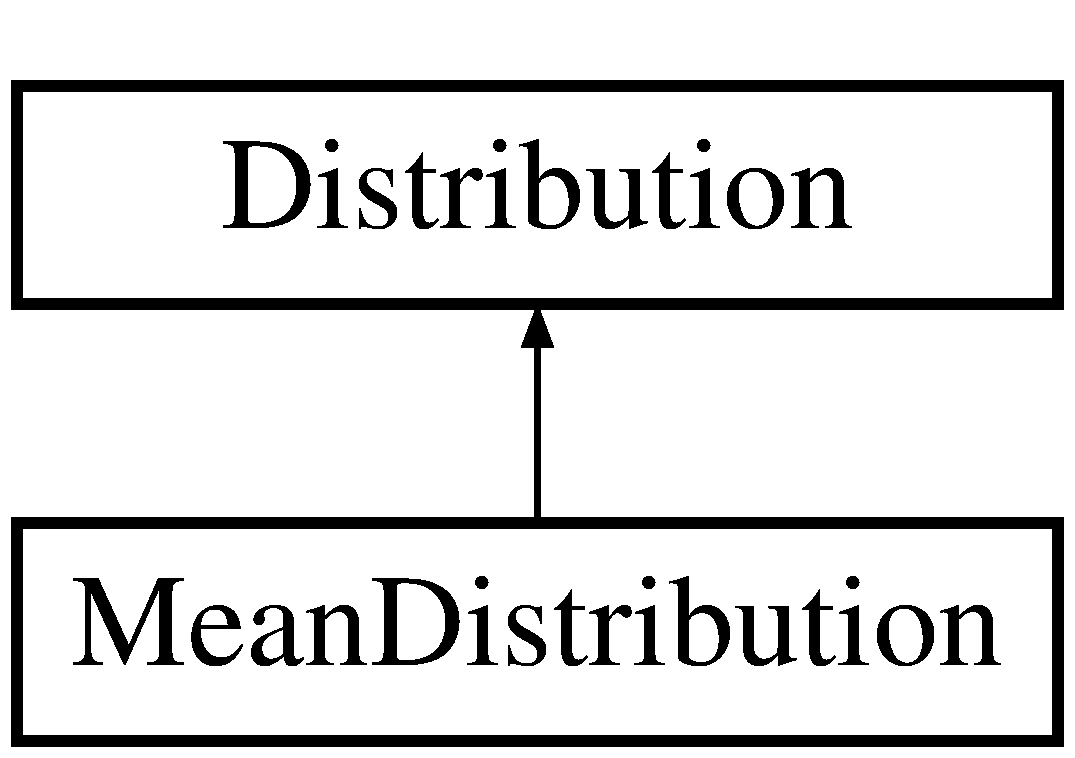
\includegraphics[height=2.000000cm]{classDistribution}
\end{center}
\end{figure}
\subsection*{Public Member Functions}
\begin{DoxyCompactItemize}
\item 
\hypertarget{classDistribution_aa7269a89c1c603c957891f49af7542e4}{}{\bfseries Distribution} (\hyperlink{classHistArray}{Hist\+Array} $\ast$hist, O\+B\+S\+Fnc fnc)\label{classDistribution_aa7269a89c1c603c957891f49af7542e4}

\item 
\hypertarget{classDistribution_a49dc0f91394f9adf82f8485ba9e12a6c}{}\hyperlink{classHistArray}{Hist\+Array} $\ast$ \hyperlink{classDistribution_a49dc0f91394f9adf82f8485ba9e12a6c}{Get\+Histograms} ()\label{classDistribution_a49dc0f91394f9adf82f8485ba9e12a6c}

\begin{DoxyCompactList}\small\item\em Return pointer to the \hyperlink{classHistArray}{Hist\+Array}. \end{DoxyCompactList}\item 
double \hyperlink{classDistribution_ab5f71f14986ae6fee369e1d3e288f793}{operator()} (const \hyperlink{classPS__2}{P\+S\+\_\+2} $\ast$ps)
\begin{DoxyCompactList}\small\item\em Evaluate the observable at the given phase space point. \end{DoxyCompactList}\item 
\hypertarget{classDistribution_a2ccf70347a37bdb98f60067ee0ac4b87}{}virtual double {\bfseries Avg} (const \hyperlink{classPS__2}{P\+S\+\_\+2} $\ast$ps)\label{classDistribution_a2ccf70347a37bdb98f60067ee0ac4b87}

\end{DoxyCompactItemize}


\subsection{Detailed Description}
The distribution class holds a pointer to a storage object (\hyperlink{classHistArray}{Hist\+Array}) and an associated observable function (O\+B\+S\+Fnc). Some predefined O\+B\+S\+Fnc\textquotesingle{}s can be found in \hyperlink{PhaseSpace_8h}{Phase\+Space.\+h}. \begin{DoxySeeAlso}{See also}
\hyperlink{PhaseSpace_8h}{Phase\+Space.\+h} 
\end{DoxySeeAlso}


Definition at line 251 of file Hist\+Array.\+h.



\subsection{Member Function Documentation}
\hypertarget{classDistribution_ab5f71f14986ae6fee369e1d3e288f793}{}\index{Distribution@{Distribution}!operator()@{operator()}}
\index{operator()@{operator()}!Distribution@{Distribution}}
\subsubsection[{operator()}]{\setlength{\rightskip}{0pt plus 5cm}double Distribution\+::operator() (
\begin{DoxyParamCaption}
\item[{const {\bf P\+S\+\_\+2} $\ast$}]{ps}
\end{DoxyParamCaption}
)\hspace{0.3cm}{\ttfamily [inline]}}\label{classDistribution_ab5f71f14986ae6fee369e1d3e288f793}


Evaluate the observable at the given phase space point. 


\begin{DoxyParams}{Parameters}
{\em ps} & Phase space point \\
\hline
\end{DoxyParams}


Definition at line 274 of file Hist\+Array.\+h.



The documentation for this class was generated from the following file\+:\begin{DoxyCompactItemize}
\item 
inc/\hyperlink{HistArray_8h}{Hist\+Array.\+h}\end{DoxyCompactItemize}

\hypertarget{structeps__entry}{\section{eps\-\_\-entry Struct Reference}
\label{structeps__entry}\index{eps\-\_\-entry@{eps\-\_\-entry}}
}
\subsection*{Public Attributes}
\begin{DoxyCompactItemize}
\item 
\hypertarget{structeps__entry_aeb23818a8c93790dc84e159e22fece7c}{int {\bfseries indices} \mbox{[}4\mbox{]}}\label{structeps__entry_aeb23818a8c93790dc84e159e22fece7c}

\item 
\hypertarget{structeps__entry_a6557cf0ea08b5afe0e6f525e13934712}{int {\bfseries sign}}\label{structeps__entry_a6557cf0ea08b5afe0e6f525e13934712}

\end{DoxyCompactItemize}


\subsection{Detailed Description}


Definition at line 599 of file Functions\-\_\-\-Shared.\-cpp.



The documentation for this struct was generated from the following file\-:\begin{DoxyCompactItemize}
\item 
src/Functions\-\_\-\-Shared.\-cpp\end{DoxyCompactItemize}

\hypertarget{classFileBrowser}{}\section{File\+Browser Class Reference}
\label{classFileBrowser}\index{File\+Browser@{File\+Browser}}


Simple, text-\/based file browser class.  




{\ttfamily \#include $<$File\+Browser.\+h$>$}

\subsection*{Public Member Functions}
\begin{DoxyCompactItemize}
\item 
\hypertarget{classFileBrowser_a6fbf64b13ec2e53f375e3e9ea3b1362a}{}\hyperlink{classFileBrowser_a6fbf64b13ec2e53f375e3e9ea3b1362a}{File\+Browser} (const std\+::string \&base\+\_\+path=\char`\"{}.\char`\"{})\label{classFileBrowser_a6fbf64b13ec2e53f375e3e9ea3b1362a}

\begin{DoxyCompactList}\small\item\em Specify base path when constructing the \hyperlink{classFileBrowser}{File\+Browser} object. \end{DoxyCompactList}\item 
\hypertarget{classFileBrowser_a188c69f0ffb1bc2510df206035fcbfd9}{}std\+::string \hyperlink{classFileBrowser_a188c69f0ffb1bc2510df206035fcbfd9}{browse} ()\label{classFileBrowser_a188c69f0ffb1bc2510df206035fcbfd9}

\begin{DoxyCompactList}\small\item\em Browse through files and folders starting at the selected base path. Returns a string with the path and name of the selected file. \end{DoxyCompactList}\item 
\hypertarget{classFileBrowser_ae65bbe179dd98f44439fc25a2e46a024}{}int {\bfseries set\+\_\+cdir} (const boost\+::filesystem\+::path \&path)\label{classFileBrowser_ae65bbe179dd98f44439fc25a2e46a024}

\end{DoxyCompactItemize}


\subsection{Detailed Description}
Simple, text-\/based file browser class. 

This is used to select files with input data for the \hyperlink{classHistArray}{Hist\+Array} objects. 

Definition at line 19 of file File\+Browser.\+h.



The documentation for this class was generated from the following files\+:\begin{DoxyCompactItemize}
\item 
inc/\hyperlink{FileBrowser_8h}{File\+Browser.\+h}\item 
src/File\+Browser.\+cpp\end{DoxyCompactItemize}

\hypertarget{classFV}{\section{F\-V Class Reference}
\label{classFV}\index{F\-V@{F\-V}}
}
\subsection*{Public Member Functions}
\begin{DoxyCompactItemize}
\item 
\hypertarget{classFV_a9b4fbb099348e0f5658290d99fcfde0f}{{\bfseries F\-V} (double const \&a=0.\-0)}\label{classFV_a9b4fbb099348e0f5658290d99fcfde0f}

\item 
\hypertarget{classFV_a7806dbe1498cda6e7b5e9deb0772915d}{{\bfseries F\-V} (\hyperlink{classFV}{F\-V} const \&rhs)}\label{classFV_a7806dbe1498cda6e7b5e9deb0772915d}

\item 
\hypertarget{classFV_a64d4ea0c4b74dd2fd557c72c30987aa5}{{\bfseries F\-V} (\hyperlink{classFV}{F\-V} \&\&rhs) noexcept}\label{classFV_a64d4ea0c4b74dd2fd557c72c30987aa5}

\item 
\hypertarget{classFV_aae9c72a65282efeadacc1b2be82b8b29}{{\bfseries F\-V} (std\-::initializer\-\_\-list$<$ double $>$ rhs)}\label{classFV_aae9c72a65282efeadacc1b2be82b8b29}

\item 
\hypertarget{classFV_addb4bbcc8d3ba7d8e94c1b6fdd006acd}{double \& {\bfseries operator\mbox{[}$\,$\mbox{]}} (int const \&i)}\label{classFV_addb4bbcc8d3ba7d8e94c1b6fdd006acd}

\item 
\hypertarget{classFV_a8c340629f03c5f4d96aefd119dd43d6e}{double const \& {\bfseries operator\mbox{[}$\,$\mbox{]}} (int const \&i) const }\label{classFV_a8c340629f03c5f4d96aefd119dd43d6e}

\item 
\hypertarget{classFV_a3ce0839ccafbead03b532cdf4af5d4c1}{\hyperlink{classFV}{F\-V} \& {\bfseries operator=} (std\-::initializer\-\_\-list$<$ double $>$ L)}\label{classFV_a3ce0839ccafbead03b532cdf4af5d4c1}

\item 
\hypertarget{classFV_aa7bad77e8a25ff4d3d769a544eccf314}{\hyperlink{classFV}{F\-V} \& {\bfseries operator=} (\hyperlink{classFV}{F\-V} const \&other)}\label{classFV_aa7bad77e8a25ff4d3d769a544eccf314}

\item 
\hypertarget{classFV_ac95050de7df77088ad31b1c755e2fe33}{\hyperlink{classFV}{F\-V} \& {\bfseries operator=} (\hyperlink{classFV}{F\-V} \&\&other) noexcept}\label{classFV_ac95050de7df77088ad31b1c755e2fe33}

\item 
\hypertarget{classFV_ac30a0c8c757d2e5dbd74131f569f48db}{\hyperlink{classFV}{F\-V} \& {\bfseries operator+=} (\hyperlink{classFV}{F\-V} const \&other)}\label{classFV_ac30a0c8c757d2e5dbd74131f569f48db}

\item 
\hypertarget{classFV_a32a55d4f37e616b0b043282a201aa0f6}{\hyperlink{classFV}{F\-V} \& {\bfseries operator-\/=} (\hyperlink{classFV}{F\-V} const \&other)}\label{classFV_a32a55d4f37e616b0b043282a201aa0f6}

\item 
\hypertarget{classFV_ac50969de8023081218ac2480f4403a4d}{\hyperlink{classFV}{F\-V} \& {\bfseries operator$\ast$=} (double const \&a)}\label{classFV_ac50969de8023081218ac2480f4403a4d}

\item 
\hypertarget{classFV_a8d74f60b130edb26fd62c590ea5ecfce}{\hyperlink{classFV}{F\-V} \& {\bfseries operator/=} (double const \&a)}\label{classFV_a8d74f60b130edb26fd62c590ea5ecfce}

\end{DoxyCompactItemize}
\subsection*{Protected Attributes}
\begin{DoxyCompactItemize}
\item 
\hypertarget{classFV_a909196132ec1cd190f8c01546ea5bced}{double {\bfseries v} \mbox{[}4\mbox{]}}\label{classFV_a909196132ec1cd190f8c01546ea5bced}

\end{DoxyCompactItemize}


The documentation for this class was generated from the following files\-:\begin{DoxyCompactItemize}
\item 
inc/Lorentz.\-h\item 
src/Lorentz.\-cpp\end{DoxyCompactItemize}

\hypertarget{structpVEGAS_1_1gsl__monte__vegas__state}{\section{p\-V\-E\-G\-A\-S\-:\-:gsl\-\_\-monte\-\_\-vegas\-\_\-state Struct Reference}
\label{structpVEGAS_1_1gsl__monte__vegas__state}\index{p\-V\-E\-G\-A\-S\-::gsl\-\_\-monte\-\_\-vegas\-\_\-state@{p\-V\-E\-G\-A\-S\-::gsl\-\_\-monte\-\_\-vegas\-\_\-state}}
}
\subsection*{Public Attributes}
\begin{DoxyCompactItemize}
\item 
\hypertarget{structpVEGAS_1_1gsl__monte__vegas__state_ad90199fbfe96d952b3ddd5d9ee50d7d6}{double {\bfseries alpha}}\label{structpVEGAS_1_1gsl__monte__vegas__state_ad90199fbfe96d952b3ddd5d9ee50d7d6}

\item 
\hypertarget{structpVEGAS_1_1gsl__monte__vegas__state_a39b883f4a437280c3e5d5b5e07f111a3}{int {\bfseries mode}}\label{structpVEGAS_1_1gsl__monte__vegas__state_a39b883f4a437280c3e5d5b5e07f111a3}

\item 
\hypertarget{structpVEGAS_1_1gsl__monte__vegas__state_acdde9366a7d66391f14c27ad0b96cafa}{int {\bfseries verbose}}\label{structpVEGAS_1_1gsl__monte__vegas__state_acdde9366a7d66391f14c27ad0b96cafa}

\item 
\hypertarget{structpVEGAS_1_1gsl__monte__vegas__state_a5f12f3e4474770bbb6e1d0256e872b09}{unsigned int {\bfseries iterations}}\label{structpVEGAS_1_1gsl__monte__vegas__state_a5f12f3e4474770bbb6e1d0256e872b09}

\item 
\hypertarget{structpVEGAS_1_1gsl__monte__vegas__state_aee953f39aec5f8650863d3cc43efe111}{int {\bfseries stage}}\label{structpVEGAS_1_1gsl__monte__vegas__state_aee953f39aec5f8650863d3cc43efe111}

\item 
\hypertarget{structpVEGAS_1_1gsl__monte__vegas__state_a26732c04d9dbe43bc7421866cb5990c7}{size\-\_\-t {\bfseries dim}}\label{structpVEGAS_1_1gsl__monte__vegas__state_a26732c04d9dbe43bc7421866cb5990c7}

\item 
\hypertarget{structpVEGAS_1_1gsl__monte__vegas__state_a92f422cf2d6586001d785c674cc00bb7}{size\-\_\-t {\bfseries bins\-\_\-max}}\label{structpVEGAS_1_1gsl__monte__vegas__state_a92f422cf2d6586001d785c674cc00bb7}

\item 
\hypertarget{structpVEGAS_1_1gsl__monte__vegas__state_ae89112de0dd422096c5695939e9a2b04}{double {\bfseries vol}}\label{structpVEGAS_1_1gsl__monte__vegas__state_ae89112de0dd422096c5695939e9a2b04}

\item 
\hypertarget{structpVEGAS_1_1gsl__monte__vegas__state_aa907e8fcf149f5c3d10fd39bf6847f1b}{double $\ast$ {\bfseries delx}}\label{structpVEGAS_1_1gsl__monte__vegas__state_aa907e8fcf149f5c3d10fd39bf6847f1b}

\item 
\hypertarget{structpVEGAS_1_1gsl__monte__vegas__state_ae49b6fe8a2bece086de1c57f80d14f9d}{unsigned int {\bfseries bins}}\label{structpVEGAS_1_1gsl__monte__vegas__state_ae49b6fe8a2bece086de1c57f80d14f9d}

\item 
\hypertarget{structpVEGAS_1_1gsl__monte__vegas__state_ab7a477d830b6673def7fbdc0a40cda41}{unsigned int {\bfseries boxes}}\label{structpVEGAS_1_1gsl__monte__vegas__state_ab7a477d830b6673def7fbdc0a40cda41}

\item 
\hypertarget{structpVEGAS_1_1gsl__monte__vegas__state_a684e486d9faed388313c8dd84145b307}{double $\ast$ {\bfseries xi}}\label{structpVEGAS_1_1gsl__monte__vegas__state_a684e486d9faed388313c8dd84145b307}

\item 
\hypertarget{structpVEGAS_1_1gsl__monte__vegas__state_aecbb3921cf6bc3424df1a7cd85180cde}{double $\ast$ {\bfseries d}}\label{structpVEGAS_1_1gsl__monte__vegas__state_aecbb3921cf6bc3424df1a7cd85180cde}

\item 
\hypertarget{structpVEGAS_1_1gsl__monte__vegas__state_a192893e283dd35f5ac83d0299dee9264}{double $\ast$ {\bfseries xin}}\label{structpVEGAS_1_1gsl__monte__vegas__state_a192893e283dd35f5ac83d0299dee9264}

\item 
\hypertarget{structpVEGAS_1_1gsl__monte__vegas__state_a89740accd284b8e9f3f6293dd34cc3d5}{double $\ast$ {\bfseries weight}}\label{structpVEGAS_1_1gsl__monte__vegas__state_a89740accd284b8e9f3f6293dd34cc3d5}

\item 
\hypertarget{structpVEGAS_1_1gsl__monte__vegas__state_ae1f2f226bf1925224fdc53a83af17254}{double $\ast$$\ast$ {\bfseries x}}\label{structpVEGAS_1_1gsl__monte__vegas__state_ae1f2f226bf1925224fdc53a83af17254}

\item 
\hypertarget{structpVEGAS_1_1gsl__monte__vegas__state_a70b17fa6eefe644a675154db73753834}{int $\ast$$\ast$ {\bfseries bin}}\label{structpVEGAS_1_1gsl__monte__vegas__state_a70b17fa6eefe644a675154db73753834}

\item 
\hypertarget{structpVEGAS_1_1gsl__monte__vegas__state_a424168553bea12fe19d487199273a671}{int $\ast$$\ast$ {\bfseries box}}\label{structpVEGAS_1_1gsl__monte__vegas__state_a424168553bea12fe19d487199273a671}

\item 
\hypertarget{structpVEGAS_1_1gsl__monte__vegas__state_a98ccf83d7fe8fed7508035c4dd65250e}{double $\ast$ {\bfseries bin\-\_\-vol}}\label{structpVEGAS_1_1gsl__monte__vegas__state_a98ccf83d7fe8fed7508035c4dd65250e}

\item 
\hypertarget{structpVEGAS_1_1gsl__monte__vegas__state_a421ec0cc180f1f5e62446cc11ac63ac1}{double {\bfseries wgt}}\label{structpVEGAS_1_1gsl__monte__vegas__state_a421ec0cc180f1f5e62446cc11ac63ac1}

\item 
\hypertarget{structpVEGAS_1_1gsl__monte__vegas__state_aced257612814bf353e2737870affe633}{double {\bfseries jac}}\label{structpVEGAS_1_1gsl__monte__vegas__state_aced257612814bf353e2737870affe633}

\item 
\hypertarget{structpVEGAS_1_1gsl__monte__vegas__state_ad6411f8f95160c1a1f6242ed0e71f304}{double {\bfseries wtd\-\_\-int\-\_\-sum}}\label{structpVEGAS_1_1gsl__monte__vegas__state_ad6411f8f95160c1a1f6242ed0e71f304}

\item 
\hypertarget{structpVEGAS_1_1gsl__monte__vegas__state_a27c8b415c4fbc515f398a2995c67fef4}{double {\bfseries sum\-\_\-wgts}}\label{structpVEGAS_1_1gsl__monte__vegas__state_a27c8b415c4fbc515f398a2995c67fef4}

\item 
\hypertarget{structpVEGAS_1_1gsl__monte__vegas__state_a2e84a42cd260138800d884c504470849}{double {\bfseries chi\-\_\-sum}}\label{structpVEGAS_1_1gsl__monte__vegas__state_a2e84a42cd260138800d884c504470849}

\item 
\hypertarget{structpVEGAS_1_1gsl__monte__vegas__state_af4e41ee939643e0ec5bf1f8d5738aead}{double {\bfseries chisq}}\label{structpVEGAS_1_1gsl__monte__vegas__state_af4e41ee939643e0ec5bf1f8d5738aead}

\item 
\hypertarget{structpVEGAS_1_1gsl__monte__vegas__state_ab773910457bfec6c983a389d1714c4b6}{double {\bfseries result}}\label{structpVEGAS_1_1gsl__monte__vegas__state_ab773910457bfec6c983a389d1714c4b6}

\item 
\hypertarget{structpVEGAS_1_1gsl__monte__vegas__state_aca33e0298b14ffcb4fbf45df4ca4d41a}{double {\bfseries sigma}}\label{structpVEGAS_1_1gsl__monte__vegas__state_aca33e0298b14ffcb4fbf45df4ca4d41a}

\item 
\hypertarget{structpVEGAS_1_1gsl__monte__vegas__state_ae4e55b3cc72ef59e0a40c47f52976c66}{unsigned int {\bfseries it\-\_\-start}}\label{structpVEGAS_1_1gsl__monte__vegas__state_ae4e55b3cc72ef59e0a40c47f52976c66}

\item 
\hypertarget{structpVEGAS_1_1gsl__monte__vegas__state_aa1a2ebd4a0a5d122a313772428f2a0ea}{unsigned int {\bfseries it\-\_\-num}}\label{structpVEGAS_1_1gsl__monte__vegas__state_aa1a2ebd4a0a5d122a313772428f2a0ea}

\item 
\hypertarget{structpVEGAS_1_1gsl__monte__vegas__state_a60d520a64ceb65614d546bb53a2a6312}{unsigned int {\bfseries samples}}\label{structpVEGAS_1_1gsl__monte__vegas__state_a60d520a64ceb65614d546bb53a2a6312}

\item 
\hypertarget{structpVEGAS_1_1gsl__monte__vegas__state_ac66ba96628f4a1f54086f63723205d0a}{unsigned int {\bfseries calls\-\_\-per\-\_\-box}}\label{structpVEGAS_1_1gsl__monte__vegas__state_ac66ba96628f4a1f54086f63723205d0a}

\item 
\hypertarget{structpVEGAS_1_1gsl__monte__vegas__state_a25f3309b26c45774a9a7f5ab2b79dad1}{size\-\_\-t {\bfseries num\-\_\-threads}}\label{structpVEGAS_1_1gsl__monte__vegas__state_a25f3309b26c45774a9a7f5ab2b79dad1}

\item 
\hypertarget{structpVEGAS_1_1gsl__monte__vegas__state_a7a2be2f94c124e06e0acbdcc824770f9}{F\-I\-L\-E $\ast$ {\bfseries ostream}}\label{structpVEGAS_1_1gsl__monte__vegas__state_a7a2be2f94c124e06e0acbdcc824770f9}

\end{DoxyCompactItemize}


\subsection{Detailed Description}


Definition at line 69 of file p\-V\-E\-G\-A\-S.\-h.



The documentation for this struct was generated from the following file\-:\begin{DoxyCompactItemize}
\item 
inc/\hyperlink{pVEGAS_8h}{p\-V\-E\-G\-A\-S.\-h}\end{DoxyCompactItemize}

\hypertarget{classHiggsBoson}{}\section{Higgs\+Boson Class Reference}
\label{classHiggsBoson}\index{Higgs\+Boson@{Higgs\+Boson}}


{\ttfamily \#include $<$Higgs\+Model.\+h$>$}

\subsection*{Public Member Functions}
\begin{DoxyCompactItemize}
\item 
\hypertarget{classHiggsBoson_aef7e66e7df2850281117c8065f86266a}{}{\bfseries Higgs\+Boson} (double const \&M, double const \&G, double const \&Vh, double const \&At, double const \&Bt, double const \&Ab=0.\+0, double const \&Bb=0.\+0)\label{classHiggsBoson_aef7e66e7df2850281117c8065f86266a}

\item 
\hypertarget{classHiggsBoson_a3a18ef5458760d0b4fe6f7f67847f200}{}double const \& {\bfseries M} () const \label{classHiggsBoson_a3a18ef5458760d0b4fe6f7f67847f200}

\item 
\hypertarget{classHiggsBoson_a1cbc3cabab562910857fd24602c88029}{}double const \& {\bfseries M2} () const \label{classHiggsBoson_a1cbc3cabab562910857fd24602c88029}

\item 
\hypertarget{classHiggsBoson_abee4eef942de0a4088166fa59b09054e}{}double const \& {\bfseries G} () const \label{classHiggsBoson_abee4eef942de0a4088166fa59b09054e}

\item 
\hypertarget{classHiggsBoson_aee7be204e7532152c97f6115632c76ac}{}double const \& {\bfseries G2} () const \label{classHiggsBoson_aee7be204e7532152c97f6115632c76ac}

\item 
\hypertarget{classHiggsBoson_a56fe580ffe65572242ba5170c5f95126}{}double const \& {\bfseries At} () const \label{classHiggsBoson_a56fe580ffe65572242ba5170c5f95126}

\item 
\hypertarget{classHiggsBoson_a0919c5fc894bb010490229271e781bdd}{}double const \& {\bfseries Bt} () const \label{classHiggsBoson_a0919c5fc894bb010490229271e781bdd}

\item 
\hypertarget{classHiggsBoson_a15a4d40ec981360f0c1033d5c7156c99}{}double const \& {\bfseries Ab} () const \label{classHiggsBoson_a15a4d40ec981360f0c1033d5c7156c99}

\item 
\hypertarget{classHiggsBoson_ad4dc9de0ef7ca8a9c2edb8884e41bd88}{}double const \& {\bfseries Bb} () const \label{classHiggsBoson_ad4dc9de0ef7ca8a9c2edb8884e41bd88}

\item 
\hypertarget{classHiggsBoson_a9b4cda666fb19288713b334bb72e3b40}{}void {\bfseries Set\+M} (double const \&val)\label{classHiggsBoson_a9b4cda666fb19288713b334bb72e3b40}

\item 
\hypertarget{classHiggsBoson_a89f471e351c72fcf5e95846b34727383}{}\hyperlink{Global_8h_af390c6bd8192faf6a1e2d875a1d10ca0}{c\+\_\+double} const \& {\bfseries Get\+F\+H0} () const \label{classHiggsBoson_a89f471e351c72fcf5e95846b34727383}

\item 
\hypertarget{classHiggsBoson_a2be84efb1f350882309f74db3dcc32a5}{}\hyperlink{Global_8h_af390c6bd8192faf6a1e2d875a1d10ca0}{c\+\_\+double} const \& {\bfseries Get\+F\+A0} () const \label{classHiggsBoson_a2be84efb1f350882309f74db3dcc32a5}

\item 
void \hyperlink{classHiggsBoson_a4edd830907f5f06ac24deed99e64da0c}{Set\+Form\+Factors} (double const \&S, double const \&mt2, double const \&mb2)
\begin{DoxyCompactList}\small\item\em Compute 1-\/loop form factors for given c.\+m.\+e., top-\/ and bottom mass and store values in member variables. Note that the form factors are recomputed only if the c.\+m.\+e. changes (compared to last call)! The values stored in the respective member variables are -\/ F\+\_\+s / (4 s) and F\+\_\+p / (8 s). \end{DoxyCompactList}\item 
\hypertarget{classHiggsBoson_a6e3be51e54f71ad1681485d463ba54f9}{}\hyperlink{Global_8h_af390c6bd8192faf6a1e2d875a1d10ca0}{c\+\_\+double} const \& {\bfseries Get\+Fs} () const \label{classHiggsBoson_a6e3be51e54f71ad1681485d463ba54f9}

\item 
\hypertarget{classHiggsBoson_a404990102de3ee3cd1f65a53f0759d76}{}\hyperlink{Global_8h_af390c6bd8192faf6a1e2d875a1d10ca0}{c\+\_\+double} const \& {\bfseries Get\+Fp} () const \label{classHiggsBoson_a404990102de3ee3cd1f65a53f0759d76}

\item 
\hypertarget{classHiggsBoson_af9055e140206943efe94b55ea76c1632}{}\hyperlink{Global_8h_af390c6bd8192faf6a1e2d875a1d10ca0}{c\+\_\+double} const \& \hyperlink{classHiggsBoson_af9055e140206943efe94b55ea76c1632}{Get\+F\+H} (bool E\+F\+F) const \label{classHiggsBoson_af9055e140206943efe94b55ea76c1632}

\begin{DoxyCompactList}\small\item\em returns effective gg-\/scalar coupling if E\+F\+F=true, full 1-\/loop form factor otherwise \end{DoxyCompactList}\item 
\hypertarget{classHiggsBoson_a8af3de930fb155b566956ab7c0457e29}{}\hyperlink{Global_8h_af390c6bd8192faf6a1e2d875a1d10ca0}{c\+\_\+double} const \& \hyperlink{classHiggsBoson_a8af3de930fb155b566956ab7c0457e29}{Get\+F\+A} (bool E\+F\+F) const \label{classHiggsBoson_a8af3de930fb155b566956ab7c0457e29}

\begin{DoxyCompactList}\small\item\em returns effective gg-\/pseudoscalar coupling if E\+F\+F=true, full 1-\/loop form factor otherwise \end{DoxyCompactList}\item 
void \hyperlink{classHiggsBoson_afebe4ad11ea2cbc2ec0ed1b94759c293}{Set\+Propagator} (double const \&S, bool rescale=false)
\begin{DoxyCompactList}\small\item\em compute propagator value for given c.\+m.\+e. and store values in member variables \end{DoxyCompactList}\item 
\hypertarget{classHiggsBoson_a3b836f00cee69f41cd04dd61e86bc4ab}{}double const \& {\bfseries Get\+Propagator\+Sq} () const \label{classHiggsBoson_a3b836f00cee69f41cd04dd61e86bc4ab}

\item 
\hypertarget{classHiggsBoson_abc21bb217a9a176025516e429a6c25ee}{}\hyperlink{Global_8h_af390c6bd8192faf6a1e2d875a1d10ca0}{c\+\_\+double} const \& {\bfseries Get\+Propagator} () const \label{classHiggsBoson_abc21bb217a9a176025516e429a6c25ee}

\end{DoxyCompactItemize}


\subsection{Detailed Description}
This class contains the parameters that describe a single neutral Higgs boson. \begin{DoxySeeAlso}{See also}
\hyperlink{classHiggsModel}{Higgs\+Model} 
\end{DoxySeeAlso}


Definition at line 48 of file Higgs\+Model.\+h.



\subsection{Member Function Documentation}
\hypertarget{classHiggsBoson_a4edd830907f5f06ac24deed99e64da0c}{}\index{Higgs\+Boson@{Higgs\+Boson}!Set\+Form\+Factors@{Set\+Form\+Factors}}
\index{Set\+Form\+Factors@{Set\+Form\+Factors}!Higgs\+Boson@{Higgs\+Boson}}
\subsubsection[{Set\+Form\+Factors}]{\setlength{\rightskip}{0pt plus 5cm}void Higgs\+Boson\+::\+Set\+Form\+Factors (
\begin{DoxyParamCaption}
\item[{double const \&}]{S, }
\item[{double const \&}]{mt2, }
\item[{double const \&}]{mb2}
\end{DoxyParamCaption}
)}\label{classHiggsBoson_a4edd830907f5f06ac24deed99e64da0c}


Compute 1-\/loop form factors for given c.\+m.\+e., top-\/ and bottom mass and store values in member variables. Note that the form factors are recomputed only if the c.\+m.\+e. changes (compared to last call)! The values stored in the respective member variables are -\/ F\+\_\+s / (4 s) and F\+\_\+p / (8 s). 


\begin{DoxyParams}{Parameters}
{\em S} & c.\+m.\+e. \\
\hline
{\em mt2} & top-\/mass squared \\
\hline
{\em mb2} & bottom-\/mass squared \\
\hline
\end{DoxyParams}


Definition at line 47 of file Higgs\+Model.\+cpp.

\hypertarget{classHiggsBoson_afebe4ad11ea2cbc2ec0ed1b94759c293}{}\index{Higgs\+Boson@{Higgs\+Boson}!Set\+Propagator@{Set\+Propagator}}
\index{Set\+Propagator@{Set\+Propagator}!Higgs\+Boson@{Higgs\+Boson}}
\subsubsection[{Set\+Propagator}]{\setlength{\rightskip}{0pt plus 5cm}void Higgs\+Boson\+::\+Set\+Propagator (
\begin{DoxyParamCaption}
\item[{double const \&}]{S, }
\item[{bool}]{rescale = {\ttfamily false}}
\end{DoxyParamCaption}
)}\label{classHiggsBoson_afebe4ad11ea2cbc2ec0ed1b94759c293}


compute propagator value for given c.\+m.\+e. and store values in member variables 


\begin{DoxyParams}{Parameters}
{\em S} & momentum squared in the Higgs propagators \\
\hline
\end{DoxyParams}


Definition at line 107 of file Higgs\+Model.\+cpp.



The documentation for this class was generated from the following files\+:\begin{DoxyCompactItemize}
\item 
inc/\hyperlink{HiggsModel_8h}{Higgs\+Model.\+h}\item 
src/Higgs\+Model.\+cpp\end{DoxyCompactItemize}

\hypertarget{classHiggsModel}{}\section{Higgs\+Model Class Reference}
\label{classHiggsModel}\index{Higgs\+Model@{Higgs\+Model}}


This class contains all the physical, model specific parameters.  




{\ttfamily \#include $<$Higgs\+Model.\+h$>$}

\subsection*{Public Member Functions}
\begin{DoxyCompactItemize}
\item 
\hypertarget{classHiggsModel_aa6f39f73df22008fa639fd64653cc8e2}{}{\bfseries Higgs\+Model} (std\+::string const \&name=\char`\"{}noname\char`\"{})\label{classHiggsModel_aa6f39f73df22008fa639fd64653cc8e2}

\item 
\hypertarget{classHiggsModel_a29a94aee623c9ce8d874b8b4fba17835}{}std\+::string const \& {\bfseries Name} () const \label{classHiggsModel_a29a94aee623c9ce8d874b8b4fba17835}

\item 
\hypertarget{classHiggsModel_a343a0ea0a7a22e78c3504dc64d4d6184}{}double const \& {\bfseries Alpha\+S} () const \label{classHiggsModel_a343a0ea0a7a22e78c3504dc64d4d6184}

\item 
\hypertarget{classHiggsModel_a41c108f3545d39dbb23835d781a163ee}{}double const \& {\bfseries Alpha\+S2} () const \label{classHiggsModel_a41c108f3545d39dbb23835d781a163ee}

\item 
\hypertarget{classHiggsModel_aca6071e5666fa030cacb0a11efaa1f22}{}double const \& {\bfseries M\+U\+R} () const \label{classHiggsModel_aca6071e5666fa030cacb0a11efaa1f22}

\item 
\hypertarget{classHiggsModel_a2f76729834fcbab6bb0b8c8595c05983}{}double const \& {\bfseries M\+U\+R2} () const \label{classHiggsModel_a2f76729834fcbab6bb0b8c8595c05983}

\item 
\hypertarget{classHiggsModel_a24085f73b5e2858e86db20470f8e5c9f}{}double const \& {\bfseries M\+U\+F} () const \label{classHiggsModel_a24085f73b5e2858e86db20470f8e5c9f}

\item 
\hypertarget{classHiggsModel_af636a81480654395084ead903d5ee00b}{}double const \& {\bfseries M\+U\+F2} () const \label{classHiggsModel_af636a81480654395084ead903d5ee00b}

\item 
\hypertarget{classHiggsModel_a913923ce15ea38a8a1576ea9e5d23d10}{}double const \& {\bfseries mt} () const \label{classHiggsModel_a913923ce15ea38a8a1576ea9e5d23d10}

\item 
\hypertarget{classHiggsModel_ad0685a0848a95342b272147317948d10}{}double const \& {\bfseries mt2} () const \label{classHiggsModel_ad0685a0848a95342b272147317948d10}

\item 
\hypertarget{classHiggsModel_a8ec3f6255ab720fb08a94937d436cdea}{}double const \& {\bfseries mb} () const \label{classHiggsModel_a8ec3f6255ab720fb08a94937d436cdea}

\item 
\hypertarget{classHiggsModel_a33ea2c639935f9971bdca5e5994325ff}{}double const \& {\bfseries mb2} () const \label{classHiggsModel_a33ea2c639935f9971bdca5e5994325ff}

\item 
\hypertarget{classHiggsModel_a9711ab1e2b584f86d75f6e53b9a35822}{}double const \& {\bfseries V\+H} () const \label{classHiggsModel_a9711ab1e2b584f86d75f6e53b9a35822}

\item 
\hypertarget{classHiggsModel_af679483d403b1d8b2f291542215fa0bd}{}double const \& {\bfseries Scale} () const \label{classHiggsModel_af679483d403b1d8b2f291542215fa0bd}

\item 
\hypertarget{classHiggsModel_a2572b90895176763db5cbbb3233ec242}{}double const \& {\bfseries Scale2} () const \label{classHiggsModel_a2572b90895176763db5cbbb3233ec242}

\item 
\hypertarget{classHiggsModel_a08c33da1ef0b46ed04dd5f1f9f84ae9a}{}int {\bfseries N\+Bosons} () const \label{classHiggsModel_a08c33da1ef0b46ed04dd5f1f9f84ae9a}

\item 
\hypertarget{classHiggsModel_a56909ae8843fbd15bc54df272e1a245d}{}std\+::vector$<$ H\+Ptr $>$ const \& {\bfseries Get\+Bosons} () const \label{classHiggsModel_a56909ae8843fbd15bc54df272e1a245d}

\item 
\hypertarget{classHiggsModel_a4b3180e3b5172e9a3fcde3f2740d2eb0}{}void {\bfseries Clear\+Bosons} ()\label{classHiggsModel_a4b3180e3b5172e9a3fcde3f2740d2eb0}

\item 
\hypertarget{classHiggsModel_afa9a44f6a2bd358d887acd5771253953}{}H\+Ptr {\bfseries Get\+Boson} (int i)\label{classHiggsModel_afa9a44f6a2bd358d887acd5771253953}

\item 
\hypertarget{classHiggsModel_ae082694ec944cffd807f4f0a20bf931b}{}H\+Ptr const {\bfseries Get\+Boson} (int i) const \label{classHiggsModel_ae082694ec944cffd807f4f0a20bf931b}

\item 
\hypertarget{classHiggsModel_a5a3f7171856b2106141948544fc49f13}{}void \hyperlink{classHiggsModel_a5a3f7171856b2106141948544fc49f13}{Set\+Alpha\+S} (double const \&val)\label{classHiggsModel_a5a3f7171856b2106141948544fc49f13}

\begin{DoxyCompactList}\small\item\em Use this member to change Alpha\+S. It automatically resets the values of the amplitude prefactors. \end{DoxyCompactList}\item 
\hypertarget{classHiggsModel_a40b498b2555458a9abc4ea989e72ce91}{}void {\bfseries Set\+M\+U\+R} (double const \&val)\label{classHiggsModel_a40b498b2555458a9abc4ea989e72ce91}

\item 
\hypertarget{classHiggsModel_a8e8772814f7441352b226eb0566a263e}{}void {\bfseries Set\+M\+U\+F} (double const \&val)\label{classHiggsModel_a8e8772814f7441352b226eb0566a263e}

\item 
\hypertarget{classHiggsModel_a511bd13bf20268e59567b2049d7a5781}{}void {\bfseries Set\+Mt} (double const \&val)\label{classHiggsModel_a511bd13bf20268e59567b2049d7a5781}

\item 
\hypertarget{classHiggsModel_a460c285dbbd117c30be6ea43f5271e2d}{}void {\bfseries Set\+Mb} (double const \&val)\label{classHiggsModel_a460c285dbbd117c30be6ea43f5271e2d}

\item 
\hypertarget{classHiggsModel_a058daf0cc3b8cad4077419d19d8e4c21}{}void {\bfseries Set\+V\+H} (double const \&val)\label{classHiggsModel_a058daf0cc3b8cad4077419d19d8e4c21}

\item 
\hypertarget{classHiggsModel_aaca4ad2dcfd40c87e76fc88ab95b56dc}{}void {\bfseries Set\+Scale} (double const \&val)\label{classHiggsModel_aaca4ad2dcfd40c87e76fc88ab95b56dc}

\item 
\hypertarget{classHiggsModel_a0f932c9eddbc1d0f93b97135c2db468d}{}void {\bfseries Set\+Use\+K} (bool k)\label{classHiggsModel_a0f932c9eddbc1d0f93b97135c2db468d}

\item 
\hypertarget{classHiggsModel_acd450a454977065794aa76695963c8eb}{}bool {\bfseries Use\+K} ()\label{classHiggsModel_acd450a454977065794aa76695963c8eb}

\item 
void \hyperlink{classHiggsModel_a43f6951291eef31cc18116f7d49f839f}{Set\+Higgs\+Prefactors} (double const \&S, bool E\+F\+F)
\begin{DoxyCompactList}\small\item\em Reset values of the Higgs prefactors. All Higgs bosons in the vector d\+\_\+\+Bosons will be taken into account. \end{DoxyCompactList}\item 
\hypertarget{classHiggsModel_a36b052bac528028a1757554d45901513}{}\hyperlink{structHiggsPrefactors}{Higgs\+Prefactors} const \& {\bfseries Get\+Higgs\+Prefactors} () const \label{classHiggsModel_a36b052bac528028a1757554d45901513}

\item 
\hypertarget{classHiggsModel_a514e3dd7854409c622b8e200fe2ee84c}{}void \hyperlink{classHiggsModel_a514e3dd7854409c622b8e200fe2ee84c}{Set\+Amp\+Prefactors} ()\label{classHiggsModel_a514e3dd7854409c622b8e200fe2ee84c}

\begin{DoxyCompactList}\small\item\em Reset values of the amplitude prefactors. \end{DoxyCompactList}\item 
\hypertarget{classHiggsModel_a77b35a425c80b8d9006354670f91acca}{}\hyperlink{structAmplitudePrefactors}{Amplitude\+Prefactors} const \& {\bfseries Get\+Amp\+Prefactors} () const \label{classHiggsModel_a77b35a425c80b8d9006354670f91acca}

\item 
void \hyperlink{classHiggsModel_acd87bf9a85c37da737aba62a0dc82b5b}{Add\+Boson} (double const \&M, double const \&G, double const \&a\+\_\+t=1.\+0, double const \&b\+\_\+t=1.\+0, double const \&a\+\_\+b=0.\+0, double const \&b\+\_\+b=0.\+0)
\begin{DoxyCompactList}\small\item\em Add a Higgs boson to the vector d\+\_\+\+Bosons. The dimensionful parameters M and G will be rescaled with d\+\_\+\+Scale. \end{DoxyCompactList}\item 
void \hyperlink{classHiggsModel_ab84c9016bf5a8bd87f82f214c34cce8b}{Add\+Scalar} (double const \&M, double const \&G, double const \&a\+\_\+t=1.\+0, double const \&a\+\_\+b=0.\+0)
\begin{DoxyCompactList}\small\item\em Add a scalar Higgs boson to the vector d\+\_\+\+Bosons. The dimensionful parameters M and G will be rescaled with d\+\_\+\+Scale. \end{DoxyCompactList}\item 
void \hyperlink{classHiggsModel_a94f5b60024363838e73e0e1b8d1604ca}{Add\+Pseudoscalar} (double const \&M, double const \&G, double const \&b\+\_\+t=1.\+0, double const \&b\+\_\+b=0.\+0)
\begin{DoxyCompactList}\small\item\em Add a pseudoscalar Higgs boson to the vector d\+\_\+\+Bosons. The dimensionful parameters M and G will be rescaled with d\+\_\+\+Scale. \end{DoxyCompactList}\item 
\hypertarget{classHiggsModel_a7aea18c2e6622159e8f6cc29be537c0f}{}void \hyperlink{classHiggsModel_a7aea18c2e6622159e8f6cc29be537c0f}{Pop\+Boson} ()\label{classHiggsModel_a7aea18c2e6622159e8f6cc29be537c0f}

\begin{DoxyCompactList}\small\item\em Remove the last Higgs boson added to the vector d\+\_\+\+Bosons. \end{DoxyCompactList}\item 
void \hyperlink{classHiggsModel_a71e8fcd730feb01afd4c39f3cd184655}{Print} (std\+::ostream \&ost, double const \&m\+Scale) const 
\begin{DoxyCompactList}\small\item\em Print the model parameters. \end{DoxyCompactList}\end{DoxyCompactItemize}


\subsection{Detailed Description}
This class contains all the physical, model specific parameters. 

These are the strong coupling Alpha\+S, renormalization and factorization scales M\+U\+R, M\+U\+F, the third generation quark masses mt and mb as well as the combined Higgs vacuum expectation value V\+H and the individual Higgs boson parameters. It also provides appropriate setter functions. It contains instances of the \hyperlink{structHiggsPrefactors}{Higgs\+Prefactors} and Amprefactors structures that are needed for the evaluation of the amplitudes. Take care to provide numerical values consistently in the same units. \begin{DoxySeeAlso}{See also}
Amp\+Prefactors, \hyperlink{structHiggsPrefactors}{Higgs\+Prefactors}, \hyperlink{classHiggsBoson}{Higgs\+Boson} 
\end{DoxySeeAlso}


Definition at line 243 of file Higgs\+Model.\+h.



\subsection{Member Function Documentation}
\hypertarget{classHiggsModel_acd87bf9a85c37da737aba62a0dc82b5b}{}\index{Higgs\+Model@{Higgs\+Model}!Add\+Boson@{Add\+Boson}}
\index{Add\+Boson@{Add\+Boson}!Higgs\+Model@{Higgs\+Model}}
\subsubsection[{Add\+Boson}]{\setlength{\rightskip}{0pt plus 5cm}void Higgs\+Model\+::\+Add\+Boson (
\begin{DoxyParamCaption}
\item[{double const \&}]{M, }
\item[{double const \&}]{G, }
\item[{double const \&}]{a\+\_\+t = {\ttfamily 1.0}, }
\item[{double const \&}]{b\+\_\+t = {\ttfamily 1.0}, }
\item[{double const \&}]{a\+\_\+b = {\ttfamily 0.0}, }
\item[{double const \&}]{b\+\_\+b = {\ttfamily 0.0}}
\end{DoxyParamCaption}
)}\label{classHiggsModel_acd87bf9a85c37da737aba62a0dc82b5b}


Add a Higgs boson to the vector d\+\_\+\+Bosons. The dimensionful parameters M and G will be rescaled with d\+\_\+\+Scale. 


\begin{DoxyParams}{Parameters}
{\em M} & mass \\
\hline
{\em G} & width \\
\hline
{\em a\+\_\+t} & reduced scalar coupling to the top-\/quark \\
\hline
{\em b\+\_\+t} & reduced pseudoscalar coupling to the top-\/quark \\
\hline
{\em a\+\_\+t} & reduced scalar coupling to the bottom-\/quark \\
\hline
{\em b\+\_\+t} & reduced pseudoscalar coupling to the bottom-\/quark \\
\hline
\end{DoxyParams}


Definition at line 447 of file Higgs\+Model.\+cpp.

\hypertarget{classHiggsModel_a94f5b60024363838e73e0e1b8d1604ca}{}\index{Higgs\+Model@{Higgs\+Model}!Add\+Pseudoscalar@{Add\+Pseudoscalar}}
\index{Add\+Pseudoscalar@{Add\+Pseudoscalar}!Higgs\+Model@{Higgs\+Model}}
\subsubsection[{Add\+Pseudoscalar}]{\setlength{\rightskip}{0pt plus 5cm}void Higgs\+Model\+::\+Add\+Pseudoscalar (
\begin{DoxyParamCaption}
\item[{double const \&}]{M, }
\item[{double const \&}]{G, }
\item[{double const \&}]{b\+\_\+t = {\ttfamily 1.0}, }
\item[{double const \&}]{b\+\_\+b = {\ttfamily 0.0}}
\end{DoxyParamCaption}
)}\label{classHiggsModel_a94f5b60024363838e73e0e1b8d1604ca}


Add a pseudoscalar Higgs boson to the vector d\+\_\+\+Bosons. The dimensionful parameters M and G will be rescaled with d\+\_\+\+Scale. 


\begin{DoxyParams}{Parameters}
{\em M} & mass \\
\hline
{\em G} & width \\
\hline
{\em b\+\_\+t} & reduced pseudoscalar coupling to the top-\/quark \\
\hline
{\em b\+\_\+t} & reduced pseudoscalar coupling to the bottom-\/quark \\
\hline
\end{DoxyParams}


Definition at line 487 of file Higgs\+Model.\+cpp.

\hypertarget{classHiggsModel_ab84c9016bf5a8bd87f82f214c34cce8b}{}\index{Higgs\+Model@{Higgs\+Model}!Add\+Scalar@{Add\+Scalar}}
\index{Add\+Scalar@{Add\+Scalar}!Higgs\+Model@{Higgs\+Model}}
\subsubsection[{Add\+Scalar}]{\setlength{\rightskip}{0pt plus 5cm}void Higgs\+Model\+::\+Add\+Scalar (
\begin{DoxyParamCaption}
\item[{double const \&}]{M, }
\item[{double const \&}]{G, }
\item[{double const \&}]{a\+\_\+t = {\ttfamily 1.0}, }
\item[{double const \&}]{a\+\_\+b = {\ttfamily 0.0}}
\end{DoxyParamCaption}
)}\label{classHiggsModel_ab84c9016bf5a8bd87f82f214c34cce8b}


Add a scalar Higgs boson to the vector d\+\_\+\+Bosons. The dimensionful parameters M and G will be rescaled with d\+\_\+\+Scale. 


\begin{DoxyParams}{Parameters}
{\em M} & mass \\
\hline
{\em G} & width \\
\hline
{\em a\+\_\+t} & reduced scalar coupling to the top-\/quark \\
\hline
{\em a\+\_\+t} & reduced scalar coupling to the bottom-\/quark \\
\hline
\end{DoxyParams}


Definition at line 468 of file Higgs\+Model.\+cpp.

\hypertarget{classHiggsModel_a71e8fcd730feb01afd4c39f3cd184655}{}\index{Higgs\+Model@{Higgs\+Model}!Print@{Print}}
\index{Print@{Print}!Higgs\+Model@{Higgs\+Model}}
\subsubsection[{Print}]{\setlength{\rightskip}{0pt plus 5cm}void Higgs\+Model\+::\+Print (
\begin{DoxyParamCaption}
\item[{std\+::ostream \&}]{ost, }
\item[{double const \&}]{m\+Scale}
\end{DoxyParamCaption}
) const}\label{classHiggsModel_a71e8fcd730feb01afd4c39f3cd184655}


Print the model parameters. 


\begin{DoxyParams}{Parameters}
{\em ost} & output stream \\
\hline
{\em m\+Scale} & mass scale, used to restore proper normalization of quantities with mass dimension \\
\hline
\end{DoxyParams}


Definition at line 512 of file Higgs\+Model.\+cpp.

\hypertarget{classHiggsModel_a43f6951291eef31cc18116f7d49f839f}{}\index{Higgs\+Model@{Higgs\+Model}!Set\+Higgs\+Prefactors@{Set\+Higgs\+Prefactors}}
\index{Set\+Higgs\+Prefactors@{Set\+Higgs\+Prefactors}!Higgs\+Model@{Higgs\+Model}}
\subsubsection[{Set\+Higgs\+Prefactors}]{\setlength{\rightskip}{0pt plus 5cm}void Higgs\+Model\+::\+Set\+Higgs\+Prefactors (
\begin{DoxyParamCaption}
\item[{double const \&}]{S, }
\item[{bool}]{E\+F\+F}
\end{DoxyParamCaption}
)}\label{classHiggsModel_a43f6951291eef31cc18116f7d49f839f}


Reset values of the Higgs prefactors. All Higgs bosons in the vector d\+\_\+\+Bosons will be taken into account. 


\begin{DoxyParams}{Parameters}
{\em S} & momentum squared in the Higgs propagators \\
\hline
{\em E\+F\+F} & use effective Higgs-\/top coupling (large mt limit) if true. Couplings to the bottom-\/quark have no effect in this case. The full one-\/loop form factors are used otherwise. \\
\hline
\end{DoxyParams}


Definition at line 247 of file Higgs\+Model.\+cpp.



The documentation for this class was generated from the following files\+:\begin{DoxyCompactItemize}
\item 
inc/\hyperlink{HiggsModel_8h}{Higgs\+Model.\+h}\item 
src/Higgs\+Model.\+cpp\end{DoxyCompactItemize}

\hypertarget{structHiggsPrefactors}{\section{Higgs\-Prefactors Struct Reference}
\label{structHiggsPrefactors}\index{Higgs\-Prefactors@{Higgs\-Prefactors}}
}


{\ttfamily \#include $<$Higgs\-Model.\-h$>$}

\subsection*{Public Member Functions}
\begin{DoxyCompactItemize}
\item 
\hypertarget{structHiggsPrefactors_ae4f75f164a669a105c808ad2853734b2}{void {\bfseries Reset} ()}\label{structHiggsPrefactors_ae4f75f164a669a105c808ad2853734b2}

\item 
\hypertarget{structHiggsPrefactors_aafa1b3b82a178e40bd7900b1575a9997}{void {\bfseries Print} (std\-::ostream \&ost)}\label{structHiggsPrefactors_aafa1b3b82a178e40bd7900b1575a9997}

\end{DoxyCompactItemize}
\subsection*{Public Attributes}
\begin{DoxyCompactItemize}
\item 
\hypertarget{structHiggsPrefactors_a96461320ee246c0cd324f4becc5abcff}{double {\bfseries At\-\_\-f\-H\-\_\-re} = 0.\-0}\label{structHiggsPrefactors_a96461320ee246c0cd324f4becc5abcff}

\item 
\hypertarget{structHiggsPrefactors_a7d7c3077318ba106e09d27520f8bdd34}{double {\bfseries At\-\_\-f\-A\-\_\-re} = 0.\-0}\label{structHiggsPrefactors_a7d7c3077318ba106e09d27520f8bdd34}

\item 
\hypertarget{structHiggsPrefactors_a68591d055a95e00819d1c2a809bb0b3b}{double {\bfseries Bt\-\_\-f\-H\-\_\-re} = 0.\-0}\label{structHiggsPrefactors_a68591d055a95e00819d1c2a809bb0b3b}

\item 
\hypertarget{structHiggsPrefactors_a02f8f4df9b69ca126470b8d1a23607ba}{double {\bfseries Bt\-\_\-f\-A\-\_\-re} = 0.\-0}\label{structHiggsPrefactors_a02f8f4df9b69ca126470b8d1a23607ba}

\item 
\hypertarget{structHiggsPrefactors_a6b6586388236cd577436db0ca3b85071}{double {\bfseries At\-\_\-f\-H\-\_\-im} = 0.\-0}\label{structHiggsPrefactors_a6b6586388236cd577436db0ca3b85071}

\item 
\hypertarget{structHiggsPrefactors_a174e3d7c1ea29414380395d6323f9446}{double {\bfseries At\-\_\-f\-A\-\_\-im} = 0.\-0}\label{structHiggsPrefactors_a174e3d7c1ea29414380395d6323f9446}

\item 
\hypertarget{structHiggsPrefactors_a74e24c09a4434284284b4f82232b3315}{double {\bfseries Bt\-\_\-f\-H\-\_\-im} = 0.\-0}\label{structHiggsPrefactors_a74e24c09a4434284284b4f82232b3315}

\item 
\hypertarget{structHiggsPrefactors_a5d6271eea0eff99c7da88b7e36d06684}{double {\bfseries Bt\-\_\-f\-A\-\_\-im} = 0.\-0}\label{structHiggsPrefactors_a5d6271eea0eff99c7da88b7e36d06684}

\item 
\hypertarget{structHiggsPrefactors_adc0eb263a6f2c59ec930f96511b4f01c}{double {\bfseries At2\-\_\-f\-H2\-\_\-\-De} = 0.\-0}\label{structHiggsPrefactors_adc0eb263a6f2c59ec930f96511b4f01c}

\item 
\hypertarget{structHiggsPrefactors_a746d2ffd6c45dcdc4327a882d60a7f00}{double {\bfseries At2\-\_\-f\-A2\-\_\-\-De} = 0.\-0}\label{structHiggsPrefactors_a746d2ffd6c45dcdc4327a882d60a7f00}

\item 
\hypertarget{structHiggsPrefactors_a28e6599f560ee1403abf1309d27f26e9}{double {\bfseries Bt2\-\_\-f\-H2\-\_\-\-De} = 0.\-0}\label{structHiggsPrefactors_a28e6599f560ee1403abf1309d27f26e9}

\item 
\hypertarget{structHiggsPrefactors_a894d0baffbd6d76931cc9be61045dfd8}{double {\bfseries Bt2\-\_\-f\-A2\-\_\-\-De} = 0.\-0}\label{structHiggsPrefactors_a894d0baffbd6d76931cc9be61045dfd8}

\item 
\hypertarget{structHiggsPrefactors_ab9024702de8509302dd74bdadf053f87}{double {\bfseries At\-\_\-\-Bt\-\_\-f\-H2\-\_\-\-De} = 0.\-0}\label{structHiggsPrefactors_ab9024702de8509302dd74bdadf053f87}

\item 
\hypertarget{structHiggsPrefactors_a54f50c68645cb1897f2cc4031ecac7fd}{double {\bfseries At\-\_\-\-Bt\-\_\-f\-A2\-\_\-\-De} = 0.\-0}\label{structHiggsPrefactors_a54f50c68645cb1897f2cc4031ecac7fd}

\item 
\hypertarget{structHiggsPrefactors_a9bd065464919ebbf509d5074dfbfb565}{double {\bfseries At\-\_\-\-Bt\-\_\-f\-H2\-\_\-\-De\-I\-M} = 0.\-0}\label{structHiggsPrefactors_a9bd065464919ebbf509d5074dfbfb565}

\item 
\hypertarget{structHiggsPrefactors_a17aff31a83e303235ac71111b7ecb5a5}{double {\bfseries At\-\_\-\-Bt\-\_\-f\-A2\-\_\-\-De\-I\-M} = 0.\-0}\label{structHiggsPrefactors_a17aff31a83e303235ac71111b7ecb5a5}

\end{DoxyCompactItemize}


\subsection{Detailed Description}
This structure contains the Higgs specific prefactors, i.\-e. couplings and the propagator denominator. The prefactors depend on the momentum of the Higgs boson and have to be reset whenever the phase space point changes (usually for every call of the integrand). This is done via the \hyperlink{classHiggsModel}{Higgs\-Model} class. \begin{DoxySeeAlso}{See Also}
Higgs\-Model\-::\-Set\-Prefactors() 
\end{DoxySeeAlso}


Definition at line 156 of file Higgs\-Model.\-h.



The documentation for this struct was generated from the following files\-:\begin{DoxyCompactItemize}
\item 
inc/\hyperlink{HiggsModel_8h}{Higgs\-Model.\-h}\item 
src/Higgs\-Model.\-cpp\end{DoxyCompactItemize}

\hypertarget{classHistArray}{\section{Hist\-Array Class Reference}
\label{classHistArray}\index{Hist\-Array@{Hist\-Array}}
}


{\ttfamily \#include $<$Hist\-Array.\-h$>$}

\subsection*{Public Member Functions}
\begin{DoxyCompactItemize}
\item 
\hypertarget{classHistArray_a89bdf2f7fd395b479b92a4aad5973ef5}{{\bfseries Hist\-Array} (int nbinsx, double xlow, double xup, int mass\-\_\-dim, std\-::string const \&label=\char`\"{}\char`\"{}, bool S\-U\-M\-W2=false)}\label{classHistArray_a89bdf2f7fd395b479b92a4aad5973ef5}

\item 
T\-H1\-D $\ast$ \hyperlink{classHistArray_abfd450684a3cfda8cb0231b450e1c3ec}{operator\mbox{[}$\,$\mbox{]}} (unsigned i)
\begin{DoxyCompactList}\small\item\em access a specific histogram in the array \end{DoxyCompactList}\item 
\hypertarget{classHistArray_ab324fc243624240fe661ab18529f70c3}{bool \hyperlink{classHistArray_ab324fc243624240fe661ab18529f70c3}{Is\-Active} (unsigned i)}\label{classHistArray_ab324fc243624240fe661ab18529f70c3}

\begin{DoxyCompactList}\small\item\em check if a specific histogram is active \end{DoxyCompactList}\item 
\hypertarget{classHistArray_a5a83ba3fc0f0e30e41175d8a06bc24c3}{void \hyperlink{classHistArray_a5a83ba3fc0f0e30e41175d8a06bc24c3}{Set\-Active} (unsigned i)}\label{classHistArray_a5a83ba3fc0f0e30e41175d8a06bc24c3}

\begin{DoxyCompactList}\small\item\em set the flags, use for example Set\-Active(\-B\-O\-O\-S\-T\-\_\-\-B\-I\-N\-A\-R\-Y(000 000 1)) to activate only the first \end{DoxyCompactList}\item 
\hypertarget{classHistArray_a27f9acb7029ec4c90b4476e5bc26037d}{void \hyperlink{classHistArray_a27f9acb7029ec4c90b4476e5bc26037d}{Pause} ()}\label{classHistArray_a27f9acb7029ec4c90b4476e5bc26037d}

\begin{DoxyCompactList}\small\item\em deactivate all histograms, used for V\-E\-G\-A\-S warmup run \end{DoxyCompactList}\item 
\hypertarget{classHistArray_ab6afeb98498add41c6f810eb68ed28ba}{void \hyperlink{classHistArray_ab6afeb98498add41c6f810eb68ed28ba}{Resume} ()}\label{classHistArray_ab6afeb98498add41c6f810eb68ed28ba}

\begin{DoxyCompactList}\small\item\em reset flags to previous state \end{DoxyCompactList}\item 
\hypertarget{classHistArray_a7fc002706ae4e6628d44a36e75c30463}{void \hyperlink{classHistArray_a7fc002706ae4e6628d44a36e75c30463}{Set\-Label} (std\-::string const \&label)}\label{classHistArray_a7fc002706ae4e6628d44a36e75c30463}

\begin{DoxyCompactList}\small\item\em set the description of the distribution \end{DoxyCompactList}\item 
\hypertarget{classHistArray_ac37b244345f0e56b68e597ee18558d8a}{const char $\ast$ \hyperlink{classHistArray_ac37b244345f0e56b68e597ee18558d8a}{Get\-Label} ()}\label{classHistArray_ac37b244345f0e56b68e597ee18558d8a}

\begin{DoxyCompactList}\small\item\em get the description of the distribution, const char$\ast$ for R\-O\-O\-T classes/functions \end{DoxyCompactList}\item 
void \hyperlink{classHistArray_ae8d7189d1f2b9710a3228deac3eb1fa4}{Fill\-All} (double const \&x, double const \&wgt)
\begin{DoxyCompactList}\small\item\em fill weight into all active histograms \end{DoxyCompactList}\item 
void \hyperlink{classHistArray_a38e7f00ba4f87c20ca1c3e0a5efc2ad9}{Fill\-One} (unsigned i, double const \&x, double const \&wgt)
\begin{DoxyCompactList}\small\item\em fill weight into a single histogram if activated \end{DoxyCompactList}\item 
void \hyperlink{classHistArray_a4ebaa67b67958c1ee70ebdb056b5a389}{Draw} (const char $\ast$\hyperlink{structopt}{opt}=\char`\"{}\char`\"{})
\begin{DoxyCompactList}\small\item\em draw all histograms into the currently selected canvas \end{DoxyCompactList}\item 
\hypertarget{classHistArray_a64fb4832bfab2d8e2e47e56d99902236}{void \hyperlink{classHistArray_a64fb4832bfab2d8e2e47e56d99902236}{Scale} (double c)}\label{classHistArray_a64fb4832bfab2d8e2e47e56d99902236}

\begin{DoxyCompactList}\small\item\em rescale all active histograms by a factor of 1/c \end{DoxyCompactList}\item 
void \hyperlink{classHistArray_a1a5eb9be28921e67bf3612e5b82954df}{Normalize} (const double \&m\-Scale=1.\-0)
\begin{DoxyCompactList}\small\item\em normalize all histograms such that sum(b\-\_\-i) = sigma, where b\-\_\-i are the bins contents and sigma is the total cross section. This function assumes equal bin widths!!! \end{DoxyCompactList}\end{DoxyCompactItemize}
\subsection*{Protected Attributes}
\begin{DoxyCompactItemize}
\item 
\hypertarget{classHistArray_a53fda50a10b8ba766d44b789313c64c4}{T\-H1\-D \hyperlink{classHistArray_a53fda50a10b8ba766d44b789313c64c4}{d\-\_\-histograms} \mbox{[}N\-H\-I\-S\-T\mbox{]}}\label{classHistArray_a53fda50a10b8ba766d44b789313c64c4}

\begin{DoxyCompactList}\small\item\em the histograms \end{DoxyCompactList}\item 
\hypertarget{classHistArray_ae6faae6b22f5dc62ba9c664a93e8ea82}{unsigned \hyperlink{classHistArray_ae6faae6b22f5dc62ba9c664a93e8ea82}{d\-\_\-active}}\label{classHistArray_ae6faae6b22f5dc62ba9c664a93e8ea82}

\begin{DoxyCompactList}\small\item\em these flags indicate which histogram in the array is active, i.\-e. gets filled if \hyperlink{classHistArray_ae8d7189d1f2b9710a3228deac3eb1fa4}{Fill\-All()}/\-Fill\-One() is called \end{DoxyCompactList}\item 
\hypertarget{classHistArray_ac477be77aa121bf1cbeea842debb2579}{unsigned \hyperlink{classHistArray_ac477be77aa121bf1cbeea842debb2579}{d\-\_\-active\-\_\-t}}\label{classHistArray_ac477be77aa121bf1cbeea842debb2579}

\begin{DoxyCompactList}\small\item\em tmp. flags, used in \hyperlink{classHistArray_a27f9acb7029ec4c90b4476e5bc26037d}{Pause()}/\-Resume() \end{DoxyCompactList}\item 
\hypertarget{classHistArray_a273ef1bf687ee03dd17d106075bb07e2}{std\-::string \hyperlink{classHistArray_a273ef1bf687ee03dd17d106075bb07e2}{d\-\_\-label}}\label{classHistArray_a273ef1bf687ee03dd17d106075bb07e2}

\begin{DoxyCompactList}\small\item\em description of the dsitribution \end{DoxyCompactList}\item 
\hypertarget{classHistArray_ac682fdf0aeedf8f0b9fb8c4c4b1fee71}{int \hyperlink{classHistArray_ac682fdf0aeedf8f0b9fb8c4c4b1fee71}{d\-\_\-mass\-\_\-dim}}\label{classHistArray_ac682fdf0aeedf8f0b9fb8c4c4b1fee71}

\begin{DoxyCompactList}\small\item\em mass dimension of the observable, needed for proper normalization, for example \mbox{[}M\-\_\-tt\mbox{]}=1, \mbox{[}Y\-\_\-t\mbox{]}=0 \end{DoxyCompactList}\item 
\hypertarget{classHistArray_a7d8b20c78afd46e59467379cf4fe472b}{O\-B\-S \hyperlink{classHistArray_a7d8b20c78afd46e59467379cf4fe472b}{d\-\_\-obs}}\label{classHistArray_a7d8b20c78afd46e59467379cf4fe472b}

\begin{DoxyCompactList}\small\item\em the observable that will be plotted \end{DoxyCompactList}\end{DoxyCompactItemize}
\subsection*{Static Protected Attributes}
\begin{DoxyCompactItemize}
\item 
\hypertarget{classHistArray_a01616b3115c8b243e2bd924788d47589}{static int \hyperlink{classHistArray_a01616b3115c8b243e2bd924788d47589}{d\-\_\-\-I\-D} = 0}\label{classHistArray_a01616b3115c8b243e2bd924788d47589}

\begin{DoxyCompactList}\small\item\em running histogram id \end{DoxyCompactList}\end{DoxyCompactItemize}


\subsection{Detailed Description}
This class stores an array of R\-O\-O\-T T\-H1\-D's. In the default setup there are 6 histograms, one for each contribution\-: L\-O Q\-C\-D, L\-O P\-H\-Ix\-P\-H\-I, L\-O P\-H\-Ix\-Q\-C\-D, virtual corrections, integrated dipoles and real corrections. Use one \hyperlink{classHistArray}{Hist\-Array} for each observable. There are some helper functions for plotting in \hyperlink{Functions__Shared_8h_source}{Functions\-\_\-\-Shared.\-h}. The P\-S objects are in charge for filling the histograms since the value of an observable depends on the respective phase space. \begin{DoxySeeAlso}{See Also}
\hyperlink{Functions__Shared_8h_source}{Functions\-\_\-\-Shared.\-h}, \hyperlink{PhaseSpace_8h}{Phase\-Space.\-h} 
\end{DoxySeeAlso}


Definition at line 40 of file Hist\-Array.\-h.



\subsection{Member Function Documentation}
\hypertarget{classHistArray_a4ebaa67b67958c1ee70ebdb056b5a389}{\index{Hist\-Array@{Hist\-Array}!Draw@{Draw}}
\index{Draw@{Draw}!HistArray@{Hist\-Array}}
\subsubsection[{Draw}]{\setlength{\rightskip}{0pt plus 5cm}void Hist\-Array\-::\-Draw (
\begin{DoxyParamCaption}
\item[{const char $\ast$}]{opt = {\ttfamily \char`\"{}\char`\"{}}}
\end{DoxyParamCaption}
)\hspace{0.3cm}{\ttfamily [inline]}}}\label{classHistArray_a4ebaa67b67958c1ee70ebdb056b5a389}


draw all histograms into the currently selected canvas 


\begin{DoxyParams}{Parameters}
{\em opt} & R\-O\-O\-T drawing options \\
\hline
\end{DoxyParams}


Definition at line 111 of file Hist\-Array.\-h.

\hypertarget{classHistArray_ae8d7189d1f2b9710a3228deac3eb1fa4}{\index{Hist\-Array@{Hist\-Array}!Fill\-All@{Fill\-All}}
\index{Fill\-All@{Fill\-All}!HistArray@{Hist\-Array}}
\subsubsection[{Fill\-All}]{\setlength{\rightskip}{0pt plus 5cm}void Hist\-Array\-::\-Fill\-All (
\begin{DoxyParamCaption}
\item[{double const \&}]{x, }
\item[{double const \&}]{wgt}
\end{DoxyParamCaption}
)\hspace{0.3cm}{\ttfamily [inline]}}}\label{classHistArray_ae8d7189d1f2b9710a3228deac3eb1fa4}


fill weight into all active histograms 


\begin{DoxyParams}{Parameters}
{\em x} & value of the observable -\/$>$ specifies the bin that will be filled \\
\hline
{\em wgt} & weight to be added to the respective bin \\
\hline
\end{DoxyParams}


Definition at line 96 of file Hist\-Array.\-h.

\hypertarget{classHistArray_a38e7f00ba4f87c20ca1c3e0a5efc2ad9}{\index{Hist\-Array@{Hist\-Array}!Fill\-One@{Fill\-One}}
\index{Fill\-One@{Fill\-One}!HistArray@{Hist\-Array}}
\subsubsection[{Fill\-One}]{\setlength{\rightskip}{0pt plus 5cm}void Hist\-Array\-::\-Fill\-One (
\begin{DoxyParamCaption}
\item[{unsigned}]{i, }
\item[{double const \&}]{x, }
\item[{double const \&}]{wgt}
\end{DoxyParamCaption}
)\hspace{0.3cm}{\ttfamily [inline]}}}\label{classHistArray_a38e7f00ba4f87c20ca1c3e0a5efc2ad9}


fill weight into a single histogram if activated 


\begin{DoxyParams}{Parameters}
{\em i} & histogram index, N\-O R\-A\-N\-G\-E C\-H\-E\-C\-K! \\
\hline
{\em x} & value of the observable -\/$>$ specifies the bin that will be filled \\
\hline
{\em wgt} & weight to be added to the respective bin \\
\hline
\end{DoxyParams}


Definition at line 105 of file Hist\-Array.\-h.

\hypertarget{classHistArray_a1a5eb9be28921e67bf3612e5b82954df}{\index{Hist\-Array@{Hist\-Array}!Normalize@{Normalize}}
\index{Normalize@{Normalize}!HistArray@{Hist\-Array}}
\subsubsection[{Normalize}]{\setlength{\rightskip}{0pt plus 5cm}void Hist\-Array\-::\-Normalize (
\begin{DoxyParamCaption}
\item[{const double \&}]{m\-Scale = {\ttfamily 1.0}}
\end{DoxyParamCaption}
)}}\label{classHistArray_a1a5eb9be28921e67bf3612e5b82954df}


normalize all histograms such that sum(b\-\_\-i) = sigma, where b\-\_\-i are the bins contents and sigma is the total cross section. This function assumes equal bin widths!!! 


\begin{DoxyParams}{Parameters}
{\em m\-Scale} & if dimensionful observables have been normalized to mass scale m\-Scale this can be used to restore the original mass scale (provided d\-\_\-mass\-\_\-dim was set up correctly) \\
\hline
\end{DoxyParams}


Definition at line 50 of file Hist\-Array.\-cpp.

\hypertarget{classHistArray_abfd450684a3cfda8cb0231b450e1c3ec}{\index{Hist\-Array@{Hist\-Array}!operator\mbox{[}$\,$\mbox{]}@{operator[]}}
\index{operator\mbox{[}$\,$\mbox{]}@{operator[]}!HistArray@{Hist\-Array}}
\subsubsection[{operator[]}]{\setlength{\rightskip}{0pt plus 5cm}T\-H1\-D$\ast$ Hist\-Array\-::operator\mbox{[}$\,$\mbox{]} (
\begin{DoxyParamCaption}
\item[{unsigned}]{i}
\end{DoxyParamCaption}
)\hspace{0.3cm}{\ttfamily [inline]}}}\label{classHistArray_abfd450684a3cfda8cb0231b450e1c3ec}


access a specific histogram in the array 


\begin{DoxyParams}{Parameters}
{\em i} & histogram index, N\-O R\-A\-N\-G\-E C\-H\-E\-C\-K! \\
\hline
\end{DoxyParams}


Definition at line 71 of file Hist\-Array.\-h.



The documentation for this class was generated from the following files\-:\begin{DoxyCompactItemize}
\item 
inc/\hyperlink{HistArray_8h}{Hist\-Array.\-h}\item 
src/Hist\-Array.\-cpp\end{DoxyCompactItemize}

\hypertarget{classIntegral}{}\section{Integral Class Reference}
\label{classIntegral}\index{Integral@{Integral}}


{\ttfamily \#include $<$Integrator.\+h$>$}

\subsection*{Public Member Functions}
\begin{DoxyCompactItemize}
\item 
\hypertarget{classIntegral_a958228701e11668d62cb716a794627ae}{}{\bfseries Integral} (size\+\_\+t dim)\label{classIntegral_a958228701e11668d62cb716a794627ae}

\item 
\hypertarget{classIntegral_af859a39ddd8447a08351b2185b4fa4dc}{}{\bfseries Integral} (size\+\_\+t dim, double Int\+Limit\+Lo\mbox{[}$\,$\mbox{]}, double Int\+Limit\+Up\mbox{[}$\,$\mbox{]})\label{classIntegral_af859a39ddd8447a08351b2185b4fa4dc}

\item 
\hypertarget{classIntegral_af89fcd97e32bbacc527b3f5002498d52}{}\hyperlink{classIntegral}{Integral} \& {\bfseries operator=} (\hyperlink{classIntegral}{Integral} const \&rhs)\label{classIntegral_af89fcd97e32bbacc527b3f5002498d52}

\item 
\hypertarget{classIntegral_a22bfa4c5fcccc8921f314a0594d10273}{}bool {\bfseries operator$>$} (size\+\_\+t rhs)\label{classIntegral_a22bfa4c5fcccc8921f314a0594d10273}

\item 
\hypertarget{classIntegral_a17a701ae693301d53924c0f093e9348e}{}bool {\bfseries operator$<$} (size\+\_\+t rhs)\label{classIntegral_a17a701ae693301d53924c0f093e9348e}

\item 
\hypertarget{classIntegral_afaad3e58d70d8714d47667218fd0b2b2}{}bool {\bfseries operator$>$=} (size\+\_\+t rhs)\label{classIntegral_afaad3e58d70d8714d47667218fd0b2b2}

\item 
\hypertarget{classIntegral_a391da51e4234f840797230301e914c59}{}bool {\bfseries operator$<$=} (size\+\_\+t rhs)\label{classIntegral_a391da51e4234f840797230301e914c59}

\item 
\hypertarget{classIntegral_a114cf52f7967e3595d92f1e3c0bc4681}{}bool {\bfseries operator==} (size\+\_\+t rhs)\label{classIntegral_a114cf52f7967e3595d92f1e3c0bc4681}

\item 
\hypertarget{classIntegral_affe5fc13694efa8b91f1aa4266ca23c3}{}bool {\bfseries operator!=} (size\+\_\+t rhs)\label{classIntegral_affe5fc13694efa8b91f1aa4266ca23c3}

\item 
\hypertarget{classIntegral_a7b7f60c30e769eedb0d7ecbf5f393fa0}{}bool \hyperlink{classIntegral_a7b7f60c30e769eedb0d7ecbf5f393fa0}{In\+Range} (size\+\_\+t i)\label{classIntegral_a7b7f60c30e769eedb0d7ecbf5f393fa0}

\begin{DoxyCompactList}\small\item\em check if index i is covered by the current integral size \end{DoxyCompactList}\item 
\hypertarget{classIntegral_a3cb1093faf75a75b2024d865dc1e1d4a}{}double \hyperlink{classIntegral_a3cb1093faf75a75b2024d865dc1e1d4a}{Lo} (size\+\_\+t i)\label{classIntegral_a3cb1093faf75a75b2024d865dc1e1d4a}

\begin{DoxyCompactList}\small\item\em get lower integration limit in direction i \end{DoxyCompactList}\item 
\hypertarget{classIntegral_a44b55ae610a5910d706acd88d13896da}{}double \hyperlink{classIntegral_a44b55ae610a5910d706acd88d13896da}{Up} (size\+\_\+t i)\label{classIntegral_a44b55ae610a5910d706acd88d13896da}

\begin{DoxyCompactList}\small\item\em get upper integration limit in direction i \end{DoxyCompactList}\item 
\hypertarget{classIntegral_a891fceeeac3a1c8475955c91fddfc69d}{}double $\ast$ \hyperlink{classIntegral_a891fceeeac3a1c8475955c91fddfc69d}{Lo} ()\label{classIntegral_a891fceeeac3a1c8475955c91fddfc69d}

\begin{DoxyCompactList}\small\item\em get pointer to lower integration limits \end{DoxyCompactList}\item 
\hypertarget{classIntegral_a8610f52e6f7540048afa5714fd5f6748}{}double $\ast$ \hyperlink{classIntegral_a8610f52e6f7540048afa5714fd5f6748}{Up} ()\label{classIntegral_a8610f52e6f7540048afa5714fd5f6748}

\begin{DoxyCompactList}\small\item\em get pointer to upper integration limits \end{DoxyCompactList}\item 
\hypertarget{classIntegral_a6ed296293c2b08c0236481e865f853b7}{}unsigned \hyperlink{classIntegral_a6ed296293c2b08c0236481e865f853b7}{Get\+Dim} ()\label{classIntegral_a6ed296293c2b08c0236481e865f853b7}

\begin{DoxyCompactList}\small\item\em get integral dimension \end{DoxyCompactList}\item 
\hypertarget{classIntegral_ad1732ff730fedb0318db082f664aa195}{}void \hyperlink{classIntegral_ad1732ff730fedb0318db082f664aa195}{Set\+Integrand} (\hyperlink{Integrator_8h_a5a37a44de4bd56d47abffb5be0efb308}{G\+S\+L\+I\+Fnc} Integrand)\label{classIntegral_ad1732ff730fedb0318db082f664aa195}

\begin{DoxyCompactList}\small\item\em set integrand \end{DoxyCompactList}\item 
\hypertarget{classIntegral_a434ffd1525d0110a9e0d472721f51a32}{}\hyperlink{Integrator_8h_a5a37a44de4bd56d47abffb5be0efb308}{G\+S\+L\+I\+Fnc} {\bfseries Get\+Integrand} ()\label{classIntegral_a434ffd1525d0110a9e0d472721f51a32}

\item 
\hypertarget{classIntegral_a318a1ac7c8715d403046764afc47e66c}{}void {\bfseries Print\+Limits} (std\+::ostream \&ost=std\+::cout)\label{classIntegral_a318a1ac7c8715d403046764afc47e66c}

\item 
\hypertarget{classIntegral_ac16a7e08428f7b1879638a9a2981aea6}{}void {\bfseries Print} (std\+::ostream \&ost=std\+::cout)\label{classIntegral_ac16a7e08428f7b1879638a9a2981aea6}

\end{DoxyCompactItemize}
\subsection*{Public Attributes}
\begin{DoxyCompactItemize}
\item 
\hypertarget{classIntegral_a9d7c0d25642cec0937e5fae17b58b5bc}{}\hyperlink{classvegas__par}{vegas\+\_\+par} {\bfseries Last\+Run}\label{classIntegral_a9d7c0d25642cec0937e5fae17b58b5bc}

\end{DoxyCompactItemize}


\subsection{Detailed Description}
This class represents an integral to be computed by V\+E\+G\+A\+S. This comprises the integral dimension, integral limits and a pointer to the integrand function. 

Definition at line 65 of file Integrator.\+h.



The documentation for this class was generated from the following files\+:\begin{DoxyCompactItemize}
\item 
inc/\hyperlink{Integrator_8h}{Integrator.\+h}\item 
src/Integrator.\+cpp\end{DoxyCompactItemize}

\hypertarget{classintegrand__par}{\section{integrand\-\_\-par Class Reference}
\label{classintegrand__par}\index{integrand\-\_\-par@{integrand\-\_\-par}}
}


{\ttfamily \#include $<$Integrator.\-h$>$}

\subsection*{Public Member Functions}
\begin{DoxyCompactItemize}
\item 
\hypertarget{classintegrand__par_a91beb4d7cdba03603a3d95d46ee0621f}{{\bfseries integrand\-\_\-par} (std\-::ostream \&os=std\-::cout)}\label{classintegrand__par_a91beb4d7cdba03603a3d95d46ee0621f}

\item 
\hypertarget{classintegrand__par_aac7bdde6abcb8d81db5af3a24ce51f7d}{double \hyperlink{classintegrand__par_aac7bdde6abcb8d81db5af3a24ce51f7d}{cmp\-\_\-v\-\_\-weight} ()}\label{classintegrand__par_aac7bdde6abcb8d81db5af3a24ce51f7d}

\begin{DoxyCompactList}\small\item\em compute the weight of the V\-E\-G\-A\-S algorithm at the current point \end{DoxyCompactList}\item 
\hypertarget{classintegrand__par_a18a461b09009de0b9f8c6139994c52c4}{void \hyperlink{classintegrand__par_a18a461b09009de0b9f8c6139994c52c4}{Set\-P\-S} (\hyperlink{classPS__2}{P\-S\-\_\-2} $\ast$psn)}\label{classintegrand__par_a18a461b09009de0b9f8c6139994c52c4}

\begin{DoxyCompactList}\small\item\em set ps pointer, the former P\-S instance will be deleted! \end{DoxyCompactList}\end{DoxyCompactItemize}
\subsection*{Public Attributes}
\begin{DoxyCompactItemize}
\item 
\hypertarget{classintegrand__par_a9becf94ac239a82b946f53e36c75c83c}{\hyperlink{classHiggsModel}{Higgs\-Model} $\ast$ \hyperlink{classintegrand__par_a9becf94ac239a82b946f53e36c75c83c}{higgs\-\_\-model}}\label{classintegrand__par_a9becf94ac239a82b946f53e36c75c83c}

\begin{DoxyCompactList}\small\item\em pointer to object with model parameters \end{DoxyCompactList}\item 
\hypertarget{classintegrand__par_a02a52a8cc95edeadf423f181936617d0}{double \hyperlink{classintegrand__par_a02a52a8cc95edeadf423f181936617d0}{s\-\_\-hadr}}\label{classintegrand__par_a02a52a8cc95edeadf423f181936617d0}

\begin{DoxyCompactList}\small\item\em hadronic c.\-m.\-e. \end{DoxyCompactList}\item 
\hypertarget{classintegrand__par_a9c52a4045c079f7314cbc8a876f98238}{\hyperlink{classPS__2}{P\-S\-\_\-2} $\ast$ \hyperlink{classintegrand__par_a9c52a4045c079f7314cbc8a876f98238}{ps}}\label{classintegrand__par_a9c52a4045c079f7314cbc8a876f98238}

\begin{DoxyCompactList}\small\item\em pointer to phase space \end{DoxyCompactList}\item 
\hypertarget{classintegrand__par_a082dc10e0e72baedade3f46cfffa4c15}{L\-H\-A\-P\-D\-F\-::\-P\-D\-F $\ast$ \hyperlink{classintegrand__par_a082dc10e0e72baedade3f46cfffa4c15}{pdf}}\label{classintegrand__par_a082dc10e0e72baedade3f46cfffa4c15}

\begin{DoxyCompactList}\small\item\em pointer to the parton distribution function \end{DoxyCompactList}\item 
\hypertarget{classintegrand__par_a3b5e2c8a2f3c33f0ebc594fd8f42210e}{\hyperlink{structgsl__monte__vegas__state}{gsl\-\_\-monte\-\_\-vegas\-\_\-state} $\ast$ \hyperlink{classintegrand__par_a3b5e2c8a2f3c33f0ebc594fd8f42210e}{v\-\_\-state}}\label{classintegrand__par_a3b5e2c8a2f3c33f0ebc594fd8f42210e}

\begin{DoxyCompactList}\small\item\em pointer to the G\-S\-L V\-E\-G\-A\-S state \end{DoxyCompactList}\item 
\hypertarget{classintegrand__par_a64a87fc85afba50f419677de01b2c44c}{std\-::vector$<$ \hyperlink{classHistArray}{Hist\-Array} $\ast$ $>$ $\ast$ \hyperlink{classintegrand__par_a64a87fc85afba50f419677de01b2c44c}{distributions}}\label{classintegrand__par_a64a87fc85afba50f419677de01b2c44c}

\begin{DoxyCompactList}\small\item\em pointer to histograms with distributions \end{DoxyCompactList}\item 
\hypertarget{classintegrand__par_a2227f484c28e54b55769b2fe6911a782}{bool \hyperlink{classintegrand__par_a2227f484c28e54b55769b2fe6911a782}{collect\-\_\-dist}}\label{classintegrand__par_a2227f484c28e54b55769b2fe6911a782}

\begin{DoxyCompactList}\small\item\em switch to enable distribution collection \end{DoxyCompactList}\item 
\hypertarget{classintegrand__par_a725bfa73c797c38c5575594d0ff53eb6}{bool \hyperlink{classintegrand__par_a725bfa73c797c38c5575594d0ff53eb6}{t\-Decay}}\label{classintegrand__par_a725bfa73c797c38c5575594d0ff53eb6}

\begin{DoxyCompactList}\small\item\em include the decays of top/antitop \end{DoxyCompactList}\item 
\hypertarget{classintegrand__par_ab817e73577da97cd660ad01761521d3b}{std\-::ostream \& \hyperlink{classintegrand__par_ab817e73577da97cd660ad01761521d3b}{ost}}\label{classintegrand__par_ab817e73577da97cd660ad01761521d3b}

\begin{DoxyCompactList}\small\item\em output stream \end{DoxyCompactList}\item 
\hypertarget{classintegrand__par_adb701c9d21e3b412032dca85ebcde090}{ulong \hyperlink{classintegrand__par_adb701c9d21e3b412032dca85ebcde090}{eval\-\_\-flags}}\label{classintegrand__par_adb701c9d21e3b412032dca85ebcde090}

\begin{DoxyCompactList}\small\item\em evaluation flags \end{DoxyCompactList}\item 
\hypertarget{classintegrand__par_afae7075055e10bd188d53fe2e1edd1e3}{double \hyperlink{classintegrand__par_afae7075055e10bd188d53fe2e1edd1e3}{K}}\label{classintegrand__par_afae7075055e10bd188d53fe2e1edd1e3}

\begin{DoxyCompactList}\small\item\em rescaling factor $\vert$full gg\-H$\vert$$^\wedge$2 / $\vert$eff. gg\-H$\vert$$^\wedge$2 \end{DoxyCompactList}\item 
\hypertarget{classintegrand__par_a1655b43b8c9e09a8bfbab014375aca49}{bool \hyperlink{classintegrand__par_a1655b43b8c9e09a8bfbab014375aca49}{cleanup}}\label{classintegrand__par_a1655b43b8c9e09a8bfbab014375aca49}

\begin{DoxyCompactList}\small\item\em delete ps and pdf on destruction \end{DoxyCompactList}\end{DoxyCompactItemize}


\subsection{Detailed Description}
This class contains a set of parameters which is handed down to the integrand called by the G\-S\-L V\-E\-G\-A\-S algorithm. In particular the model parameters contained in the \hyperlink{classHiggsModel}{Higgs\-Model} instance are needed by the functions that evaluate the matrix elements. 

The documentation for this class was generated from the following files\-:\begin{DoxyCompactItemize}
\item 
inc/\hyperlink{Integrator_8h}{Integrator.\-h}\item 
src/Integrator.\-cpp\end{DoxyCompactItemize}

\hypertarget{classIntegrator}{\section{Integrator Class Reference}
\label{classIntegrator}\index{Integrator@{Integrator}}
}


{\ttfamily \#include $<$Integrator.\-h$>$}

\subsection*{Public Member Functions}
\begin{DoxyCompactItemize}
\item 
\hypertarget{classIntegrator_a410d73f69871a01a49401a6705325a46}{{\bfseries Integrator} (std\-::ostream \&ost=std\-::cout)}\label{classIntegrator_a410d73f69871a01a49401a6705325a46}

\item 
\hypertarget{classIntegrator_aa4e70784278ed8a0e07bb59a153a4098}{void {\bfseries Set\-State} (gsl\-\_\-monte\-\_\-vegas\-\_\-state $\ast$ext\-G\-S\-L\-State)}\label{classIntegrator_aa4e70784278ed8a0e07bb59a153a4098}

\item 
\hypertarget{classIntegrator_a7abd0680a883e614c1e6344c8fda5360}{void {\bfseries Drop\-State} ()}\label{classIntegrator_a7abd0680a883e614c1e6344c8fda5360}

\item 
void \hyperlink{classIntegrator_a999142aeac7e98ab084eaad2c257a233}{Integrate} (\hyperlink{classIntegral}{Integral} \&integral, \hyperlink{classintegrand__par}{integrand\-\_\-par} \&ip, \hyperlink{classvegas__par}{vegas\-\_\-par} \&vp)
\item 
\hypertarget{classIntegrator_ac9ea33447f83278d1bd1dd37ac70e30e}{void {\bfseries Reset} ()}\label{classIntegrator_ac9ea33447f83278d1bd1dd37ac70e30e}

\end{DoxyCompactItemize}


\subsection{Detailed Description}
Wrapper class for the G\-S\-L V\-E\-G\-A\-S algorithm. Does the integration, checking integration parameters, output. 

Definition at line 195 of file Integrator.\-h.



\subsection{Member Function Documentation}
\hypertarget{classIntegrator_a999142aeac7e98ab084eaad2c257a233}{\index{Integrator@{Integrator}!Integrate@{Integrate}}
\index{Integrate@{Integrate}!Integrator@{Integrator}}
\subsubsection[{Integrate}]{\setlength{\rightskip}{0pt plus 5cm}void Integrator\-::\-Integrate (
\begin{DoxyParamCaption}
\item[{{\bf Integral} \&}]{integral, }
\item[{{\bf integrand\-\_\-par} \&}]{ip, }
\item[{{\bf vegas\-\_\-par} \&}]{vp}
\end{DoxyParamCaption}
)}}\label{classIntegrator_a999142aeac7e98ab084eaad2c257a233}
invoces the G\-S\-L V\-E\-G\-A\-S algorithm with parameters set in vp, parameters in ip are handed down to the integrand 

Definition at line 383 of file Integrator.\-cpp.



The documentation for this class was generated from the following files\-:\begin{DoxyCompactItemize}
\item 
inc/\hyperlink{Integrator_8h}{Integrator.\-h}\item 
src/Integrator.\-cpp\end{DoxyCompactItemize}

\hypertarget{classLT}{}\section{L\+T Class Reference}
\label{classLT}\index{L\+T@{L\+T}}


Lorentz transformation.  




{\ttfamily \#include $<$Lorentz.\+h$>$}

\subsection*{Public Member Functions}
\begin{DoxyCompactItemize}
\item 
\hypertarget{classLT_a7467f60d847896710f21c17be6ee0b2c}{}void \hyperlink{classLT_a7467f60d847896710f21c17be6ee0b2c}{invert} ()\label{classLT_a7467f60d847896710f21c17be6ee0b2c}

\begin{DoxyCompactList}\small\item\em Invert the Lorentz transformation. This does not compute the inverse of general 4 x 4 matrices! \end{DoxyCompactList}\item 
\hypertarget{classLT_a6142dba94f0edc4eb2f8a0cc84a43ada}{}void \hyperlink{classLT_a6142dba94f0edc4eb2f8a0cc84a43ada}{transpose} ()\label{classLT_a6142dba94f0edc4eb2f8a0cc84a43ada}

\begin{DoxyCompactList}\small\item\em Transpose matrix. \end{DoxyCompactList}\item 
void \hyperlink{classLT_a3119b968c2cf6a9bbfb30615c01921d0}{apply} (\hyperlink{classFV}{F\+V} \&v)
\item 
void \hyperlink{classLT_abd17d410a8436a83b03f2dd2909ee59a}{apply\+\_\+\+G} (\hyperlink{classFV}{F\+V} \&v)
\item 
\hypertarget{classLT_acdccba2ab08b071219626bafb85f8e21}{}int {\bfseries set\+\_\+\+F\+F} (\hyperlink{classFV}{F\+V} const \&p1, \hyperlink{classFV}{F\+V} const \&p2)\label{classLT_acdccba2ab08b071219626bafb85f8e21}

\item 
\hypertarget{classLT_ac2718d29c891a91aa5058dc929ffecdd}{}int {\bfseries set\+\_\+\+I\+I} (\hyperlink{classFV}{F\+V} const \&K, \hyperlink{classFV}{F\+V} const \&Kb)\label{classLT_ac2718d29c891a91aa5058dc929ffecdd}

\item 
int \hyperlink{classLT_a0f1f4b9fb6a2b084908abb6bc687cd4f}{set\+\_\+boost} (\hyperlink{classFV}{F\+V} const \&P, bool I\+N\+V=false)
\item 
int \hyperlink{classLT_a84cf79cd6014d4ecc645c1dcc0258b5e}{set\+\_\+boost\+\_\+inv} (\hyperlink{classFV}{F\+V} const \&P)
\item 
\hypertarget{classLT_a7dce276751d25954b2d249516d5191a4}{}int {\bfseries set\+\_\+boost\+\_\+z} (double const \&x, bool I\+N\+V=false)\label{classLT_a7dce276751d25954b2d249516d5191a4}

\item 
\hypertarget{classLT_a5a8d17a0e9374ba9cef862c1f98a5d62}{}int {\bfseries set\+\_\+wigner} (\hyperlink{classFV}{F\+V} const \&P1, \hyperlink{classFV}{F\+V} const \&P2)\label{classLT_a5a8d17a0e9374ba9cef862c1f98a5d62}

\item 
\hypertarget{classLT_a6687d255d8543565e26ae9bc37b4a414}{}void {\bfseries print} ()\label{classLT_a6687d255d8543565e26ae9bc37b4a414}

\end{DoxyCompactItemize}
\subsection*{Protected Attributes}
\begin{DoxyCompactItemize}
\item 
\hypertarget{classLT_adfe83a60779798fcb358f2fb12d79cda}{}double \hyperlink{classLT_adfe83a60779798fcb358f2fb12d79cda}{M} \mbox{[}4\mbox{]}\mbox{[}4\mbox{]}\label{classLT_adfe83a60779798fcb358f2fb12d79cda}

\begin{DoxyCompactList}\small\item\em 4 x 4 components of the matrix. \end{DoxyCompactList}\end{DoxyCompactItemize}
\subsection*{Static Protected Attributes}
\begin{DoxyCompactItemize}
\item 
\hypertarget{classLT_a3ec591d3e26134d35eb127d0610c7866}{}static const double \hyperlink{classLT_a3ec591d3e26134d35eb127d0610c7866}{G} \mbox{[}4\mbox{]} = \{1.\+0,-\/1.\+0,-\/1.\+0,-\/1.\+0\}\label{classLT_a3ec591d3e26134d35eb127d0610c7866}

\begin{DoxyCompactList}\small\item\em The metric G = \mbox{[}+1,-\/1,-\/1,-\/1\mbox{]} is used. \end{DoxyCompactList}\end{DoxyCompactItemize}


\subsection{Detailed Description}
Lorentz transformation. 

Definition at line 79 of file Lorentz.\+h.



\subsection{Member Function Documentation}
\hypertarget{classLT_a3119b968c2cf6a9bbfb30615c01921d0}{}\index{L\+T@{L\+T}!apply@{apply}}
\index{apply@{apply}!L\+T@{L\+T}}
\subsubsection[{apply}]{\setlength{\rightskip}{0pt plus 5cm}void L\+T\+::apply (
\begin{DoxyParamCaption}
\item[{{\bf F\+V} \&}]{v}
\end{DoxyParamCaption}
)}\label{classLT_a3119b968c2cf6a9bbfb30615c01921d0}
Apply transformation to covariant components of the 4-\/vector. 
\begin{DoxyParams}{Parameters}
{\em v} & 4-\/vector to be transformed. \\
\hline
\end{DoxyParams}


Definition at line 269 of file Lorentz.\+cpp.

\hypertarget{classLT_abd17d410a8436a83b03f2dd2909ee59a}{}\index{L\+T@{L\+T}!apply\+\_\+\+G@{apply\+\_\+\+G}}
\index{apply\+\_\+\+G@{apply\+\_\+\+G}!L\+T@{L\+T}}
\subsubsection[{apply\+\_\+\+G}]{\setlength{\rightskip}{0pt plus 5cm}void L\+T\+::apply\+\_\+\+G (
\begin{DoxyParamCaption}
\item[{{\bf F\+V} \&}]{v}
\end{DoxyParamCaption}
)}\label{classLT_abd17d410a8436a83b03f2dd2909ee59a}
Apply transformation to contravariant components of the 4-\/vector. 
\begin{DoxyParams}{Parameters}
{\em v} & 4-\/vector to be transformed. \\
\hline
\end{DoxyParams}


Definition at line 281 of file Lorentz.\+cpp.

\hypertarget{classLT_a0f1f4b9fb6a2b084908abb6bc687cd4f}{}\index{L\+T@{L\+T}!set\+\_\+boost@{set\+\_\+boost}}
\index{set\+\_\+boost@{set\+\_\+boost}!L\+T@{L\+T}}
\subsubsection[{set\+\_\+boost}]{\setlength{\rightskip}{0pt plus 5cm}int L\+T\+::set\+\_\+boost (
\begin{DoxyParamCaption}
\item[{{\bf F\+V} const \&}]{P, }
\item[{bool}]{I\+N\+V = {\ttfamily false}}
\end{DoxyParamCaption}
)}\label{classLT_a0f1f4b9fb6a2b084908abb6bc687cd4f}
Set boost that relates the frame in which P is given to its restframe. 
\begin{DoxyParams}{Parameters}
{\em P} & defines the boost \\
\hline
{\em I\+N\+V} & invert boost, same as \hyperlink{classLT_a84cf79cd6014d4ecc645c1dcc0258b5e}{set\+\_\+boost\+\_\+inv()} \\
\hline
\end{DoxyParams}
\begin{DoxyReturn}{Returns}
1 if succesful, 0 if the mass of P is too small so that the restframe does not exist. 
\end{DoxyReturn}


Definition at line 403 of file Lorentz.\+cpp.

\hypertarget{classLT_a84cf79cd6014d4ecc645c1dcc0258b5e}{}\index{L\+T@{L\+T}!set\+\_\+boost\+\_\+inv@{set\+\_\+boost\+\_\+inv}}
\index{set\+\_\+boost\+\_\+inv@{set\+\_\+boost\+\_\+inv}!L\+T@{L\+T}}
\subsubsection[{set\+\_\+boost\+\_\+inv}]{\setlength{\rightskip}{0pt plus 5cm}int L\+T\+::set\+\_\+boost\+\_\+inv (
\begin{DoxyParamCaption}
\item[{{\bf F\+V} const \&}]{P}
\end{DoxyParamCaption}
)}\label{classLT_a84cf79cd6014d4ecc645c1dcc0258b5e}
Set inverse boost that relates the P restframe to the frame in which P is given. 
\begin{DoxyParams}{Parameters}
{\em defines} & the boost \\
\hline
\end{DoxyParams}
\begin{DoxyReturn}{Returns}
1 if succesful, 0 if the mass of P is too small so that the restframe does not exist. 
\end{DoxyReturn}


The documentation for this class was generated from the following files\+:\begin{DoxyCompactItemize}
\item 
inc/\hyperlink{Lorentz_8h}{Lorentz.\+h}\item 
src/Lorentz.\+cpp\end{DoxyCompactItemize}

\hypertarget{classMeanDistribution}{}\section{Mean\+Distribution Class Reference}
\label{classMeanDistribution}\index{Mean\+Distribution@{Mean\+Distribution}}


Class for differential distributions of mean values.  




{\ttfamily \#include $<$Hist\+Array.\+h$>$}

Inheritance diagram for Mean\+Distribution\+:\begin{figure}[H]
\begin{center}
\leavevmode
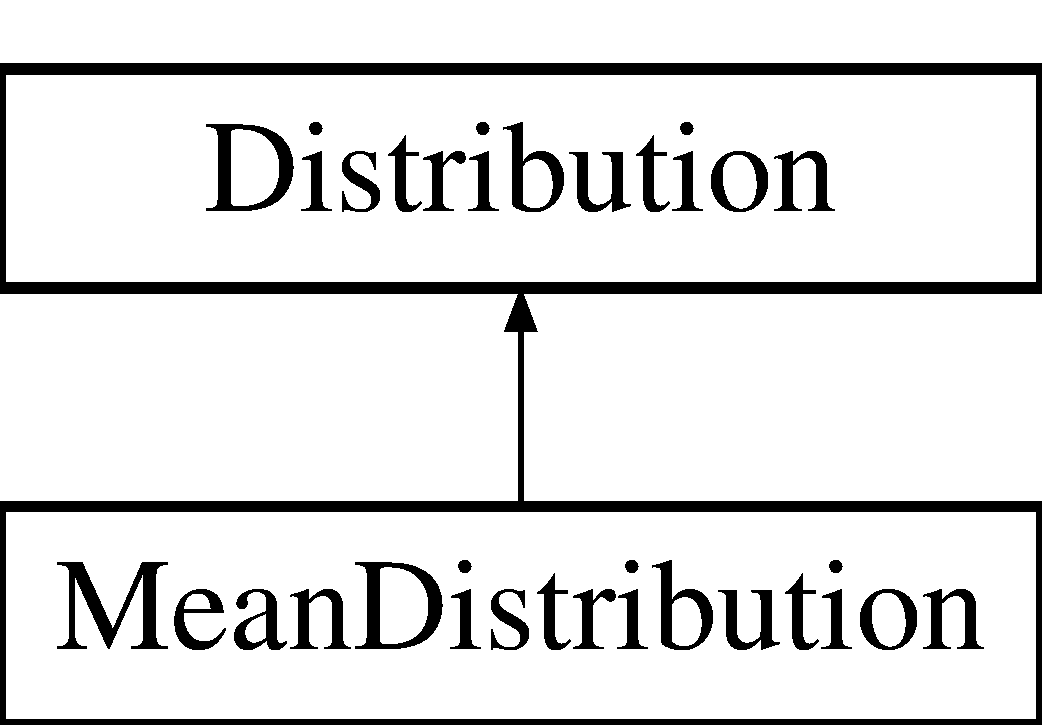
\includegraphics[height=2.000000cm]{classMeanDistribution}
\end{center}
\end{figure}
\subsection*{Public Member Functions}
\begin{DoxyCompactItemize}
\item 
\hypertarget{classMeanDistribution_a4cf60c5fcc4da56771b9e62395c89b2f}{}{\bfseries Mean\+Distribution} (\hyperlink{classHistArray}{Hist\+Array} $\ast$hist, O\+B\+S\+Fnc fnc, O\+B\+S\+Fnc fnc\+\_\+mean)\label{classMeanDistribution_a4cf60c5fcc4da56771b9e62395c89b2f}

\item 
double \hyperlink{classMeanDistribution_ad4b5ab2430e53e5f19c7819d1ae52e02}{Avg} (const \hyperlink{classPS__2}{P\+S\+\_\+2} $\ast$ps)
\begin{DoxyCompactList}\small\item\em Evaluate the observable at the given phase space point. \end{DoxyCompactList}\item 
void \hyperlink{classMeanDistribution_a46b191391f291a6a2b169e52fdf06c23}{Fill} (const \hyperlink{classPS__2}{P\+S\+\_\+2} $\ast$ps)
\begin{DoxyCompactList}\small\item\em Fill histograms with data obtained from the P\+S object. \end{DoxyCompactList}\end{DoxyCompactItemize}


\subsection{Detailed Description}
Class for differential distributions of mean values. 

The mean distribution is an extension of the distribution class. It stores a pointer to a second observable function (O\+B\+S\+Fnc). The class serves to compute distributions of the mean value of this second observable. \begin{DoxySeeAlso}{See also}
\hyperlink{PhaseSpace_8h}{Phase\+Space.\+h} 
\end{DoxySeeAlso}


Definition at line 355 of file Hist\+Array.\+h.



\subsection{Member Function Documentation}
\hypertarget{classMeanDistribution_ad4b5ab2430e53e5f19c7819d1ae52e02}{}\index{Mean\+Distribution@{Mean\+Distribution}!Avg@{Avg}}
\index{Avg@{Avg}!Mean\+Distribution@{Mean\+Distribution}}
\subsubsection[{Avg}]{\setlength{\rightskip}{0pt plus 5cm}double Mean\+Distribution\+::\+Avg (
\begin{DoxyParamCaption}
\item[{const {\bf P\+S\+\_\+2} $\ast$}]{ps}
\end{DoxyParamCaption}
)\hspace{0.3cm}{\ttfamily [inline]}, {\ttfamily [virtual]}}\label{classMeanDistribution_ad4b5ab2430e53e5f19c7819d1ae52e02}


Evaluate the observable at the given phase space point. 


\begin{DoxyParams}{Parameters}
{\em ps} & Phase space point \\
\hline
\end{DoxyParams}


Reimplemented from \hyperlink{classDistribution}{Distribution}.



Definition at line 372 of file Hist\+Array.\+h.

\hypertarget{classMeanDistribution_a46b191391f291a6a2b169e52fdf06c23}{}\index{Mean\+Distribution@{Mean\+Distribution}!Fill@{Fill}}
\index{Fill@{Fill}!Mean\+Distribution@{Mean\+Distribution}}
\subsubsection[{Fill}]{\setlength{\rightskip}{0pt plus 5cm}void Mean\+Distribution\+::\+Fill (
\begin{DoxyParamCaption}
\item[{const {\bf P\+S\+\_\+2} $\ast$}]{ps}
\end{DoxyParamCaption}
)\hspace{0.3cm}{\ttfamily [virtual]}}\label{classMeanDistribution_a46b191391f291a6a2b169e52fdf06c23}


Fill histograms with data obtained from the P\+S object. 


\begin{DoxyParams}{Parameters}
{\em ps} & Phase space object \\
\hline
\end{DoxyParams}


Reimplemented from \hyperlink{classDistribution_a3a1c16200b22ed7253b1b9f50145ebc9}{Distribution}.



The documentation for this class was generated from the following file\+:\begin{DoxyCompactItemize}
\item 
inc/\hyperlink{HistArray_8h}{Hist\+Array.\+h}\end{DoxyCompactItemize}

\hypertarget{structopt}{\section{opt Struct Reference}
\label{structopt}\index{opt@{opt}}
}
\subsection*{Public Attributes}
\begin{DoxyCompactItemize}
\item 
\hypertarget{structopt_acc52d812132128f6088537b4e7e07be6}{int {\bfseries int\-\_\-flags}}\label{structopt_acc52d812132128f6088537b4e7e07be6}

\item 
\hypertarget{structopt_a6ddc969cea0f437ecea3bb299d14f69d}{int {\bfseries n\-\_\-calls}}\label{structopt_a6ddc969cea0f437ecea3bb299d14f69d}

\item 
\hypertarget{structopt_a076fcc87cf2c8ce62c9504c304015d45}{double {\bfseries ren\-\_\-scale}}\label{structopt_a076fcc87cf2c8ce62c9504c304015d45}

\item 
\hypertarget{structopt_a8f98480b8d9fd189e551b50bf7b0e87d}{double {\bfseries cme}}\label{structopt_a8f98480b8d9fd189e551b50bf7b0e87d}

\item 
\hypertarget{structopt_ad1b957514a9167bd98702fe28164d8b0}{double {\bfseries m\-H}}\label{structopt_ad1b957514a9167bd98702fe28164d8b0}

\item 
\hypertarget{structopt_a16156d318278444ca198e3ce8ce0d2f5}{double {\bfseries Gamma\-H}}\label{structopt_a16156d318278444ca198e3ce8ce0d2f5}

\item 
\hypertarget{structopt_a6eff22383bb8bd0d4102be7f449e9d3e}{double {\bfseries At}}\label{structopt_a6eff22383bb8bd0d4102be7f449e9d3e}

\item 
\hypertarget{structopt_a92ea7532f4697352c6651bab251afcf6}{double {\bfseries Bt}}\label{structopt_a92ea7532f4697352c6651bab251afcf6}

\item 
\hypertarget{structopt_a40966817c4ab35a1c2971874b4d013f1}{double {\bfseries Ab}}\label{structopt_a40966817c4ab35a1c2971874b4d013f1}

\item 
\hypertarget{structopt_ae47eb63b3b7691d38d07e9e79ef7de0f}{double {\bfseries Bb}}\label{structopt_ae47eb63b3b7691d38d07e9e79ef7de0f}

\item 
\hypertarget{structopt_aced2f60b766a42008f9da934cef2f540}{int {\bfseries tech\-\_\-cut}}\label{structopt_aced2f60b766a42008f9da934cef2f540}

\item 
\hypertarget{structopt_ad36cc92ecbf8b2bc1deabde5268e9267}{int {\bfseries precision}}\label{structopt_ad36cc92ecbf8b2bc1deabde5268e9267}

\item 
\hypertarget{structopt_acd1b95ec5257a323cd3eb454c7ccd885}{bool {\bfseries dist}}\label{structopt_acd1b95ec5257a323cd3eb454c7ccd885}

\item 
\hypertarget{structopt_aedbcd7fea16a0fa968a1d75884fc0a4c}{bool {\bfseries tdecay}}\label{structopt_aedbcd7fea16a0fa968a1d75884fc0a4c}

\item 
\hypertarget{structopt_af0867351f5c3fd59d3cc5136cf423fc9}{bool {\bfseries logfile}}\label{structopt_af0867351f5c3fd59d3cc5136cf423fc9}

\item 
\hypertarget{structopt_a8d7af1ad473a324bd3633c7ef412c3fc}{bool {\bfseries rootfile}}\label{structopt_a8d7af1ad473a324bd3633c7ef412c3fc}

\item 
\hypertarget{structopt_abe0f9e730fd8eb6b107169359c859a3d}{int {\bfseries verb\-\_\-level}}\label{structopt_abe0f9e730fd8eb6b107169359c859a3d}

\end{DoxyCompactItemize}


\subsection{Detailed Description}


Definition at line 50 of file Functions\-\_\-\-Shared.\-h.



The documentation for this struct was generated from the following file\-:\begin{DoxyCompactItemize}
\item 
inc/Functions\-\_\-\-Shared.\-h\end{DoxyCompactItemize}

\hypertarget{classPS__2}{}\section{P\+S\+\_\+2 Class Reference}
\label{classPS__2}\index{P\+S\+\_\+2@{P\+S\+\_\+2}}


Abstract base class for 2-\/$>$X phase space classes.  




{\ttfamily \#include $<$Phase\+Space.\+h$>$}

Inheritance diagram for P\+S\+\_\+2\+:\begin{figure}[H]
\begin{center}
\leavevmode
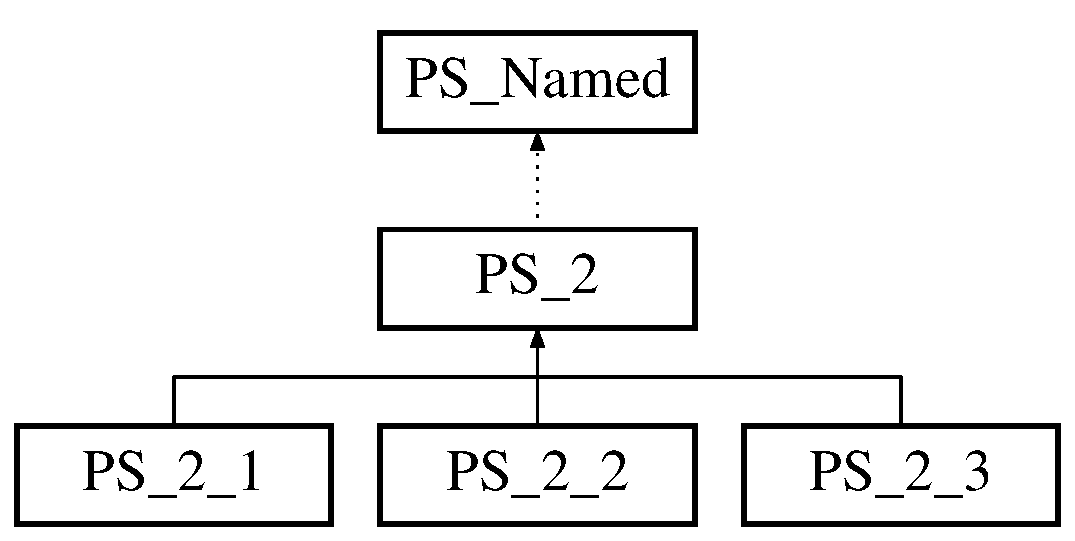
\includegraphics[height=3.000000cm]{classPS__2}
\end{center}
\end{figure}
\subsection*{Public Member Functions}
\begin{DoxyCompactItemize}
\item 
\hypertarget{classPS__2_ae359831d133d3a4830c3600fa8d32c06}{}{\bfseries P\+S\+\_\+2} (const std\+::string \&nm=\char`\"{}\char`\"{})\label{classPS__2_ae359831d133d3a4830c3600fa8d32c06}

\item 
\hypertarget{classPS__2_a8d77fbe890b80085027ac929c85cca18}{}\hyperlink{classFV}{F\+V} \& \hyperlink{classPS__2_a8d77fbe890b80085027ac929c85cca18}{p1} ()\label{classPS__2_a8d77fbe890b80085027ac929c85cca18}

\begin{DoxyCompactList}\small\item\em read/write access to first incoming parton 4-\/momentum \end{DoxyCompactList}\item 
\hypertarget{classPS__2_a51fe8ffc84f4527f5da4530269bc3434}{}\hyperlink{classFV}{F\+V} \& \hyperlink{classPS__2_a51fe8ffc84f4527f5da4530269bc3434}{p2} ()\label{classPS__2_a51fe8ffc84f4527f5da4530269bc3434}

\begin{DoxyCompactList}\small\item\em read/write access to second incoming parton 4-\/momentum \end{DoxyCompactList}\item 
\hypertarget{classPS__2_a999fae525d845b24359f69c99d3f5f67}{}\hyperlink{classFV}{F\+V} const \& \hyperlink{classPS__2_a999fae525d845b24359f69c99d3f5f67}{p1} () const \label{classPS__2_a999fae525d845b24359f69c99d3f5f67}

\begin{DoxyCompactList}\small\item\em read only access to first incoming parton 4-\/momentum \end{DoxyCompactList}\item 
\hypertarget{classPS__2_a144b72cd5af27d3cee36a2d6d88bbb1b}{}\hyperlink{classFV}{F\+V} const \& \hyperlink{classPS__2_a144b72cd5af27d3cee36a2d6d88bbb1b}{p2} () const \label{classPS__2_a144b72cd5af27d3cee36a2d6d88bbb1b}

\begin{DoxyCompactList}\small\item\em read only access to second incoming parton 4-\/momentum \end{DoxyCompactList}\item 
\hypertarget{classPS__2_a44e3773e7808eff87c2db0d1a2244477}{}\hyperlink{classFV}{F\+V} \& \hyperlink{classPS__2_a44e3773e7808eff87c2db0d1a2244477}{P1} ()\label{classPS__2_a44e3773e7808eff87c2db0d1a2244477}

\begin{DoxyCompactList}\small\item\em read/write access to first proton 4-\/momentum \end{DoxyCompactList}\item 
\hypertarget{classPS__2_a67fac165db2b49e4469787c6df78cb62}{}\hyperlink{classFV}{F\+V} \& \hyperlink{classPS__2_a67fac165db2b49e4469787c6df78cb62}{P2} ()\label{classPS__2_a67fac165db2b49e4469787c6df78cb62}

\begin{DoxyCompactList}\small\item\em read/write access to second proton 4-\/momentum \end{DoxyCompactList}\item 
\hypertarget{classPS__2_a772e6e3ed309f0afd1a4676b5cd2df92}{}\hyperlink{classFV}{F\+V} const \& \hyperlink{classPS__2_a772e6e3ed309f0afd1a4676b5cd2df92}{P1} () const \label{classPS__2_a772e6e3ed309f0afd1a4676b5cd2df92}

\begin{DoxyCompactList}\small\item\em read only access to first proton 4-\/momentum \end{DoxyCompactList}\item 
\hypertarget{classPS__2_aa9edfae86df81b545e27926fe7318e3e}{}\hyperlink{classFV}{F\+V} const \& \hyperlink{classPS__2_aa9edfae86df81b545e27926fe7318e3e}{P2} () const \label{classPS__2_aa9edfae86df81b545e27926fe7318e3e}

\begin{DoxyCompactList}\small\item\em read only access to second proton 4-\/momentum \end{DoxyCompactList}\item 
\hypertarget{classPS__2_a77b7be40d4f31c23a0bb0c112669c637}{}double const \& {\bfseries get\+\_\+rs} () const \label{classPS__2_a77b7be40d4f31c23a0bb0c112669c637}

\item 
\hypertarget{classPS__2_a3ef9ac96876f61f0c6a46a5321107bee}{}double {\bfseries get\+\_\+s} () const \label{classPS__2_a3ef9ac96876f61f0c6a46a5321107bee}

\item 
\hypertarget{classPS__2_a3b361fd3b41b8b92ab98e44dee130af8}{}void {\bfseries set\+\_\+rs} (double const \&rs)\label{classPS__2_a3b361fd3b41b8b92ab98e44dee130af8}

\item 
\hypertarget{classPS__2_a5063384c1c8b5e500f33970c01712f59}{}bool \hyperlink{classPS__2_a5063384c1c8b5e500f33970c01712f59}{toggle\+\_\+decay} ()\label{classPS__2_a5063384c1c8b5e500f33970c01712f59}

\begin{DoxyCompactList}\small\item\em not used \end{DoxyCompactList}\item 
\hypertarget{classPS__2_a049e0480c37ac84a8319f19bcfb335ab}{}double const \& \hyperlink{classPS__2_a049e0480c37ac84a8319f19bcfb335ab}{get\+\_\+wgt} ()\label{classPS__2_a049e0480c37ac84a8319f19bcfb335ab}

\begin{DoxyCompactList}\small\item\em get current phase space weight \end{DoxyCompactList}\item 
\hypertarget{classPS__2_a743942dc8d537cfed9d229aad62aa96a}{}int {\bfseries set\+\_\+parent} (\hyperlink{classPS__2}{P\+S\+\_\+2} $\ast$parent)\label{classPS__2_a743942dc8d537cfed9d229aad62aa96a}

\item 
\hypertarget{classPS__2_afefab6481fa7a0dde6ddc5a1f8d1642f}{}void \hyperlink{classPS__2_afefab6481fa7a0dde6ddc5a1f8d1642f}{swap\+\_\+initial\+\_\+state} ()\label{classPS__2_afefab6481fa7a0dde6ddc5a1f8d1642f}

\begin{DoxyCompactList}\small\item\em swap incoming parton and proton momenta \end{DoxyCompactList}\item 
\hypertarget{classPS__2_a5865322be9736bf043cc8bd1d5127a52}{}virtual double const \& {\bfseries get\+\_\+msq} (int i) const =0\label{classPS__2_a5865322be9736bf043cc8bd1d5127a52}

\item 
\hypertarget{classPS__2_af44e67d84bc53b126d720907adeaffc2}{}virtual \hyperlink{classPS__2}{P\+S\+\_\+2} $\ast$ {\bfseries get\+\_\+child} (int i) const =0\label{classPS__2_af44e67d84bc53b126d720907adeaffc2}

\item 
\hypertarget{classPS__2_a74d62c9ae71d30741838408fabaf4ba3}{}virtual int {\bfseries set\+\_\+child} (int i, \hyperlink{classPS__2}{P\+S\+\_\+2} $\ast$child)=0\label{classPS__2_a74d62c9ae71d30741838408fabaf4ba3}

\item 
\hypertarget{classPS__2_aa23e50a0b5d3ac32fb63afb4f67d3910}{}virtual \hyperlink{classFV}{F\+V} const \& {\bfseries get\+\_\+k} (int i) const =0\label{classPS__2_aa23e50a0b5d3ac32fb63afb4f67d3910}

\item 
\hypertarget{classPS__2_ac3bb7468d7b1e1b62018f13a1121e86a}{}virtual int {\bfseries whattype} () const =0\label{classPS__2_ac3bb7468d7b1e1b62018f13a1121e86a}

\item 
\hypertarget{classPS__2_a395f9455cfdebcfd145ba679c43ac2c5}{}virtual void {\bfseries print} () const \label{classPS__2_a395f9455cfdebcfd145ba679c43ac2c5}

\item 
\hypertarget{classPS__2_a1a073b4fd3fafa46dceabcf77f4b3c44}{}virtual \hyperlink{classFV}{F\+V} const \& {\bfseries k1} () const \label{classPS__2_a1a073b4fd3fafa46dceabcf77f4b3c44}

\item 
\hypertarget{classPS__2_a9caf1d80ebd0718a226e05bf42cfa4c9}{}virtual \hyperlink{classFV}{F\+V} const \& {\bfseries k2} () const \label{classPS__2_a9caf1d80ebd0718a226e05bf42cfa4c9}

\item 
\hypertarget{classPS__2_aaa94aa598e69a134fab3bc2fc6c3185b}{}virtual \hyperlink{classFV}{F\+V} const \& {\bfseries k3} () const \label{classPS__2_aaa94aa598e69a134fab3bc2fc6c3185b}

\end{DoxyCompactItemize}
\subsection*{Static Public Attributes}
\begin{DoxyCompactItemize}
\item 
\hypertarget{classPS__2_af361ee1bfe02e206f8845db7f1da57c6}{}static const \hyperlink{classFV}{F\+V} {\bfseries nullvec}\label{classPS__2_af361ee1bfe02e206f8845db7f1da57c6}

\end{DoxyCompactItemize}
\subsection*{Protected Member Functions}
\begin{DoxyCompactItemize}
\item 
\hypertarget{classPS__2_a6d49cef4b1eb1138b947c9ec9b448538}{}void {\bfseries set\+\_\+initial\+\_\+state} (double const \&s)\label{classPS__2_a6d49cef4b1eb1138b947c9ec9b448538}

\end{DoxyCompactItemize}
\subsection*{Protected Attributes}
\begin{DoxyCompactItemize}
\item 
\hypertarget{classPS__2_a20ee7f6afb71183f2f61c7049b2e1c9e}{}double \hyperlink{classPS__2_a20ee7f6afb71183f2f61c7049b2e1c9e}{d\+\_\+rs}\label{classPS__2_a20ee7f6afb71183f2f61c7049b2e1c9e}

\begin{DoxyCompactList}\small\item\em square root of the current partonic c.\+m.\+e. \end{DoxyCompactList}\item 
\hypertarget{classPS__2_ac717630d614c3bce592b1d0ba1d969c7}{}\hyperlink{classFV}{F\+V} \hyperlink{classPS__2_ac717630d614c3bce592b1d0ba1d969c7}{p} \mbox{[}2\mbox{]}\label{classPS__2_ac717630d614c3bce592b1d0ba1d969c7}

\begin{DoxyCompactList}\small\item\em incoming parton 4-\/momenta \end{DoxyCompactList}\item 
\hypertarget{classPS__2_a9c8c1bd53ef9086e96705be1377564ec}{}\hyperlink{classFV}{F\+V} \hyperlink{classPS__2_a9c8c1bd53ef9086e96705be1377564ec}{P} \mbox{[}2\mbox{]}\label{classPS__2_a9c8c1bd53ef9086e96705be1377564ec}

\begin{DoxyCompactList}\small\item\em incoming proton 4-\/momenta, used to define the boost that connects parton z.\+m.\+f. and lab frame \end{DoxyCompactList}\item 
\hypertarget{classPS__2_a7840687732819d92810f9a2666621650}{}double \hyperlink{classPS__2_a7840687732819d92810f9a2666621650}{d\+\_\+wgt}\label{classPS__2_a7840687732819d92810f9a2666621650}

\begin{DoxyCompactList}\small\item\em current phase space density \end{DoxyCompactList}\item 
\hypertarget{classPS__2_a973be656af67bb3516424e664a49ae55}{}bool \hyperlink{classPS__2_a973be656af67bb3516424e664a49ae55}{d\+\_\+decay}\label{classPS__2_a973be656af67bb3516424e664a49ae55}

\begin{DoxyCompactList}\small\item\em not used \end{DoxyCompactList}\item 
\hypertarget{classPS__2_abebb860c3c4a1c5054bc223d3aac4f45}{}\hyperlink{classPS__2}{P\+S\+\_\+2} $\ast$ \hyperlink{classPS__2_abebb860c3c4a1c5054bc223d3aac4f45}{d\+\_\+parent}\label{classPS__2_abebb860c3c4a1c5054bc223d3aac4f45}

\begin{DoxyCompactList}\small\item\em pointer to parent P\+S instance, used to combine phase spaces 2-\/$>$i + 2-\/$>$j = 2-\/$>$i+j-\/1 \end{DoxyCompactList}\end{DoxyCompactItemize}


\subsection{Detailed Description}
Abstract base class for 2-\/$>$X phase space classes. 

Holds among others the 4-\/vectors of the incoming partons. \begin{DoxySeeAlso}{See also}
\hyperlink{Lorentz_8h}{Lorentz.\+h}, \hyperlink{HistArray_8h}{Hist\+Array.\+h} 
\end{DoxySeeAlso}


Definition at line 56 of file Phase\+Space.\+h.



The documentation for this class was generated from the following files\+:\begin{DoxyCompactItemize}
\item 
inc/\hyperlink{PhaseSpace_8h}{Phase\+Space.\+h}\item 
src/Phase\+Space.\+cpp\end{DoxyCompactItemize}

\hypertarget{classPS__2__1}{}\section{P\+S\+\_\+2\+\_\+1 Class Reference}
\label{classPS__2__1}\index{P\+S\+\_\+2\+\_\+1@{P\+S\+\_\+2\+\_\+1}}


{\ttfamily \#include $<$Phase\+Space.\+h$>$}

Inheritance diagram for P\+S\+\_\+2\+\_\+1\+:\begin{figure}[H]
\begin{center}
\leavevmode
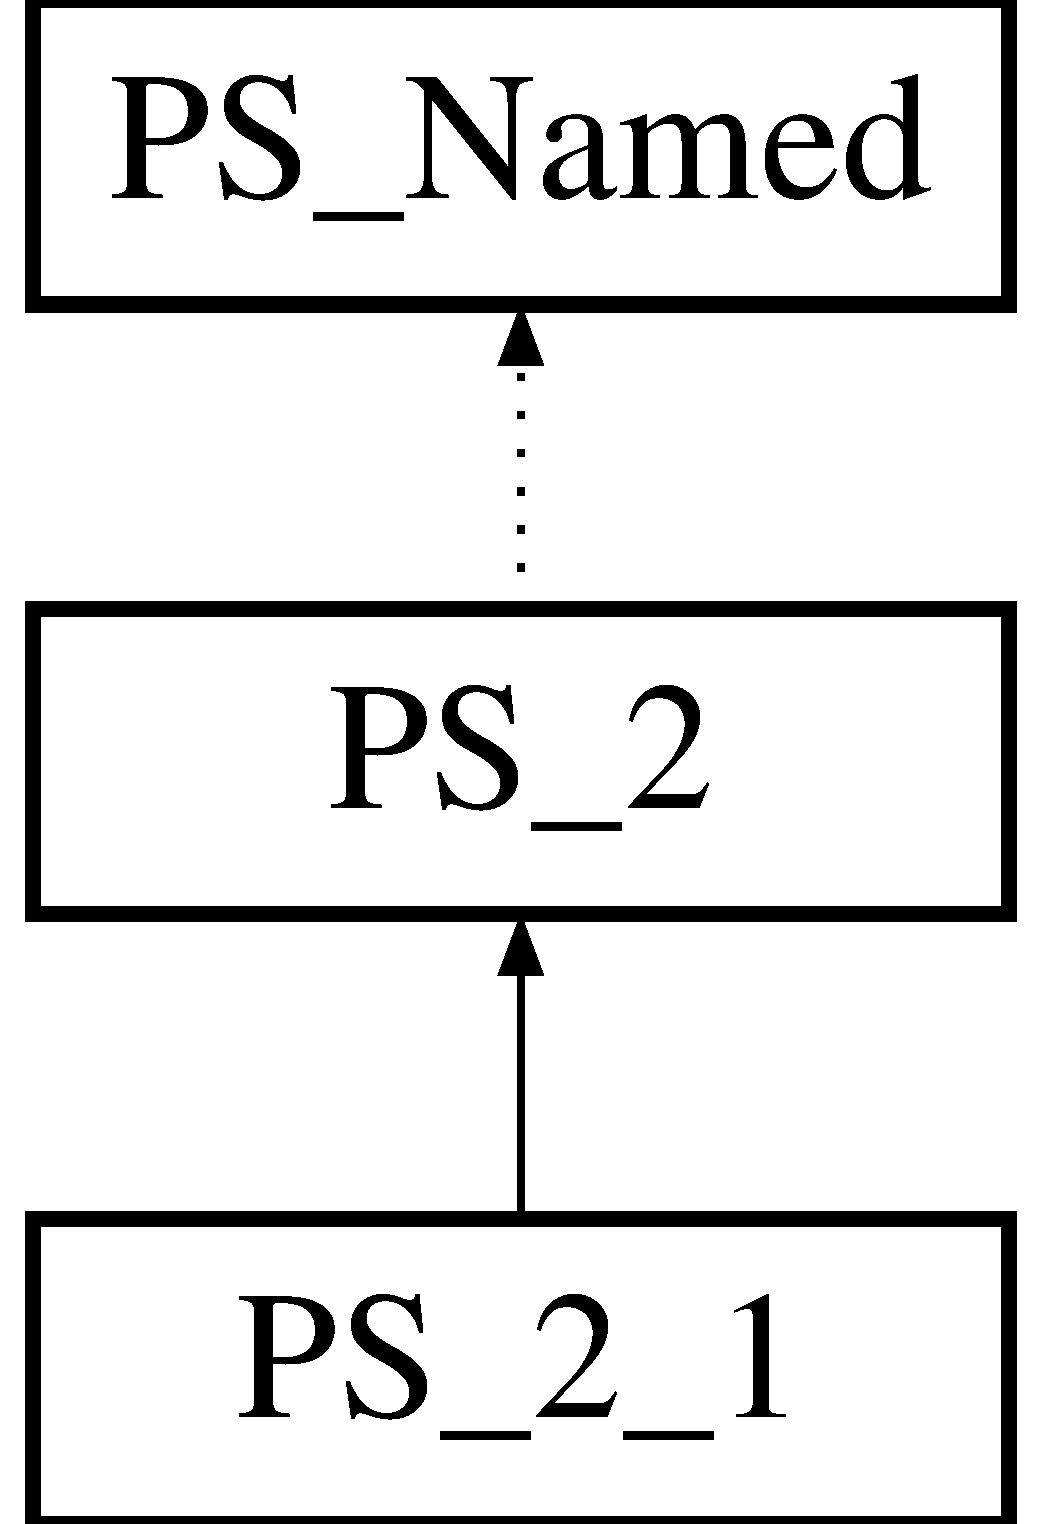
\includegraphics[height=3.000000cm]{classPS__2__1}
\end{center}
\end{figure}
\subsection*{Public Member Functions}
\begin{DoxyCompactItemize}
\item 
\hypertarget{classPS__2__1_abdf4e57ac00768c463aa0f25ca8eaa55}{}{\bfseries P\+S\+\_\+2\+\_\+1} (const std\+::string \&nm=\char`\"{}2-\/$>$2\char`\"{})\label{classPS__2__1_abdf4e57ac00768c463aa0f25ca8eaa55}

\item 
\hypertarget{classPS__2__1_a5f6b4ede135f7decfad67cafa2be6a1f}{}{\bfseries P\+S\+\_\+2\+\_\+1} (double const \&msq, const std\+::string \&nm=\char`\"{}2-\/$>$2\char`\"{})\label{classPS__2__1_a5f6b4ede135f7decfad67cafa2be6a1f}

\item 
\hypertarget{classPS__2__1_a85f554f63cdd77eb9e961f21dc8a5025}{}void {\bfseries set\+\_\+x} (double const \&x)\label{classPS__2__1_a85f554f63cdd77eb9e961f21dc8a5025}

\item 
\hypertarget{classPS__2__1_ae61b15b9a11d358ab1db760a68d29a48}{}double const \& {\bfseries get\+\_\+x} () const \label{classPS__2__1_ae61b15b9a11d358ab1db760a68d29a48}

\item 
\hypertarget{classPS__2__1_ad6834a4e1e1b0e7081020d9c93fce803}{}\hyperlink{classFV}{F\+V} const \& {\bfseries get\+\_\+k} (int i) const \label{classPS__2__1_ad6834a4e1e1b0e7081020d9c93fce803}

\item 
\hypertarget{classPS__2__1_ac47a7de9d93c165993b96aeb6d8b51a9}{}\hyperlink{classPS__2}{P\+S\+\_\+2} $\ast$ {\bfseries get\+\_\+child} (int i) const \label{classPS__2__1_ac47a7de9d93c165993b96aeb6d8b51a9}

\item 
\hypertarget{classPS__2__1_ac1ebcf6777ab799e9c56f90ec6bd0d63}{}double const \& {\bfseries get\+\_\+msq} (int i) const \label{classPS__2__1_ac1ebcf6777ab799e9c56f90ec6bd0d63}

\item 
\hypertarget{classPS__2__1_ad3a493e3ccbb2b98c6e74131ba62d840}{}void {\bfseries set\+\_\+msq} (double const \&msq)\label{classPS__2__1_ad3a493e3ccbb2b98c6e74131ba62d840}

\item 
\hypertarget{classPS__2__1_a0c349c6d76745bf8c345b6193b4a382a}{}\hyperlink{classFV}{F\+V} \& {\bfseries k1} ()\label{classPS__2__1_a0c349c6d76745bf8c345b6193b4a382a}

\item 
\hypertarget{classPS__2__1_a8896fae62d323bceb002628a95466f3f}{}\hyperlink{classFV}{F\+V} const \& {\bfseries k1} () const \label{classPS__2__1_a8896fae62d323bceb002628a95466f3f}

\item 
\hypertarget{classPS__2__1_a02e613ae4acac6c2ea9c57a49a8e3f68}{}int {\bfseries set} ()\label{classPS__2__1_a02e613ae4acac6c2ea9c57a49a8e3f68}

\item 
\hypertarget{classPS__2__1_a3bcae5991298ad9a2fc143d4461c60fa}{}int {\bfseries set\+\_\+child} (int i, \hyperlink{classPS__2}{P\+S\+\_\+2} $\ast$child)\label{classPS__2__1_a3bcae5991298ad9a2fc143d4461c60fa}

\item 
\hypertarget{classPS__2__1_aaa0d8ed0b5e2673cb5f2cd84f090e1f9}{}int {\bfseries whattype} () const \label{classPS__2__1_aaa0d8ed0b5e2673cb5f2cd84f090e1f9}

\item 
\hypertarget{classPS__2__1_a21760964ae4b35c2cfeff16b4c569c3a}{}void {\bfseries print} () const \label{classPS__2__1_a21760964ae4b35c2cfeff16b4c569c3a}

\item 
void \hyperlink{classPS__2__1_a5cf9231c96cfcb45b3b5dbf6646f68f3}{Fill\+Distributions} (Dist\+Vec \&dist, H\+\_\+\+I\+N\+D\+E\+X id, double const \&wgt, double const \&m\+Scale=1.\+0) const 
\end{DoxyCompactItemize}
\subsection*{Protected Attributes}
\begin{DoxyCompactItemize}
\item 
\hypertarget{classPS__2__1_a3606766aee8e4775462c15adda3acbc5}{}\hyperlink{classFV}{F\+V} {\bfseries k}\label{classPS__2__1_a3606766aee8e4775462c15adda3acbc5}

\item 
\hypertarget{classPS__2__1_a415b225aedab250a67aee39ef0d859bc}{}double {\bfseries d\+\_\+msq}\label{classPS__2__1_a415b225aedab250a67aee39ef0d859bc}

\item 
\hypertarget{classPS__2__1_a015027e1fc8e30949ea8a439cfedddd4}{}\hyperlink{classPS__2}{P\+S\+\_\+2} $\ast$ {\bfseries d\+\_\+child}\label{classPS__2__1_a015027e1fc8e30949ea8a439cfedddd4}

\item 
\hypertarget{classPS__2__1_af18aa8f6679b7ac65be236b00e794e0c}{}double {\bfseries d\+\_\+x}\label{classPS__2__1_af18aa8f6679b7ac65be236b00e794e0c}

\end{DoxyCompactItemize}
\subsection*{Additional Inherited Members}


\subsection{Detailed Description}
Phase space for 2-\/$>$1 scattering. 

Definition at line 145 of file Phase\+Space.\+h.



\subsection{Member Function Documentation}
\hypertarget{classPS__2__1_a5cf9231c96cfcb45b3b5dbf6646f68f3}{}\index{P\+S\+\_\+2\+\_\+1@{P\+S\+\_\+2\+\_\+1}!Fill\+Distributions@{Fill\+Distributions}}
\index{Fill\+Distributions@{Fill\+Distributions}!P\+S\+\_\+2\+\_\+1@{P\+S\+\_\+2\+\_\+1}}
\subsubsection[{Fill\+Distributions}]{\setlength{\rightskip}{0pt plus 5cm}void P\+S\+\_\+2\+\_\+1\+::\+Fill\+Distributions (
\begin{DoxyParamCaption}
\item[{Dist\+Vec \&}]{dist, }
\item[{H\+\_\+\+I\+N\+D\+E\+X}]{id, }
\item[{double const \&}]{wgt, }
\item[{double const \&}]{m\+Scale = {\ttfamily 1.0}}
\end{DoxyParamCaption}
) const}\label{classPS__2__1_a5cf9231c96cfcb45b3b5dbf6646f68f3}
Feed the distributions in the vector \textquotesingle{}dist\textquotesingle{} with the weight \textquotesingle{}wgt\textquotesingle{} in the bin corresponding to their observable evaluated at the current point of this phase space object. N\+O\+T Y\+E\+T I\+M\+P\+L\+E\+M\+E\+N\+T\+E\+D O\+N \hyperlink{classPS__2__1}{P\+S\+\_\+2\+\_\+1} !!! 
\begin{DoxyParams}{Parameters}
{\em dist} & Vector of distributions. \\
\hline
{\em id} & Fill into this histogram in each \hyperlink{classHistArray}{Hist\+Array}. \\
\hline
{\em wgt} & Weigth to dill into the distributions. \\
\hline
{\em m\+Scale} & Mass scale used for normalization. Necessary to get the correct numerical values of the observables with non-\/zero mass dimension. \\
\hline
\end{DoxyParams}


Definition at line 105 of file Phase\+Space.\+cpp.



The documentation for this class was generated from the following files\+:\begin{DoxyCompactItemize}
\item 
inc/\hyperlink{PhaseSpace_8h}{Phase\+Space.\+h}\item 
src/Phase\+Space.\+cpp\end{DoxyCompactItemize}

\hypertarget{classPS__2__2}{}\section{P\+S\+\_\+2\+\_\+2 Class Reference}
\label{classPS__2__2}\index{P\+S\+\_\+2\+\_\+2@{P\+S\+\_\+2\+\_\+2}}


Phase space for 2-\/$>$2 scattering.  




{\ttfamily \#include $<$Phase\+Space.\+h$>$}

Inheritance diagram for P\+S\+\_\+2\+\_\+2\+:\begin{figure}[H]
\begin{center}
\leavevmode
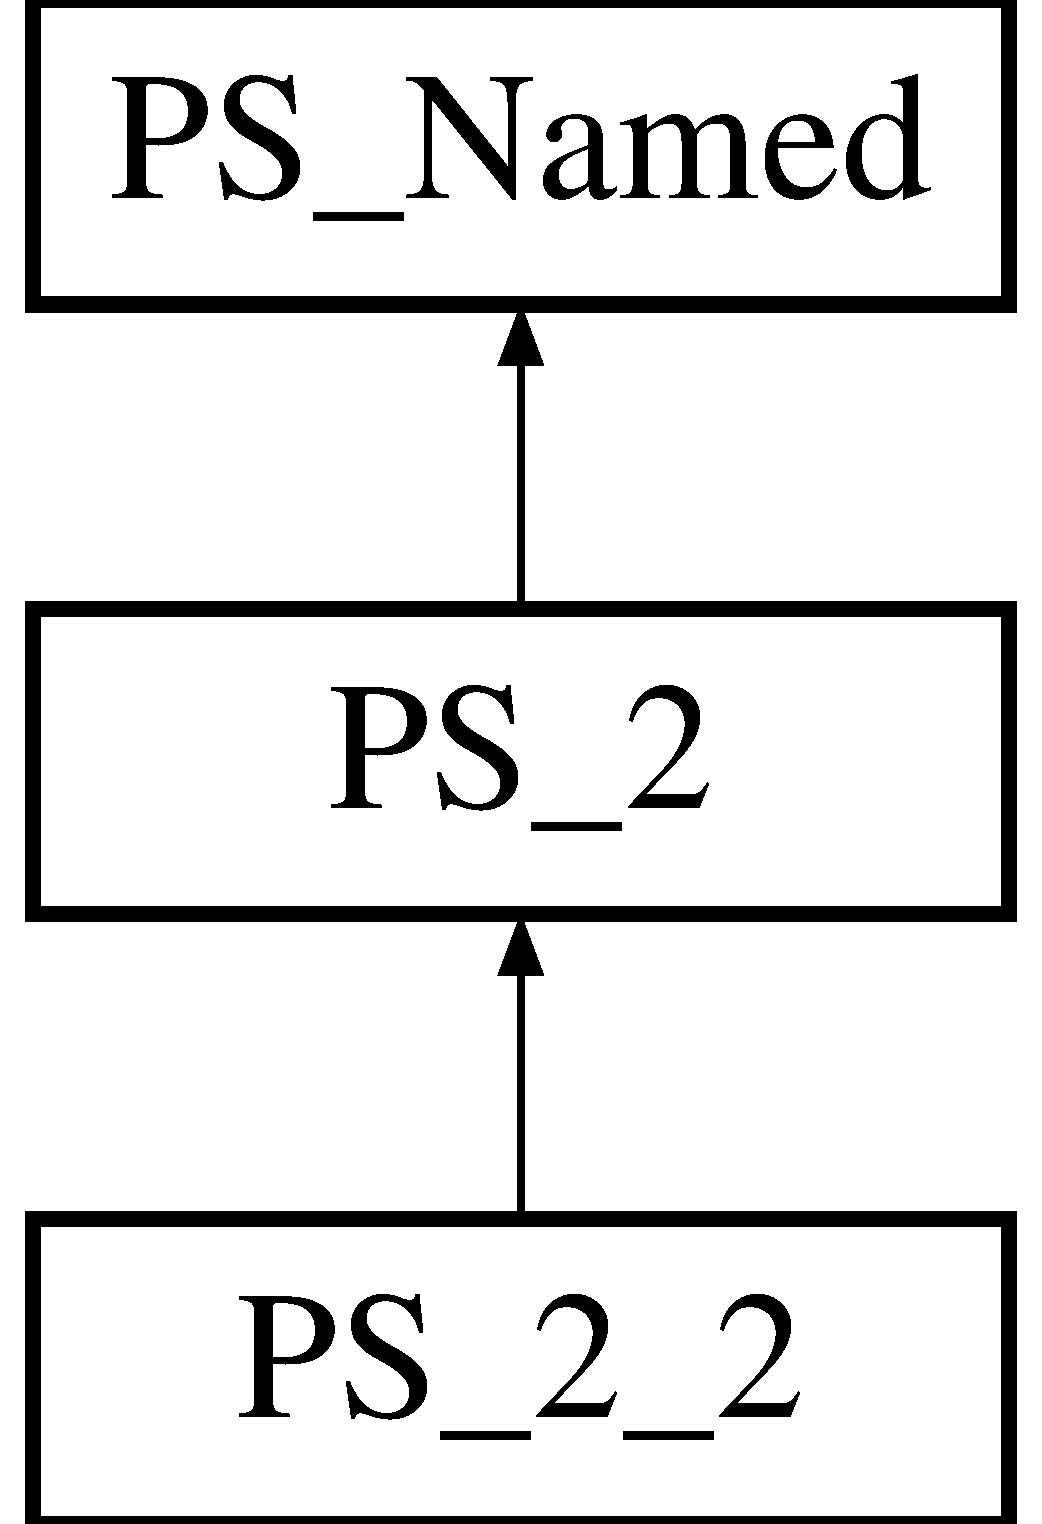
\includegraphics[height=3.000000cm]{classPS__2__2}
\end{center}
\end{figure}
\subsection*{Public Member Functions}
\begin{DoxyCompactItemize}
\item 
\hypertarget{classPS__2__2_a2c69fba98e2519e9247f8052b642dcdc}{}{\bfseries P\+S\+\_\+2\+\_\+2} (const std\+::string \&nm=\char`\"{}2-\/$>$2\char`\"{})\label{classPS__2__2_a2c69fba98e2519e9247f8052b642dcdc}

\item 
\hypertarget{classPS__2__2_a9656aed0fb1409f829f84f1c568ced85}{}{\bfseries P\+S\+\_\+2\+\_\+2} (double const \&m1sq, double const \&m2sq, const std\+::string \&nm=\char`\"{}2-\/$>$2\char`\"{})\label{classPS__2__2_a9656aed0fb1409f829f84f1c568ced85}

\item 
\hypertarget{classPS__2__2_a27f5570839ad56e039feb1b693c47fc4}{}\hyperlink{classFV}{F\+V} const \& {\bfseries get\+\_\+k} (int i) const \label{classPS__2__2_a27f5570839ad56e039feb1b693c47fc4}

\item 
\hypertarget{classPS__2__2_a75fb8afaac5a5feb3f914fd0bfbcc7b3}{}\hyperlink{classPS__2}{P\+S\+\_\+2} $\ast$ {\bfseries get\+\_\+child} (int i) const \label{classPS__2__2_a75fb8afaac5a5feb3f914fd0bfbcc7b3}

\item 
\hypertarget{classPS__2__2_a038add35c67f07679dea7cb99831296c}{}double const \& {\bfseries get\+\_\+msq} (int i) const \label{classPS__2__2_a038add35c67f07679dea7cb99831296c}

\item 
\hypertarget{classPS__2__2_ae781b2b360acc3f902c91eef23ca1a80}{}void {\bfseries set\+\_\+msq} (double const \&m1sq, double const \&m2sq)\label{classPS__2__2_ae781b2b360acc3f902c91eef23ca1a80}

\item 
\hypertarget{classPS__2__2_a1fff415d89393fe3817d033ca94cddfc}{}double const \& {\bfseries get\+\_\+beta} (int i) const \label{classPS__2__2_a1fff415d89393fe3817d033ca94cddfc}

\item 
\hypertarget{classPS__2__2_accd43c9b6a1ad37cd7730ce42302b2f4}{}double const \& {\bfseries get\+\_\+beta} () const \label{classPS__2__2_accd43c9b6a1ad37cd7730ce42302b2f4}

\item 
\hypertarget{classPS__2__2_a31d25d54497c8dded3c57c117c59dbd6}{}double const \& {\bfseries get\+\_\+y} () const \label{classPS__2__2_a31d25d54497c8dded3c57c117c59dbd6}

\item 
\hypertarget{classPS__2__2_a28bf4d69f8fcb2b359f521289a6a70d1}{}double const \& {\bfseries get\+\_\+phi} () const \label{classPS__2__2_a28bf4d69f8fcb2b359f521289a6a70d1}

\item 
\hypertarget{classPS__2__2_ae717002f8f6d84446f4353aa3cc97757}{}double const \& {\bfseries get\+\_\+t11} () const \label{classPS__2__2_ae717002f8f6d84446f4353aa3cc97757}

\item 
\hypertarget{classPS__2__2_a9e2bc01c150ce569013cebf16ca34528}{}double const \& {\bfseries get\+\_\+t12} () const \label{classPS__2__2_a9e2bc01c150ce569013cebf16ca34528}

\item 
\hypertarget{classPS__2__2_a3b1392c5e6a6e894b87926611333e782}{}double const \& {\bfseries get\+\_\+x} () const \label{classPS__2__2_a3b1392c5e6a6e894b87926611333e782}

\item 
\hypertarget{classPS__2__2_a7c253fa9526fb882c0fb386700f0a084}{}double const \& {\bfseries get\+\_\+beta\+\_\+y} () const \label{classPS__2__2_a7c253fa9526fb882c0fb386700f0a084}

\item 
\hypertarget{classPS__2__2_ab38bb5b8ac36bea7b044a72d0c9cfdbb}{}void {\bfseries set\+\_\+x} (double const \&x)\label{classPS__2__2_ab38bb5b8ac36bea7b044a72d0c9cfdbb}

\item 
\hypertarget{classPS__2__2_ad816da6fba743fbe6d7e67e119ad1cca}{}double \hyperlink{classPS__2__2_ad816da6fba743fbe6d7e67e119ad1cca}{cmp\+\_\+wgt} ()\label{classPS__2__2_ad816da6fba743fbe6d7e67e119ad1cca}

\begin{DoxyCompactList}\small\item\em compute the phase space density for the current setting \end{DoxyCompactList}\item 
\hypertarget{classPS__2__2_a11a23bbf3ce1288121b6f798012039ea}{}\hyperlink{classFV}{F\+V} \& {\bfseries k1} ()\label{classPS__2__2_a11a23bbf3ce1288121b6f798012039ea}

\item 
\hypertarget{classPS__2__2_ae80de8ff0390f3a92cf8cb55bafcfa39}{}\hyperlink{classFV}{F\+V} \& {\bfseries k2} ()\label{classPS__2__2_ae80de8ff0390f3a92cf8cb55bafcfa39}

\item 
\hypertarget{classPS__2__2_a50a2e1f1876ab83fbee307434053f9f5}{}\hyperlink{classFV}{F\+V} const \& {\bfseries k1} () const \label{classPS__2__2_a50a2e1f1876ab83fbee307434053f9f5}

\item 
\hypertarget{classPS__2__2_af926b46a1c778aa2e89e6c21ca7fbe1b}{}\hyperlink{classFV}{F\+V} const \& {\bfseries k2} () const \label{classPS__2__2_af926b46a1c778aa2e89e6c21ca7fbe1b}

\item 
\hypertarget{classPS__2__2_a62103a2d987ed8b04918d584e1c7c562}{}int \hyperlink{classPS__2__2_a62103a2d987ed8b04918d584e1c7c562}{boost\+\_\+initial\+\_\+state} ()\label{classPS__2__2_a62103a2d987ed8b04918d584e1c7c562}

\begin{DoxyCompactList}\small\item\em boost initial state partons by a factor of d\+\_\+x \end{DoxyCompactList}\item 
\hypertarget{classPS__2__2_abdf4c563c0c67169a478fb7719581a35}{}int \hyperlink{classPS__2__2_abdf4c563c0c67169a478fb7719581a35}{boost\+\_\+initial\+\_\+state} (double const \&x)\label{classPS__2__2_abdf4c563c0c67169a478fb7719581a35}

\begin{DoxyCompactList}\small\item\em boost initial state partons by a factor of x \end{DoxyCompactList}\item 
\hypertarget{classPS__2__2_a397211db7a5b9781886cc55dae1d23d3}{}int {\bfseries boost\+\_\+final\+\_\+state} ()\label{classPS__2__2_a397211db7a5b9781886cc55dae1d23d3}

\item 
int \hyperlink{classPS__2__2_add28db38c9779539849ecb4384432911}{set} (double const \&rs, double const \&y, double const \&phi=0.\+0)
\item 
\hypertarget{classPS__2__2_ae66bec7df54e50255d0e3e5d779e0dae}{}int \hyperlink{classPS__2__2_ae66bec7df54e50255d0e3e5d779e0dae}{set} (double const \&x=0.\+0)\label{classPS__2__2_ae66bec7df54e50255d0e3e5d779e0dae}

\begin{DoxyCompactList}\small\item\em New phase space setting\+: compute c.\+m.\+e rs = sqrt(s\+\_\+part) and scattering angles y, phi and all derived quantities from current set of 4-\/vectors. \end{DoxyCompactList}\item 
\hypertarget{classPS__2__2_a7ed4acdee85fea6b129aa9801cb8d3c7}{}int {\bfseries set\+\_\+child} (int i, \hyperlink{classPS__2}{P\+S\+\_\+2} $\ast$child)\label{classPS__2__2_a7ed4acdee85fea6b129aa9801cb8d3c7}

\item 
\hypertarget{classPS__2__2_a27ba82e9c32ba391be7df643181de646}{}int {\bfseries whattype} () const \label{classPS__2__2_a27ba82e9c32ba391be7df643181de646}

\item 
\hypertarget{classPS__2__2_af19d44fe30fb72ccfc20f5626f04dcdc}{}void {\bfseries print} () const \label{classPS__2__2_af19d44fe30fb72ccfc20f5626f04dcdc}

\item 
void \hyperlink{classPS__2__2_a253769d43f0d405d6109d16805a4b0c2}{Fill\+Distributions} (Dist\+Vec \&dist, \hyperlink{HistArray_8h_abdf25c9f0ab78c4243f63cb2bacf26d9}{H\+\_\+\+Index} id, double const \&wgt, double const \&m\+Scale=1.\+0) const 
\end{DoxyCompactItemize}
\subsection*{Additional Inherited Members}


\subsection{Detailed Description}
Phase space for 2-\/$>$2 scattering. 

Definition at line 197 of file Phase\+Space.\+h.



\subsection{Member Function Documentation}
\hypertarget{classPS__2__2_a253769d43f0d405d6109d16805a4b0c2}{}\index{P\+S\+\_\+2\+\_\+2@{P\+S\+\_\+2\+\_\+2}!Fill\+Distributions@{Fill\+Distributions}}
\index{Fill\+Distributions@{Fill\+Distributions}!P\+S\+\_\+2\+\_\+2@{P\+S\+\_\+2\+\_\+2}}
\subsubsection[{Fill\+Distributions}]{\setlength{\rightskip}{0pt plus 5cm}void P\+S\+\_\+2\+\_\+2\+::\+Fill\+Distributions (
\begin{DoxyParamCaption}
\item[{Dist\+Vec \&}]{dist, }
\item[{{\bf H\+\_\+\+Index}}]{id, }
\item[{double const \&}]{wgt, }
\item[{double const \&}]{m\+Scale = {\ttfamily 1.0}}
\end{DoxyParamCaption}
) const}\label{classPS__2__2_a253769d43f0d405d6109d16805a4b0c2}
Feed the distributions in the vector \textquotesingle{}dist\textquotesingle{} with the weight \textquotesingle{}wgt\textquotesingle{} in the bin corresponding to their observable evaluated at the current point of this phase space object. 
\begin{DoxyParams}{Parameters}
{\em dist} & Vector of distributions. \\
\hline
{\em id} & Fill into this histogram in each \hyperlink{classHistArray}{Hist\+Array}. \\
\hline
{\em wgt} & Weigth to dill into the distributions. \\
\hline
{\em m\+Scale} & Mass scale used for normalization. Necessary to get the correct numerical values of the observables with non-\/zero mass dimension. \\
\hline
\end{DoxyParams}


Definition at line 359 of file Phase\+Space.\+cpp.

\hypertarget{classPS__2__2_add28db38c9779539849ecb4384432911}{}\index{P\+S\+\_\+2\+\_\+2@{P\+S\+\_\+2\+\_\+2}!set@{set}}
\index{set@{set}!P\+S\+\_\+2\+\_\+2@{P\+S\+\_\+2\+\_\+2}}
\subsubsection[{set}]{\setlength{\rightskip}{0pt plus 5cm}int P\+S\+\_\+2\+\_\+2\+::set (
\begin{DoxyParamCaption}
\item[{double const \&}]{rs, }
\item[{double const \&}]{y, }
\item[{double const \&}]{phi = {\ttfamily 0.0}}
\end{DoxyParamCaption}
)}\label{classPS__2__2_add28db38c9779539849ecb4384432911}
New phase space setting\+: set 4-\/vectors according to c.\+m.\+e rs = sqrt(s\+\_\+part) and scattering angles y, phi given in the parton z.\+m.\+f. 
\begin{DoxyParams}{Parameters}
{\em rs} & $ \sqrt{s_{\rm part.}} $ \\
\hline
{\em y} & azimuthal scattering angle in parton z.\+m.\+f. (z-\/axis is the reference axis) \\
\hline
{\em phi} & polar scattering angle in parton z.\+m.\+f. (z-\/axis is the reference axis) \\
\hline
\end{DoxyParams}


Definition at line 214 of file Phase\+Space.\+cpp.



The documentation for this class was generated from the following files\+:\begin{DoxyCompactItemize}
\item 
inc/\hyperlink{PhaseSpace_8h}{Phase\+Space.\+h}\item 
src/Phase\+Space.\+cpp\end{DoxyCompactItemize}

\hypertarget{classPS__2__3}{\section{P\-S\-\_\-2\-\_\-3 Class Reference}
\label{classPS__2__3}\index{P\-S\-\_\-2\-\_\-3@{P\-S\-\_\-2\-\_\-3}}
}


{\ttfamily \#include $<$Phase\-Space.\-h$>$}

Inheritance diagram for P\-S\-\_\-2\-\_\-3\-:\begin{figure}[H]
\begin{center}
\leavevmode
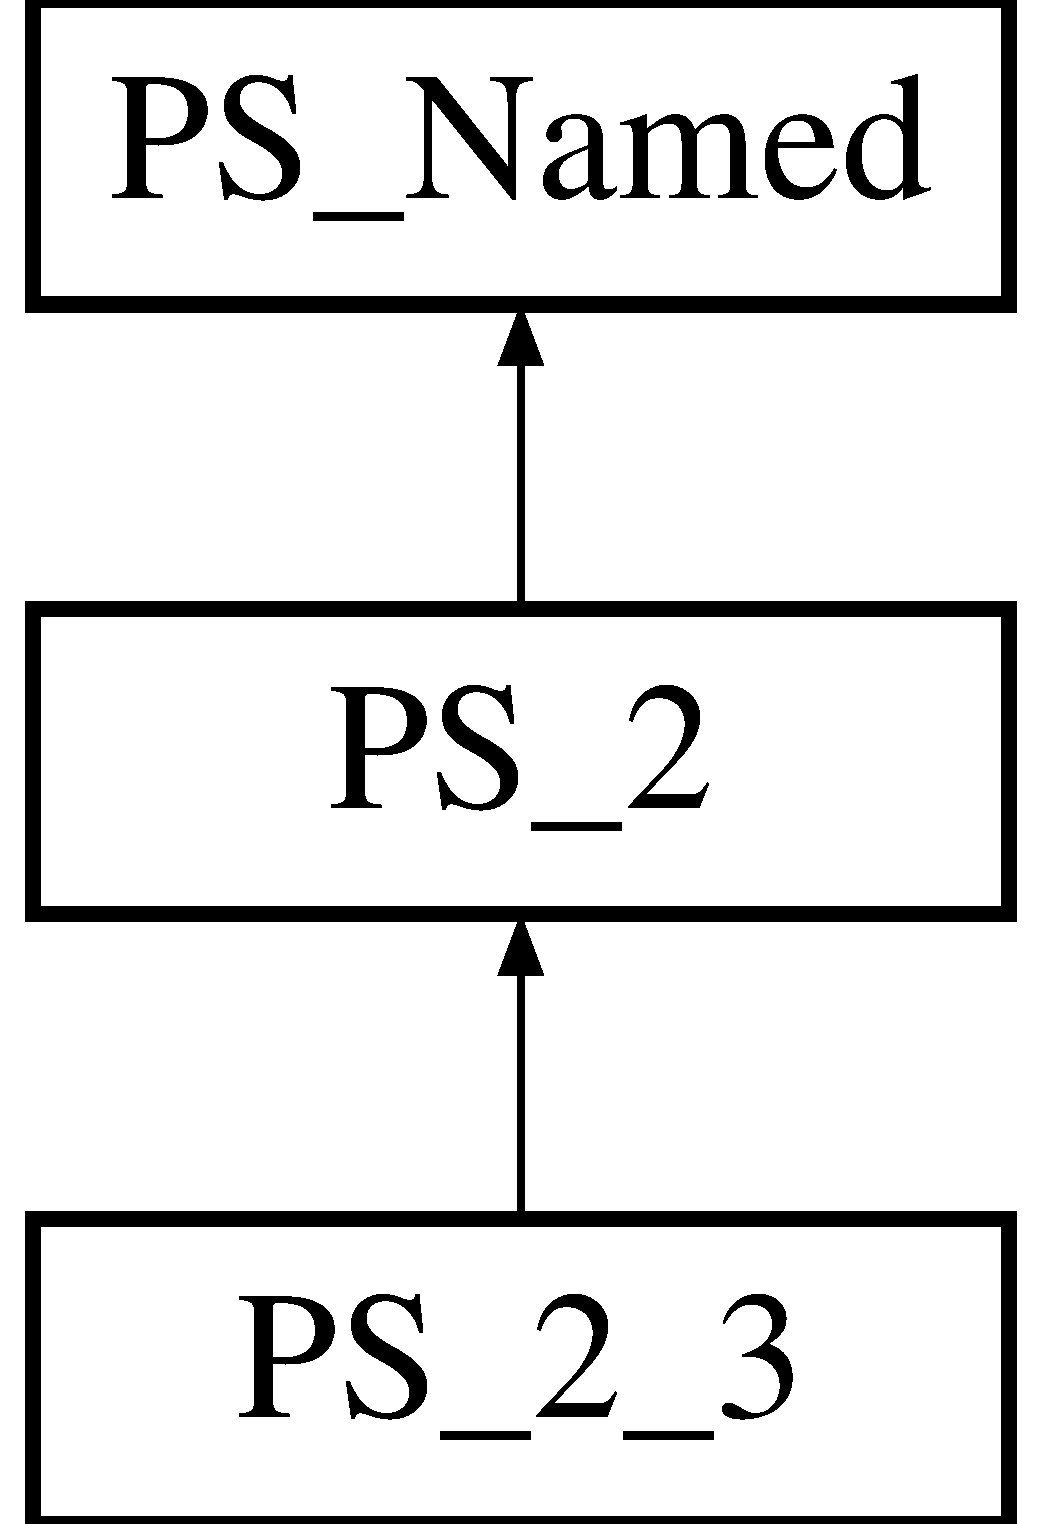
\includegraphics[height=2.000000cm]{classPS__2__3}
\end{center}
\end{figure}
\subsection*{Public Member Functions}
\begin{DoxyCompactItemize}
\item 
\hypertarget{classPS__2__3_ab8f2664ecfc751cc67758877b1faaf1a}{{\bfseries P\-S\-\_\-2\-\_\-3} (double const \&m1sq, double const \&m2sq, double const \&m3sq, const std\-::string \&nm=\char`\"{}2-\/$>$3\char`\"{})}\label{classPS__2__3_ab8f2664ecfc751cc67758877b1faaf1a}

\item 
\hypertarget{classPS__2__3_a70c48a6882d721f7bbd4303fc435f0ef}{{\bfseries P\-S\-\_\-2\-\_\-3} (const std\-::string \&nm=\char`\"{}2-\/$>$3\char`\"{})}\label{classPS__2__3_a70c48a6882d721f7bbd4303fc435f0ef}

\item 
\hypertarget{classPS__2__3_ad94c48b0f0f0d85a9fe2eda8ab86ed4c}{\hyperlink{classFV}{F\-V} const \& {\bfseries get\-\_\-k} (int i) const }\label{classPS__2__3_ad94c48b0f0f0d85a9fe2eda8ab86ed4c}

\item 
\hypertarget{classPS__2__3_a60f08c495bc4adb2c7cd172ffb5a5ee8}{\hyperlink{classPS__2}{P\-S\-\_\-2} $\ast$ {\bfseries get\-\_\-child} (int i) const }\label{classPS__2__3_a60f08c495bc4adb2c7cd172ffb5a5ee8}

\item 
\hypertarget{classPS__2__3_a4d60a9ea4e6348616b9f5359b151dac7}{double const \& {\bfseries get\-\_\-msq} (int i) const }\label{classPS__2__3_a4d60a9ea4e6348616b9f5359b151dac7}

\item 
\hypertarget{classPS__2__3_a25fc55beb243e18d8edfabdae7aa1d47}{void {\bfseries set\-\_\-msq} (double const \&m1sq, double const \&m2sq, double const \&m3sq)}\label{classPS__2__3_a25fc55beb243e18d8edfabdae7aa1d47}

\item 
\hypertarget{classPS__2__3_a859deb3d64ac6964a74a6d395d665b03}{double const \& {\bfseries get\-\_\-beta} (int i) const }\label{classPS__2__3_a859deb3d64ac6964a74a6d395d665b03}

\item 
\hypertarget{classPS__2__3_ab8b97616752d6c90ae43b3e5433dfb9c}{double const \& {\bfseries get\-\_\-y\-\_\-cm} () const }\label{classPS__2__3_ab8b97616752d6c90ae43b3e5433dfb9c}

\item 
\hypertarget{classPS__2__3_a064b972db40cb6ac0bb77232dbc31a84}{double const \& {\bfseries get\-\_\-\-M12} () const }\label{classPS__2__3_a064b972db40cb6ac0bb77232dbc31a84}

\item 
\hypertarget{classPS__2__3_a3457627140be3cc125973b9349543a54}{double const \& {\bfseries get\-\_\-y\-\_\-12} () const }\label{classPS__2__3_a3457627140be3cc125973b9349543a54}

\item 
\hypertarget{classPS__2__3_a1473a8cfc594bdc90d88304c41ab680b}{double const \& {\bfseries get\-\_\-phi\-\_\-12} () const }\label{classPS__2__3_a1473a8cfc594bdc90d88304c41ab680b}

\item 
\hypertarget{classPS__2__3_a202ec7b64ebba9be65a98d981df496d3}{\hyperlink{classFV}{F\-V} \& {\bfseries k1} ()}\label{classPS__2__3_a202ec7b64ebba9be65a98d981df496d3}

\item 
\hypertarget{classPS__2__3_a812a24d352e8c6550657abdb49c24b58}{\hyperlink{classFV}{F\-V} \& {\bfseries k2} ()}\label{classPS__2__3_a812a24d352e8c6550657abdb49c24b58}

\item 
\hypertarget{classPS__2__3_a3a779e7320a2d22b232c1cbc77b18a07}{\hyperlink{classFV}{F\-V} \& {\bfseries k3} ()}\label{classPS__2__3_a3a779e7320a2d22b232c1cbc77b18a07}

\item 
\hypertarget{classPS__2__3_a412b287c8eff0a075c6c3996b811d0c9}{\hyperlink{classFV}{F\-V} \& {\bfseries p3} ()}\label{classPS__2__3_a412b287c8eff0a075c6c3996b811d0c9}

\item 
\hypertarget{classPS__2__3_a3a74b4311b2d21c351fa7cb5beddd6b7}{\hyperlink{classFV}{F\-V} \& {\bfseries s1} ()}\label{classPS__2__3_a3a74b4311b2d21c351fa7cb5beddd6b7}

\item 
\hypertarget{classPS__2__3_a76f07efbe991b939e4afb36fe7237642}{\hyperlink{classFV}{F\-V} \& {\bfseries s2} ()}\label{classPS__2__3_a76f07efbe991b939e4afb36fe7237642}

\item 
\hypertarget{classPS__2__3_ae37a4d3ecc54651115791066f99ce803}{\hyperlink{classFV}{F\-V} \& {\bfseries s1\-\_\-r} ()}\label{classPS__2__3_ae37a4d3ecc54651115791066f99ce803}

\item 
\hypertarget{classPS__2__3_af17dff958c76a8b1873f50acd5dbc446}{\hyperlink{classFV}{F\-V} \& {\bfseries s2\-\_\-r} ()}\label{classPS__2__3_af17dff958c76a8b1873f50acd5dbc446}

\item 
\hypertarget{classPS__2__3_a512b056d5b068136ef632216f520ea53}{\hyperlink{classFV}{F\-V} const \& {\bfseries k1} () const }\label{classPS__2__3_a512b056d5b068136ef632216f520ea53}

\item 
\hypertarget{classPS__2__3_a1135303ac75b75469ceee3de6f1d03de}{\hyperlink{classFV}{F\-V} const \& {\bfseries k2} () const }\label{classPS__2__3_a1135303ac75b75469ceee3de6f1d03de}

\item 
\hypertarget{classPS__2__3_a7fab5e0b464b5bd373cfef36df34c8dd}{\hyperlink{classFV}{F\-V} const \& {\bfseries k3} () const }\label{classPS__2__3_a7fab5e0b464b5bd373cfef36df34c8dd}

\item 
\hypertarget{classPS__2__3_a4264525b624f20abba9726190a9bdaec}{\hyperlink{classFV}{F\-V} const \& {\bfseries p3} () const }\label{classPS__2__3_a4264525b624f20abba9726190a9bdaec}

\item 
\hypertarget{classPS__2__3_a8df409a98b15a028d61fd3066773892b}{\hyperlink{classFV}{F\-V} const \& {\bfseries s1} () const }\label{classPS__2__3_a8df409a98b15a028d61fd3066773892b}

\item 
\hypertarget{classPS__2__3_a447e218eba3647afcf3d24dfef90025f}{\hyperlink{classFV}{F\-V} const \& {\bfseries s2} () const }\label{classPS__2__3_a447e218eba3647afcf3d24dfef90025f}

\item 
\hypertarget{classPS__2__3_a4d40c196598e574109dd37179870363a}{\hyperlink{classFV}{F\-V} const \& {\bfseries s1\-\_\-r} () const }\label{classPS__2__3_a4d40c196598e574109dd37179870363a}

\item 
\hypertarget{classPS__2__3_ab5228f4101a880ebc59802364d347a76}{\hyperlink{classFV}{F\-V} const \& {\bfseries s2\-\_\-r} () const }\label{classPS__2__3_ab5228f4101a880ebc59802364d347a76}

\item 
\hypertarget{classPS__2__3_ad6c103ccf419ec6f416c54866d305fd0}{int {\bfseries boost\-\_\-to\-\_\-parent} ()}\label{classPS__2__3_ad6c103ccf419ec6f416c54866d305fd0}

\item 
\hypertarget{classPS__2__3_a278af8edd62fe80330a5dc5f2d385bf5}{int {\bfseries set} (double const \&rs, double const \&y\-\_\-cm, double const \&phi\-\_\-cm, double const \&M12, double const \&y\-\_\-12, double const \&phi\-\_\-12)}\label{classPS__2__3_a278af8edd62fe80330a5dc5f2d385bf5}

\item 
\hypertarget{classPS__2__3_a2da075a0d45b58fd9b4b50f6185a7368}{int {\bfseries set\-\_\-child} (int i, \hyperlink{classPS__2}{P\-S\-\_\-2} $\ast$child)}\label{classPS__2__3_a2da075a0d45b58fd9b4b50f6185a7368}

\item 
\hypertarget{classPS__2__3_ab7105d8734ec97b22c0104bd451d619b}{int {\bfseries whattype} () const }\label{classPS__2__3_ab7105d8734ec97b22c0104bd451d619b}

\item 
\hypertarget{classPS__2__3_a98b7559fbc72002c2dd6dadb1db9be0b}{void {\bfseries print} () const }\label{classPS__2__3_a98b7559fbc72002c2dd6dadb1db9be0b}

\item 
\hypertarget{classPS__2__3_a13e50836a67fad996eb544614f569a60}{void {\bfseries Fill\-Distributions} (std\-::vector$<$ \hyperlink{classHistArray}{Hist\-Array} $\ast$ $>$ \&dist, int id, double const \&wgt) const }\label{classPS__2__3_a13e50836a67fad996eb544614f569a60}

\end{DoxyCompactItemize}
\subsection*{Additional Inherited Members}


\subsection{Detailed Description}
Phase space for 2-\/$>$3 scattering. 

The documentation for this class was generated from the following files\-:\begin{DoxyCompactItemize}
\item 
inc/\hyperlink{PhaseSpace_8h}{Phase\-Space.\-h}\item 
src/Phase\-Space.\-cpp\end{DoxyCompactItemize}

\hypertarget{classPS__Named}{}\section{P\+S\+\_\+\+Named Class Reference}
\label{classPS__Named}\index{P\+S\+\_\+\+Named@{P\+S\+\_\+\+Named}}


Named base class for phase space.  




{\ttfamily \#include $<$Phase\+Space.\+h$>$}

Inheritance diagram for P\+S\+\_\+\+Named\+:\begin{figure}[H]
\begin{center}
\leavevmode
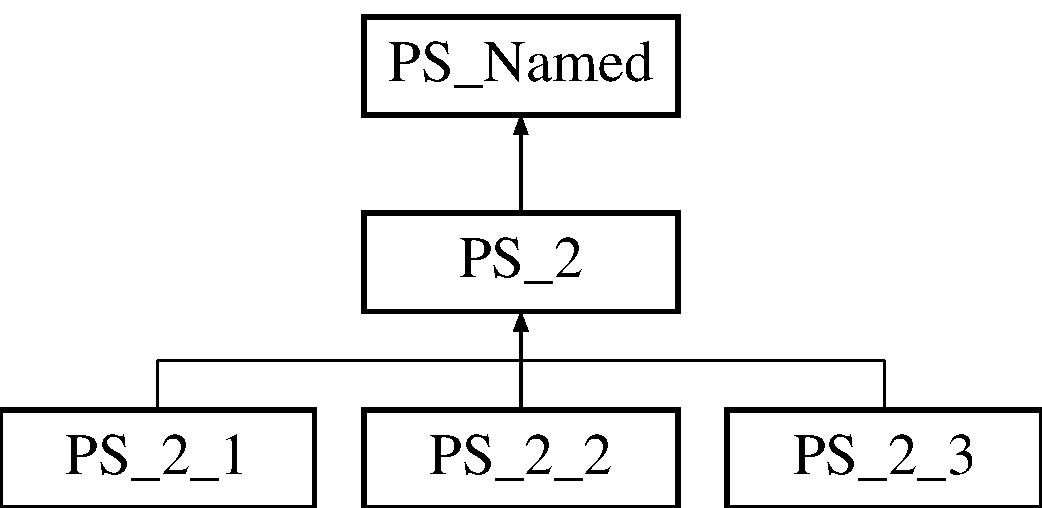
\includegraphics[height=3.000000cm]{classPS__Named}
\end{center}
\end{figure}
\subsection*{Public Member Functions}
\begin{DoxyCompactItemize}
\item 
\hypertarget{classPS__Named_ae9995f08b542e78ca1a9dc96805ebfdf}{}{\bfseries P\+S\+\_\+\+Named} (std\+::string const \&nm)\label{classPS__Named_ae9995f08b542e78ca1a9dc96805ebfdf}

\item 
\hypertarget{classPS__Named_a49250b5b43dce6fc026241d023d0e155}{}\hyperlink{classPS__Named}{P\+S\+\_\+\+Named} const \& {\bfseries operator=} (\hyperlink{classPS__Named}{P\+S\+\_\+\+Named} const \&rhs)\label{classPS__Named_a49250b5b43dce6fc026241d023d0e155}

\item 
\hypertarget{classPS__Named_ae072e1468a73ca31410d4cce3be6a6e9}{}void {\bfseries set\+\_\+name} (std\+::string const \&name)\label{classPS__Named_ae072e1468a73ca31410d4cce3be6a6e9}

\item 
\hypertarget{classPS__Named_a5b6f04214d47c462f7bc65c4ed5e867f}{}std\+::string {\bfseries get\+\_\+name} ()\label{classPS__Named_a5b6f04214d47c462f7bc65c4ed5e867f}

\end{DoxyCompactItemize}
\subsection*{Protected Attributes}
\begin{DoxyCompactItemize}
\item 
\hypertarget{classPS__Named_a4c24a47ba31313b51c2eed75fa441a4a}{}std\+::string \hyperlink{classPS__Named_a4c24a47ba31313b51c2eed75fa441a4a}{d\+\_\+name}\label{classPS__Named_a4c24a47ba31313b51c2eed75fa441a4a}

\begin{DoxyCompactList}\small\item\em name of the P\+S instance, useful to locate errors \end{DoxyCompactList}\end{DoxyCompactItemize}


\subsection{Detailed Description}
Named base class for phase space. 

With this one can use the \textquotesingle{}=\textquotesingle{} operator on all derived phase space classes whereby each instance can keep its individual name. 

Definition at line 38 of file Phase\+Space.\+h.



The documentation for this class was generated from the following file\+:\begin{DoxyCompactItemize}
\item 
inc/\hyperlink{PhaseSpace_8h}{Phase\+Space.\+h}\end{DoxyCompactItemize}

\hypertarget{classteebuf}{\section{teebuf Class Reference}
\label{classteebuf}\index{teebuf@{teebuf}}
}
Inheritance diagram for teebuf\-:\begin{figure}[H]
\begin{center}
\leavevmode
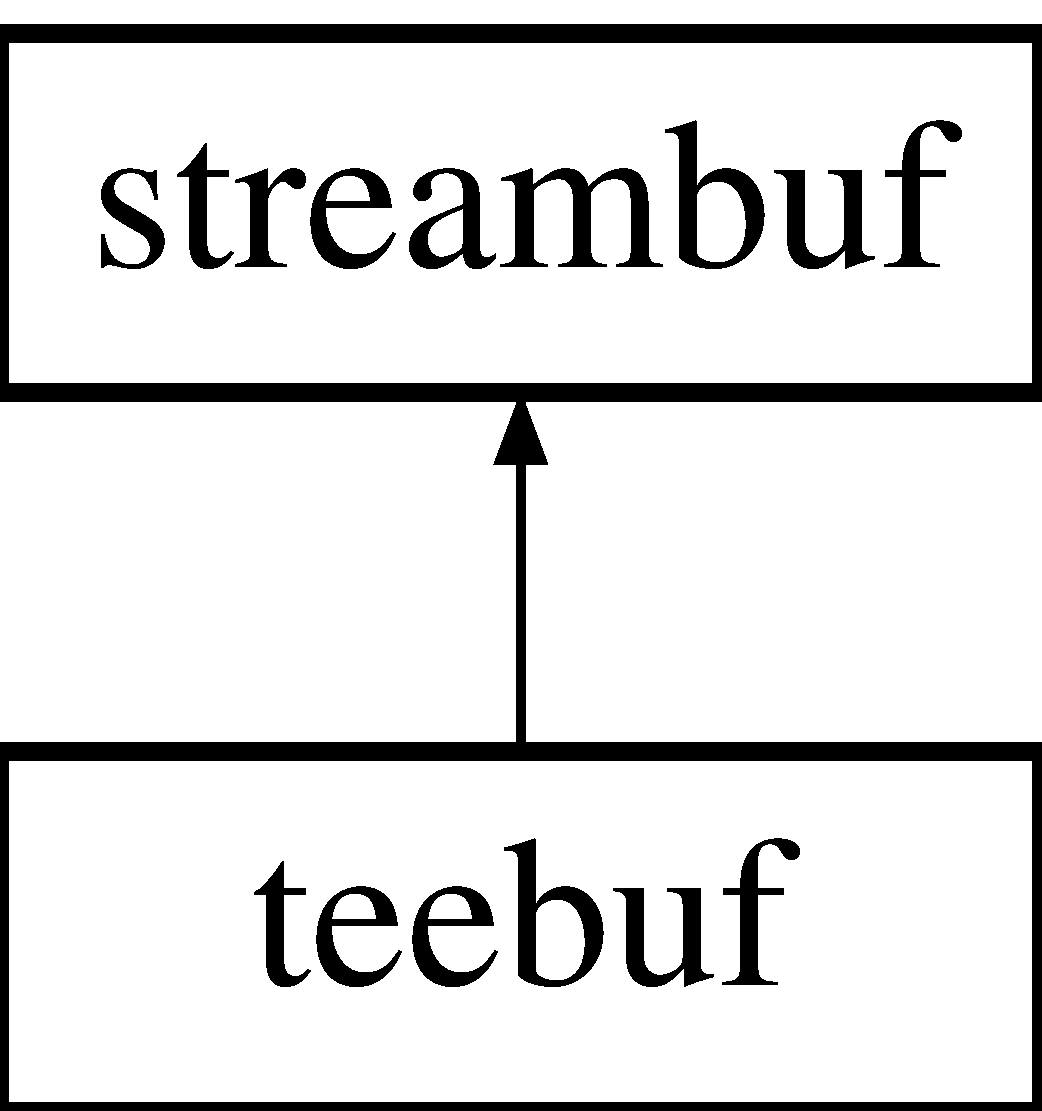
\includegraphics[height=2.000000cm]{classteebuf}
\end{center}
\end{figure}
\subsection*{Public Member Functions}
\begin{DoxyCompactItemize}
\item 
\hypertarget{classteebuf_a874f4618a07d33370216658636c23558}{\hyperlink{classteebuf_a874f4618a07d33370216658636c23558}{teebuf} (std\-::streambuf $\ast$sb1, std\-::streambuf $\ast$sb2)}\label{classteebuf_a874f4618a07d33370216658636c23558}

\begin{DoxyCompactList}\small\item\em Construct a streambuf which tees output to both input streambufs. \end{DoxyCompactList}\end{DoxyCompactItemize}


\subsection{Detailed Description}


Definition at line 92 of file Global.\-h.



The documentation for this class was generated from the following file\-:\begin{DoxyCompactItemize}
\item 
inc/\hyperlink{Global_8h}{Global.\-h}\end{DoxyCompactItemize}

\hypertarget{classteestream}{\section{teestream Class Reference}
\label{classteestream}\index{teestream@{teestream}}
}
Inheritance diagram for teestream\-:\begin{figure}[H]
\begin{center}
\leavevmode
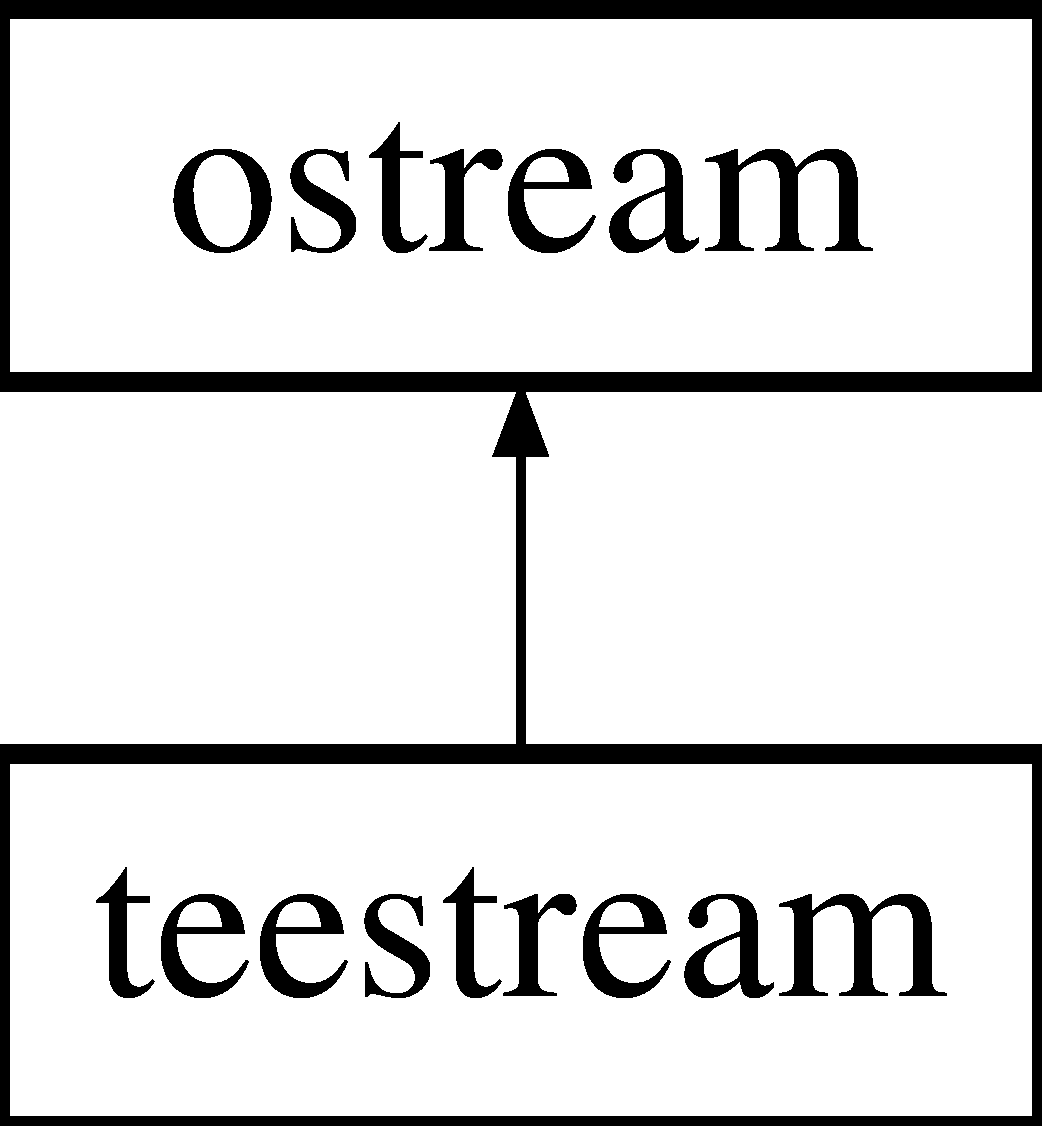
\includegraphics[height=2.000000cm]{classteestream}
\end{center}
\end{figure}
\subsection*{Public Member Functions}
\begin{DoxyCompactItemize}
\item 
\hypertarget{classteestream_aa7289fc026f510120ce669da5ad6b92e}{{\bfseries teestream} (std\-::ostream \&o1, std\-::ostream \&o2)}\label{classteestream_aa7289fc026f510120ce669da5ad6b92e}

\end{DoxyCompactItemize}


The documentation for this class was generated from the following file\-:\begin{DoxyCompactItemize}
\item 
inc/Global.\-h\end{DoxyCompactItemize}

\hypertarget{classvegas__par}{\section{vegas\-\_\-par Class Reference}
\label{classvegas__par}\index{vegas\-\_\-par@{vegas\-\_\-par}}
}


{\ttfamily \#include $<$Integrator.\-h$>$}

\subsection*{Public Member Functions}
\begin{DoxyCompactItemize}
\item 
\hypertarget{classvegas__par_a730b059d3c70a835152ca7b012e6c267}{void {\bfseries Print} (std\-::ostream \&ost=std\-::cout)}\label{classvegas__par_a730b059d3c70a835152ca7b012e6c267}

\end{DoxyCompactItemize}
\subsection*{Public Attributes}
\begin{DoxyCompactItemize}
\item 
\hypertarget{classvegas__par_a5472d94e7f8028dd706014db71351cb3}{int {\bfseries verbose}}\label{classvegas__par_a5472d94e7f8028dd706014db71351cb3}

\item 
\hypertarget{classvegas__par_a3b6da53c04f019cbdf1af4ad1863d06d}{int {\bfseries calls}}\label{classvegas__par_a3b6da53c04f019cbdf1af4ad1863d06d}

\item 
\hypertarget{classvegas__par_ace66e9b903313d9e11716174c17ee6e7}{int {\bfseries iterations}}\label{classvegas__par_ace66e9b903313d9e11716174c17ee6e7}

\item 
\hypertarget{classvegas__par_a80b974e1bf642b29945dfd3438efbc34}{int {\bfseries max\-\_\-runs}}\label{classvegas__par_a80b974e1bf642b29945dfd3438efbc34}

\item 
\hypertarget{classvegas__par_a2810d1e8ab5310e718ebaeca2a76fe28}{int {\bfseries num\-\_\-runs}}\label{classvegas__par_a2810d1e8ab5310e718ebaeca2a76fe28}

\item 
\hypertarget{classvegas__par_acc595720db25ce8eab7226cdec4c6420}{double {\bfseries chisq\-\_\-limit}}\label{classvegas__par_acc595720db25ce8eab7226cdec4c6420}

\item 
\hypertarget{classvegas__par_a3b779550ebda38d7faae46b47170413f}{double {\bfseries chisq}}\label{classvegas__par_a3b779550ebda38d7faae46b47170413f}

\item 
\hypertarget{classvegas__par_a25e768ececdfec2ba412474b515ee574}{bool {\bfseries do\-\_\-warmup}}\label{classvegas__par_a25e768ececdfec2ba412474b515ee574}

\item 
\hypertarget{classvegas__par_aeeaf46c74fb3b394bb7f30f6f74ff3e8}{bool {\bfseries grid\-\_\-fixed}}\label{classvegas__par_aeeaf46c74fb3b394bb7f30f6f74ff3e8}

\item 
\hypertarget{classvegas__par_aa4410a8632fb15ee6c5592dabdafd7b8}{double {\bfseries result}}\label{classvegas__par_aa4410a8632fb15ee6c5592dabdafd7b8}

\item 
\hypertarget{classvegas__par_ac0f80dfd49fa917435c9c4e2a480198e}{double {\bfseries error}}\label{classvegas__par_ac0f80dfd49fa917435c9c4e2a480198e}

\end{DoxyCompactItemize}


\subsection{Detailed Description}
This class contains the parameters to control the G\-S\-L V\-E\-G\-A\-S algorithm. 

Definition at line 35 of file Integrator.\-h.



The documentation for this class was generated from the following files\-:\begin{DoxyCompactItemize}
\item 
inc/\hyperlink{Integrator_8h}{Integrator.\-h}\item 
src/Integrator.\-cpp\end{DoxyCompactItemize}

\chapter{File Documentation}
\hypertarget{FileBrowser_8h}{}\section{inc/\+File\+Browser.h File Reference}
\label{FileBrowser_8h}\index{inc/\+File\+Browser.\+h@{inc/\+File\+Browser.\+h}}


Simple, text-\/based file browser.  


{\ttfamily \#include $<$iostream$>$}\\*
{\ttfamily \#include $<$iomanip$>$}\\*
{\ttfamily \#include $<$sstream$>$}\\*
{\ttfamily \#include \char`\"{}boost/filesystem.\+hpp\char`\"{}}\\*
\subsection*{Classes}
\begin{DoxyCompactItemize}
\item 
class \hyperlink{classFileBrowser}{File\+Browser}
\begin{DoxyCompactList}\small\item\em Simple, text-\/based file browser class. \end{DoxyCompactList}\end{DoxyCompactItemize}


\subsection{Detailed Description}
Simple, text-\/based file browser. 


\hypertarget{Flags_8h}{}\section{inc/\+Flags.h File Reference}
\label{Flags_8h}\index{inc/\+Flags.\+h@{inc/\+Flags.\+h}}


Flags to control the evaluation of sub amplitudes.  


{\ttfamily \#include $<$boost/utility.\+hpp$>$}\\*
\subsection*{Macros}
\begin{DoxyCompactItemize}
\item 
\#define \hyperlink{Flags_8h_a82849e83012283f0702b28b15bfe7e14}{I\+\_\+\+F\+L\+A\+G\+S\+\_\+\+A\+L\+L}~B\+O\+O\+S\+T\+\_\+\+B\+I\+N\+A\+R\+Y(1 111 111 1)
\item 
\hypertarget{Flags_8h_ac2348ab835e5e5e8216710b03f3e580e}{}\#define \hyperlink{Flags_8h_ac2348ab835e5e5e8216710b03f3e580e}{I\+\_\+\+F\+L\+A\+G\+S\+\_\+\+B\+\_\+\+Q\+C\+D}~B\+O\+O\+S\+T\+\_\+\+B\+I\+N\+A\+R\+Y(0 000 000 1)\label{Flags_8h_ac2348ab835e5e5e8216710b03f3e580e}

\begin{DoxyCompactList}\small\item\em Integrate L\+O Q\+C\+D contribution. \end{DoxyCompactList}\item 
\hypertarget{Flags_8h_ae65cb02713d911b61b74499b168eab71}{}\#define \hyperlink{Flags_8h_ae65cb02713d911b61b74499b168eab71}{I\+\_\+\+F\+L\+A\+G\+S\+\_\+\+B\+\_\+\+P\+H\+I}~B\+O\+O\+S\+T\+\_\+\+B\+I\+N\+A\+R\+Y(0 000 001 0)\label{Flags_8h_ae65cb02713d911b61b74499b168eab71}

\begin{DoxyCompactList}\small\item\em Integrate L\+O (P\+H\+Ix\+P\+H\+I+\+P\+H\+Ix\+Q\+C\+D) contribution. \end{DoxyCompactList}\item 
\hypertarget{Flags_8h_ad129cd07ca6cfb6cd2831c2ce331b688}{}\#define \hyperlink{Flags_8h_ad129cd07ca6cfb6cd2831c2ce331b688}{I\+\_\+\+F\+L\+A\+G\+S\+\_\+\+B}~B\+O\+O\+S\+T\+\_\+\+B\+I\+N\+A\+R\+Y(0 000 001 1)\label{Flags_8h_ad129cd07ca6cfb6cd2831c2ce331b688}

\begin{DoxyCompactList}\small\item\em Integrate both L\+O contributions. \end{DoxyCompactList}\item 
\hypertarget{Flags_8h_a6ad01071e5d5fe879f5d08d105788ded}{}\#define \hyperlink{Flags_8h_a6ad01071e5d5fe879f5d08d105788ded}{I\+\_\+\+F\+L\+A\+G\+S\+\_\+\+V}~B\+O\+O\+S\+T\+\_\+\+B\+I\+N\+A\+R\+Y(0 000 010 0)\label{Flags_8h_a6ad01071e5d5fe879f5d08d105788ded}

\begin{DoxyCompactList}\small\item\em Integrate virtual corrections. \end{DoxyCompactList}\item 
\hypertarget{Flags_8h_a9f9f2a586a70083f7ad3d2b6395cd44e}{}\#define \hyperlink{Flags_8h_a9f9f2a586a70083f7ad3d2b6395cd44e}{I\+\_\+\+F\+L\+A\+G\+S\+\_\+\+D}~B\+O\+O\+S\+T\+\_\+\+B\+I\+N\+A\+R\+Y(0 000 100 0)\label{Flags_8h_a9f9f2a586a70083f7ad3d2b6395cd44e}

\begin{DoxyCompactList}\small\item\em Integrate integrated dipoles. \end{DoxyCompactList}\item 
\hypertarget{Flags_8h_a89fe42849457cd534db2e985349a501c}{}\#define \hyperlink{Flags_8h_a89fe42849457cd534db2e985349a501c}{I\+\_\+\+F\+L\+A\+G\+S\+\_\+\+R\+\_\+\+G\+G}~B\+O\+O\+S\+T\+\_\+\+B\+I\+N\+A\+R\+Y(0 001 000 0)\label{Flags_8h_a89fe42849457cd534db2e985349a501c}

\begin{DoxyCompactList}\small\item\em Integrate real corrections with gg initial state. \end{DoxyCompactList}\item 
\hypertarget{Flags_8h_ad9c441b5eebfd3f69bb9a525b51b04cf}{}\#define \hyperlink{Flags_8h_ad9c441b5eebfd3f69bb9a525b51b04cf}{I\+\_\+\+F\+L\+A\+G\+S\+\_\+\+R\+\_\+\+Q\+Q}~B\+O\+O\+S\+T\+\_\+\+B\+I\+N\+A\+R\+Y(0 010 000 0)\label{Flags_8h_ad9c441b5eebfd3f69bb9a525b51b04cf}

\begin{DoxyCompactList}\small\item\em Integrate real corrections with qq initial state. \end{DoxyCompactList}\item 
\hypertarget{Flags_8h_ad6ee44de025531d26d782d1bdee5c647}{}\#define \hyperlink{Flags_8h_ad6ee44de025531d26d782d1bdee5c647}{I\+\_\+\+F\+L\+A\+G\+S\+\_\+\+R\+\_\+\+Q\+G}~B\+O\+O\+S\+T\+\_\+\+B\+I\+N\+A\+R\+Y(0 100 000 0)\label{Flags_8h_ad6ee44de025531d26d782d1bdee5c647}

\begin{DoxyCompactList}\small\item\em Integrate real corrections with qg initial state. \end{DoxyCompactList}\item 
\hypertarget{Flags_8h_a6e54d9c2d49b350bc5342b08a306c9ed}{}\#define \hyperlink{Flags_8h_a6e54d9c2d49b350bc5342b08a306c9ed}{I\+\_\+\+F\+L\+A\+G\+S\+\_\+\+P\+L\+O\+T}~B\+O\+O\+S\+T\+\_\+\+B\+I\+N\+A\+R\+Y(1 000 000 0)\label{Flags_8h_a6e54d9c2d49b350bc5342b08a306c9ed}

\begin{DoxyCompactList}\small\item\em Integrate real corrections with gg initial state. \end{DoxyCompactList}\item 
\hypertarget{Flags_8h_ad17b2e7317b27594cfcefdcaae70c870}{}\#define {\bfseries S\+E\+T\+\_\+\+F\+L\+A\+G}(F\+L\+A\+G,  F)~F $\vert$=  F\+L\+A\+G\label{Flags_8h_ad17b2e7317b27594cfcefdcaae70c870}

\item 
\hypertarget{Flags_8h_a117d812510939322fc2f83ea37bd8670}{}\#define {\bfseries U\+S\+E\+T\+\_\+\+F\+L\+A\+G}(F\+L\+A\+G,  F)~F \&= $\sim$F\+L\+A\+G\label{Flags_8h_a117d812510939322fc2f83ea37bd8670}

\item 
\hypertarget{Flags_8h_ac2ce8f00f5a3818c2e83429207e9611f}{}\#define \hyperlink{Flags_8h_ac2ce8f00f5a3818c2e83429207e9611f}{F\+\_\+\+E\+V\+A\+L\+\_\+\+A\+L\+L}~B\+O\+O\+S\+T\+\_\+\+B\+I\+N\+A\+R\+Y\+\_\+\+L\+U(111 111 111 111 111 111 111 1)\label{Flags_8h_ac2ce8f00f5a3818c2e83429207e9611f}

\begin{DoxyCompactList}\small\item\em Evaluate all sub-\/amplitudes. \end{DoxyCompactList}\item 
\hypertarget{Flags_8h_a278ec3a660bd62f835cf1c170bd9ea5a}{}\#define \hyperlink{Flags_8h_a278ec3a660bd62f835cf1c170bd9ea5a}{F\+\_\+\+E\+V\+A\+L\+\_\+\+B\+\_\+\+A\+L\+L}~B\+O\+O\+S\+T\+\_\+\+B\+I\+N\+A\+R\+Y\+\_\+\+L\+U(000 000 000 000 000 000 111 0)\label{Flags_8h_a278ec3a660bd62f835cf1c170bd9ea5a}

\begin{DoxyCompactList}\small\item\em Evaluate all L\+O amplitudes. \end{DoxyCompactList}\item 
\hypertarget{Flags_8h_a382b0eae8408260d329197173ca3d5a3}{}\#define \hyperlink{Flags_8h_a382b0eae8408260d329197173ca3d5a3}{F\+\_\+\+E\+V\+A\+L\+\_\+\+B\+\_\+\+P\+H\+Ix\+P\+H\+I}~B\+O\+O\+S\+T\+\_\+\+B\+I\+N\+A\+R\+Y\+\_\+\+L\+U(000 000 000 000 000 000 001 0)\label{Flags_8h_a382b0eae8408260d329197173ca3d5a3}

\begin{DoxyCompactList}\small\item\em Evaluate L\+O P\+H\+Ix\+P\+H\+I amplitudes. \end{DoxyCompactList}\item 
\hypertarget{Flags_8h_abe4da41ec421ae0731d3ec791d150d9a}{}\#define \hyperlink{Flags_8h_abe4da41ec421ae0731d3ec791d150d9a}{F\+\_\+\+E\+V\+A\+L\+\_\+\+B\+\_\+\+P\+H\+Ix\+Q\+C\+D}~B\+O\+O\+S\+T\+\_\+\+B\+I\+N\+A\+R\+Y\+\_\+\+L\+U(000 000 000 000 000 000 010 0)\label{Flags_8h_abe4da41ec421ae0731d3ec791d150d9a}

\begin{DoxyCompactList}\small\item\em Evaluate L\+O P\+H\+Ix\+Q\+C\+D amplitudes. \end{DoxyCompactList}\item 
\hypertarget{Flags_8h_adb684c9a5a7b99ed5e54ee0847867fd1}{}\#define \hyperlink{Flags_8h_adb684c9a5a7b99ed5e54ee0847867fd1}{F\+\_\+\+E\+V\+A\+L\+\_\+\+B\+\_\+\+Q\+C\+Dx\+Q\+C\+D}~B\+O\+O\+S\+T\+\_\+\+B\+I\+N\+A\+R\+Y\+\_\+\+L\+U(000 000 000 000 000 000 100 0)\label{Flags_8h_adb684c9a5a7b99ed5e54ee0847867fd1}

\begin{DoxyCompactList}\small\item\em Evaluate L\+O Q\+C\+D amplitudes. \end{DoxyCompactList}\item 
\hypertarget{Flags_8h_afaae1aaf2d8a805a45b1498b251934e5}{}\#define \hyperlink{Flags_8h_afaae1aaf2d8a805a45b1498b251934e5}{F\+\_\+\+E\+V\+A\+L\+\_\+\+V\+\_\+\+A\+L\+L}~B\+O\+O\+S\+T\+\_\+\+B\+I\+N\+A\+R\+Y\+\_\+\+L\+U(000 000 111 111 111 111 000 0)\label{Flags_8h_afaae1aaf2d8a805a45b1498b251934e5}

\begin{DoxyCompactList}\small\item\em Evaluate all virtual amplitudes. \end{DoxyCompactList}\item 
\hypertarget{Flags_8h_a034edf1bfbab5a9f18c271dc2e265180}{}\#define \hyperlink{Flags_8h_a034edf1bfbab5a9f18c271dc2e265180}{F\+\_\+\+E\+V\+A\+L\+\_\+\+V\+\_\+\+P\+H\+I0x\+Q\+C\+D1}~B\+O\+O\+S\+T\+\_\+\+B\+I\+N\+A\+R\+Y\+\_\+\+L\+U(000 000 001 111 111 111 000 0)\label{Flags_8h_a034edf1bfbab5a9f18c271dc2e265180}

\begin{DoxyCompactList}\small\item\em Evaluate all virtual P\+H\+I0x\+Q\+C\+D1 amplitudes. \end{DoxyCompactList}\item 
\hypertarget{Flags_8h_ab07c58a16fd549bd49e9492865952abf}{}\#define \hyperlink{Flags_8h_ab07c58a16fd549bd49e9492865952abf}{F\+\_\+\+E\+V\+A\+L\+\_\+\+V\+\_\+\+S\+E}~B\+O\+O\+S\+T\+\_\+\+B\+I\+N\+A\+R\+Y\+\_\+\+L\+U(000 000 000 000 000 001 000 0)\label{Flags_8h_ab07c58a16fd549bd49e9492865952abf}

\begin{DoxyCompactList}\small\item\em Evaluate virtual P\+H\+I0x\+Q\+C\+D1 self-\/energy amplitude. \end{DoxyCompactList}\item 
\hypertarget{Flags_8h_a884809cd7071fd93c8b13fd49b721d69}{}\#define \hyperlink{Flags_8h_a884809cd7071fd93c8b13fd49b721d69}{F\+\_\+\+E\+V\+A\+L\+\_\+\+V\+\_\+\+C\+T\+S\+E}~B\+O\+O\+S\+T\+\_\+\+B\+I\+N\+A\+R\+Y\+\_\+\+L\+U(000 000 000 000 000 010 000 0)\label{Flags_8h_a884809cd7071fd93c8b13fd49b721d69}

\begin{DoxyCompactList}\small\item\em Evaluate virtual P\+H\+I0x\+Q\+C\+D1 self-\/energy counterterm. \end{DoxyCompactList}\item 
\hypertarget{Flags_8h_aaa1b79549ba41276e4327a5a1fe6f88c}{}\#define \hyperlink{Flags_8h_aaa1b79549ba41276e4327a5a1fe6f88c}{F\+\_\+\+E\+V\+A\+L\+\_\+\+V\+\_\+4\+G}~B\+O\+O\+S\+T\+\_\+\+B\+I\+N\+A\+R\+Y\+\_\+\+L\+U(000 000 000 000 000 100 000 0)\label{Flags_8h_aaa1b79549ba41276e4327a5a1fe6f88c}

\begin{DoxyCompactList}\small\item\em Evaluate virtual P\+H\+I0x\+Q\+C\+D1 4-\/gluon amplitude. \end{DoxyCompactList}\item 
\hypertarget{Flags_8h_ad330cb2a39ce0717211f1fdc17c04e63}{}\#define \hyperlink{Flags_8h_ad330cb2a39ce0717211f1fdc17c04e63}{F\+\_\+\+E\+V\+A\+L\+\_\+\+V\+\_\+\+V1}~B\+O\+O\+S\+T\+\_\+\+B\+I\+N\+A\+R\+Y\+\_\+\+L\+U(000 000 000 000 001 000 000 0)\label{Flags_8h_ad330cb2a39ce0717211f1fdc17c04e63}

\begin{DoxyCompactList}\small\item\em Evaluate virtual P\+H\+I0x\+Q\+C\+D1 upper vertex correction. \end{DoxyCompactList}\item 
\hypertarget{Flags_8h_a3e72615bc9c26aea3b37d547dce1fcc3}{}\#define \hyperlink{Flags_8h_a3e72615bc9c26aea3b37d547dce1fcc3}{F\+\_\+\+E\+V\+A\+L\+\_\+\+V\+\_\+\+C\+T\+V1}~B\+O\+O\+S\+T\+\_\+\+B\+I\+N\+A\+R\+Y\+\_\+\+L\+U(000 000 000 000 010 000 000 0)\label{Flags_8h_a3e72615bc9c26aea3b37d547dce1fcc3}

\begin{DoxyCompactList}\small\item\em Evaluate virtual P\+H\+I0x\+Q\+C\+D1 upper vertex counterterm. \end{DoxyCompactList}\item 
\hypertarget{Flags_8h_a73b48a44db385153b3a0a237fc428c52}{}\#define \hyperlink{Flags_8h_a73b48a44db385153b3a0a237fc428c52}{F\+\_\+\+E\+V\+A\+L\+\_\+\+V\+\_\+\+V2}~B\+O\+O\+S\+T\+\_\+\+B\+I\+N\+A\+R\+Y\+\_\+\+L\+U(000 000 000 000 100 000 000 0)\label{Flags_8h_a73b48a44db385153b3a0a237fc428c52}

\begin{DoxyCompactList}\small\item\em Evaluate virtual P\+H\+I0x\+Q\+C\+D1 lower vertex correction. \end{DoxyCompactList}\item 
\hypertarget{Flags_8h_a82c1a832bec4e1fa08957c74e5c7454f}{}\#define \hyperlink{Flags_8h_a82c1a832bec4e1fa08957c74e5c7454f}{F\+\_\+\+E\+V\+A\+L\+\_\+\+V\+\_\+\+C\+T\+V2}~B\+O\+O\+S\+T\+\_\+\+B\+I\+N\+A\+R\+Y\+\_\+\+L\+U(000 000 000 001 000 000 000 0)\label{Flags_8h_a82c1a832bec4e1fa08957c74e5c7454f}

\begin{DoxyCompactList}\small\item\em Evaluate virtual P\+H\+I0x\+Q\+C\+D1 lower vertex counterterm. \end{DoxyCompactList}\item 
\hypertarget{Flags_8h_a6df9c76661db7b2d4bd31d0a20de4238}{}\#define \hyperlink{Flags_8h_a6df9c76661db7b2d4bd31d0a20de4238}{F\+\_\+\+E\+V\+A\+L\+\_\+\+V\+\_\+\+B1}~B\+O\+O\+S\+T\+\_\+\+B\+I\+N\+A\+R\+Y\+\_\+\+L\+U(000 000 000 010 000 000 000 0)\label{Flags_8h_a6df9c76661db7b2d4bd31d0a20de4238}

\begin{DoxyCompactList}\small\item\em Evaluate virtual P\+H\+I0x\+Q\+C\+D1 box 1 amplitude. \end{DoxyCompactList}\item 
\hypertarget{Flags_8h_a5577fc511922a1f9dae7d4bd4edd9546}{}\#define \hyperlink{Flags_8h_a5577fc511922a1f9dae7d4bd4edd9546}{F\+\_\+\+E\+V\+A\+L\+\_\+\+V\+\_\+\+B2}~B\+O\+O\+S\+T\+\_\+\+B\+I\+N\+A\+R\+Y\+\_\+\+L\+U(000 000 000 100 000 000 000 0)\label{Flags_8h_a5577fc511922a1f9dae7d4bd4edd9546}

\begin{DoxyCompactList}\small\item\em Evaluate virtual P\+H\+I0x\+Q\+C\+D1 box 2 amplitude. \end{DoxyCompactList}\item 
\hypertarget{Flags_8h_a0c67cdaad634470a7e06b22962fbbbe2}{}\#define \hyperlink{Flags_8h_a0c67cdaad634470a7e06b22962fbbbe2}{F\+\_\+\+E\+V\+A\+L\+\_\+\+V\+\_\+\+B3}~B\+O\+O\+S\+T\+\_\+\+B\+I\+N\+A\+R\+Y\+\_\+\+L\+U(000 000 001 000 000 000 000 0)\label{Flags_8h_a0c67cdaad634470a7e06b22962fbbbe2}

\begin{DoxyCompactList}\small\item\em Evaluate virtual P\+H\+I0x\+Q\+C\+D1 box 3 amplitude. \end{DoxyCompactList}\item 
\hypertarget{Flags_8h_af81920aa4729032241094208d081a5c5}{}\#define \hyperlink{Flags_8h_af81920aa4729032241094208d081a5c5}{F\+\_\+\+E\+V\+A\+L\+\_\+\+V\+\_\+\+P\+H\+I1x\+Q\+C\+D0}~B\+O\+O\+S\+T\+\_\+\+B\+I\+N\+A\+R\+Y\+\_\+\+L\+U(000 000 010 000 000 000 000 0)\label{Flags_8h_af81920aa4729032241094208d081a5c5}

\begin{DoxyCompactList}\small\item\em Evaluate virtual P\+H\+I1x\+Q\+C\+D0 amplitude. \end{DoxyCompactList}\item 
\hypertarget{Flags_8h_a868b0f70f5031c0d416e8ef94d729552}{}\#define \hyperlink{Flags_8h_a868b0f70f5031c0d416e8ef94d729552}{F\+\_\+\+E\+V\+A\+L\+\_\+\+V\+\_\+\+P\+H\+Ix\+P\+H\+I}~B\+O\+O\+S\+T\+\_\+\+B\+I\+N\+A\+R\+Y\+\_\+\+L\+U(000 000 100 000 000 000 000 0)\label{Flags_8h_a868b0f70f5031c0d416e8ef94d729552}

\begin{DoxyCompactList}\small\item\em Evaluate virtual P\+H\+I1x\+P\+H\+I0 amplitudes. \end{DoxyCompactList}\item 
\hypertarget{Flags_8h_a01ad4a457e642e6a7b919b50605ddf3b}{}\#define \hyperlink{Flags_8h_a01ad4a457e642e6a7b919b50605ddf3b}{F\+\_\+\+E\+V\+A\+L\+\_\+\+V\+\_\+\+N\+F}~B\+O\+O\+S\+T\+\_\+\+B\+I\+N\+A\+R\+Y\+\_\+\+L\+U(000 001 000 000 000 000 000 0)\label{Flags_8h_a01ad4a457e642e6a7b919b50605ddf3b}

\begin{DoxyCompactList}\small\item\em Evaluate non-\/factorizable virtual amplitudes. \end{DoxyCompactList}\item 
\hypertarget{Flags_8h_a54060fd0e847d88763829a606c9dc5ee}{}\#define \hyperlink{Flags_8h_a54060fd0e847d88763829a606c9dc5ee}{F\+\_\+\+E\+V\+A\+L\+\_\+\+D\+\_\+\+A\+L\+L}~B\+O\+O\+S\+T\+\_\+\+B\+I\+N\+A\+R\+Y\+\_\+\+L\+U(111 100 000 000 000 000 000 0)\label{Flags_8h_a54060fd0e847d88763829a606c9dc5ee}

\begin{DoxyCompactList}\small\item\em Evaluate all integrated dipoles. \end{DoxyCompactList}\item 
\hypertarget{Flags_8h_aaa0c5aa3516e1b94bcdb93214c2163bb}{}\#define \hyperlink{Flags_8h_aaa0c5aa3516e1b94bcdb93214c2163bb}{F\+\_\+\+E\+V\+A\+L\+\_\+\+D\+\_\+\+Q\+G\+\_\+\+C\+O\+N\+T}~B\+O\+O\+S\+T\+\_\+\+B\+I\+N\+A\+R\+Y\+\_\+\+L\+U(000 100 000 000 000 000 000 0)\label{Flags_8h_aaa0c5aa3516e1b94bcdb93214c2163bb}

\begin{DoxyCompactList}\small\item\em Evaluate continuum part of integrated dipooles corresponding to qg initial statet. \end{DoxyCompactList}\item 
\hypertarget{Flags_8h_a57d5ce95ffdb3880137329c22615e8f3}{}\#define \hyperlink{Flags_8h_a57d5ce95ffdb3880137329c22615e8f3}{F\+\_\+\+E\+V\+A\+L\+\_\+\+D\+\_\+\+G\+G\+\_\+\+A\+L\+L}~B\+O\+O\+S\+T\+\_\+\+B\+I\+N\+A\+R\+Y\+\_\+\+L\+U(111 000 000 000 000 000 000 0)\label{Flags_8h_a57d5ce95ffdb3880137329c22615e8f3}

\begin{DoxyCompactList}\small\item\em Evaluate all integrated dipooles corresponding to gg initial state. \end{DoxyCompactList}\item 
\hypertarget{Flags_8h_af6f2ccc6fd003a2c33593acca9f88bf4}{}\#define \hyperlink{Flags_8h_af6f2ccc6fd003a2c33593acca9f88bf4}{F\+\_\+\+E\+V\+A\+L\+\_\+\+D\+\_\+\+G\+G\+\_\+\+D\+E\+L\+T\+A}~B\+O\+O\+S\+T\+\_\+\+B\+I\+N\+A\+R\+Y\+\_\+\+L\+U(001 000 000 000 000 000 000 0)\label{Flags_8h_af6f2ccc6fd003a2c33593acca9f88bf4}

\begin{DoxyCompactList}\small\item\em Evaluate delta distribution terms of integrated dipooles corresponding to gg initial state. \end{DoxyCompactList}\item 
\hypertarget{Flags_8h_a53774bab74d633807e801ccac8c86c4f}{}\#define \hyperlink{Flags_8h_a53774bab74d633807e801ccac8c86c4f}{F\+\_\+\+E\+V\+A\+L\+\_\+\+D\+\_\+\+G\+G\+\_\+\+E\+N\+D}~B\+O\+O\+S\+T\+\_\+\+B\+I\+N\+A\+R\+Y\+\_\+\+L\+U(010 000 000 000 000 000 000 0)\label{Flags_8h_a53774bab74d633807e801ccac8c86c4f}

\begin{DoxyCompactList}\small\item\em Evaluate endpoint part of integrated dipooles corresponding to gg initial state. \end{DoxyCompactList}\item 
\hypertarget{Flags_8h_a8a7cfad5c9a577d6e9c306eb54ac20c7}{}\#define \hyperlink{Flags_8h_a8a7cfad5c9a577d6e9c306eb54ac20c7}{F\+\_\+\+E\+V\+A\+L\+\_\+\+D\+\_\+\+G\+G\+\_\+\+C\+O\+N\+T}~B\+O\+O\+S\+T\+\_\+\+B\+I\+N\+A\+R\+Y\+\_\+\+L\+U(100 000 000 000 000 000 000 0)\label{Flags_8h_a8a7cfad5c9a577d6e9c306eb54ac20c7}

\begin{DoxyCompactList}\small\item\em Evaluate continuum part of integrated dipooles corresponding to gg initial state. \end{DoxyCompactList}\item 
\hypertarget{Flags_8h_ade8bfe6e4856acee059cb16f8e4252d2}{}\#define {\bfseries S\+E\+T\+\_\+\+E\+V\+A\+L\+\_\+\+A\+L\+L}(F)~F $\vert$= \hyperlink{Flags_8h_ac2ce8f00f5a3818c2e83429207e9611f}{F\+\_\+\+E\+V\+A\+L\+\_\+\+A\+L\+L}\label{Flags_8h_ade8bfe6e4856acee059cb16f8e4252d2}

\item 
\hypertarget{Flags_8h_a1513090ee67b7a25bafc2663c2af672d}{}\#define {\bfseries S\+E\+T\+\_\+\+E\+V\+A\+L\+\_\+\+B\+\_\+\+A\+L\+L}(F)~F $\vert$= \hyperlink{Flags_8h_a278ec3a660bd62f835cf1c170bd9ea5a}{F\+\_\+\+E\+V\+A\+L\+\_\+\+B\+\_\+\+A\+L\+L}\label{Flags_8h_a1513090ee67b7a25bafc2663c2af672d}

\item 
\hypertarget{Flags_8h_a46534238c3f04c07d5f5305d7ee87e88}{}\#define {\bfseries S\+E\+T\+\_\+\+E\+V\+A\+L\+\_\+\+B\+\_\+\+P\+H\+Ix\+P\+H\+I}(F)~F $\vert$= \hyperlink{Flags_8h_a382b0eae8408260d329197173ca3d5a3}{F\+\_\+\+E\+V\+A\+L\+\_\+\+B\+\_\+\+P\+H\+Ix\+P\+H\+I}\label{Flags_8h_a46534238c3f04c07d5f5305d7ee87e88}

\item 
\hypertarget{Flags_8h_a22ee48fe6781aa21fa0e5462cfddddd4}{}\#define {\bfseries S\+E\+T\+\_\+\+E\+V\+A\+L\+\_\+\+B\+\_\+\+P\+H\+Ix\+Q\+C\+D}(F)~F $\vert$= \hyperlink{Flags_8h_abe4da41ec421ae0731d3ec791d150d9a}{F\+\_\+\+E\+V\+A\+L\+\_\+\+B\+\_\+\+P\+H\+Ix\+Q\+C\+D}\label{Flags_8h_a22ee48fe6781aa21fa0e5462cfddddd4}

\item 
\hypertarget{Flags_8h_af35b962c6e4675bb8fa8a72eefe1abee}{}\#define {\bfseries S\+E\+T\+\_\+\+E\+V\+A\+L\+\_\+\+B\+\_\+\+Q\+C\+Dx\+Q\+C\+D}(F)~F $\vert$= \hyperlink{Flags_8h_adb684c9a5a7b99ed5e54ee0847867fd1}{F\+\_\+\+E\+V\+A\+L\+\_\+\+B\+\_\+\+Q\+C\+Dx\+Q\+C\+D}\label{Flags_8h_af35b962c6e4675bb8fa8a72eefe1abee}

\item 
\hypertarget{Flags_8h_a206f1d8f7e767295c1ddaaa2c37109c7}{}\#define {\bfseries S\+E\+T\+\_\+\+E\+V\+A\+L\+\_\+\+V\+\_\+\+A\+L\+L}(F)~F $\vert$= \hyperlink{Flags_8h_afaae1aaf2d8a805a45b1498b251934e5}{F\+\_\+\+E\+V\+A\+L\+\_\+\+V\+\_\+\+A\+L\+L}\label{Flags_8h_a206f1d8f7e767295c1ddaaa2c37109c7}

\item 
\hypertarget{Flags_8h_a14d86ad6b2a000817537a930681a6e43}{}\#define {\bfseries S\+E\+T\+\_\+\+E\+V\+A\+L\+\_\+\+V\+\_\+\+S\+E}(F)~F $\vert$= \hyperlink{Flags_8h_ab07c58a16fd549bd49e9492865952abf}{F\+\_\+\+E\+V\+A\+L\+\_\+\+V\+\_\+\+S\+E}\label{Flags_8h_a14d86ad6b2a000817537a930681a6e43}

\item 
\hypertarget{Flags_8h_abb63a6f03f6b0ae6ad7f0ea772b114e0}{}\#define {\bfseries S\+E\+T\+\_\+\+E\+V\+A\+L\+\_\+\+V\+\_\+\+C\+T\+S\+E}(F)~F $\vert$= \hyperlink{Flags_8h_a884809cd7071fd93c8b13fd49b721d69}{F\+\_\+\+E\+V\+A\+L\+\_\+\+V\+\_\+\+C\+T\+S\+E}\label{Flags_8h_abb63a6f03f6b0ae6ad7f0ea772b114e0}

\item 
\hypertarget{Flags_8h_a7fbb94d164146af62fed1b7b05ad20f2}{}\#define {\bfseries S\+E\+T\+\_\+\+E\+V\+A\+L\+\_\+\+V\+\_\+4\+G}(F)~F $\vert$= \hyperlink{Flags_8h_aaa1b79549ba41276e4327a5a1fe6f88c}{F\+\_\+\+E\+V\+A\+L\+\_\+\+V\+\_\+4\+G}\label{Flags_8h_a7fbb94d164146af62fed1b7b05ad20f2}

\item 
\hypertarget{Flags_8h_a86bbfea90ec71f06b69cd5917f86121b}{}\#define {\bfseries S\+E\+T\+\_\+\+E\+V\+A\+L\+\_\+\+V\+\_\+\+V1}(F)~F $\vert$= \hyperlink{Flags_8h_ad330cb2a39ce0717211f1fdc17c04e63}{F\+\_\+\+E\+V\+A\+L\+\_\+\+V\+\_\+\+V1}\label{Flags_8h_a86bbfea90ec71f06b69cd5917f86121b}

\item 
\hypertarget{Flags_8h_a2ac0ab7e151d417ee149d45e3c5c2465}{}\#define {\bfseries S\+E\+T\+\_\+\+E\+V\+A\+L\+\_\+\+V\+\_\+\+C\+T\+V1}(F)~F $\vert$= \hyperlink{Flags_8h_a3e72615bc9c26aea3b37d547dce1fcc3}{F\+\_\+\+E\+V\+A\+L\+\_\+\+V\+\_\+\+C\+T\+V1}\label{Flags_8h_a2ac0ab7e151d417ee149d45e3c5c2465}

\item 
\hypertarget{Flags_8h_afbf44fd9a0aa16374344de6e293db292}{}\#define {\bfseries S\+E\+T\+\_\+\+E\+V\+A\+L\+\_\+\+V\+\_\+\+V2}(F)~F $\vert$= \hyperlink{Flags_8h_a73b48a44db385153b3a0a237fc428c52}{F\+\_\+\+E\+V\+A\+L\+\_\+\+V\+\_\+\+V2}\label{Flags_8h_afbf44fd9a0aa16374344de6e293db292}

\item 
\hypertarget{Flags_8h_afb357817db1715ba2994395f195fd865}{}\#define {\bfseries S\+E\+T\+\_\+\+E\+V\+A\+L\+\_\+\+V\+\_\+\+C\+T\+V2}(F)~F $\vert$= \hyperlink{Flags_8h_a82c1a832bec4e1fa08957c74e5c7454f}{F\+\_\+\+E\+V\+A\+L\+\_\+\+V\+\_\+\+C\+T\+V2}\label{Flags_8h_afb357817db1715ba2994395f195fd865}

\item 
\hypertarget{Flags_8h_af5203ac6d5fb5f5cf3a2f346781650b2}{}\#define {\bfseries S\+E\+T\+\_\+\+E\+V\+A\+L\+\_\+\+V\+\_\+\+B1}(F)~F $\vert$= \hyperlink{Flags_8h_a6df9c76661db7b2d4bd31d0a20de4238}{F\+\_\+\+E\+V\+A\+L\+\_\+\+V\+\_\+\+B1}\label{Flags_8h_af5203ac6d5fb5f5cf3a2f346781650b2}

\item 
\hypertarget{Flags_8h_a88b9da4d474fb01c3b101b68869fc9fa}{}\#define {\bfseries S\+E\+T\+\_\+\+E\+V\+A\+L\+\_\+\+V\+\_\+\+B2}(F)~F $\vert$= \hyperlink{Flags_8h_a5577fc511922a1f9dae7d4bd4edd9546}{F\+\_\+\+E\+V\+A\+L\+\_\+\+V\+\_\+\+B2}\label{Flags_8h_a88b9da4d474fb01c3b101b68869fc9fa}

\item 
\hypertarget{Flags_8h_ad7d3664c74e4c760639e53eefae508c2}{}\#define {\bfseries S\+E\+T\+\_\+\+E\+V\+A\+L\+\_\+\+V\+\_\+\+B3}(F)~F $\vert$= \hyperlink{Flags_8h_a0c67cdaad634470a7e06b22962fbbbe2}{F\+\_\+\+E\+V\+A\+L\+\_\+\+V\+\_\+\+B3}\label{Flags_8h_ad7d3664c74e4c760639e53eefae508c2}

\item 
\hypertarget{Flags_8h_a4b414671d01eb462db44d5004957118f}{}\#define {\bfseries S\+E\+T\+\_\+\+E\+V\+A\+L\+\_\+\+V\+\_\+\+P\+H\+I0x\+Q\+C\+D1}(F)~F $\vert$= \hyperlink{Flags_8h_a034edf1bfbab5a9f18c271dc2e265180}{F\+\_\+\+E\+V\+A\+L\+\_\+\+V\+\_\+\+P\+H\+I0x\+Q\+C\+D1}\label{Flags_8h_a4b414671d01eb462db44d5004957118f}

\item 
\hypertarget{Flags_8h_a4a74eb8ea8eab6ed06ea2fc9d1d319d8}{}\#define {\bfseries S\+E\+T\+\_\+\+E\+V\+A\+L\+\_\+\+V\+\_\+\+P\+H\+I1x\+Q\+C\+D0}(F)~F $\vert$= \hyperlink{Flags_8h_af81920aa4729032241094208d081a5c5}{F\+\_\+\+E\+V\+A\+L\+\_\+\+V\+\_\+\+P\+H\+I1x\+Q\+C\+D0}\label{Flags_8h_a4a74eb8ea8eab6ed06ea2fc9d1d319d8}

\item 
\hypertarget{Flags_8h_aaaf2da9f64828d0a243ef906e32e2bc9}{}\#define {\bfseries S\+E\+T\+\_\+\+E\+V\+A\+L\+\_\+\+V\+\_\+\+P\+H\+Ix\+P\+H\+I}(F)~F $\vert$= \hyperlink{Flags_8h_a868b0f70f5031c0d416e8ef94d729552}{F\+\_\+\+E\+V\+A\+L\+\_\+\+V\+\_\+\+P\+H\+Ix\+P\+H\+I}\label{Flags_8h_aaaf2da9f64828d0a243ef906e32e2bc9}

\item 
\hypertarget{Flags_8h_ad8f223d0bc88eb3c12ec4de337251d34}{}\#define {\bfseries S\+E\+T\+\_\+\+E\+V\+A\+L\+\_\+\+V\+\_\+\+N\+F}(F)~F $\vert$= \hyperlink{Flags_8h_a01ad4a457e642e6a7b919b50605ddf3b}{F\+\_\+\+E\+V\+A\+L\+\_\+\+V\+\_\+\+N\+F}\label{Flags_8h_ad8f223d0bc88eb3c12ec4de337251d34}

\item 
\hypertarget{Flags_8h_ab4030ef5ba7824614c0268e4677abc69}{}\#define {\bfseries U\+S\+E\+T\+\_\+\+E\+V\+A\+L\+\_\+\+A\+L\+L}(F)~F \&= $\sim$\hyperlink{Flags_8h_ac2ce8f00f5a3818c2e83429207e9611f}{F\+\_\+\+E\+V\+A\+L\+\_\+\+A\+L\+L}\label{Flags_8h_ab4030ef5ba7824614c0268e4677abc69}

\item 
\hypertarget{Flags_8h_ad69d0809bffbb529eff1b7e45c18973b}{}\#define {\bfseries U\+S\+E\+T\+\_\+\+E\+V\+A\+L\+\_\+\+B\+\_\+\+A\+L\+L}(F)~F \&= $\sim$\hyperlink{Flags_8h_a278ec3a660bd62f835cf1c170bd9ea5a}{F\+\_\+\+E\+V\+A\+L\+\_\+\+B\+\_\+\+A\+L\+L}\label{Flags_8h_ad69d0809bffbb529eff1b7e45c18973b}

\item 
\hypertarget{Flags_8h_aee1f47dc117a2e92658296b39b8b82a7}{}\#define {\bfseries U\+S\+E\+T\+\_\+\+E\+V\+A\+L\+\_\+\+B\+\_\+\+P\+H\+Ix\+P\+H\+I}(F)~F \&= $\sim$\hyperlink{Flags_8h_a382b0eae8408260d329197173ca3d5a3}{F\+\_\+\+E\+V\+A\+L\+\_\+\+B\+\_\+\+P\+H\+Ix\+P\+H\+I}\label{Flags_8h_aee1f47dc117a2e92658296b39b8b82a7}

\item 
\hypertarget{Flags_8h_a875ba0c0494f0ee823513e91d333cf32}{}\#define {\bfseries U\+S\+E\+T\+\_\+\+E\+V\+A\+L\+\_\+\+B\+\_\+\+P\+H\+Ix\+Q\+C\+D}(F)~F \&= $\sim$\hyperlink{Flags_8h_abe4da41ec421ae0731d3ec791d150d9a}{F\+\_\+\+E\+V\+A\+L\+\_\+\+B\+\_\+\+P\+H\+Ix\+Q\+C\+D}\label{Flags_8h_a875ba0c0494f0ee823513e91d333cf32}

\item 
\hypertarget{Flags_8h_aed049a439cfab208a468495549d8a3d3}{}\#define {\bfseries U\+S\+E\+T\+\_\+\+E\+V\+A\+L\+\_\+\+B\+\_\+\+Q\+C\+Dx\+Q\+C\+D}(F)~F \&= $\sim$\hyperlink{Flags_8h_adb684c9a5a7b99ed5e54ee0847867fd1}{F\+\_\+\+E\+V\+A\+L\+\_\+\+B\+\_\+\+Q\+C\+Dx\+Q\+C\+D}\label{Flags_8h_aed049a439cfab208a468495549d8a3d3}

\item 
\hypertarget{Flags_8h_acd000cb6a10ff283ed4ddc3d1511c944}{}\#define {\bfseries U\+S\+E\+T\+\_\+\+E\+V\+A\+L\+\_\+\+V\+\_\+\+A\+L\+L}(F)~F \&= $\sim$\hyperlink{Flags_8h_afaae1aaf2d8a805a45b1498b251934e5}{F\+\_\+\+E\+V\+A\+L\+\_\+\+V\+\_\+\+A\+L\+L}\label{Flags_8h_acd000cb6a10ff283ed4ddc3d1511c944}

\item 
\hypertarget{Flags_8h_a52a0815068a98516eb31ff49fc90bd9d}{}\#define {\bfseries U\+S\+E\+T\+\_\+\+E\+V\+A\+L\+\_\+\+V\+\_\+\+S\+E}(F)~F \&= $\sim$\hyperlink{Flags_8h_ab07c58a16fd549bd49e9492865952abf}{F\+\_\+\+E\+V\+A\+L\+\_\+\+V\+\_\+\+S\+E}\label{Flags_8h_a52a0815068a98516eb31ff49fc90bd9d}

\item 
\hypertarget{Flags_8h_a727d4a022678e9b37835b8a2a0cd942a}{}\#define {\bfseries U\+S\+E\+T\+\_\+\+E\+V\+A\+L\+\_\+\+V\+\_\+\+C\+T\+S\+E}(F)~F \&= $\sim$\hyperlink{Flags_8h_a884809cd7071fd93c8b13fd49b721d69}{F\+\_\+\+E\+V\+A\+L\+\_\+\+V\+\_\+\+C\+T\+S\+E}\label{Flags_8h_a727d4a022678e9b37835b8a2a0cd942a}

\item 
\hypertarget{Flags_8h_afa1d6da948c057f748ca97fc0304a535}{}\#define {\bfseries U\+S\+E\+T\+\_\+\+E\+V\+A\+L\+\_\+\+V\+\_\+4\+G}(F)~F \&= $\sim$\hyperlink{Flags_8h_aaa1b79549ba41276e4327a5a1fe6f88c}{F\+\_\+\+E\+V\+A\+L\+\_\+\+V\+\_\+4\+G}\label{Flags_8h_afa1d6da948c057f748ca97fc0304a535}

\item 
\hypertarget{Flags_8h_a35efe47bfe639877d821bd8ae9a804d9}{}\#define {\bfseries U\+S\+E\+T\+\_\+\+E\+V\+A\+L\+\_\+\+V\+\_\+\+V1}(F)~F \&= $\sim$\hyperlink{Flags_8h_ad330cb2a39ce0717211f1fdc17c04e63}{F\+\_\+\+E\+V\+A\+L\+\_\+\+V\+\_\+\+V1}\label{Flags_8h_a35efe47bfe639877d821bd8ae9a804d9}

\item 
\hypertarget{Flags_8h_a6517f0fb89e9cc28de6f7bc7f11841b2}{}\#define {\bfseries U\+S\+E\+T\+\_\+\+E\+V\+A\+L\+\_\+\+V\+\_\+\+C\+T\+V1}(F)~F \&= $\sim$\hyperlink{Flags_8h_a3e72615bc9c26aea3b37d547dce1fcc3}{F\+\_\+\+E\+V\+A\+L\+\_\+\+V\+\_\+\+C\+T\+V1}\label{Flags_8h_a6517f0fb89e9cc28de6f7bc7f11841b2}

\item 
\hypertarget{Flags_8h_a9e1025edb59fd28bc38dbf973c01ec44}{}\#define {\bfseries U\+S\+E\+T\+\_\+\+E\+V\+A\+L\+\_\+\+V\+\_\+\+V2}(F)~F \&= $\sim$\hyperlink{Flags_8h_a73b48a44db385153b3a0a237fc428c52}{F\+\_\+\+E\+V\+A\+L\+\_\+\+V\+\_\+\+V2}\label{Flags_8h_a9e1025edb59fd28bc38dbf973c01ec44}

\item 
\hypertarget{Flags_8h_a8c599d5e8e3216e65ee0319d2a7ed69c}{}\#define {\bfseries U\+S\+E\+T\+\_\+\+E\+V\+A\+L\+\_\+\+V\+\_\+\+C\+T\+V2}(F)~F \&= $\sim$\hyperlink{Flags_8h_a82c1a832bec4e1fa08957c74e5c7454f}{F\+\_\+\+E\+V\+A\+L\+\_\+\+V\+\_\+\+C\+T\+V2}\label{Flags_8h_a8c599d5e8e3216e65ee0319d2a7ed69c}

\item 
\hypertarget{Flags_8h_a3c12b43c495a1156ab101932328903db}{}\#define {\bfseries U\+S\+E\+T\+\_\+\+E\+V\+A\+L\+\_\+\+V\+\_\+\+B1}(F)~F \&= $\sim$\hyperlink{Flags_8h_a6df9c76661db7b2d4bd31d0a20de4238}{F\+\_\+\+E\+V\+A\+L\+\_\+\+V\+\_\+\+B1}\label{Flags_8h_a3c12b43c495a1156ab101932328903db}

\item 
\hypertarget{Flags_8h_a21d59d7e43f6e47c0ee2de9257d950b5}{}\#define {\bfseries U\+S\+E\+T\+\_\+\+E\+V\+A\+L\+\_\+\+V\+\_\+\+B2}(F)~F \&= $\sim$\hyperlink{Flags_8h_a5577fc511922a1f9dae7d4bd4edd9546}{F\+\_\+\+E\+V\+A\+L\+\_\+\+V\+\_\+\+B2}\label{Flags_8h_a21d59d7e43f6e47c0ee2de9257d950b5}

\item 
\hypertarget{Flags_8h_acf132c365f4ff9bd6ece8800aad6ef39}{}\#define {\bfseries U\+S\+E\+T\+\_\+\+E\+V\+A\+L\+\_\+\+V\+\_\+\+B3}(F)~F \&= $\sim$\hyperlink{Flags_8h_a0c67cdaad634470a7e06b22962fbbbe2}{F\+\_\+\+E\+V\+A\+L\+\_\+\+V\+\_\+\+B3}\label{Flags_8h_acf132c365f4ff9bd6ece8800aad6ef39}

\item 
\hypertarget{Flags_8h_a0c9f50c38c28cc0ea857b627413597f0}{}\#define {\bfseries U\+S\+E\+T\+\_\+\+E\+V\+A\+L\+\_\+\+V\+\_\+\+P\+H\+I0x\+Q\+C\+D1}(F)~F \&= $\sim$\hyperlink{Flags_8h_a034edf1bfbab5a9f18c271dc2e265180}{F\+\_\+\+E\+V\+A\+L\+\_\+\+V\+\_\+\+P\+H\+I0x\+Q\+C\+D1}\label{Flags_8h_a0c9f50c38c28cc0ea857b627413597f0}

\item 
\hypertarget{Flags_8h_a9f0103dc98f55e7bc0686a05d45b1982}{}\#define {\bfseries U\+S\+E\+T\+\_\+\+E\+V\+A\+L\+\_\+\+V\+\_\+\+P\+H\+I1x\+Q\+C\+D0}(F)~F \&= $\sim$\hyperlink{Flags_8h_af81920aa4729032241094208d081a5c5}{F\+\_\+\+E\+V\+A\+L\+\_\+\+V\+\_\+\+P\+H\+I1x\+Q\+C\+D0}\label{Flags_8h_a9f0103dc98f55e7bc0686a05d45b1982}

\item 
\hypertarget{Flags_8h_ab42ee9ef61d0a5cd13ebc8551d1181c9}{}\#define {\bfseries U\+S\+E\+T\+\_\+\+E\+V\+A\+L\+\_\+\+V\+\_\+\+P\+H\+Ix\+P\+H\+I}(F)~F \&= $\sim$\hyperlink{Flags_8h_a868b0f70f5031c0d416e8ef94d729552}{F\+\_\+\+E\+V\+A\+L\+\_\+\+V\+\_\+\+P\+H\+Ix\+P\+H\+I}\label{Flags_8h_ab42ee9ef61d0a5cd13ebc8551d1181c9}

\item 
\hypertarget{Flags_8h_a115d6b9bcbcf080c7ebd78a40e0c60a6}{}\#define {\bfseries U\+S\+E\+T\+\_\+\+E\+V\+A\+L\+\_\+\+V\+\_\+\+N\+F}(F)~F \&= $\sim$\hyperlink{Flags_8h_a01ad4a457e642e6a7b919b50605ddf3b}{F\+\_\+\+E\+V\+A\+L\+\_\+\+V\+\_\+\+N\+F}\label{Flags_8h_a115d6b9bcbcf080c7ebd78a40e0c60a6}

\item 
\hypertarget{Flags_8h_a3d5a29c310e3e0655d293ba29bef237c}{}\#define {\bfseries E\+V\+A\+L\+\_\+\+B}(F)~(F \& (\hyperlink{Flags_8h_a278ec3a660bd62f835cf1c170bd9ea5a}{F\+\_\+\+E\+V\+A\+L\+\_\+\+B\+\_\+\+A\+L\+L}))\label{Flags_8h_a3d5a29c310e3e0655d293ba29bef237c}

\item 
\hypertarget{Flags_8h_a0bbd7732f6dc68de4d51e4651900bfe9}{}\#define {\bfseries E\+V\+A\+L\+\_\+\+B\+\_\+\+P\+H\+I}(F)~(F \& (\hyperlink{Flags_8h_a382b0eae8408260d329197173ca3d5a3}{F\+\_\+\+E\+V\+A\+L\+\_\+\+B\+\_\+\+P\+H\+Ix\+P\+H\+I} $\vert$ \hyperlink{Flags_8h_abe4da41ec421ae0731d3ec791d150d9a}{F\+\_\+\+E\+V\+A\+L\+\_\+\+B\+\_\+\+P\+H\+Ix\+Q\+C\+D}))\label{Flags_8h_a0bbd7732f6dc68de4d51e4651900bfe9}

\item 
\hypertarget{Flags_8h_a984e53874ff8d17e57b5e50e1250274f}{}\#define {\bfseries E\+V\+A\+L\+\_\+\+V}(F)~(F \& (\hyperlink{Flags_8h_afaae1aaf2d8a805a45b1498b251934e5}{F\+\_\+\+E\+V\+A\+L\+\_\+\+V\+\_\+\+A\+L\+L}))\label{Flags_8h_a984e53874ff8d17e57b5e50e1250274f}

\item 
\hypertarget{Flags_8h_aec499ea55b61b5fc4d3cba47a9d11fa6}{}\#define {\bfseries I\+Z\+\_\+\+E\+V\+A\+L\+\_\+\+S\+I\+\_\+2\+P}(F)~(F \& \hyperlink{Flags_8h_ab07c58a16fd549bd49e9492865952abf}{F\+\_\+\+E\+V\+A\+L\+\_\+\+V\+\_\+\+S\+E}) $\vert$$\vert$ I\+Z\+\_\+\+E\+V\+A\+L\+\_\+\+S\+I\+\_\+3\+P(F)\label{Flags_8h_aec499ea55b61b5fc4d3cba47a9d11fa6}

\item 
\hypertarget{Flags_8h_a24a50ba30ab03060d30f912f52078cd5}{}\#define {\bfseries I\+Z\+\_\+\+E\+V\+A\+L\+\_\+\+S\+I\+\_\+3\+P}(F)~(F \& (\hyperlink{Flags_8h_aaa1b79549ba41276e4327a5a1fe6f88c}{F\+\_\+\+E\+V\+A\+L\+\_\+\+V\+\_\+4\+G} $\vert$ \hyperlink{Flags_8h_ad330cb2a39ce0717211f1fdc17c04e63}{F\+\_\+\+E\+V\+A\+L\+\_\+\+V\+\_\+\+V1} $\vert$ \hyperlink{Flags_8h_a73b48a44db385153b3a0a237fc428c52}{F\+\_\+\+E\+V\+A\+L\+\_\+\+V\+\_\+\+V2} $\vert$ \hyperlink{Flags_8h_af81920aa4729032241094208d081a5c5}{F\+\_\+\+E\+V\+A\+L\+\_\+\+V\+\_\+\+P\+H\+I1x\+Q\+C\+D0} $\vert$ \hyperlink{Flags_8h_a868b0f70f5031c0d416e8ef94d729552}{F\+\_\+\+E\+V\+A\+L\+\_\+\+V\+\_\+\+P\+H\+Ix\+P\+H\+I})) $\vert$$\vert$ I\+Z\+\_\+\+E\+V\+A\+L\+\_\+\+S\+I\+\_\+4\+P(F)\label{Flags_8h_a24a50ba30ab03060d30f912f52078cd5}

\item 
\hypertarget{Flags_8h_a8af9534d15cb96d076e765dedba94941}{}\#define {\bfseries I\+Z\+\_\+\+E\+V\+A\+L\+\_\+\+S\+I\+\_\+4\+P}(F)~F \& (\hyperlink{Flags_8h_a6df9c76661db7b2d4bd31d0a20de4238}{F\+\_\+\+E\+V\+A\+L\+\_\+\+V\+\_\+\+B1} $\vert$ \hyperlink{Flags_8h_a5577fc511922a1f9dae7d4bd4edd9546}{F\+\_\+\+E\+V\+A\+L\+\_\+\+V\+\_\+\+B2} $\vert$ \hyperlink{Flags_8h_a0c67cdaad634470a7e06b22962fbbbe2}{F\+\_\+\+E\+V\+A\+L\+\_\+\+V\+\_\+\+B3})\label{Flags_8h_a8af9534d15cb96d076e765dedba94941}

\item 
\hypertarget{Flags_8h_a14a6ced6599c8f4b15967e6871d8510a}{}\#define {\bfseries F\+\_\+\+E\+V\+A\+L\+\_\+\+R\+\_\+\+A\+L\+L}~B\+O\+O\+S\+T\+\_\+\+B\+I\+N\+A\+R\+Y\+\_\+\+L\+U(111 111 111 111 111 1)\label{Flags_8h_a14a6ced6599c8f4b15967e6871d8510a}

\item 
\hypertarget{Flags_8h_a97f9e006fea2ae23879ab09463ae46fa}{}\#define {\bfseries F\+\_\+\+E\+V\+A\+L\+\_\+\+R\+\_\+\+G\+G}~B\+O\+O\+S\+T\+\_\+\+B\+I\+N\+A\+R\+Y\+\_\+\+L\+U(000 110 011 111 111 1)\label{Flags_8h_a97f9e006fea2ae23879ab09463ae46fa}

\item 
\hypertarget{Flags_8h_ae389a4b8bb8b942c510080753a5a8659}{}\#define {\bfseries F\+\_\+\+E\+V\+A\+L\+\_\+\+R\+\_\+\+Q\+Q}~B\+O\+O\+S\+T\+\_\+\+B\+I\+N\+A\+R\+Y\+\_\+\+L\+U(001 000 100 000 000 0)\label{Flags_8h_ae389a4b8bb8b942c510080753a5a8659}

\item 
\hypertarget{Flags_8h_a61020d42fcd29af4d275ae445c62103d}{}\#define {\bfseries F\+\_\+\+E\+V\+A\+L\+\_\+\+R\+\_\+\+Q\+G}~B\+O\+O\+S\+T\+\_\+\+B\+I\+N\+A\+R\+Y\+\_\+\+L\+U(010 001 000 000 000 0)\label{Flags_8h_a61020d42fcd29af4d275ae445c62103d}

\item 
\hypertarget{Flags_8h_a7f9a692442568de692ce5fba53dd918a}{}\#define {\bfseries F\+\_\+\+E\+V\+A\+L\+\_\+\+R\+\_\+\+I\+S\+R\+\_\+\+I\+S\+R}~B\+O\+O\+S\+T\+\_\+\+B\+I\+N\+A\+R\+Y\+\_\+\+L\+U(000 000 000 000 000 1)\label{Flags_8h_a7f9a692442568de692ce5fba53dd918a}

\item 
\hypertarget{Flags_8h_a8574ba76451ccdb7d575ddf53d7133e4}{}\#define {\bfseries F\+\_\+\+E\+V\+A\+L\+\_\+\+R\+\_\+\+I\+S\+R\+\_\+\+F\+S\+R}~B\+O\+O\+S\+T\+\_\+\+B\+I\+N\+A\+R\+Y\+\_\+\+L\+U(000 000 000 000 001 0)\label{Flags_8h_a8574ba76451ccdb7d575ddf53d7133e4}

\item 
\hypertarget{Flags_8h_a180f33d54a9a55dfa6290b385708bbe7}{}\#define {\bfseries F\+\_\+\+E\+V\+A\+L\+\_\+\+R\+\_\+\+I\+S\+R\+\_\+\+I\+N\+T}~B\+O\+O\+S\+T\+\_\+\+B\+I\+N\+A\+R\+Y\+\_\+\+L\+U(000 000 000 000 010 0)\label{Flags_8h_a180f33d54a9a55dfa6290b385708bbe7}

\item 
\hypertarget{Flags_8h_a19699af18a20d9b1c00ec5b36ab22a5e}{}\#define {\bfseries F\+\_\+\+E\+V\+A\+L\+\_\+\+R\+\_\+\+F\+S\+R\+\_\+\+I\+S\+R}~B\+O\+O\+S\+T\+\_\+\+B\+I\+N\+A\+R\+Y\+\_\+\+L\+U(000 000 000 000 100 0)\label{Flags_8h_a19699af18a20d9b1c00ec5b36ab22a5e}

\item 
\hypertarget{Flags_8h_a293681469083f9c898413f273cbdc1de}{}\#define {\bfseries F\+\_\+\+E\+V\+A\+L\+\_\+\+R\+\_\+\+F\+S\+R\+\_\+\+F\+S\+R}~B\+O\+O\+S\+T\+\_\+\+B\+I\+N\+A\+R\+Y\+\_\+\+L\+U(000 000 000 001 000 0)\label{Flags_8h_a293681469083f9c898413f273cbdc1de}

\item 
\hypertarget{Flags_8h_ad929034115091eafe5867c9e91119653}{}\#define {\bfseries F\+\_\+\+E\+V\+A\+L\+\_\+\+R\+\_\+\+F\+S\+R\+\_\+\+I\+N\+T}~B\+O\+O\+S\+T\+\_\+\+B\+I\+N\+A\+R\+Y\+\_\+\+L\+U(000 000 000 010 000 0)\label{Flags_8h_ad929034115091eafe5867c9e91119653}

\item 
\hypertarget{Flags_8h_accf6c938a406e3b1a8171bd92878448d}{}\#define {\bfseries F\+\_\+\+E\+V\+A\+L\+\_\+\+R\+\_\+\+I\+N\+T\+\_\+\+I\+S\+R}~B\+O\+O\+S\+T\+\_\+\+B\+I\+N\+A\+R\+Y\+\_\+\+L\+U(000 000 000 100 000 0)\label{Flags_8h_accf6c938a406e3b1a8171bd92878448d}

\item 
\hypertarget{Flags_8h_ac264b4a6efbc8bddebc2768db1b3f315}{}\#define {\bfseries F\+\_\+\+E\+V\+A\+L\+\_\+\+R\+\_\+\+I\+N\+T\+\_\+\+F\+S\+R}~B\+O\+O\+S\+T\+\_\+\+B\+I\+N\+A\+R\+Y\+\_\+\+L\+U(000 000 001 000 000 0)\label{Flags_8h_ac264b4a6efbc8bddebc2768db1b3f315}

\item 
\hypertarget{Flags_8h_ac963cf5161f43f926f4c4fe4cd8f5e65}{}\#define {\bfseries F\+\_\+\+E\+V\+A\+L\+\_\+\+R\+\_\+\+I\+N\+T\+\_\+\+I\+N\+T}~B\+O\+O\+S\+T\+\_\+\+B\+I\+N\+A\+R\+Y\+\_\+\+L\+U(000 000 010 000 000 0)\label{Flags_8h_ac963cf5161f43f926f4c4fe4cd8f5e65}

\item 
\hypertarget{Flags_8h_a5ec76cdcb2f4b13c35b03abf88c33664}{}\#define {\bfseries F\+\_\+\+E\+V\+A\+L\+\_\+\+R\+\_\+\+P\+H\+Ix\+Q\+C\+D\+\_\+\+Q\+Q}~B\+O\+O\+S\+T\+\_\+\+B\+I\+N\+A\+R\+Y\+\_\+\+L\+U(000 000 100 000 000 0)\label{Flags_8h_a5ec76cdcb2f4b13c35b03abf88c33664}

\item 
\hypertarget{Flags_8h_a379cb384a994fa8567264733a3d24281}{}\#define {\bfseries F\+\_\+\+E\+V\+A\+L\+\_\+\+R\+\_\+\+P\+H\+Ix\+Q\+C\+D\+\_\+\+Q\+G}~B\+O\+O\+S\+T\+\_\+\+B\+I\+N\+A\+R\+Y\+\_\+\+L\+U(000 001 000 000 000 0)\label{Flags_8h_a379cb384a994fa8567264733a3d24281}

\item 
\hypertarget{Flags_8h_ac03b8f434c92a4b336fea8f03df7a6bc}{}\#define {\bfseries F\+\_\+\+E\+V\+A\+L\+\_\+\+R\+\_\+\+P\+H\+Ix\+P\+H\+I\+\_\+\+I\+S\+R}~B\+O\+O\+S\+T\+\_\+\+B\+I\+N\+A\+R\+Y\+\_\+\+L\+U(000 010 000 000 000 0)\label{Flags_8h_ac03b8f434c92a4b336fea8f03df7a6bc}

\item 
\hypertarget{Flags_8h_afac93908eabbf370ba3bdc343504a004}{}\#define {\bfseries F\+\_\+\+E\+V\+A\+L\+\_\+\+R\+\_\+\+P\+H\+Ix\+P\+H\+I\+\_\+\+F\+S\+R}~B\+O\+O\+S\+T\+\_\+\+B\+I\+N\+A\+R\+Y\+\_\+\+L\+U(000 100 000 000 000 0)\label{Flags_8h_afac93908eabbf370ba3bdc343504a004}

\item 
\hypertarget{Flags_8h_a2f13a3cb0224190e546fcc581fd5661c}{}\#define {\bfseries F\+\_\+\+E\+V\+A\+L\+\_\+\+R\+\_\+\+P\+H\+Ix\+P\+H\+I\+\_\+\+Q\+Q}~B\+O\+O\+S\+T\+\_\+\+B\+I\+N\+A\+R\+Y\+\_\+\+L\+U(001 000 000 000 000 0)\label{Flags_8h_a2f13a3cb0224190e546fcc581fd5661c}

\item 
\hypertarget{Flags_8h_a4526bcfb440c87e385fede44816066af}{}\#define {\bfseries F\+\_\+\+E\+V\+A\+L\+\_\+\+R\+\_\+\+P\+H\+Ix\+P\+H\+I\+\_\+\+Q\+G}~B\+O\+O\+S\+T\+\_\+\+B\+I\+N\+A\+R\+Y\+\_\+\+L\+U(010 000 000 000 000 0)\label{Flags_8h_a4526bcfb440c87e385fede44816066af}

\item 
\hypertarget{Flags_8h_a89be00ee8f2656f95adfbae2e2fe86be}{}\#define {\bfseries F\+\_\+\+E\+V\+A\+L\+\_\+\+U\+I\+D\+\_\+\+E\+S00}~F\+\_\+\+E\+V\+A\+L\+\_\+\+R\+\_\+\+I\+S\+R\+\_\+\+I\+S\+R\label{Flags_8h_a89be00ee8f2656f95adfbae2e2fe86be}

\item 
\hypertarget{Flags_8h_a6c6040aabfbcde2ff3816b00a0d6859c}{}\#define {\bfseries F\+\_\+\+E\+V\+A\+L\+\_\+\+U\+I\+D\+\_\+\+S\+E00}~F\+\_\+\+E\+V\+A\+L\+\_\+\+R\+\_\+\+I\+S\+R\+\_\+\+I\+S\+R\label{Flags_8h_a6c6040aabfbcde2ff3816b00a0d6859c}

\item 
\hypertarget{Flags_8h_aada754cb66dfe86c4bf8fb3e10072ffa}{}\#define {\bfseries F\+\_\+\+E\+V\+A\+L\+\_\+\+U\+I\+D\+\_\+\+E0\+S0}~F\+\_\+\+E\+V\+A\+L\+\_\+\+R\+\_\+\+I\+S\+R\+\_\+\+F\+S\+R $\vert$ F\+\_\+\+E\+V\+A\+L\+\_\+\+R\+\_\+\+F\+S\+R\+\_\+\+I\+S\+R\label{Flags_8h_aada754cb66dfe86c4bf8fb3e10072ffa}

\item 
\hypertarget{Flags_8h_aa459eade9ff2ef49a702f3b4123a64b7}{}\#define {\bfseries F\+\_\+\+E\+V\+A\+L\+\_\+\+U\+I\+D\+\_\+\+S0\+E0}~F\+\_\+\+E\+V\+A\+L\+\_\+\+R\+\_\+\+I\+S\+R\+\_\+\+F\+S\+R $\vert$ F\+\_\+\+E\+V\+A\+L\+\_\+\+R\+\_\+\+F\+S\+R\+\_\+\+I\+S\+R\label{Flags_8h_aa459eade9ff2ef49a702f3b4123a64b7}

\item 
\hypertarget{Flags_8h_ac4ec9819399c0ca33922d88897873bf9}{}\#define {\bfseries F\+\_\+\+E\+V\+A\+L\+\_\+\+U\+I\+D\+\_\+0\+E\+S0}~F\+\_\+\+E\+V\+A\+L\+\_\+\+R\+\_\+\+I\+S\+R\+\_\+\+F\+S\+R $\vert$ F\+\_\+\+E\+V\+A\+L\+\_\+\+R\+\_\+\+F\+S\+R\+\_\+\+I\+S\+R\label{Flags_8h_ac4ec9819399c0ca33922d88897873bf9}

\item 
\hypertarget{Flags_8h_ae46d543b1c043e9496f3def3dbdd5e02}{}\#define {\bfseries F\+\_\+\+E\+V\+A\+L\+\_\+\+U\+I\+D\+\_\+0\+E0\+S}~F\+\_\+\+E\+V\+A\+L\+\_\+\+R\+\_\+\+I\+S\+R\+\_\+\+F\+S\+R $\vert$ F\+\_\+\+E\+V\+A\+L\+\_\+\+R\+\_\+\+F\+S\+R\+\_\+\+I\+S\+R\label{Flags_8h_ae46d543b1c043e9496f3def3dbdd5e02}

\item 
\hypertarget{Flags_8h_a9368602c79a609dd4eca8cb901181ef7}{}\#define {\bfseries F\+\_\+\+E\+V\+A\+L\+\_\+\+U\+I\+D\+\_\+0\+S0\+E}~F\+\_\+\+E\+V\+A\+L\+\_\+\+R\+\_\+\+I\+S\+R\+\_\+\+F\+S\+R $\vert$ F\+\_\+\+E\+V\+A\+L\+\_\+\+R\+\_\+\+F\+S\+R\+\_\+\+I\+S\+R\label{Flags_8h_a9368602c79a609dd4eca8cb901181ef7}

\item 
\hypertarget{Flags_8h_a50f57c6ade104a79624cd47bf56b8f75}{}\#define {\bfseries F\+\_\+\+E\+V\+A\+L\+\_\+\+U\+I\+D\+\_\+\+S00\+E}~F\+\_\+\+E\+V\+A\+L\+\_\+\+R\+\_\+\+I\+S\+R\+\_\+\+F\+S\+R $\vert$ F\+\_\+\+E\+V\+A\+L\+\_\+\+R\+\_\+\+F\+S\+R\+\_\+\+I\+S\+R\label{Flags_8h_a50f57c6ade104a79624cd47bf56b8f75}

\item 
\hypertarget{Flags_8h_a6e073bb614f6e7611c1c0ed54a251d66}{}\#define {\bfseries F\+\_\+\+E\+V\+A\+L\+\_\+\+U\+I\+D\+\_\+\+E00\+S}~F\+\_\+\+E\+V\+A\+L\+\_\+\+R\+\_\+\+I\+S\+R\+\_\+\+F\+S\+R $\vert$ F\+\_\+\+E\+V\+A\+L\+\_\+\+R\+\_\+\+F\+S\+R\+\_\+\+I\+S\+R\label{Flags_8h_a6e073bb614f6e7611c1c0ed54a251d66}

\item 
\hypertarget{Flags_8h_aa2d3f5c02cb32e640725f31e424ccaf9}{}\#define {\bfseries F\+\_\+\+E\+V\+A\+L\+\_\+\+U\+I\+D\+\_\+00\+E\+S}~F\+\_\+\+E\+V\+A\+L\+\_\+\+R\+\_\+\+F\+S\+R\+\_\+\+F\+S\+R\label{Flags_8h_aa2d3f5c02cb32e640725f31e424ccaf9}

\item 
\hypertarget{Flags_8h_ac3403e1ca2271b4c9e0c4f6f6cbb22d1}{}\#define {\bfseries F\+\_\+\+E\+V\+A\+L\+\_\+\+U\+I\+D\+\_\+00\+S\+E}~F\+\_\+\+E\+V\+A\+L\+\_\+\+R\+\_\+\+F\+S\+R\+\_\+\+F\+S\+R\label{Flags_8h_ac3403e1ca2271b4c9e0c4f6f6cbb22d1}

\item 
\hypertarget{Flags_8h_a55e59719677a942c5f9625def3dcdaab}{}\#define {\bfseries S\+E\+T\+\_\+\+E\+V\+A\+L\+\_\+\+R\+\_\+\+A\+L\+L}(F)~F $\vert$= F\+\_\+\+E\+V\+A\+L\+\_\+\+R\+\_\+\+A\+L\+L\label{Flags_8h_a55e59719677a942c5f9625def3dcdaab}

\item 
\hypertarget{Flags_8h_a0f183b8cf253dfd96b25a6684b46c099}{}\#define {\bfseries S\+E\+T\+\_\+\+E\+V\+A\+L\+\_\+\+R\+\_\+\+I\+S\+R\+\_\+\+I\+S\+R}(F)~F $\vert$= F\+\_\+\+E\+V\+A\+L\+\_\+\+R\+\_\+\+I\+S\+R\+\_\+\+I\+S\+R\label{Flags_8h_a0f183b8cf253dfd96b25a6684b46c099}

\item 
\hypertarget{Flags_8h_a5f4764224a83ddecc4877a7bc6bad5ac}{}\#define {\bfseries S\+E\+T\+\_\+\+E\+V\+A\+L\+\_\+\+R\+\_\+\+I\+S\+R\+\_\+\+F\+S\+R}(F)~F $\vert$= F\+\_\+\+E\+V\+A\+L\+\_\+\+R\+\_\+\+I\+S\+R\+\_\+\+F\+S\+R\label{Flags_8h_a5f4764224a83ddecc4877a7bc6bad5ac}

\item 
\hypertarget{Flags_8h_a6869396fc53d2f67bad866f531568c59}{}\#define {\bfseries S\+E\+T\+\_\+\+E\+V\+A\+L\+\_\+\+R\+\_\+\+I\+S\+R\+\_\+\+I\+N\+T}(F)~F $\vert$= F\+\_\+\+E\+V\+A\+L\+\_\+\+R\+\_\+\+I\+S\+R\+\_\+\+I\+N\+T\label{Flags_8h_a6869396fc53d2f67bad866f531568c59}

\item 
\hypertarget{Flags_8h_a9659f806a2bf63ab38227402fb4a597a}{}\#define {\bfseries S\+E\+T\+\_\+\+E\+V\+A\+L\+\_\+\+R\+\_\+\+F\+S\+R\+\_\+\+I\+S\+R}(F)~F $\vert$= F\+\_\+\+E\+V\+A\+L\+\_\+\+R\+\_\+\+F\+S\+R\+\_\+\+I\+S\+R\label{Flags_8h_a9659f806a2bf63ab38227402fb4a597a}

\item 
\hypertarget{Flags_8h_a161ec67f3d1c6cd2f39ee707e43f7ab8}{}\#define {\bfseries S\+E\+T\+\_\+\+E\+V\+A\+L\+\_\+\+R\+\_\+\+F\+S\+R\+\_\+\+F\+S\+R}(F)~F $\vert$= F\+\_\+\+E\+V\+A\+L\+\_\+\+R\+\_\+\+F\+S\+R\+\_\+\+F\+S\+R\label{Flags_8h_a161ec67f3d1c6cd2f39ee707e43f7ab8}

\item 
\hypertarget{Flags_8h_afc1a84b3967a23193aa7308ecc3b7160}{}\#define {\bfseries S\+E\+T\+\_\+\+E\+V\+A\+L\+\_\+\+R\+\_\+\+F\+S\+R\+\_\+\+I\+N\+T}(F)~F $\vert$= F\+\_\+\+E\+V\+A\+L\+\_\+\+R\+\_\+\+F\+S\+R\+\_\+\+I\+N\+T\label{Flags_8h_afc1a84b3967a23193aa7308ecc3b7160}

\item 
\hypertarget{Flags_8h_a3484f4d85206b29bfda0e811b84aab5f}{}\#define {\bfseries S\+E\+T\+\_\+\+E\+V\+A\+L\+\_\+\+R\+\_\+\+I\+N\+T\+\_\+\+I\+S\+R}(F)~F $\vert$= F\+\_\+\+E\+V\+A\+L\+\_\+\+R\+\_\+\+I\+N\+T\+\_\+\+I\+S\+R\label{Flags_8h_a3484f4d85206b29bfda0e811b84aab5f}

\item 
\hypertarget{Flags_8h_aff07c93a057c281baa9bac81a4ba9a83}{}\#define {\bfseries S\+E\+T\+\_\+\+E\+V\+A\+L\+\_\+\+R\+\_\+\+I\+N\+T\+\_\+\+F\+S\+R}(F)~F $\vert$= F\+\_\+\+E\+V\+A\+L\+\_\+\+R\+\_\+\+I\+N\+T\+\_\+\+F\+S\+R\label{Flags_8h_aff07c93a057c281baa9bac81a4ba9a83}

\item 
\hypertarget{Flags_8h_aaa140842378edb730cf8b937d5837b9c}{}\#define {\bfseries S\+E\+T\+\_\+\+E\+V\+A\+L\+\_\+\+R\+\_\+\+I\+N\+T\+\_\+\+I\+N\+T}(F)~F $\vert$= F\+\_\+\+E\+V\+A\+L\+\_\+\+R\+\_\+\+I\+N\+T\+\_\+\+I\+N\+T\label{Flags_8h_aaa140842378edb730cf8b937d5837b9c}

\item 
\hypertarget{Flags_8h_af9858e7231d94be5756bf0434f21db6f}{}\#define {\bfseries S\+E\+T\+\_\+\+E\+V\+A\+L\+\_\+\+R\+\_\+\+P\+H\+Ix\+Q\+C\+D\+\_\+\+Q\+Q}(F)~F $\vert$= F\+\_\+\+E\+V\+A\+L\+\_\+\+R\+\_\+\+P\+H\+Ix\+Q\+C\+D\+\_\+\+Q\+Q\label{Flags_8h_af9858e7231d94be5756bf0434f21db6f}

\item 
\hypertarget{Flags_8h_a9f3f1cde1478b5a4de582dbc1eafcb5b}{}\#define {\bfseries S\+E\+T\+\_\+\+E\+V\+A\+L\+\_\+\+R\+\_\+\+P\+H\+Ix\+Q\+C\+D\+\_\+\+Q\+G}(F)~F $\vert$= F\+\_\+\+E\+V\+A\+L\+\_\+\+R\+\_\+\+P\+H\+Ix\+Q\+C\+D\+\_\+\+Q\+G\label{Flags_8h_a9f3f1cde1478b5a4de582dbc1eafcb5b}

\item 
\hypertarget{Flags_8h_a156e305c9958fd89566a110635a84832}{}\#define {\bfseries S\+E\+T\+\_\+\+E\+V\+A\+L\+\_\+\+R\+\_\+\+P\+H\+Ix\+P\+H\+I\+\_\+\+I\+S\+R}(F)~F $\vert$= F\+\_\+\+E\+V\+A\+L\+\_\+\+R\+\_\+\+P\+H\+Ix\+P\+H\+I\+\_\+\+I\+S\+R\label{Flags_8h_a156e305c9958fd89566a110635a84832}

\item 
\hypertarget{Flags_8h_a33a701c30c933e40a27c11554cf6ca04}{}\#define {\bfseries S\+E\+T\+\_\+\+E\+V\+A\+L\+\_\+\+R\+\_\+\+P\+H\+Ix\+P\+H\+I\+\_\+\+F\+S\+R}(F)~F $\vert$= F\+\_\+\+E\+V\+A\+L\+\_\+\+R\+\_\+\+P\+H\+Ix\+P\+H\+I\+\_\+\+F\+S\+R\label{Flags_8h_a33a701c30c933e40a27c11554cf6ca04}

\item 
\hypertarget{Flags_8h_a29c470ff37963c7982d41f7e79111c03}{}\#define {\bfseries S\+E\+T\+\_\+\+E\+V\+A\+L\+\_\+\+R\+\_\+\+P\+H\+Ix\+P\+H\+I\+\_\+\+Q\+Q}(F)~F $\vert$= F\+\_\+\+E\+V\+A\+L\+\_\+\+R\+\_\+\+P\+H\+Ix\+P\+H\+I\+\_\+\+Q\+Q\label{Flags_8h_a29c470ff37963c7982d41f7e79111c03}

\item 
\hypertarget{Flags_8h_ace6082a2a42be68c736fc9b87c9d954b}{}\#define {\bfseries S\+E\+T\+\_\+\+E\+V\+A\+L\+\_\+\+R\+\_\+\+P\+H\+Ix\+P\+H\+I\+\_\+\+Q\+G}(F)~F $\vert$= F\+\_\+\+E\+V\+A\+L\+\_\+\+R\+\_\+\+P\+H\+Ix\+P\+H\+I\+\_\+\+Q\+G\label{Flags_8h_ace6082a2a42be68c736fc9b87c9d954b}

\item 
\hypertarget{Flags_8h_a76e5c0a41ff3d48883357f76355992b5}{}\#define {\bfseries U\+S\+E\+T\+\_\+\+E\+V\+A\+L\+\_\+\+R\+\_\+\+A\+L\+L}(F)~F \&= $\sim$F\+\_\+\+E\+V\+A\+L\+\_\+\+R\+\_\+\+A\+L\+L\label{Flags_8h_a76e5c0a41ff3d48883357f76355992b5}

\item 
\hypertarget{Flags_8h_ac13b833b150a63b9d2fc73401870784f}{}\#define {\bfseries U\+S\+E\+T\+\_\+\+E\+V\+A\+L\+\_\+\+R\+\_\+\+I\+S\+R\+\_\+\+I\+S\+R}(F)~F \&= $\sim$F\+\_\+\+E\+V\+A\+L\+\_\+\+R\+\_\+\+I\+S\+R\+\_\+\+I\+S\+R\label{Flags_8h_ac13b833b150a63b9d2fc73401870784f}

\item 
\hypertarget{Flags_8h_ae70e7f5a1458b643fb3fcbc6c00ff532}{}\#define {\bfseries U\+S\+E\+T\+\_\+\+E\+V\+A\+L\+\_\+\+R\+\_\+\+I\+S\+R\+\_\+\+F\+S\+R}(F)~F \&= $\sim$F\+\_\+\+E\+V\+A\+L\+\_\+\+R\+\_\+\+I\+S\+R\+\_\+\+F\+S\+R\label{Flags_8h_ae70e7f5a1458b643fb3fcbc6c00ff532}

\item 
\hypertarget{Flags_8h_a70e5242ec4b4b75de15d51bcdea97530}{}\#define {\bfseries U\+S\+E\+T\+\_\+\+E\+V\+A\+L\+\_\+\+R\+\_\+\+I\+S\+R\+\_\+\+I\+N\+T}(F)~F \&= $\sim$F\+\_\+\+E\+V\+A\+L\+\_\+\+R\+\_\+\+I\+S\+R\+\_\+\+I\+N\+T\label{Flags_8h_a70e5242ec4b4b75de15d51bcdea97530}

\item 
\hypertarget{Flags_8h_a92b10b7eba19a0f82eacb8fc5ba5af50}{}\#define {\bfseries U\+S\+E\+T\+\_\+\+E\+V\+A\+L\+\_\+\+R\+\_\+\+F\+S\+R\+\_\+\+I\+S\+R}(F)~F \&= $\sim$F\+\_\+\+E\+V\+A\+L\+\_\+\+R\+\_\+\+F\+S\+R\+\_\+\+I\+S\+R\label{Flags_8h_a92b10b7eba19a0f82eacb8fc5ba5af50}

\item 
\hypertarget{Flags_8h_aea96d335d91884268c2522845ac8fd48}{}\#define {\bfseries U\+S\+E\+T\+\_\+\+E\+V\+A\+L\+\_\+\+R\+\_\+\+F\+S\+R\+\_\+\+F\+S\+R}(F)~F \&= $\sim$F\+\_\+\+E\+V\+A\+L\+\_\+\+R\+\_\+\+F\+S\+R\+\_\+\+F\+S\+R\label{Flags_8h_aea96d335d91884268c2522845ac8fd48}

\item 
\hypertarget{Flags_8h_a086570041cc516763d8ee6ac2dd9c578}{}\#define {\bfseries U\+S\+E\+T\+\_\+\+E\+V\+A\+L\+\_\+\+R\+\_\+\+F\+S\+R\+\_\+\+I\+N\+T}(F)~F \&= $\sim$F\+\_\+\+E\+V\+A\+L\+\_\+\+R\+\_\+\+F\+S\+R\+\_\+\+I\+N\+T\label{Flags_8h_a086570041cc516763d8ee6ac2dd9c578}

\item 
\hypertarget{Flags_8h_adb609b35be299db483308cbeffdbbc5a}{}\#define {\bfseries U\+S\+E\+T\+\_\+\+E\+V\+A\+L\+\_\+\+R\+\_\+\+I\+N\+T\+\_\+\+I\+S\+R}(F)~F \&= $\sim$F\+\_\+\+E\+V\+A\+L\+\_\+\+R\+\_\+\+I\+N\+T\+\_\+\+I\+S\+R\label{Flags_8h_adb609b35be299db483308cbeffdbbc5a}

\item 
\hypertarget{Flags_8h_a5e65ff759d3db19eb19b9005a3ae4c00}{}\#define {\bfseries U\+S\+E\+T\+\_\+\+E\+V\+A\+L\+\_\+\+R\+\_\+\+I\+N\+T\+\_\+\+F\+S\+R}(F)~F \&= $\sim$F\+\_\+\+E\+V\+A\+L\+\_\+\+R\+\_\+\+I\+N\+T\+\_\+\+F\+S\+R\label{Flags_8h_a5e65ff759d3db19eb19b9005a3ae4c00}

\item 
\hypertarget{Flags_8h_ac419c2bb009ecf8bd330a8503f544396}{}\#define {\bfseries U\+S\+E\+T\+\_\+\+E\+V\+A\+L\+\_\+\+R\+\_\+\+I\+N\+T\+\_\+\+I\+N\+T}(F)~F \&= $\sim$F\+\_\+\+E\+V\+A\+L\+\_\+\+R\+\_\+\+I\+N\+T\+\_\+\+I\+N\+T\label{Flags_8h_ac419c2bb009ecf8bd330a8503f544396}

\item 
\hypertarget{Flags_8h_a29f8aa0f1f8ccd81e18c7e38eaf97fb2}{}\#define {\bfseries U\+S\+E\+T\+\_\+\+E\+V\+A\+L\+\_\+\+R\+\_\+\+P\+H\+Ix\+Q\+C\+D\+\_\+\+Q\+Q}(F)~F \&= $\sim$F\+\_\+\+E\+V\+A\+L\+\_\+\+R\+\_\+\+P\+H\+Ix\+Q\+C\+D\+\_\+\+Q\+Q\label{Flags_8h_a29f8aa0f1f8ccd81e18c7e38eaf97fb2}

\item 
\hypertarget{Flags_8h_a55f54c1f94b4cd7a68ebd88fdb9098d6}{}\#define {\bfseries U\+S\+E\+T\+\_\+\+E\+V\+A\+L\+\_\+\+R\+\_\+\+P\+H\+Ix\+Q\+C\+D\+\_\+\+Q\+G}(F)~F \&= $\sim$F\+\_\+\+E\+V\+A\+L\+\_\+\+R\+\_\+\+P\+H\+Ix\+Q\+C\+D\+\_\+\+Q\+G\label{Flags_8h_a55f54c1f94b4cd7a68ebd88fdb9098d6}

\item 
\hypertarget{Flags_8h_a1aea39295e48ce6dcad8213b43df5486}{}\#define {\bfseries U\+S\+E\+T\+\_\+\+E\+V\+A\+L\+\_\+\+R\+\_\+\+P\+H\+Ix\+P\+H\+I\+\_\+\+I\+S\+R}(F)~F \&= $\sim$F\+\_\+\+E\+V\+A\+L\+\_\+\+R\+\_\+\+P\+H\+Ix\+P\+H\+I\+\_\+\+I\+S\+R\label{Flags_8h_a1aea39295e48ce6dcad8213b43df5486}

\item 
\hypertarget{Flags_8h_a273bae8f758a3b94efb19c686bef31bd}{}\#define {\bfseries U\+S\+E\+T\+\_\+\+E\+V\+A\+L\+\_\+\+R\+\_\+\+P\+H\+Ix\+P\+H\+I\+\_\+\+F\+S\+R}(F)~F \&= $\sim$F\+\_\+\+E\+V\+A\+L\+\_\+\+R\+\_\+\+P\+H\+Ix\+P\+H\+I\+\_\+\+F\+S\+R\label{Flags_8h_a273bae8f758a3b94efb19c686bef31bd}

\item 
\hypertarget{Flags_8h_a7f0dfb72bf0c98e34c0a71c2d576fd7e}{}\#define {\bfseries U\+S\+E\+T\+\_\+\+E\+V\+A\+L\+\_\+\+R\+\_\+\+P\+H\+Ix\+P\+H\+I\+\_\+\+Q\+Q}(F)~F \&= $\sim$F\+\_\+\+E\+V\+A\+L\+\_\+\+R\+\_\+\+P\+H\+Ix\+P\+H\+I\+\_\+\+Q\+Q\label{Flags_8h_a7f0dfb72bf0c98e34c0a71c2d576fd7e}

\item 
\hypertarget{Flags_8h_a210fb913ba0cde96d310be23962c2bdf}{}\#define {\bfseries U\+S\+E\+T\+\_\+\+E\+V\+A\+L\+\_\+\+R\+\_\+\+P\+H\+Ix\+P\+H\+I\+\_\+\+Q\+G}(F)~F \&= $\sim$F\+\_\+\+E\+V\+A\+L\+\_\+\+R\+\_\+\+P\+H\+Ix\+P\+H\+I\+\_\+\+Q\+G\label{Flags_8h_a210fb913ba0cde96d310be23962c2bdf}

\item 
\hypertarget{Flags_8h_a92d1f2eb677780b3fd772b95e99c25d2}{}\#define {\bfseries E\+V\+A\+L\+\_\+\+R\+\_\+\+Q\+G}(F)~(F \& (F\+\_\+\+E\+V\+A\+L\+\_\+\+R\+\_\+\+P\+H\+Ix\+P\+H\+I\+\_\+\+Q\+G $\vert$ F\+\_\+\+E\+V\+A\+L\+\_\+\+R\+\_\+\+P\+H\+Ix\+Q\+C\+D\+\_\+\+Q\+G))\label{Flags_8h_a92d1f2eb677780b3fd772b95e99c25d2}

\item 
\hypertarget{Flags_8h_a8ed110edd2ba981ec1da1ea26d10393f}{}\#define {\bfseries E\+V\+A\+L\+\_\+\+R\+\_\+\+Q\+Q}(F)~(F \& (F\+\_\+\+E\+V\+A\+L\+\_\+\+R\+\_\+\+P\+H\+Ix\+P\+H\+I\+\_\+\+Q\+Q $\vert$ F\+\_\+\+E\+V\+A\+L\+\_\+\+R\+\_\+\+P\+H\+Ix\+Q\+C\+D\+\_\+\+Q\+Q))\label{Flags_8h_a8ed110edd2ba981ec1da1ea26d10393f}

\item 
\hypertarget{Flags_8h_a1649a9ecd18cd18c0bd09f1e22fee6b6}{}\#define {\bfseries E\+V\+A\+L\+\_\+\+R\+\_\+\+Q\+Q\+\_\+\+Q\+G}(F)~(E\+V\+A\+L\+\_\+\+R\+\_\+\+Q\+G(F) $\vert$ E\+V\+A\+L\+\_\+\+R\+\_\+\+Q\+Q(F))\label{Flags_8h_a1649a9ecd18cd18c0bd09f1e22fee6b6}

\item 
\hypertarget{Flags_8h_afaafc33d07e434f21be17ece9384e419}{}\#define {\bfseries E\+V\+A\+L\+\_\+\+U\+I\+D\+\_\+\+G\+G\+\_\+\+I\+I}(F)~(F \& (F\+\_\+\+E\+V\+A\+L\+\_\+\+R\+\_\+\+I\+S\+R\+\_\+\+I\+S\+R $\vert$ F\+\_\+\+E\+V\+A\+L\+\_\+\+R\+\_\+\+P\+H\+Ix\+P\+H\+I\+\_\+\+I\+S\+R))\label{Flags_8h_afaafc33d07e434f21be17ece9384e419}

\item 
\hypertarget{Flags_8h_a1f64febeb186945add0b72e2ca333096}{}\#define {\bfseries E\+V\+A\+L\+\_\+\+U\+I\+D\+\_\+\+G\+G\+\_\+\+F\+F}(F)~(F \& (F\+\_\+\+E\+V\+A\+L\+\_\+\+R\+\_\+\+F\+S\+R\+\_\+\+F\+S\+R $\vert$ F\+\_\+\+E\+V\+A\+L\+\_\+\+R\+\_\+\+P\+H\+Ix\+P\+H\+I\+\_\+\+F\+S\+R))\label{Flags_8h_a1f64febeb186945add0b72e2ca333096}

\item 
\hypertarget{Flags_8h_ab6c89c37443339ca65a5989f9099ce97}{}\#define {\bfseries E\+V\+A\+L\+\_\+\+U\+I\+D\+\_\+\+G\+G\+\_\+\+F\+I}(F)~(F \& F\+\_\+\+E\+V\+A\+L\+\_\+\+R\+\_\+\+F\+S\+R\+\_\+\+I\+S\+R)\label{Flags_8h_ab6c89c37443339ca65a5989f9099ce97}

\item 
\hypertarget{Flags_8h_ac0b9120d0b0d615652658a162f349635}{}\#define {\bfseries E\+V\+A\+L\+\_\+\+U\+I\+D\+\_\+\+G\+G\+\_\+\+I\+F}(F)~(F \& F\+\_\+\+E\+V\+A\+L\+\_\+\+R\+\_\+\+I\+S\+R\+\_\+\+F\+S\+R)\label{Flags_8h_ac0b9120d0b0d615652658a162f349635}

\item 
\hypertarget{Flags_8h_abfb955b04b8ecd7fdbe5d3f67af4d23e}{}\#define {\bfseries E\+V\+A\+L\+\_\+\+S\+G\+A\+\_\+\+G\+G}(F)~(F \& F\+\_\+\+E\+V\+A\+L\+\_\+\+R\+\_\+\+F\+S\+R\+\_\+\+I\+S\+R)\label{Flags_8h_abfb955b04b8ecd7fdbe5d3f67af4d23e}

\item 
\hypertarget{Flags_8h_ac45524a60cc3c8a86e6b057faa2f1c79}{}\#define {\bfseries E\+V\+A\+L\+\_\+\+U\+I\+D\+\_\+\+Q\+G\+\_\+\+I\+I}(F)~E\+V\+A\+L\+\_\+\+R\+\_\+\+Q\+G(F)\label{Flags_8h_ac45524a60cc3c8a86e6b057faa2f1c79}

\item 
\hypertarget{Flags_8h_a208b24db28eff09defced8f9252e7ce8}{}\#define {\bfseries E\+V\+A\+L\+\_\+\+U\+I\+D\+\_\+\+Q\+G\+\_\+\+I\+F}(F)~E\+V\+A\+L\+\_\+\+R\+\_\+\+Q\+G(F)\label{Flags_8h_a208b24db28eff09defced8f9252e7ce8}

\item 
\hypertarget{Flags_8h_a1aa35a1fc2b076f9b7f08a471e443575}{}\#define {\bfseries I\+Z\+\_\+\+E\+V\+A\+L\+\_\+\+U\+I\+D\+\_\+\+I\+N\+T}(F)~F \& (F\+\_\+\+E\+V\+A\+L\+\_\+\+R\+\_\+\+I\+S\+R\+\_\+\+F\+S\+R $\vert$ F\+\_\+\+E\+V\+A\+L\+\_\+\+R\+\_\+\+F\+S\+R\+\_\+\+I\+S\+R )\label{Flags_8h_a1aa35a1fc2b076f9b7f08a471e443575}

\end{DoxyCompactItemize}


\subsection{Detailed Description}
Flags to control the evaluation of sub amplitudes. 



\subsection{Macro Definition Documentation}
\hypertarget{Flags_8h_a82849e83012283f0702b28b15bfe7e14}{}\index{Flags.\+h@{Flags.\+h}!I\+\_\+\+F\+L\+A\+G\+S\+\_\+\+A\+L\+L@{I\+\_\+\+F\+L\+A\+G\+S\+\_\+\+A\+L\+L}}
\index{I\+\_\+\+F\+L\+A\+G\+S\+\_\+\+A\+L\+L@{I\+\_\+\+F\+L\+A\+G\+S\+\_\+\+A\+L\+L}!Flags.\+h@{Flags.\+h}}
\subsubsection[{I\+\_\+\+F\+L\+A\+G\+S\+\_\+\+A\+L\+L}]{\setlength{\rightskip}{0pt plus 5cm}\#define I\+\_\+\+F\+L\+A\+G\+S\+\_\+\+A\+L\+L~B\+O\+O\+S\+T\+\_\+\+B\+I\+N\+A\+R\+Y(1 111 111 1)}\label{Flags_8h_a82849e83012283f0702b28b15bfe7e14}
Integrate all contributions. 

Definition at line 16 of file Flags.\+h.


\hypertarget{Functions__pp__HX_8h}{}\section{inc/\+Functions\+\_\+pp\+\_\+\+H\+X.h File Reference}
\label{Functions__pp__HX_8h}\index{inc/\+Functions\+\_\+pp\+\_\+\+H\+X.\+h@{inc/\+Functions\+\_\+pp\+\_\+\+H\+X.\+h}}


Interface for the evaluation of matrix elements for the process pp -\/$>$ H+\+X.  


{\ttfamily \#include \char`\"{}Global.\+h\char`\"{}}\\*
{\ttfamily \#include \char`\"{}Functions\+\_\+\+Shared.\+h\char`\"{}}\\*
{\ttfamily \#include \char`\"{}Scalar\+Integrals.\+h\char`\"{}}\\*
{\ttfamily \#include \char`\"{}Higgs\+Model.\+h\char`\"{}}\\*
\subsection*{Functions}
\begin{DoxyCompactItemize}
\item 
double \hyperlink{Functions__pp__HX_8h_a2cecc77291b8bfcc2ab264b924cb3162}{Eval\+\_\+\+B} (\hyperlink{classFV}{F\+V} const \&p1, \hyperlink{classFV}{F\+V} const \&p2, \hyperlink{classHiggsModel}{Higgs\+Model} const \&hm, bool E\+F\+F)
\begin{DoxyCompactList}\small\item\em Evaluate the squared Born matrix element for gg -\/$>$ H. N\+O spin/colour averaging factor included. \end{DoxyCompactList}\item 
double \hyperlink{Functions__pp__HX_8h_ae6510939d84dababa1c36762080e9e83}{Eval\+\_\+\+V} (\hyperlink{classFV}{F\+V} const \&p1, \hyperlink{classFV}{F\+V} const \&p2, \hyperlink{classHiggsModel}{Higgs\+Model} const \&hm)
\begin{DoxyCompactList}\small\item\em Evaluate the virtual corrections for gg -\/$>$ H\+: one-\/loop graphs with effective Higgs-\/gluon coupling. N\+O spin/colour averaging factor included. \end{DoxyCompactList}\item 
double \hyperlink{Functions__pp__HX_8h_a5fadd48881560a5d00a3be585b187aca}{Eval\+\_\+\+I\+D} (\hyperlink{classFV}{F\+V} const \&p1, \hyperlink{classFV}{F\+V} const \&p2, \hyperlink{classHiggsModel}{Higgs\+Model} const \&hm, double const \&x)
\begin{DoxyCompactList}\small\item\em Evaluate the integrated dipoles for gg -\/$>$ H. These are the terms proportional to delta(1-\/x), c.\+f. ar\+Xiv\+:hep-\/ph/0201036. Uses the effective Higgs-\/gluon coupling. N\+O spin/colour averaging factor included. \end{DoxyCompactList}\item 
double \hyperlink{Functions__pp__HX_8h_a116a2fe3256408eeac1e698ccd4f21f1}{Eval\+\_\+\+I\+D\+\_\+\+X} (\hyperlink{classFV}{F\+V} const \&p1, \hyperlink{classFV}{F\+V} const \&p2, \hyperlink{classHiggsModel}{Higgs\+Model} const \&hm, double const \&x)
\begin{DoxyCompactList}\small\item\em Evaluate the integrated dipoles for gg -\/$>$ H. This is the continuum part evaluated at the boosted phase space point, c.\+f. ar\+Xiv\+:hep-\/ph/0201036. Uses the effective Higgs-\/gluon coupling. N\+O spin/colour averaging factor included. \end{DoxyCompactList}\item 
double \hyperlink{Functions__pp__HX_8h_ac73465f80cd1b0cc36d144f026f4446d}{Eval\+\_\+\+R\+\_\+gg} (\hyperlink{classFV}{F\+V} const \&p1, \hyperlink{classFV}{F\+V} const \&p2, \hyperlink{classFV}{F\+V} const \&p3, \hyperlink{classHiggsModel}{Higgs\+Model} const \&hm)
\begin{DoxyCompactList}\small\item\em Evaluate the squared tree level matrix element for the process gg -\/$>$ H + g. Uses the effective Higgs-\/gluon coupling. N\+O spin/colour averaging factor included. \end{DoxyCompactList}\item 
double \hyperlink{Functions__pp__HX_8h_afb9582b1e9f2302ebd9002448518225b}{Eval\+\_\+\+U\+I\+D} (\hyperlink{classFV}{F\+V} const \&p1, \hyperlink{classFV}{F\+V} const \&p2, \hyperlink{classFV}{F\+V} const \&p3, \hyperlink{classHiggsModel}{Higgs\+Model} const \&hm)
\begin{DoxyCompactList}\small\item\em Evaluate the unintegrated dipoles for the process gg -\/$>$ H + g, c.\+f. ar\+Xiv\+:hep-\/ph/0201036. Uses the effective Higgs-\/gluon coupling. N\+O spin/colour averaging factor included. \end{DoxyCompactList}\item 
double \hyperlink{Functions__pp__HX_8h_a4ffc243d645702e50601ccfdb202365a}{Eval\+\_\+\+R\+\_\+qq} (\hyperlink{classFV}{F\+V} const \&p1, \hyperlink{classFV}{F\+V} const \&p2, \hyperlink{classFV}{F\+V} const \&p3, \hyperlink{classHiggsModel}{Higgs\+Model} const \&hm)
\begin{DoxyCompactList}\small\item\em Evaluate the squared tree level matrix element for the process qqbar -\/$>$ H + g. Uses the effective Higgs-\/gluon coupling. N\+O spin/colour averaging factor included. \end{DoxyCompactList}\item 
double \hyperlink{Functions__pp__HX_8h_ad52922c79569a67d14b5f6510d95a958}{Eval\+\_\+sigma\+\_\+\+R\+\_\+qg\+\_\+fin} (double const \&z, \hyperlink{classHiggsModel}{Higgs\+Model} const \&hm)
\begin{DoxyCompactList}\small\item\em Evaluate the squared tree level matrix element for the process qg -\/$>$ H + q (from Dawson, Nucl. Phys. B 359 (1991) 283-\/300). Uses the effective Higgs-\/gluon coupling. Spin/colour averaging as well as phase space factors are included. \end{DoxyCompactList}\item 
double \hyperlink{Functions__pp__HX_8h_a58f97431922a60a05a5974a4ecff63bb}{Eval\+\_\+sigma\+\_\+\+R\+\_\+qq\+\_\+fin} (double const \&z, \hyperlink{classHiggsModel}{Higgs\+Model} const \&hm)
\begin{DoxyCompactList}\small\item\em Evaluate the squared tree level matrix element for the process qqbar -\/$>$ H + g (from Dawson, Nucl. Phys. B 359 (1991) 283-\/300). Uses the effective Higgs-\/gluon coupling. Spin/colour averaging as well as phase space factors are included. \end{DoxyCompactList}\end{DoxyCompactItemize}


\subsection{Detailed Description}
Interface for the evaluation of matrix elements for the process pp -\/$>$ H+\+X. 



\subsection{Function Documentation}
\hypertarget{Functions__pp__HX_8h_a2cecc77291b8bfcc2ab264b924cb3162}{}\index{Functions\+\_\+pp\+\_\+\+H\+X.\+h@{Functions\+\_\+pp\+\_\+\+H\+X.\+h}!Eval\+\_\+\+B@{Eval\+\_\+\+B}}
\index{Eval\+\_\+\+B@{Eval\+\_\+\+B}!Functions\+\_\+pp\+\_\+\+H\+X.\+h@{Functions\+\_\+pp\+\_\+\+H\+X.\+h}}
\subsubsection[{Eval\+\_\+\+B}]{\setlength{\rightskip}{0pt plus 5cm}double Eval\+\_\+\+B (
\begin{DoxyParamCaption}
\item[{{\bf F\+V} const \&}]{p1, }
\item[{{\bf F\+V} const \&}]{p2, }
\item[{{\bf Higgs\+Model} const \&}]{hm, }
\item[{bool}]{E\+F\+F}
\end{DoxyParamCaption}
)}\label{Functions__pp__HX_8h_a2cecc77291b8bfcc2ab264b924cb3162}


Evaluate the squared Born matrix element for gg -\/$>$ H. N\+O spin/colour averaging factor included. 


\begin{DoxyParams}{Parameters}
{\em p1} & incoming gluon 4-\/momentum \\
\hline
{\em p2} & incoming gluon 4-\/momentum \\
\hline
{\em hm} & Model parameters \\
\hline
{\em E\+F\+F} & Switch between effective Higgs-\/gluon coupling and full one-\/loop form factor. \\
\hline
\end{DoxyParams}
\begin{DoxySeeAlso}{See also}
\hyperlink{HiggsModel_8h}{Higgs\+Model.\+h} 
\end{DoxySeeAlso}


Definition at line 30 of file Functions\+\_\+pp\+\_\+\+H\+X.\+cpp.

\hypertarget{Functions__pp__HX_8h_a5fadd48881560a5d00a3be585b187aca}{}\index{Functions\+\_\+pp\+\_\+\+H\+X.\+h@{Functions\+\_\+pp\+\_\+\+H\+X.\+h}!Eval\+\_\+\+I\+D@{Eval\+\_\+\+I\+D}}
\index{Eval\+\_\+\+I\+D@{Eval\+\_\+\+I\+D}!Functions\+\_\+pp\+\_\+\+H\+X.\+h@{Functions\+\_\+pp\+\_\+\+H\+X.\+h}}
\subsubsection[{Eval\+\_\+\+I\+D}]{\setlength{\rightskip}{0pt plus 5cm}double Eval\+\_\+\+I\+D (
\begin{DoxyParamCaption}
\item[{{\bf F\+V} const \&}]{p1, }
\item[{{\bf F\+V} const \&}]{p2, }
\item[{{\bf Higgs\+Model} const \&}]{hm, }
\item[{double const \&}]{x}
\end{DoxyParamCaption}
)}\label{Functions__pp__HX_8h_a5fadd48881560a5d00a3be585b187aca}


Evaluate the integrated dipoles for gg -\/$>$ H. These are the terms proportional to delta(1-\/x), c.\+f. ar\+Xiv\+:hep-\/ph/0201036. Uses the effective Higgs-\/gluon coupling. N\+O spin/colour averaging factor included. 


\begin{DoxyParams}{Parameters}
{\em p1} & incoming gluon 4-\/momentum \\
\hline
{\em p2} & incoming gluon 4-\/momentum \\
\hline
{\em hm} & Model parameters \\
\hline
\end{DoxyParams}
\begin{DoxySeeAlso}{See also}
\hyperlink{HiggsModel_8h}{Higgs\+Model.\+h} 
\end{DoxySeeAlso}


Definition at line 186 of file Functions\+\_\+pp\+\_\+\+H\+X.\+cpp.

\hypertarget{Functions__pp__HX_8h_a116a2fe3256408eeac1e698ccd4f21f1}{}\index{Functions\+\_\+pp\+\_\+\+H\+X.\+h@{Functions\+\_\+pp\+\_\+\+H\+X.\+h}!Eval\+\_\+\+I\+D\+\_\+\+X@{Eval\+\_\+\+I\+D\+\_\+\+X}}
\index{Eval\+\_\+\+I\+D\+\_\+\+X@{Eval\+\_\+\+I\+D\+\_\+\+X}!Functions\+\_\+pp\+\_\+\+H\+X.\+h@{Functions\+\_\+pp\+\_\+\+H\+X.\+h}}
\subsubsection[{Eval\+\_\+\+I\+D\+\_\+\+X}]{\setlength{\rightskip}{0pt plus 5cm}double Eval\+\_\+\+I\+D\+\_\+\+X (
\begin{DoxyParamCaption}
\item[{{\bf F\+V} const \&}]{p1, }
\item[{{\bf F\+V} const \&}]{p2, }
\item[{{\bf Higgs\+Model} const \&}]{hm, }
\item[{double const \&}]{x}
\end{DoxyParamCaption}
)}\label{Functions__pp__HX_8h_a116a2fe3256408eeac1e698ccd4f21f1}


Evaluate the integrated dipoles for gg -\/$>$ H. This is the continuum part evaluated at the boosted phase space point, c.\+f. ar\+Xiv\+:hep-\/ph/0201036. Uses the effective Higgs-\/gluon coupling. N\+O spin/colour averaging factor included. 


\begin{DoxyParams}{Parameters}
{\em p1} & incoming gluon 4-\/momentum \\
\hline
{\em p2} & incoming gluon 4-\/momentum \\
\hline
{\em hm} & Model parameters \\
\hline
\end{DoxyParams}
\begin{DoxySeeAlso}{See also}
\hyperlink{HiggsModel_8h}{Higgs\+Model.\+h} 
\end{DoxySeeAlso}


Definition at line 225 of file Functions\+\_\+pp\+\_\+\+H\+X.\+cpp.

\hypertarget{Functions__pp__HX_8h_ac73465f80cd1b0cc36d144f026f4446d}{}\index{Functions\+\_\+pp\+\_\+\+H\+X.\+h@{Functions\+\_\+pp\+\_\+\+H\+X.\+h}!Eval\+\_\+\+R\+\_\+gg@{Eval\+\_\+\+R\+\_\+gg}}
\index{Eval\+\_\+\+R\+\_\+gg@{Eval\+\_\+\+R\+\_\+gg}!Functions\+\_\+pp\+\_\+\+H\+X.\+h@{Functions\+\_\+pp\+\_\+\+H\+X.\+h}}
\subsubsection[{Eval\+\_\+\+R\+\_\+gg}]{\setlength{\rightskip}{0pt plus 5cm}double Eval\+\_\+\+R\+\_\+gg (
\begin{DoxyParamCaption}
\item[{{\bf F\+V} const \&}]{p1, }
\item[{{\bf F\+V} const \&}]{p2, }
\item[{{\bf F\+V} const \&}]{p3, }
\item[{{\bf Higgs\+Model} const \&}]{hm}
\end{DoxyParamCaption}
)}\label{Functions__pp__HX_8h_ac73465f80cd1b0cc36d144f026f4446d}


Evaluate the squared tree level matrix element for the process gg -\/$>$ H + g. Uses the effective Higgs-\/gluon coupling. N\+O spin/colour averaging factor included. 


\begin{DoxyParams}{Parameters}
{\em p1} & incoming gluon 4-\/momentum \\
\hline
{\em p2} & incoming gluon 4-\/momentum \\
\hline
{\em p3} & outgoing gluon 4-\/momentum \\
\hline
{\em hm} & Model parameters \\
\hline
\end{DoxyParams}
\begin{DoxySeeAlso}{See also}
\hyperlink{HiggsModel_8h}{Higgs\+Model.\+h} 
\end{DoxySeeAlso}


Definition at line 259 of file Functions\+\_\+pp\+\_\+\+H\+X.\+cpp.

\hypertarget{Functions__pp__HX_8h_a4ffc243d645702e50601ccfdb202365a}{}\index{Functions\+\_\+pp\+\_\+\+H\+X.\+h@{Functions\+\_\+pp\+\_\+\+H\+X.\+h}!Eval\+\_\+\+R\+\_\+qq@{Eval\+\_\+\+R\+\_\+qq}}
\index{Eval\+\_\+\+R\+\_\+qq@{Eval\+\_\+\+R\+\_\+qq}!Functions\+\_\+pp\+\_\+\+H\+X.\+h@{Functions\+\_\+pp\+\_\+\+H\+X.\+h}}
\subsubsection[{Eval\+\_\+\+R\+\_\+qq}]{\setlength{\rightskip}{0pt plus 5cm}double Eval\+\_\+\+R\+\_\+qq (
\begin{DoxyParamCaption}
\item[{{\bf F\+V} const \&}]{p1, }
\item[{{\bf F\+V} const \&}]{p2, }
\item[{{\bf F\+V} const \&}]{p3, }
\item[{{\bf Higgs\+Model} const \&}]{hm}
\end{DoxyParamCaption}
)}\label{Functions__pp__HX_8h_a4ffc243d645702e50601ccfdb202365a}


Evaluate the squared tree level matrix element for the process qqbar -\/$>$ H + g. Uses the effective Higgs-\/gluon coupling. N\+O spin/colour averaging factor included. 


\begin{DoxyParams}{Parameters}
{\em p1} & incoming gluon 4-\/momentum \\
\hline
{\em p2} & incoming gluon 4-\/momentum \\
\hline
{\em p3} & outgoing gluon 4-\/momentum \\
\hline
{\em hm} & Model parameters \\
\hline
\end{DoxyParams}
\begin{DoxySeeAlso}{See also}
\hyperlink{HiggsModel_8h}{Higgs\+Model.\+h} 
\end{DoxySeeAlso}
\hypertarget{Functions__pp__HX_8h_ad52922c79569a67d14b5f6510d95a958}{}\index{Functions\+\_\+pp\+\_\+\+H\+X.\+h@{Functions\+\_\+pp\+\_\+\+H\+X.\+h}!Eval\+\_\+sigma\+\_\+\+R\+\_\+qg\+\_\+fin@{Eval\+\_\+sigma\+\_\+\+R\+\_\+qg\+\_\+fin}}
\index{Eval\+\_\+sigma\+\_\+\+R\+\_\+qg\+\_\+fin@{Eval\+\_\+sigma\+\_\+\+R\+\_\+qg\+\_\+fin}!Functions\+\_\+pp\+\_\+\+H\+X.\+h@{Functions\+\_\+pp\+\_\+\+H\+X.\+h}}
\subsubsection[{Eval\+\_\+sigma\+\_\+\+R\+\_\+qg\+\_\+fin}]{\setlength{\rightskip}{0pt plus 5cm}double Eval\+\_\+sigma\+\_\+\+R\+\_\+qg\+\_\+fin (
\begin{DoxyParamCaption}
\item[{double const \&}]{z, }
\item[{{\bf Higgs\+Model} const \&}]{hm}
\end{DoxyParamCaption}
)}\label{Functions__pp__HX_8h_ad52922c79569a67d14b5f6510d95a958}


Evaluate the squared tree level matrix element for the process qg -\/$>$ H + q (from Dawson, Nucl. Phys. B 359 (1991) 283-\/300). Uses the effective Higgs-\/gluon coupling. Spin/colour averaging as well as phase space factors are included. 


\begin{DoxyParams}{Parameters}
{\em z} & = m\+H2/s , m\+H\+: Higgs mass, s\+: partonic c.\+m.\+e. \\
\hline
{\em hm} & Model parameters \\
\hline
\end{DoxyParams}
\begin{DoxySeeAlso}{See also}
\hyperlink{HiggsModel_8h}{Higgs\+Model.\+h} 
\end{DoxySeeAlso}


Definition at line 390 of file Functions\+\_\+pp\+\_\+\+H\+X.\+cpp.

\hypertarget{Functions__pp__HX_8h_a58f97431922a60a05a5974a4ecff63bb}{}\index{Functions\+\_\+pp\+\_\+\+H\+X.\+h@{Functions\+\_\+pp\+\_\+\+H\+X.\+h}!Eval\+\_\+sigma\+\_\+\+R\+\_\+qq\+\_\+fin@{Eval\+\_\+sigma\+\_\+\+R\+\_\+qq\+\_\+fin}}
\index{Eval\+\_\+sigma\+\_\+\+R\+\_\+qq\+\_\+fin@{Eval\+\_\+sigma\+\_\+\+R\+\_\+qq\+\_\+fin}!Functions\+\_\+pp\+\_\+\+H\+X.\+h@{Functions\+\_\+pp\+\_\+\+H\+X.\+h}}
\subsubsection[{Eval\+\_\+sigma\+\_\+\+R\+\_\+qq\+\_\+fin}]{\setlength{\rightskip}{0pt plus 5cm}double Eval\+\_\+sigma\+\_\+\+R\+\_\+qq\+\_\+fin (
\begin{DoxyParamCaption}
\item[{double const \&}]{z, }
\item[{{\bf Higgs\+Model} const \&}]{hm}
\end{DoxyParamCaption}
)}\label{Functions__pp__HX_8h_a58f97431922a60a05a5974a4ecff63bb}


Evaluate the squared tree level matrix element for the process qqbar -\/$>$ H + g (from Dawson, Nucl. Phys. B 359 (1991) 283-\/300). Uses the effective Higgs-\/gluon coupling. Spin/colour averaging as well as phase space factors are included. 


\begin{DoxyParams}{Parameters}
{\em z} & = m\+H2/s , m\+H\+: Higgs mass, s\+: partonic c.\+m.\+e. \\
\hline
{\em hm} & Model parameters \\
\hline
\end{DoxyParams}
\begin{DoxySeeAlso}{See also}
\hyperlink{HiggsModel_8h}{Higgs\+Model.\+h} 
\end{DoxySeeAlso}


Definition at line 375 of file Functions\+\_\+pp\+\_\+\+H\+X.\+cpp.

\hypertarget{Functions__pp__HX_8h_afb9582b1e9f2302ebd9002448518225b}{}\index{Functions\+\_\+pp\+\_\+\+H\+X.\+h@{Functions\+\_\+pp\+\_\+\+H\+X.\+h}!Eval\+\_\+\+U\+I\+D@{Eval\+\_\+\+U\+I\+D}}
\index{Eval\+\_\+\+U\+I\+D@{Eval\+\_\+\+U\+I\+D}!Functions\+\_\+pp\+\_\+\+H\+X.\+h@{Functions\+\_\+pp\+\_\+\+H\+X.\+h}}
\subsubsection[{Eval\+\_\+\+U\+I\+D}]{\setlength{\rightskip}{0pt plus 5cm}double Eval\+\_\+\+U\+I\+D (
\begin{DoxyParamCaption}
\item[{{\bf F\+V} const \&}]{p1, }
\item[{{\bf F\+V} const \&}]{p2, }
\item[{{\bf F\+V} const \&}]{p3, }
\item[{{\bf Higgs\+Model} const \&}]{hm}
\end{DoxyParamCaption}
)}\label{Functions__pp__HX_8h_afb9582b1e9f2302ebd9002448518225b}


Evaluate the unintegrated dipoles for the process gg -\/$>$ H + g, c.\+f. ar\+Xiv\+:hep-\/ph/0201036. Uses the effective Higgs-\/gluon coupling. N\+O spin/colour averaging factor included. 


\begin{DoxyParams}{Parameters}
{\em p1} & incoming gluon 4-\/momentum \\
\hline
{\em p2} & incoming gluon 4-\/momentum \\
\hline
{\em p3} & outgoing gluon 4-\/momentum \\
\hline
{\em hm} & Model parameters \\
\hline
\end{DoxyParams}
\begin{DoxySeeAlso}{See also}
\hyperlink{HiggsModel_8h}{Higgs\+Model.\+h} 
\end{DoxySeeAlso}


Definition at line 336 of file Functions\+\_\+pp\+\_\+\+H\+X.\+cpp.

\hypertarget{Functions__pp__HX_8h_ae6510939d84dababa1c36762080e9e83}{}\index{Functions\+\_\+pp\+\_\+\+H\+X.\+h@{Functions\+\_\+pp\+\_\+\+H\+X.\+h}!Eval\+\_\+\+V@{Eval\+\_\+\+V}}
\index{Eval\+\_\+\+V@{Eval\+\_\+\+V}!Functions\+\_\+pp\+\_\+\+H\+X.\+h@{Functions\+\_\+pp\+\_\+\+H\+X.\+h}}
\subsubsection[{Eval\+\_\+\+V}]{\setlength{\rightskip}{0pt plus 5cm}double Eval\+\_\+\+V (
\begin{DoxyParamCaption}
\item[{{\bf F\+V} const \&}]{p1, }
\item[{{\bf F\+V} const \&}]{p2, }
\item[{{\bf Higgs\+Model} const \&}]{hm}
\end{DoxyParamCaption}
)}\label{Functions__pp__HX_8h_ae6510939d84dababa1c36762080e9e83}


Evaluate the virtual corrections for gg -\/$>$ H\+: one-\/loop graphs with effective Higgs-\/gluon coupling. N\+O spin/colour averaging factor included. 


\begin{DoxyParams}{Parameters}
{\em p1} & incoming gluon 4-\/momentum \\
\hline
{\em p2} & incoming gluon 4-\/momentum \\
\hline
{\em hm} & Model parameters \\
\hline
\end{DoxyParams}
\begin{DoxySeeAlso}{See also}
\hyperlink{HiggsModel_8h}{Higgs\+Model.\+h} 
\end{DoxySeeAlso}


Definition at line 66 of file Functions\+\_\+pp\+\_\+\+H\+X.\+cpp.


\hypertarget{Functions__pp__ttX__ID_8h}{\section{inc/\-Functions\-\_\-pp\-\_\-tt\-X\-\_\-\-I\-D.h File Reference}
\label{Functions__pp__ttX__ID_8h}\index{inc/\-Functions\-\_\-pp\-\_\-tt\-X\-\_\-\-I\-D.\-h@{inc/\-Functions\-\_\-pp\-\_\-tt\-X\-\_\-\-I\-D.\-h}}
}


Interface for the evaluation of the integrated Catani/\-Seymour dipoles for the processes gg-\/$>$ttbar+g and qg-\/$>$ttbar + q, c.\-f. ar\-Xiv\-:hep-\/ph/0201036.  


{\ttfamily \#include $<$gsl/gsl\-\_\-sf\-\_\-dilog.\-h$>$}\\*
{\ttfamily \#include \char`\"{}Global.\-h\char`\"{}}\\*
{\ttfamily \#include \char`\"{}Scalar\-Integrals.\-h\char`\"{}}\\*
{\ttfamily \#include \char`\"{}Flags.\-h\char`\"{}}\\*
{\ttfamily \#include \char`\"{}Makros.\-h\char`\"{}}\\*
{\ttfamily \#include \char`\"{}Functions\-\_\-\-Shared.\-h\char`\"{}}\\*
{\ttfamily \#include \char`\"{}Functions\-\_\-pp\-\_\-tt\-X\-\_\-\-V.\-h\char`\"{}}\\*
\subsection*{Functions}
\begin{DoxyCompactItemize}
\item 
double \hyperlink{Functions__pp__ttX__ID_8h_a369e33804b6c11f51c145dc848d7ab9d}{Eval\-\_\-\-I\-D\-\_\-\-G\-G} (const \hyperlink{classPS__2__2}{P\-S\-\_\-2\-\_\-2} \&ps, const double \&x, \hyperlink{classHiggsModel}{Higgs\-Model} \&hm, const \hyperlink{Global_8h_a1398ea0e48e059bf4db2f4bcd7eb31fa}{ulong} \&flags)
\begin{DoxyCompactList}\small\item\em Evaluates the integrated dipoles that live on the normal 2-\/$>$2 phase space, i.\-e. delta terms and distribution end-\/point terms. \end{DoxyCompactList}\item 
int \hyperlink{Functions__pp__ttX__ID_8h_a5ffa584daccf5765b8202397ec173bdb}{Eval\-\_\-\-I\-D\-\_\-\-X} (const \hyperlink{classPS__2__2}{P\-S\-\_\-2\-\_\-2} \&ps\-\_\-x, const double \&x, \hyperlink{classHiggsModel}{Higgs\-Model} \&hm, const \hyperlink{Global_8h_a1398ea0e48e059bf4db2f4bcd7eb31fa}{ulong} \&flags, double \&res\-\_\-gg, double \&res\-\_\-qg)
\begin{DoxyCompactList}\small\item\em Evaluates the continuum part of the integrated dipoles that live on the boosted 2-\/$>$2 phase space. \end{DoxyCompactList}\end{DoxyCompactItemize}


\subsection{Detailed Description}
Interface for the evaluation of the integrated Catani/\-Seymour dipoles for the processes gg-\/$>$ttbar+g and qg-\/$>$ttbar + q, c.\-f. ar\-Xiv\-:hep-\/ph/0201036. 

Definition in file \hyperlink{Functions__pp__ttX__ID_8h_source}{Functions\-\_\-pp\-\_\-tt\-X\-\_\-\-I\-D.\-h}.



\subsection{Function Documentation}
\hypertarget{Functions__pp__ttX__ID_8h_a369e33804b6c11f51c145dc848d7ab9d}{\index{Functions\-\_\-pp\-\_\-tt\-X\-\_\-\-I\-D.\-h@{Functions\-\_\-pp\-\_\-tt\-X\-\_\-\-I\-D.\-h}!Eval\-\_\-\-I\-D\-\_\-\-G\-G@{Eval\-\_\-\-I\-D\-\_\-\-G\-G}}
\index{Eval\-\_\-\-I\-D\-\_\-\-G\-G@{Eval\-\_\-\-I\-D\-\_\-\-G\-G}!Functions_pp_ttX_ID.h@{Functions\-\_\-pp\-\_\-tt\-X\-\_\-\-I\-D.\-h}}
\subsubsection[{Eval\-\_\-\-I\-D\-\_\-\-G\-G}]{\setlength{\rightskip}{0pt plus 5cm}double Eval\-\_\-\-I\-D\-\_\-\-G\-G (
\begin{DoxyParamCaption}
\item[{const {\bf P\-S\-\_\-2\-\_\-2} \&}]{ps, }
\item[{const double \&}]{x, }
\item[{{\bf Higgs\-Model} \&}]{hm, }
\item[{const {\bf ulong} \&}]{flags}
\end{DoxyParamCaption}
)}}\label{Functions__pp__ttX__ID_8h_a369e33804b6c11f51c145dc848d7ab9d}


Evaluates the integrated dipoles that live on the normal 2-\/$>$2 phase space, i.\-e. delta terms and distribution end-\/point terms. 


\begin{DoxyParams}{Parameters}
{\em ps} & 2-\/$>$2 phase space \\
\hline
{\em hm} & Higgs model parameters \\
\hline
{\em flags} & specify which subamplitudes get evaluated \\
\hline
\end{DoxyParams}
\begin{DoxySeeAlso}{See Also}
\hyperlink{Flags_8h_source}{Flags.\-h}, \hyperlink{PhaseSpace_8h}{Phase\-Space.\-h}, \hyperlink{HiggsModel_8h}{Higgs\-Model.\-h} 
\end{DoxySeeAlso}


Definition at line 42 of file Functions\-\_\-pp\-\_\-tt\-X\-\_\-\-I\-D.\-cpp.

\hypertarget{Functions__pp__ttX__ID_8h_a5ffa584daccf5765b8202397ec173bdb}{\index{Functions\-\_\-pp\-\_\-tt\-X\-\_\-\-I\-D.\-h@{Functions\-\_\-pp\-\_\-tt\-X\-\_\-\-I\-D.\-h}!Eval\-\_\-\-I\-D\-\_\-\-X@{Eval\-\_\-\-I\-D\-\_\-\-X}}
\index{Eval\-\_\-\-I\-D\-\_\-\-X@{Eval\-\_\-\-I\-D\-\_\-\-X}!Functions_pp_ttX_ID.h@{Functions\-\_\-pp\-\_\-tt\-X\-\_\-\-I\-D.\-h}}
\subsubsection[{Eval\-\_\-\-I\-D\-\_\-\-X}]{\setlength{\rightskip}{0pt plus 5cm}int Eval\-\_\-\-I\-D\-\_\-\-X (
\begin{DoxyParamCaption}
\item[{const {\bf P\-S\-\_\-2\-\_\-2} \&}]{ps\-\_\-x, }
\item[{const double \&}]{x, }
\item[{{\bf Higgs\-Model} \&}]{hm, }
\item[{const {\bf ulong} \&}]{flags, }
\item[{double \&}]{res\-\_\-gg, }
\item[{double \&}]{res\-\_\-qg}
\end{DoxyParamCaption}
)}}\label{Functions__pp__ttX__ID_8h_a5ffa584daccf5765b8202397ec173bdb}


Evaluates the continuum part of the integrated dipoles that live on the boosted 2-\/$>$2 phase space. 


\begin{DoxyParams}{Parameters}
{\em ps} & 2-\/$>$2 phase space (with boosted initial state) \\
\hline
{\em hm} & Higgs model parameters \\
\hline
{\em flags} & specify which subamplitudes get evaluated \\
\hline
{\em res\-\_\-gg} & the result for the integrated dipoles associated with initial g-\/$>$gg splitting \\
\hline
{\em res\-\_\-qg} & the result for the integrated dipoles associated with initial q-\/$>$qg splitting \\
\hline
\end{DoxyParams}
\begin{DoxySeeAlso}{See Also}
\hyperlink{Flags_8h_source}{Flags.\-h}, \hyperlink{PhaseSpace_8h}{Phase\-Space.\-h}, \hyperlink{HiggsModel_8h}{Higgs\-Model.\-h} 
\end{DoxySeeAlso}


Definition at line 212 of file Functions\-\_\-pp\-\_\-tt\-X\-\_\-\-I\-D.\-cpp.


\hypertarget{Functions__pp__ttX__R_8h}{}\section{inc/\+Functions\+\_\+pp\+\_\+tt\+X\+\_\+\+R.h File Reference}
\label{Functions__pp__ttX__R_8h}\index{inc/\+Functions\+\_\+pp\+\_\+tt\+X\+\_\+\+R.\+h@{inc/\+Functions\+\_\+pp\+\_\+tt\+X\+\_\+\+R.\+h}}


Interface for the evaluation of the real corrections to the process pp -\/$>$ ttbar +\+X.  


{\ttfamily \#include \char`\"{}Global.\+h\char`\"{}}\\*
{\ttfamily \#include \char`\"{}Flags.\+h\char`\"{}}\\*
{\ttfamily \#include \char`\"{}Makros.\+h\char`\"{}}\\*
{\ttfamily \#include \char`\"{}Functions\+\_\+\+Shared.\+h\char`\"{}}\\*
{\ttfamily \#include \char`\"{}Phase\+Space.\+h\char`\"{}}\\*
\subsection*{Functions}
\begin{DoxyCompactItemize}
\item 
double \hyperlink{Functions__pp__ttX__R_8h_aaa52bf357238d2300c22d9cf62d68e40}{Eval\+\_\+\+R\+\_\+\+G\+G} (const \hyperlink{classPS__2__3}{P\+S\+\_\+2\+\_\+3} \&ps, \hyperlink{classHiggsModel}{Higgs\+Model} \&hm, const \hyperlink{Global_8h_a1398ea0e48e059bf4db2f4bcd7eb31fa}{ulong} \&flags)
\begin{DoxyCompactList}\small\item\em Evaluates the squared tree-\/level amplitudes for the process $ gg \rightarrow \phi \rightarrow t\bar{t} + g $ and the interferences with the Q\+C\+D background at the given phase space point. Uses the effective Higgs-\/gluon vertex. N\+O spin/colour averaging factor included. \end{DoxyCompactList}\item 
double \hyperlink{Functions__pp__ttX__R_8h_a493bdaae9775bfef62e6410c03e20f16}{Eval\+\_\+\+R\+\_\+\+Q\+Q} (const \hyperlink{classPS__2__3}{P\+S\+\_\+2\+\_\+3} \&ps, \hyperlink{classHiggsModel}{Higgs\+Model} \&hm, const \hyperlink{Global_8h_a1398ea0e48e059bf4db2f4bcd7eb31fa}{ulong} \&flags)
\begin{DoxyCompactList}\small\item\em Evaluates the squared tree-\/level amplitudes for the process $ q\bar{q} \rightarrow \phi \rightarrow t\bar{t} + g $ and the interferences with the Q\+C\+D background at the given phase space point. Uses the effective Higgs-\/gluon vertex. N\+O spin/colour averaging factor included. \end{DoxyCompactList}\item 
double \hyperlink{Functions__pp__ttX__R_8h_ab2b78e8f7442813e896410a1de609544}{Eval\+\_\+\+R\+\_\+\+Q\+G} (const \hyperlink{classPS__2__3}{P\+S\+\_\+2\+\_\+3} \&ps, \hyperlink{classHiggsModel}{Higgs\+Model} \&hm, const \hyperlink{Global_8h_a1398ea0e48e059bf4db2f4bcd7eb31fa}{ulong} \&flags)
\begin{DoxyCompactList}\small\item\em Evaluates the squared tree-\/level amplitudes for the process $ qg \rightarrow \phi \rightarrow t\bar{t} + q $ and the interferences with the Q\+C\+D background at the given phase space point. Uses the effective Higgs-\/gluon vertex. N\+O spin/colour averaging factor included. \end{DoxyCompactList}\end{DoxyCompactItemize}


\subsection{Detailed Description}
Interface for the evaluation of the real corrections to the process pp -\/$>$ ttbar +\+X. 



\subsection{Function Documentation}
\hypertarget{Functions__pp__ttX__R_8h_aaa52bf357238d2300c22d9cf62d68e40}{}\index{Functions\+\_\+pp\+\_\+tt\+X\+\_\+\+R.\+h@{Functions\+\_\+pp\+\_\+tt\+X\+\_\+\+R.\+h}!Eval\+\_\+\+R\+\_\+\+G\+G@{Eval\+\_\+\+R\+\_\+\+G\+G}}
\index{Eval\+\_\+\+R\+\_\+\+G\+G@{Eval\+\_\+\+R\+\_\+\+G\+G}!Functions\+\_\+pp\+\_\+tt\+X\+\_\+\+R.\+h@{Functions\+\_\+pp\+\_\+tt\+X\+\_\+\+R.\+h}}
\subsubsection[{Eval\+\_\+\+R\+\_\+\+G\+G}]{\setlength{\rightskip}{0pt plus 5cm}double Eval\+\_\+\+R\+\_\+\+G\+G (
\begin{DoxyParamCaption}
\item[{const {\bf P\+S\+\_\+2\+\_\+3} \&}]{ps, }
\item[{{\bf Higgs\+Model} \&}]{hm, }
\item[{const {\bf ulong} \&}]{flags}
\end{DoxyParamCaption}
)}\label{Functions__pp__ttX__R_8h_aaa52bf357238d2300c22d9cf62d68e40}


Evaluates the squared tree-\/level amplitudes for the process $ gg \rightarrow \phi \rightarrow t\bar{t} + g $ and the interferences with the Q\+C\+D background at the given phase space point. Uses the effective Higgs-\/gluon vertex. N\+O spin/colour averaging factor included. 


\begin{DoxyParams}{Parameters}
{\em ps} & 2-\/$>$2 phase space \\
\hline
{\em hm} & Higgs model parameters \\
\hline
{\em flags} & specify which subamplitudes get evaluated \\
\hline
\end{DoxyParams}
\begin{DoxySeeAlso}{See also}
\hyperlink{Flags_8h}{Flags.\+h}, \hyperlink{PhaseSpace_8h}{Phase\+Space.\+h}, \hyperlink{HiggsModel_8h}{Higgs\+Model.\+h} 
\end{DoxySeeAlso}


Definition at line 78 of file Functions\+\_\+pp\+\_\+tt\+X\+\_\+\+R.\+cpp.

\hypertarget{Functions__pp__ttX__R_8h_ab2b78e8f7442813e896410a1de609544}{}\index{Functions\+\_\+pp\+\_\+tt\+X\+\_\+\+R.\+h@{Functions\+\_\+pp\+\_\+tt\+X\+\_\+\+R.\+h}!Eval\+\_\+\+R\+\_\+\+Q\+G@{Eval\+\_\+\+R\+\_\+\+Q\+G}}
\index{Eval\+\_\+\+R\+\_\+\+Q\+G@{Eval\+\_\+\+R\+\_\+\+Q\+G}!Functions\+\_\+pp\+\_\+tt\+X\+\_\+\+R.\+h@{Functions\+\_\+pp\+\_\+tt\+X\+\_\+\+R.\+h}}
\subsubsection[{Eval\+\_\+\+R\+\_\+\+Q\+G}]{\setlength{\rightskip}{0pt plus 5cm}double Eval\+\_\+\+R\+\_\+\+Q\+G (
\begin{DoxyParamCaption}
\item[{const {\bf P\+S\+\_\+2\+\_\+3} \&}]{ps, }
\item[{{\bf Higgs\+Model} \&}]{hm, }
\item[{const {\bf ulong} \&}]{flags}
\end{DoxyParamCaption}
)}\label{Functions__pp__ttX__R_8h_ab2b78e8f7442813e896410a1de609544}


Evaluates the squared tree-\/level amplitudes for the process $ qg \rightarrow \phi \rightarrow t\bar{t} + q $ and the interferences with the Q\+C\+D background at the given phase space point. Uses the effective Higgs-\/gluon vertex. N\+O spin/colour averaging factor included. 


\begin{DoxyParams}{Parameters}
{\em ps} & 2-\/$>$2 phase space \\
\hline
{\em hm} & Higgs model parameters \\
\hline
{\em flags} & specify which subamplitudes get evaluated \\
\hline
\end{DoxyParams}
\begin{DoxySeeAlso}{See also}
\hyperlink{Flags_8h}{Flags.\+h}, \hyperlink{PhaseSpace_8h}{Phase\+Space.\+h}, \hyperlink{HiggsModel_8h}{Higgs\+Model.\+h} 
\end{DoxySeeAlso}


Definition at line 297 of file Functions\+\_\+pp\+\_\+tt\+X\+\_\+\+R.\+cpp.

\hypertarget{Functions__pp__ttX__R_8h_a493bdaae9775bfef62e6410c03e20f16}{}\index{Functions\+\_\+pp\+\_\+tt\+X\+\_\+\+R.\+h@{Functions\+\_\+pp\+\_\+tt\+X\+\_\+\+R.\+h}!Eval\+\_\+\+R\+\_\+\+Q\+Q@{Eval\+\_\+\+R\+\_\+\+Q\+Q}}
\index{Eval\+\_\+\+R\+\_\+\+Q\+Q@{Eval\+\_\+\+R\+\_\+\+Q\+Q}!Functions\+\_\+pp\+\_\+tt\+X\+\_\+\+R.\+h@{Functions\+\_\+pp\+\_\+tt\+X\+\_\+\+R.\+h}}
\subsubsection[{Eval\+\_\+\+R\+\_\+\+Q\+Q}]{\setlength{\rightskip}{0pt plus 5cm}double Eval\+\_\+\+R\+\_\+\+Q\+Q (
\begin{DoxyParamCaption}
\item[{const {\bf P\+S\+\_\+2\+\_\+3} \&}]{ps, }
\item[{{\bf Higgs\+Model} \&}]{hm, }
\item[{const {\bf ulong} \&}]{flags}
\end{DoxyParamCaption}
)}\label{Functions__pp__ttX__R_8h_a493bdaae9775bfef62e6410c03e20f16}


Evaluates the squared tree-\/level amplitudes for the process $ q\bar{q} \rightarrow \phi \rightarrow t\bar{t} + g $ and the interferences with the Q\+C\+D background at the given phase space point. Uses the effective Higgs-\/gluon vertex. N\+O spin/colour averaging factor included. 


\begin{DoxyParams}{Parameters}
{\em ps} & 2-\/$>$2 phase space \\
\hline
{\em hm} & Higgs model parameters \\
\hline
{\em flags} & specify which subamplitudes get evaluated \\
\hline
\end{DoxyParams}
\begin{DoxySeeAlso}{See also}
\hyperlink{Flags_8h}{Flags.\+h}, \hyperlink{PhaseSpace_8h}{Phase\+Space.\+h}, \hyperlink{HiggsModel_8h}{Higgs\+Model.\+h} 
\end{DoxySeeAlso}


Definition at line 250 of file Functions\+\_\+pp\+\_\+tt\+X\+\_\+\+R.\+cpp.


\hypertarget{Functions__pp__ttX__UID_8h}{}\section{inc/\+Functions\+\_\+pp\+\_\+tt\+X\+\_\+\+U\+I\+D.h File Reference}
\label{Functions__pp__ttX__UID_8h}\index{inc/\+Functions\+\_\+pp\+\_\+tt\+X\+\_\+\+U\+I\+D.\+h@{inc/\+Functions\+\_\+pp\+\_\+tt\+X\+\_\+\+U\+I\+D.\+h}}


Interface for the evaluation of the unintegrated Catani/\+Seymour dipoles for the processes gg-\/$>$ ttbar + g and qg -\/$>$ ttbar + q, c.\+f. ar\+Xiv\+:hep-\/ph/0201036.  


{\ttfamily \#include $<$vector$>$}\\*
{\ttfamily \#include $<$utility$>$}\\*
{\ttfamily \#include $<$functional$>$}\\*
{\ttfamily \#include \char`\"{}Global.\+h\char`\"{}}\\*
{\ttfamily \#include \char`\"{}Flags.\+h\char`\"{}}\\*
{\ttfamily \#include \char`\"{}Makros.\+h\char`\"{}}\\*
{\ttfamily \#include \char`\"{}Functions\+\_\+\+Shared.\+h\char`\"{}}\\*
{\ttfamily \#include \char`\"{}Functions\+\_\+pp\+\_\+tt\+X\+\_\+\+V.\+h\char`\"{}}\\*
{\ttfamily \#include \char`\"{}Phase\+Space.\+h\char`\"{}}\\*
{\ttfamily \#include \char`\"{}Hist\+Array.\+h\char`\"{}}\\*
{\ttfamily \#include \char`\"{}Cuts.\+h\char`\"{}}\\*
\subsection*{Functions}
\begin{DoxyCompactItemize}
\item 
\hypertarget{Functions__pp__ttX__UID_8h_a43d34c368b48f250c9128c5315407ddf}{}double {\bfseries Eval\+\_\+\+U\+I\+D\+\_\+\+G\+G} (const \hyperlink{classPS__2__3}{P\+S\+\_\+2\+\_\+3} \&ps, \hyperlink{classHiggsModel}{Higgs\+Model} \&hm, const \hyperlink{Global_8h_a1398ea0e48e059bf4db2f4bcd7eb31fa}{ulong} \&flags, const double \&dist\+\_\+norm=0.\+0, Dist\+Vec $\ast$dist=nullptr, \hyperlink{Cuts_8h_a61e538752de0e89c62ff420ec568e582}{Cut\+Vec} $\ast$cuts=nullptr)\label{Functions__pp__ttX__UID_8h_a43d34c368b48f250c9128c5315407ddf}

\item 
\hypertarget{Functions__pp__ttX__UID_8h_ab1df04624420cbdf564287cafcfd2069}{}double {\bfseries Eval\+\_\+\+U\+I\+D\+\_\+\+Q\+G} (const \hyperlink{classPS__2__3}{P\+S\+\_\+2\+\_\+3} \&ps, \hyperlink{classHiggsModel}{Higgs\+Model} \&hm, const \hyperlink{Global_8h_a1398ea0e48e059bf4db2f4bcd7eb31fa}{ulong} \&flags, const double \&dist\+\_\+norm=0.\+0, Dist\+Vec $\ast$dist=nullptr, \hyperlink{Cuts_8h_a61e538752de0e89c62ff420ec568e582}{Cut\+Vec} $\ast$cuts=nullptr)\label{Functions__pp__ttX__UID_8h_ab1df04624420cbdf564287cafcfd2069}

\end{DoxyCompactItemize}


\subsection{Detailed Description}
Interface for the evaluation of the unintegrated Catani/\+Seymour dipoles for the processes gg-\/$>$ ttbar + g and qg -\/$>$ ttbar + q, c.\+f. ar\+Xiv\+:hep-\/ph/0201036. 


\hypertarget{Functions__pp__ttX__V_8h}{\section{inc/\-Functions\-\_\-pp\-\_\-tt\-X\-\_\-\-V.h File Reference}
\label{Functions__pp__ttX__V_8h}\index{inc/\-Functions\-\_\-pp\-\_\-tt\-X\-\_\-\-V.\-h@{inc/\-Functions\-\_\-pp\-\_\-tt\-X\-\_\-\-V.\-h}}
}


Interface for the evaluation of born level amplitudes and virtual corrections.  


{\ttfamily \#include $<$gsl/gsl\-\_\-sf\-\_\-dilog.\-h$>$}\\*
{\ttfamily \#include \char`\"{}Global.\-h\char`\"{}}\\*
{\ttfamily \#include \char`\"{}Scalar\-Integrals.\-h\char`\"{}}\\*
{\ttfamily \#include \char`\"{}Flags.\-h\char`\"{}}\\*
{\ttfamily \#include \char`\"{}Makros.\-h\char`\"{}}\\*
{\ttfamily \#include \char`\"{}Functions\-\_\-\-Shared.\-h\char`\"{}}\\*
{\ttfamily \#include \char`\"{}Higgs\-Model.\-h\char`\"{}}\\*
\subsection*{Functions}
\begin{DoxyCompactItemize}
\item 
double \hyperlink{Functions__pp__ttX__V_8h_ae2834c828566d0b5dcd0215e049399cd}{Eval\-\_\-\-B} (const \hyperlink{classPS__2__2}{P\-S\-\_\-2\-\_\-2} \&ps, \hyperlink{classHiggsModel}{Higgs\-Model} \&hm, const ulong \&flags, unsigned E\-F\-F=1)
\begin{DoxyCompactList}\small\item\em evaluate the born level amplitudes for the processes gg-\/$>$tt and gg-\/$>$phi-\/$>$tt \end{DoxyCompactList}\item 
double \hyperlink{Functions__pp__ttX__V_8h_abbd9d191a2451f81de8457275e19b5d9}{Eval\-\_\-\-B\-\_\-\-Q\-Q} (const \hyperlink{classPS__2__2}{P\-S\-\_\-2\-\_\-2} \&ps, \hyperlink{classHiggsModel}{Higgs\-Model} \&hm)
\begin{DoxyCompactList}\small\item\em evaluate the born level amplitudes for the process qq-\/bar -\/$>$ phi -\/$>$ tt \end{DoxyCompactList}\item 
\hypertarget{Functions__pp__ttX__V_8h_a47fa0f39aea915e17ba7cafebb9db267}{double {\bfseries Eval\-\_\-\-B\-\_\-\-Q\-C\-Dx\-Q\-C\-D} (const \hyperlink{classPS__2__2}{P\-S\-\_\-2\-\_\-2} \&ps, const \hyperlink{structAmplitudePrefactors}{Amplitude\-Prefactors} \&ap, const \hyperlink{structHiggsPrefactors}{Higgs\-Prefactors} \&hp)}\label{Functions__pp__ttX__V_8h_a47fa0f39aea915e17ba7cafebb9db267}

\item 
\hypertarget{Functions__pp__ttX__V_8h_a2c13dbd74dbb1b452611275e257ee9ae}{double {\bfseries Eval\-\_\-\-B\-\_\-2\-P\-H\-Ix\-Q\-C\-D} (const \hyperlink{classPS__2__2}{P\-S\-\_\-2\-\_\-2} \&ps, const \hyperlink{structAmplitudePrefactors}{Amplitude\-Prefactors} \&ap, const \hyperlink{structHiggsPrefactors}{Higgs\-Prefactors} \&hp)}\label{Functions__pp__ttX__V_8h_a2c13dbd74dbb1b452611275e257ee9ae}

\item 
\hypertarget{Functions__pp__ttX__V_8h_abc1520425580650a63be3d17f4715123}{double {\bfseries Eval\-\_\-\-B\-\_\-\-P\-H\-Ix\-P\-H\-I} (const \hyperlink{classPS__2__2}{P\-S\-\_\-2\-\_\-2} \&ps, const \hyperlink{structAmplitudePrefactors}{Amplitude\-Prefactors} \&ap, const \hyperlink{structHiggsPrefactors}{Higgs\-Prefactors} \&hp)}\label{Functions__pp__ttX__V_8h_abc1520425580650a63be3d17f4715123}

\item 
\hypertarget{Functions__pp__ttX__V_8h_adf16cc85dd62461afc506e73518600e0}{double {\bfseries Eval\-\_\-\-B\-\_\-\-P\-H\-Ix\-P\-H\-I\-\_\-with\-I\-N\-T12} (const \hyperlink{classPS__2__2}{P\-S\-\_\-2\-\_\-2} \&ps, const \hyperlink{structAmplitudePrefactors}{Amplitude\-Prefactors} \&ap, const \hyperlink{structHiggsPrefactors}{Higgs\-Prefactors} \&hp)}\label{Functions__pp__ttX__V_8h_adf16cc85dd62461afc506e73518600e0}

\item 
double \hyperlink{Functions__pp__ttX__V_8h_aa44bc8ccfc40b1d6e9412d530a0007b0}{Eval\-\_\-\-V} (const \hyperlink{classPS__2__2}{P\-S\-\_\-2\-\_\-2} \&ps, \hyperlink{classHiggsModel}{Higgs\-Model} \&hm, const ulong \&flags)
\begin{DoxyCompactList}\small\item\em evaluate the virtual corrections for the processes gg-\/$>$tt and gg-\/$>$phi-\/$>$tt \end{DoxyCompactList}\end{DoxyCompactItemize}


\subsection{Detailed Description}
Interface for the evaluation of born level amplitudes and virtual corrections. 

\subsection{Function Documentation}
\hypertarget{Functions__pp__ttX__V_8h_ae2834c828566d0b5dcd0215e049399cd}{\index{Functions\-\_\-pp\-\_\-tt\-X\-\_\-\-V.\-h@{Functions\-\_\-pp\-\_\-tt\-X\-\_\-\-V.\-h}!Eval\-\_\-\-B@{Eval\-\_\-\-B}}
\index{Eval\-\_\-\-B@{Eval\-\_\-\-B}!Functions_pp_ttX_V.h@{Functions\-\_\-pp\-\_\-tt\-X\-\_\-\-V.\-h}}
\subsubsection[{Eval\-\_\-\-B}]{\setlength{\rightskip}{0pt plus 5cm}double Eval\-\_\-\-B (
\begin{DoxyParamCaption}
\item[{const {\bf P\-S\-\_\-2\-\_\-2} \&}]{ps, }
\item[{{\bf Higgs\-Model} \&}]{hm, }
\item[{const ulong \&}]{flags, }
\item[{unsigned}]{E\-F\-F = {\ttfamily 1}}
\end{DoxyParamCaption}
)}}\label{Functions__pp__ttX__V_8h_ae2834c828566d0b5dcd0215e049399cd}


evaluate the born level amplitudes for the processes gg-\/$>$tt and gg-\/$>$phi-\/$>$tt 


\begin{DoxyParams}{Parameters}
{\em ps} & 2-\/$>$2 phase space \\
\hline
{\em hm} & Higgs model parameters \\
\hline
{\em flags} & specify which subamplitudes get evaluated \\
\hline
{\em E\-F\-F} & use effective or full 1-\/loop gg-\/\-Higgs form factors \\
\hline
\end{DoxyParams}
\begin{DoxySeeAlso}{See Also}
\hyperlink{Flags_8h_source}{Flags.\-h}, \hyperlink{PhaseSpace_8h}{Phase\-Space.\-h}, \hyperlink{HiggsModel_8h}{Higgs\-Model.\-h} 
\end{DoxySeeAlso}
\hypertarget{Functions__pp__ttX__V_8h_abbd9d191a2451f81de8457275e19b5d9}{\index{Functions\-\_\-pp\-\_\-tt\-X\-\_\-\-V.\-h@{Functions\-\_\-pp\-\_\-tt\-X\-\_\-\-V.\-h}!Eval\-\_\-\-B\-\_\-\-Q\-Q@{Eval\-\_\-\-B\-\_\-\-Q\-Q}}
\index{Eval\-\_\-\-B\-\_\-\-Q\-Q@{Eval\-\_\-\-B\-\_\-\-Q\-Q}!Functions_pp_ttX_V.h@{Functions\-\_\-pp\-\_\-tt\-X\-\_\-\-V.\-h}}
\subsubsection[{Eval\-\_\-\-B\-\_\-\-Q\-Q}]{\setlength{\rightskip}{0pt plus 5cm}double Eval\-\_\-\-B\-\_\-\-Q\-Q (
\begin{DoxyParamCaption}
\item[{const {\bf P\-S\-\_\-2\-\_\-2} \&}]{ps, }
\item[{{\bf Higgs\-Model} \&}]{hm}
\end{DoxyParamCaption}
)}}\label{Functions__pp__ttX__V_8h_abbd9d191a2451f81de8457275e19b5d9}


evaluate the born level amplitudes for the process qq-\/bar -\/$>$ phi -\/$>$ tt 


\begin{DoxyParams}{Parameters}
{\em ps} & 2-\/$>$2 phase space \\
\hline
{\em hm} & Higgs model parameters \\
\hline
\end{DoxyParams}
\begin{DoxySeeAlso}{See Also}
\hyperlink{PhaseSpace_8h}{Phase\-Space.\-h}, \hyperlink{HiggsModel_8h}{Higgs\-Model.\-h} 
\end{DoxySeeAlso}
\hypertarget{Functions__pp__ttX__V_8h_aa44bc8ccfc40b1d6e9412d530a0007b0}{\index{Functions\-\_\-pp\-\_\-tt\-X\-\_\-\-V.\-h@{Functions\-\_\-pp\-\_\-tt\-X\-\_\-\-V.\-h}!Eval\-\_\-\-V@{Eval\-\_\-\-V}}
\index{Eval\-\_\-\-V@{Eval\-\_\-\-V}!Functions_pp_ttX_V.h@{Functions\-\_\-pp\-\_\-tt\-X\-\_\-\-V.\-h}}
\subsubsection[{Eval\-\_\-\-V}]{\setlength{\rightskip}{0pt plus 5cm}double Eval\-\_\-\-V (
\begin{DoxyParamCaption}
\item[{const {\bf P\-S\-\_\-2\-\_\-2} \&}]{ps, }
\item[{{\bf Higgs\-Model} \&}]{hm, }
\item[{const ulong \&}]{flags}
\end{DoxyParamCaption}
)}}\label{Functions__pp__ttX__V_8h_aa44bc8ccfc40b1d6e9412d530a0007b0}


evaluate the virtual corrections for the processes gg-\/$>$tt and gg-\/$>$phi-\/$>$tt 


\begin{DoxyParams}{Parameters}
{\em ps} & 2-\/$>$2 phase space \\
\hline
{\em hm} & Higgs model parameters \\
\hline
{\em flags} & specify which subamplitudes get evaluated \\
\hline
\end{DoxyParams}
\begin{DoxySeeAlso}{See Also}
\hyperlink{Flags_8h_source}{Flags.\-h}, \hyperlink{PhaseSpace_8h}{Phase\-Space.\-h}, \hyperlink{HiggsModel_8h}{Higgs\-Model.\-h} 
\end{DoxySeeAlso}

\hypertarget{Functions__Shared_8h}{\section{inc/\-Functions\-\_\-\-Shared.h File Reference}
\label{Functions__Shared_8h}\index{inc/\-Functions\-\_\-\-Shared.\-h@{inc/\-Functions\-\_\-\-Shared.\-h}}
}


Interface for the evaluation of the real corrections to the process pp -\/$>$ ttbar +\-X.  


{\ttfamily \#include $<$bitset$>$}\\*
{\ttfamily \#include \char`\"{}Global.\-h\char`\"{}}\\*
{\ttfamily \#include \char`\"{}Makros.\-h\char`\"{}}\\*
{\ttfamily \#include \char`\"{}Lorentz.\-h\char`\"{}}\\*
{\ttfamily \#include \char`\"{}Phase\-Space.\-h\char`\"{}}\\*
{\ttfamily \#include \char`\"{}Hist\-Array.\-h\char`\"{}}\\*
{\ttfamily \#include \char`\"{}Integrator.\-h\char`\"{}}\\*
{\ttfamily \#include \char`\"{}Scalar\-Integrals.\-h\char`\"{}}\\*
{\ttfamily \#include \char`\"{}Higgs\-Model.\-h\char`\"{}}\\*
{\ttfamily \#include $<$sys/syscall.\-h$>$}\\*
{\ttfamily \#include $<$gsl/gsl\-\_\-math.\-h$>$}\\*
{\ttfamily \#include $<$gsl/gsl\-\_\-monte.\-h$>$}\\*
{\ttfamily \#include $<$gsl/gsl\-\_\-monte\-\_\-vegas.\-h$>$}\\*
{\ttfamily \#include $<$gsl/gsl\-\_\-rng.\-h$>$}\\*
{\ttfamily \#include $<$gsl/gsl\-\_\-sf\-\_\-dilog.\-h$>$}\\*
{\ttfamily \#include $<$T\-R\-O\-O\-T.\-h$>$}\\*
{\ttfamily \#include $<$T\-Application.\-h$>$}\\*
{\ttfamily \#include $<$T\-Canvas.\-h$>$}\\*
{\ttfamily \#include $<$T\-System.\-h$>$}\\*
{\ttfamily \#include $<$T\-Style.\-h$>$}\\*
{\ttfamily \#include $<$T\-H2.\-h$>$}\\*
{\ttfamily \#include $<$T\-File.\-h$>$}\\*
{\ttfamily \#include $<$T\-Legend.\-h$>$}\\*
{\ttfamily \#include \char`\"{}L\-H\-A\-P\-D\-F/\-L\-H\-A\-P\-D\-F.\-h\char`\"{}}\\*
{\ttfamily \#include $<$getopt.\-h$>$}\\*
\subsection*{Classes}
\begin{DoxyCompactItemize}
\item 
struct \hyperlink{structopt}{opt}
\item 
struct \hyperlink{structCanvasPtr}{Canvas\-Ptr}
\item 
struct \hyperlink{structDoubleCanvasPtr}{Double\-Canvas\-Ptr}
\end{DoxyCompactItemize}
\subsection*{Functions}
\begin{DoxyCompactItemize}
\item 
\hypertarget{Functions__Shared_8h_a7bc8f463ae6632c9bab80d4b46b736a6}{void {\bfseries parse\-\_\-arguments} (int argc, char $\ast$$\ast$argv, struct \hyperlink{structopt}{opt} \&options, \hyperlink{classHiggsModel}{Higgs\-Model} \&hm)}\label{Functions__Shared_8h_a7bc8f463ae6632c9bab80d4b46b736a6}

\item 
\hypertarget{Functions__Shared_8h_ad2c1f41ec0950813bbc28490e903269f}{void {\bfseries usage} (int status)}\label{Functions__Shared_8h_ad2c1f41ec0950813bbc28490e903269f}

\item 
\hypertarget{Functions__Shared_8h_a0e246a8b73be3e9695644297ef7ba079}{void {\bfseries version} (int status)}\label{Functions__Shared_8h_a0e246a8b73be3e9695644297ef7ba079}

\item 
\hypertarget{Functions__Shared_8h_a1996b7bae62e6e74511bbcc656e9329a}{pid\-\_\-t {\bfseries gettid} (void)}\label{Functions__Shared_8h_a1996b7bae62e6e74511bbcc656e9329a}

\item 
\hypertarget{Functions__Shared_8h_a848eb73c671b034178762242b47a99ea}{\hyperlink{structCanvasPtr}{Canvas\-Ptr} {\bfseries Make\-Canvas} (const char $\ast$title, int width=1000, int height=1000, T\-Canvas $\ast$c=nullptr, double left\-\_\-marg\-\_\-scale=1.\-0, double bottom\-\_\-marg\-\_\-scale=1.\-0)}\label{Functions__Shared_8h_a848eb73c671b034178762242b47a99ea}

\item 
\hypertarget{Functions__Shared_8h_a8fa694b8111df1ee3fea1e311847d39f}{\hyperlink{structDoubleCanvasPtr}{Double\-Canvas\-Ptr} {\bfseries Make\-Double\-Canvas} (const char $\ast$title, int width=2000, int height=1000)}\label{Functions__Shared_8h_a8fa694b8111df1ee3fea1e311847d39f}

\item 
\hypertarget{Functions__Shared_8h_aa1f4bd3cf724c4085c1dc52ffdf5e14f}{void {\bfseries Draw\-Distribution} (\hyperlink{structCanvasPtr}{Canvas\-Ptr} \&canvas, \hyperlink{classHistArray}{Hist\-Array} \&histograms, const \hyperlink{classHiggsModel}{Higgs\-Model} \&T\-H\-D\-M, double $\ast$norm, std\-::string const \&title\-X, std\-::string const \&title\-Y, bool W\-R\-I\-T\-E=true, bool N\-L\-O=true, int C\-D=0)}\label{Functions__Shared_8h_aa1f4bd3cf724c4085c1dc52ffdf5e14f}

\item 
\hypertarget{Functions__Shared_8h_a727987f9d3940406f288a9ead0bfcb5a}{void {\bfseries Draw\-Two\-Distributions} (\hyperlink{structDoubleCanvasPtr}{Double\-Canvas\-Ptr} \&canvas, \hyperlink{classHistArray}{Hist\-Array} \&histograms\-L, \hyperlink{classHistArray}{Hist\-Array} \&histograms\-R, const \hyperlink{classHiggsModel}{Higgs\-Model} \&T\-H\-D\-M, double $\ast$norm, std\-::string const \&title\-L\-X, std\-::string const \&title\-R\-X, std\-::string const \&title\-L\-Y, std\-::string const \&title\-R\-Y, bool W\-R\-I\-T\-E=true, bool N\-L\-O=true)}\label{Functions__Shared_8h_a727987f9d3940406f288a9ead0bfcb5a}

\item 
\hypertarget{Functions__Shared_8h_a0f5660f756b65b9351cc1c2977fe1ff9}{void {\bfseries Set\-Ratio\-Plot} (T\-H1\-D $\ast$hist, std\-::string xtitle=\char`\"{}\char`\"{})}\label{Functions__Shared_8h_a0f5660f756b65b9351cc1c2977fe1ff9}

\item 
\hypertarget{Functions__Shared_8h_a15036b1c9654e1e24a395e792d1a63fe}{void {\bfseries match\-\_\-\-Alpha\-S\-\_\-f5\-\_\-to\-\_\-f6} (double const \&mu2, const int V\-E\-R\-B=1)}\label{Functions__Shared_8h_a15036b1c9654e1e24a395e792d1a63fe}

\item 
\hypertarget{Functions__Shared_8h_ae4c1e3abeac9e64a38bd4a8db77724c9}{void {\bfseries set\-\_\-spins\-\_\-in\-\_\-tt\-\_\-zmf} (\hyperlink{classFV}{F\-V} const \&k1, \hyperlink{classFV}{F\-V} const \&k2, \hyperlink{classFV}{F\-V} \&s1, \hyperlink{classFV}{F\-V} \&s2, \hyperlink{classFV}{F\-V} const \&s1\-\_\-r, \hyperlink{classFV}{F\-V} const \&s2\-\_\-r)}\label{Functions__Shared_8h_ae4c1e3abeac9e64a38bd4a8db77724c9}

\item 
\hypertarget{Functions__Shared_8h_a1ce0d8db4115dd1b22b45118af8797d6}{double const \& {\bfseries Den\-S2} (double const \&s, double const \&m, double const \&g)}\label{Functions__Shared_8h_a1ce0d8db4115dd1b22b45118af8797d6}

\item 
\hypertarget{Functions__Shared_8h_a6661e11ecb33cf758820cfb12b44a0cd}{double const \& {\bfseries Den\-S2} (\hyperlink{classFV}{F\-V} \&p1, double const \&m, double const \&g)}\label{Functions__Shared_8h_a6661e11ecb33cf758820cfb12b44a0cd}

\item 
\hypertarget{Functions__Shared_8h_a75f3088f394fd52950d5241ec593cd62}{double const \& {\bfseries Den\-S2} (\hyperlink{classFV}{F\-V} \&\&p1, double const \&m, double const \&g)}\label{Functions__Shared_8h_a75f3088f394fd52950d5241ec593cd62}

\item 
\hypertarget{Functions__Shared_8h_a15ea87c07e6ebf4556e26bb639e4852a}{\hyperlink{Global_8h_af390c6bd8192faf6a1e2d875a1d10ca0}{c\-\_\-double} const \& {\bfseries Den\-S} (double const \&s, double const \&m, double const \&g)}\label{Functions__Shared_8h_a15ea87c07e6ebf4556e26bb639e4852a}

\item 
\hypertarget{Functions__Shared_8h_a14119e6c22a3f7f5ad895be15bba42ca}{\hyperlink{Global_8h_af390c6bd8192faf6a1e2d875a1d10ca0}{c\-\_\-double} const \& {\bfseries Den\-S} (\hyperlink{classFV}{F\-V} \&p1, double const \&m, double const \&g)}\label{Functions__Shared_8h_a14119e6c22a3f7f5ad895be15bba42ca}

\item 
\hypertarget{Functions__Shared_8h_afbbf3e1adfd0d854a9ed8a5669e31d6d}{\hyperlink{Global_8h_af390c6bd8192faf6a1e2d875a1d10ca0}{c\-\_\-double} const \& {\bfseries Den\-S} (\hyperlink{classFV}{F\-V} \&\&p1, double const \&m, double const \&g)}\label{Functions__Shared_8h_afbbf3e1adfd0d854a9ed8a5669e31d6d}

\item 
\hypertarget{Functions__Shared_8h_afe15b174baab4b17d9382e3c8a05c55e}{double {\bfseries Den} (\hyperlink{classFV}{F\-V} const \&p1, double const \&m)}\label{Functions__Shared_8h_afe15b174baab4b17d9382e3c8a05c55e}

\item 
\hypertarget{Functions__Shared_8h_a34555b5b5019f756906382dcda42929a}{\hyperlink{Global_8h_af390c6bd8192faf6a1e2d875a1d10ca0}{c\-\_\-double} {\bfseries L\-N} (double const \&b, int C=+1)}\label{Functions__Shared_8h_a34555b5b5019f756906382dcda42929a}

\item 
\hypertarget{Functions__Shared_8h_a9f523b84f64ec5e5dbe389f385efc79c}{double {\bfseries E\-P\-S\-\_\-} (\hyperlink{classFV}{F\-V} const \&k1, \hyperlink{classFV}{F\-V} const \&k2, \hyperlink{classFV}{F\-V} const \&k3, \hyperlink{classFV}{F\-V} const \&k4)}\label{Functions__Shared_8h_a9f523b84f64ec5e5dbe389f385efc79c}

\end{DoxyCompactItemize}
\subsection*{Variables}
\begin{DoxyCompactItemize}
\item 
\hypertarget{Functions__Shared_8h_a289c5900d90626d909f0a85d5a0ed61d}{char $\ast$ {\bfseries program\-\_\-name}}\label{Functions__Shared_8h_a289c5900d90626d909f0a85d5a0ed61d}

\item 
\hypertarget{Functions__Shared_8h_ab449a9b5605affbcf883b24fce6af41a}{struct option const {\bfseries longopts} \mbox{[}$\,$\mbox{]}}\label{Functions__Shared_8h_ab449a9b5605affbcf883b24fce6af41a}

\item 
\hypertarget{Functions__Shared_8h_a8f94cc1f8461c2b8c31b3eebb5f5a250}{struct \hyperlink{structopt}{opt} {\bfseries g\-\_\-options}}\label{Functions__Shared_8h_a8f94cc1f8461c2b8c31b3eebb5f5a250}

\end{DoxyCompactItemize}


\subsection{Detailed Description}
Interface for the evaluation of the real corrections to the process pp -\/$>$ ttbar +\-X. 

Definition in file \hyperlink{Functions__Shared_8h_source}{Functions\-\_\-\-Shared.\-h}.


\hypertarget{Functions__tDecay_8h}{}\section{inc/\+Functions\+\_\+t\+Decay.h File Reference}
\label{Functions__tDecay_8h}\index{inc/\+Functions\+\_\+t\+Decay.\+h@{inc/\+Functions\+\_\+t\+Decay.\+h}}


Leading order top/antitop decay matrix element.  


{\ttfamily \#include \char`\"{}Functions\+\_\+\+Shared.\+h\char`\"{}}\\*
{\ttfamily \#include \char`\"{}Phase\+Space.\+h\char`\"{}}\\*
{\ttfamily \#include \char`\"{}Lorentz.\+h\char`\"{}}\\*
{\ttfamily \#include \char`\"{}Higgs\+Model.\+h\char`\"{}}\\*
\subsection*{Functions}
\begin{DoxyCompactItemize}
\item 
\hypertarget{Functions__tDecay_8h_a648b63595aa19d1cc46a2d28dd47bd8f}{}double {\bfseries Eval\+\_\+t\+\_\+blnu} (const \hyperlink{classPS__2__3}{P\+S\+\_\+2\+\_\+3} \&ps, \hyperlink{classFV}{F\+V} \&S, const \hyperlink{classHiggsModel}{Higgs\+Model} \&hm)\label{Functions__tDecay_8h_a648b63595aa19d1cc46a2d28dd47bd8f}

\end{DoxyCompactItemize}


\subsection{Detailed Description}
Leading order top/antitop decay matrix element. 


\hypertarget{Global_8h}{\section{inc/\-Global.h File Reference}
\label{Global_8h}\index{inc/\-Global.\-h@{inc/\-Global.\-h}}
}


\hyperlink{namespaceConstants}{Constants} and technical cuts.  


{\ttfamily \#include $<$complex$>$}\\*
{\ttfamily \#include $<$string$>$}\\*
{\ttfamily \#include $<$vector$>$}\\*
{\ttfamily \#include $<$utility$>$}\\*
{\ttfamily \#include $<$functional$>$}\\*
{\ttfamily \#include $<$iostream$>$}\\*
{\ttfamily \#include $<$streambuf$>$}\\*
{\ttfamily \#include \char`\"{}Makros.\-h\char`\"{}}\\*
\subsection*{Classes}
\begin{DoxyCompactItemize}
\item 
class \hyperlink{classteebuf}{teebuf}
\item 
class \hyperlink{classteestream}{teestream}
\end{DoxyCompactItemize}
\subsection*{Namespaces}
\begin{DoxyCompactItemize}
\item 
\hyperlink{namespaceConstants}{Constants}
\item 
\hyperlink{namespaceCuts}{Cuts}
\end{DoxyCompactItemize}
\subsection*{Typedefs}
\begin{DoxyCompactItemize}
\item 
typedef std\-::complex$<$ double $>$ \hyperlink{Global_8h_af390c6bd8192faf6a1e2d875a1d10ca0}{c\-\_\-double}
\item 
typedef unsigned long \hyperlink{Global_8h_a1398ea0e48e059bf4db2f4bcd7eb31fa}{ulong}
\end{DoxyCompactItemize}
\subsection*{Variables}
\begin{DoxyCompactItemize}
\item 
\hypertarget{namespaceConstants_ab9f84b1266addc2e5cba752c68f56a51}{const double \hyperlink{namespaceConstants_ab9f84b1266addc2e5cba752c68f56a51}{Constants\-::\-M\-T}}\label{namespaceConstants_ab9f84b1266addc2e5cba752c68f56a51}

\begin{DoxyCompactList}\small\item\em Top mass. \end{DoxyCompactList}\end{DoxyCompactItemize}


\subsection{Detailed Description}
\hyperlink{namespaceConstants}{Constants} and technical cuts. 

Definition in file \hyperlink{Global_8h_source}{Global.\-h}.



\subsection{Typedef Documentation}
\hypertarget{Global_8h_af390c6bd8192faf6a1e2d875a1d10ca0}{\index{Global.\-h@{Global.\-h}!c\-\_\-double@{c\-\_\-double}}
\index{c\-\_\-double@{c\-\_\-double}!Global.h@{Global.\-h}}
\subsubsection[{c\-\_\-double}]{\setlength{\rightskip}{0pt plus 5cm}{\bf c\-\_\-double}}}\label{Global_8h_af390c6bd8192faf6a1e2d875a1d10ca0}
Complex number, double precision. 

Definition at line 23 of file Global.\-h.

\hypertarget{Global_8h_a1398ea0e48e059bf4db2f4bcd7eb31fa}{\index{Global.\-h@{Global.\-h}!ulong@{ulong}}
\index{ulong@{ulong}!Global.h@{Global.\-h}}
\subsubsection[{ulong}]{\setlength{\rightskip}{0pt plus 5cm}{\bf ulong}}}\label{Global_8h_a1398ea0e48e059bf4db2f4bcd7eb31fa}
Unsigned long integer. 

Definition at line 29 of file Global.\-h.


\hypertarget{HiggsModel_8h}{}\section{inc/\+Higgs\+Model.h File Reference}
\label{HiggsModel_8h}\index{inc/\+Higgs\+Model.\+h@{inc/\+Higgs\+Model.\+h}}


This class contains model specific parameters and settings as well as prefactors that are used to evaluate the various scattering amplitudes.  


{\ttfamily \#include $<$iterator$>$}\\*
{\ttfamily \#include $<$memory$>$}\\*
{\ttfamily \#include $<$complex$>$}\\*
{\ttfamily \#include $<$iostream$>$}\\*
{\ttfamily \#include $<$iomanip$>$}\\*
{\ttfamily \#include $<$cmath$>$}\\*
{\ttfamily \#include \char`\"{}Scalar\+Integrals.\+h\char`\"{}}\\*
\subsection*{Classes}
\begin{DoxyCompactItemize}
\item 
class \hyperlink{classHiggsBoson}{Higgs\+Boson}
\begin{DoxyCompactList}\small\item\em This class contains the parameters that describe a single neutral Higgs boson. \end{DoxyCompactList}\item 
struct \hyperlink{structHiggsPrefactors}{Higgs\+Prefactors}
\begin{DoxyCompactList}\small\item\em This structure contains the Higgs specific prefactors used in the amplitudes. \end{DoxyCompactList}\item 
struct \hyperlink{structAmplitudePrefactors}{Amplitude\+Prefactors}
\begin{DoxyCompactList}\small\item\em This structure contains the prefactors used in the amplitudes. \end{DoxyCompactList}\item 
class \hyperlink{classHiggsModel}{Higgs\+Model}
\begin{DoxyCompactList}\small\item\em This class contains all the physical, model specific parameters. \end{DoxyCompactList}\end{DoxyCompactItemize}
\subsection*{Typedefs}
\begin{DoxyCompactItemize}
\item 
\hypertarget{HiggsModel_8h_a3f5a91d9d877dae2758a87e36e178d2d}{}using {\bfseries c\+\_\+double} = std\+::complex$<$ double $>$\label{HiggsModel_8h_a3f5a91d9d877dae2758a87e36e178d2d}

\item 
\hypertarget{HiggsModel_8h_a93ec6a32290f4a7548397e037d047162}{}using {\bfseries H\+Ptr} = std\+::shared\+\_\+ptr$<$ \hyperlink{classHiggsBoson}{Higgs\+Boson} $>$\label{HiggsModel_8h_a93ec6a32290f4a7548397e037d047162}

\end{DoxyCompactItemize}
\subsection*{Enumerations}
\begin{DoxyCompactItemize}
\item 
\hypertarget{HiggsModel_8h_a0e8d11dd2a00ef97e7d5ddd269f89a92}{}enum {\bfseries G\+G\+H\+Vertex\+Mode} \{ {\bfseries full} =0, 
{\bfseries effective} =1
 \}\label{HiggsModel_8h_a0e8d11dd2a00ef97e7d5ddd269f89a92}

\end{DoxyCompactItemize}


\subsection{Detailed Description}
This class contains model specific parameters and settings as well as prefactors that are used to evaluate the various scattering amplitudes. 


\hypertarget{HistArray_8h}{}\section{inc/\+Hist\+Array.h File Reference}
\label{HistArray_8h}\index{inc/\+Hist\+Array.\+h@{inc/\+Hist\+Array.\+h}}


Histogram and distribution classes for the computation of differential observables.  


{\ttfamily \#include $<$iostream$>$}\\*
{\ttfamily \#include $<$fstream$>$}\\*
{\ttfamily \#include $<$vector$>$}\\*
{\ttfamily \#include $<$sstream$>$}\\*
{\ttfamily \#include $<$map$>$}\\*
{\ttfamily \#include $<$T\+H1.\+h$>$}\\*
{\ttfamily \#include $<$boost/utility.\+hpp$>$}\\*
{\ttfamily \#include \char`\"{}Global.\+h\char`\"{}}\\*
{\ttfamily \#include \char`\"{}Lorentz.\+h\char`\"{}}\\*
{\ttfamily \#include \char`\"{}File\+Browser.\+h\char`\"{}}\\*
\subsection*{Classes}
\begin{DoxyCompactItemize}
\item 
class \hyperlink{classHistArray}{Hist\+Array}
\item 
class \hyperlink{classDistribution}{Distribution}
\item 
class \hyperlink{classMeanDistribution}{Mean\+Distribution}
\end{DoxyCompactItemize}
\subsection*{Macros}
\begin{DoxyCompactItemize}
\item 
\hypertarget{HistArray_8h_aceb7835db76fab36997cd7f90c1e1b4a}{}\#define {\bfseries N\+H\+I\+S\+T}~6\label{HistArray_8h_aceb7835db76fab36997cd7f90c1e1b4a}

\end{DoxyCompactItemize}
\subsection*{Typedefs}
\begin{DoxyCompactItemize}
\item 
\hypertarget{HistArray_8h_aaa16461c5e46362f32f49a1e5b355425}{}typedef boost\+::filesystem\+::path {\bfseries boost\+\_\+path}\label{HistArray_8h_aaa16461c5e46362f32f49a1e5b355425}

\item 
\hypertarget{HistArray_8h_af760c4e5f35192b647e6d4f4ecd01580}{}typedef std\+::map$<$ int, \hyperlink{HistArray_8h_abdf25c9f0ab78c4243f63cb2bacf26d9}{H\+\_\+\+Index} $>$ {\bfseries H\+\_\+\+Index\+Map}\label{HistArray_8h_af760c4e5f35192b647e6d4f4ecd01580}

\item 
\hypertarget{HistArray_8h_a399fb9ee95dfcad6d6cbd11ca1486d45}{}typedef double($\ast$ {\bfseries O\+B\+S\+Fnc}) (const \hyperlink{classPS__2}{P\+S\+\_\+2} $\ast$)\label{HistArray_8h_a399fb9ee95dfcad6d6cbd11ca1486d45}

\item 
\hypertarget{HistArray_8h_a52fa10237a789eab7d657d5b46942369}{}typedef std\+::vector$<$ std\+::shared\+\_\+ptr$<$ \hyperlink{classDistribution}{Distribution} $>$ $>$ {\bfseries Dist\+Vec}\label{HistArray_8h_a52fa10237a789eab7d657d5b46942369}

\end{DoxyCompactItemize}
\subsection*{Enumerations}
\begin{DoxyCompactItemize}
\item 
enum \hyperlink{HistArray_8h_abdf25c9f0ab78c4243f63cb2bacf26d9}{H\+\_\+\+Index} \{ \\*
{\bfseries H\+\_\+\+L\+O\+\_\+\+Q\+C\+D} = 0, 
{\bfseries H\+\_\+\+N\+L\+O\+\_\+\+Q\+C\+D} = 1, 
{\bfseries H\+\_\+\+L\+O\+\_\+\+P\+H\+I} = 2, 
{\bfseries H\+\_\+\+N\+L\+O\+\_\+\+P\+H\+I\+\_\+\+V} = 3, 
\\*
{\bfseries H\+\_\+\+N\+L\+O\+\_\+\+P\+H\+I\+\_\+\+I\+D} = 4, 
{\bfseries H\+\_\+\+N\+L\+O\+\_\+\+P\+H\+I\+\_\+\+R} = 5
 \}
\end{DoxyCompactItemize}
\subsection*{Variables}
\begin{DoxyCompactItemize}
\item 
H\+\_\+\+Index\+Map {\bfseries ind\+\_\+default}
\item 
\hypertarget{HistArray_8h_ab74c915c1de1dbbe3a02bf9abde836ad}{}int {\bfseries D\+I\+S\+T\+\_\+\+N\+\_\+bins}\label{HistArray_8h_ab74c915c1de1dbbe3a02bf9abde836ad}

\item 
\hypertarget{HistArray_8h_ad96d34f45dfaf22dd8b63d4d66e9fde5}{}double {\bfseries D\+I\+S\+T\+\_\+\+M\+\_\+\+L}\label{HistArray_8h_ad96d34f45dfaf22dd8b63d4d66e9fde5}

\item 
\hypertarget{HistArray_8h_ad951a9ca8a9b047aa9edc753211b733e}{}double {\bfseries D\+I\+S\+T\+\_\+\+M\+\_\+\+U}\label{HistArray_8h_ad951a9ca8a9b047aa9edc753211b733e}

\item 
\hypertarget{HistArray_8h_aa3b29c36e05186ccb4db5d4d76c9caef}{}double {\bfseries D\+I\+S\+T\+\_\+\+P\+\_\+\+L}\label{HistArray_8h_aa3b29c36e05186ccb4db5d4d76c9caef}

\item 
\hypertarget{HistArray_8h_a29049af0c124c034fafe969c21a49933}{}double {\bfseries D\+I\+S\+T\+\_\+\+P\+\_\+\+U}\label{HistArray_8h_a29049af0c124c034fafe969c21a49933}

\item 
\hypertarget{HistArray_8h_ad95b7626d811fd42bab005d0be91c823}{}double {\bfseries D\+I\+S\+T\+\_\+\+Y\+\_\+\+L}\label{HistArray_8h_ad95b7626d811fd42bab005d0be91c823}

\item 
\hypertarget{HistArray_8h_a7cf7afa9cdbedb49160a6efba6cddfb7}{}double {\bfseries D\+I\+S\+T\+\_\+\+Y\+\_\+\+U}\label{HistArray_8h_a7cf7afa9cdbedb49160a6efba6cddfb7}

\item 
\hypertarget{HistArray_8h_a69e7680990b6dcec256746edf56863b4}{}double {\bfseries D\+I\+S\+T\+\_\+\+A\+\_\+\+L}\label{HistArray_8h_a69e7680990b6dcec256746edf56863b4}

\item 
\hypertarget{HistArray_8h_a01bfce0de5b388377a18ede847530ee0}{}double {\bfseries D\+I\+S\+T\+\_\+\+A\+\_\+\+U}\label{HistArray_8h_a01bfce0de5b388377a18ede847530ee0}

\item 
\hypertarget{HistArray_8h_a1d9073fb0b234d8da36978a156c515c2}{}\hyperlink{classHistArray}{Hist\+Array} \hyperlink{HistArray_8h_a1d9073fb0b234d8da36978a156c515c2}{Mtt\+\_\+\+Histograms}\label{HistArray_8h_a1d9073fb0b234d8da36978a156c515c2}

\begin{DoxyCompactList}\small\item\em top-\/antitop invariant mass distributions \end{DoxyCompactList}\item 
\hypertarget{HistArray_8h_acff0a4d662d32a10fd8948dd510f0859}{}\hyperlink{classHistArray}{Hist\+Array} \hyperlink{HistArray_8h_acff0a4d662d32a10fd8948dd510f0859}{P\+T1\+\_\+\+Histograms}\label{HistArray_8h_acff0a4d662d32a10fd8948dd510f0859}

\begin{DoxyCompactList}\small\item\em top transverse momentum distributions \end{DoxyCompactList}\item 
\hypertarget{HistArray_8h_a97b1c1cd5b340772dafce4996e566546}{}\hyperlink{classHistArray}{Hist\+Array} \hyperlink{HistArray_8h_a97b1c1cd5b340772dafce4996e566546}{P\+T2\+\_\+\+Histograms}\label{HistArray_8h_a97b1c1cd5b340772dafce4996e566546}

\begin{DoxyCompactList}\small\item\em antitop transverse momentum distributions \end{DoxyCompactList}\item 
\hypertarget{HistArray_8h_a05a8eb8814251051ffd44f7dee1d4d77}{}\hyperlink{classHistArray}{Hist\+Array} \hyperlink{HistArray_8h_a05a8eb8814251051ffd44f7dee1d4d77}{P\+T12\+\_\+\+Histograms}\label{HistArray_8h_a05a8eb8814251051ffd44f7dee1d4d77}

\begin{DoxyCompactList}\small\item\em top+antitop transverse momentum distributions \end{DoxyCompactList}\item 
\hypertarget{HistArray_8h_ad195979dff44fb0bcd4fd44517c8ff83}{}\hyperlink{classHistArray}{Hist\+Array} \hyperlink{HistArray_8h_ad195979dff44fb0bcd4fd44517c8ff83}{Y1\+\_\+\+Histograms}\label{HistArray_8h_ad195979dff44fb0bcd4fd44517c8ff83}

\begin{DoxyCompactList}\small\item\em top rapidity distributions \end{DoxyCompactList}\item 
\hypertarget{HistArray_8h_a96c43acb917cbf09926cf6e160312d50}{}\hyperlink{classHistArray}{Hist\+Array} \hyperlink{HistArray_8h_a96c43acb917cbf09926cf6e160312d50}{Y2\+\_\+\+Histograms}\label{HistArray_8h_a96c43acb917cbf09926cf6e160312d50}

\begin{DoxyCompactList}\small\item\em antitop rapidity distributions \end{DoxyCompactList}\item 
\hypertarget{HistArray_8h_a8795054ff19f73feeccb324141ac6077}{}\hyperlink{classHistArray}{Hist\+Array} \hyperlink{HistArray_8h_a8795054ff19f73feeccb324141ac6077}{D\+Y\+\_\+\+Histograms}\label{HistArray_8h_a8795054ff19f73feeccb324141ac6077}

\begin{DoxyCompactList}\small\item\em top-\/antitop rapidity difference distributions \end{DoxyCompactList}\item 
\hypertarget{HistArray_8h_a9f7647c914ecd6734a0d9584f9c06b2a}{}\hyperlink{classHistArray}{Hist\+Array} {\bfseries P\+H\+I\+T12\+\_\+\+Histograms}\label{HistArray_8h_a9f7647c914ecd6734a0d9584f9c06b2a}

\item 
\hypertarget{HistArray_8h_a0474c519fc5970c54984e9fc259da14f}{}\hyperlink{classHistArray}{Hist\+Array} {\bfseries Dopen\+\_\+\+Histograms}\label{HistArray_8h_a0474c519fc5970c54984e9fc259da14f}

\item 
\hypertarget{HistArray_8h_ad6feab2fdd9d8e5eead9a59159d52e9d}{}\hyperlink{classHistArray}{Hist\+Array} {\bfseries O\+C\+P1\+\_\+\+Histograms}\label{HistArray_8h_ad6feab2fdd9d8e5eead9a59159d52e9d}

\item 
\hypertarget{HistArray_8h_a8b15f4d32fb92f7ad50b24302a9f9dea}{}\hyperlink{classHistArray}{Hist\+Array} {\bfseries B1\+\_\+\+Histograms}\label{HistArray_8h_a8b15f4d32fb92f7ad50b24302a9f9dea}

\item 
\hypertarget{HistArray_8h_ae1dafe4022396daf41aab26a5819af2c}{}\hyperlink{classHistArray}{Hist\+Array} {\bfseries B2\+\_\+\+Histograms}\label{HistArray_8h_ae1dafe4022396daf41aab26a5819af2c}

\item 
\hypertarget{HistArray_8h_a4c1f1c3634f09707b720b339d7356265}{}\hyperlink{classHistArray}{Hist\+Array} {\bfseries Chel\+\_\+\+Histograms}\label{HistArray_8h_a4c1f1c3634f09707b720b339d7356265}

\end{DoxyCompactItemize}


\subsection{Detailed Description}
Histogram and distribution classes for the computation of differential observables. 



\subsection{Enumeration Type Documentation}
\hypertarget{HistArray_8h_abdf25c9f0ab78c4243f63cb2bacf26d9}{}\index{Hist\+Array.\+h@{Hist\+Array.\+h}!H\+\_\+\+Index@{H\+\_\+\+Index}}
\index{H\+\_\+\+Index@{H\+\_\+\+Index}!Hist\+Array.\+h@{Hist\+Array.\+h}}
\subsubsection[{H\+\_\+\+Index}]{\setlength{\rightskip}{0pt plus 5cm}enum {\bf H\+\_\+\+Index}}\label{HistArray_8h_abdf25c9f0ab78c4243f63cb2bacf26d9}
Used to specify histograms in the \hyperlink{classHistArray}{Hist\+Array} class. In the default setup there are 6 histograms, one for each contribution\+: L\+O Q\+C\+D, N\+L\+O Q\+C\+D, L\+O P\+H\+Ix\+P\+H\+I + L\+O P\+H\+Ix\+Q\+C\+D, virtual corrections, integrated dipoles and real corrections. 

Definition at line 32 of file Hist\+Array.\+h.



\subsection{Variable Documentation}
\hypertarget{HistArray_8h_a68ac02ee7d92058bf4945bdc985baf61}{}\index{Hist\+Array.\+h@{Hist\+Array.\+h}!ind\+\_\+default@{ind\+\_\+default}}
\index{ind\+\_\+default@{ind\+\_\+default}!Hist\+Array.\+h@{Hist\+Array.\+h}}
\subsubsection[{ind\+\_\+default}]{\setlength{\rightskip}{0pt plus 5cm}H\+\_\+\+Index\+Map ind\+\_\+default}\label{HistArray_8h_a68ac02ee7d92058bf4945bdc985baf61}
{\bfseries Initial value\+:}
\begin{DoxyCode}
= \{
  (0,H\_LO\_QCD),
  (1,H\_NLO\_QCD),
  (2,H\_LO\_PHI),
  (3,H\_NLO\_PHI\_V)
\}
\end{DoxyCode}


Definition at line 47 of file Hist\+Array.\+h.


\hypertarget{Integrands__pp__HX_8h}{}\section{inc/\+Integrands\+\_\+pp\+\_\+\+H\+X.h File Reference}
\label{Integrands__pp__HX_8h}\index{inc/\+Integrands\+\_\+pp\+\_\+\+H\+X.\+h@{inc/\+Integrands\+\_\+pp\+\_\+\+H\+X.\+h}}


Integrand functions used by V\+E\+G\+A\+S (wrapped in the \hyperlink{classIntegrator}{Integrator} class) to compute cross sections for the process pp -\/$>$ H + X.  


{\ttfamily \#include \char`\"{}Global.\+h\char`\"{}}\\*
{\ttfamily \#include \char`\"{}Makros.\+h\char`\"{}}\\*
{\ttfamily \#include \char`\"{}Functions\+\_\+\+Shared.\+h\char`\"{}}\\*
{\ttfamily \#include \char`\"{}Integrator.\+h\char`\"{}}\\*
{\ttfamily \#include \char`\"{}Functions\+\_\+pp\+\_\+\+H\+X.\+h\char`\"{}}\\*
\subsection*{Functions}
\begin{DoxyCompactItemize}
\item 
double \hyperlink{Integrands__pp__HX_8h_a2eb8ab0fba70c25cbfb43ccf9e7c0d8b}{Integrand\+\_\+2\+\_\+1\+\_\+pdf} (double $\ast$x, size\+\_\+t dim, void $\ast$arg)
\begin{DoxyCompactList}\small\item\em Integrand function for 2-\/$>$1 scattering processes that contribute to pp -\/$>$ H + X. \end{DoxyCompactList}\item 
double \hyperlink{Integrands__pp__HX_8h_a1f7539fb09f62bcded29852d16b3eea9}{Integrand\+\_\+2\+\_\+2\+\_\+pdf} (double $\ast$x, size\+\_\+t dim, void $\ast$arg)
\begin{DoxyCompactList}\small\item\em Integrand function for 2-\/$>$2 scattering processes that contribute to pp -\/$>$ H + X. \end{DoxyCompactList}\end{DoxyCompactItemize}


\subsection{Detailed Description}
Integrand functions used by V\+E\+G\+A\+S (wrapped in the \hyperlink{classIntegrator}{Integrator} class) to compute cross sections for the process pp -\/$>$ H + X. 

\begin{DoxySeeAlso}{See also}
\hyperlink{Integrator_8h}{Integrator.\+h} 
\end{DoxySeeAlso}


\subsection{Function Documentation}
\hypertarget{Integrands__pp__HX_8h_a2eb8ab0fba70c25cbfb43ccf9e7c0d8b}{}\index{Integrands\+\_\+pp\+\_\+\+H\+X.\+h@{Integrands\+\_\+pp\+\_\+\+H\+X.\+h}!Integrand\+\_\+2\+\_\+1\+\_\+pdf@{Integrand\+\_\+2\+\_\+1\+\_\+pdf}}
\index{Integrand\+\_\+2\+\_\+1\+\_\+pdf@{Integrand\+\_\+2\+\_\+1\+\_\+pdf}!Integrands\+\_\+pp\+\_\+\+H\+X.\+h@{Integrands\+\_\+pp\+\_\+\+H\+X.\+h}}
\subsubsection[{Integrand\+\_\+2\+\_\+1\+\_\+pdf}]{\setlength{\rightskip}{0pt plus 5cm}double Integrand\+\_\+2\+\_\+1\+\_\+pdf (
\begin{DoxyParamCaption}
\item[{double $\ast$}]{x, }
\item[{size\+\_\+t}]{dim, }
\item[{void $\ast$}]{arg}
\end{DoxyParamCaption}
)}\label{Integrands__pp__HX_8h_a2eb8ab0fba70c25cbfb43ccf9e7c0d8b}


Integrand function for 2-\/$>$1 scattering processes that contribute to pp -\/$>$ H + X. 


\begin{DoxyParams}{Parameters}
{\em x} & integration variables \mbox{[} x\mbox{[}0\mbox{]}, x\mbox{[}1\mbox{]}\+: P\+D\+F convolution \mbox{]} \\
\hline
{\em dim} & \hyperlink{classIntegral}{Integral} dimension \\
\hline
{\em arg} & additional parameters \\
\hline
\end{DoxyParams}
\begin{DoxySeeAlso}{See also}
\hyperlink{Integrator_8h}{Integrator.\+h} 
\end{DoxySeeAlso}


Definition at line 10 of file Integrands\+\_\+pp\+\_\+\+H\+X.\+cpp.

\hypertarget{Integrands__pp__HX_8h_a1f7539fb09f62bcded29852d16b3eea9}{}\index{Integrands\+\_\+pp\+\_\+\+H\+X.\+h@{Integrands\+\_\+pp\+\_\+\+H\+X.\+h}!Integrand\+\_\+2\+\_\+2\+\_\+pdf@{Integrand\+\_\+2\+\_\+2\+\_\+pdf}}
\index{Integrand\+\_\+2\+\_\+2\+\_\+pdf@{Integrand\+\_\+2\+\_\+2\+\_\+pdf}!Integrands\+\_\+pp\+\_\+\+H\+X.\+h@{Integrands\+\_\+pp\+\_\+\+H\+X.\+h}}
\subsubsection[{Integrand\+\_\+2\+\_\+2\+\_\+pdf}]{\setlength{\rightskip}{0pt plus 5cm}double Integrand\+\_\+2\+\_\+2\+\_\+pdf (
\begin{DoxyParamCaption}
\item[{double $\ast$}]{x, }
\item[{size\+\_\+t}]{dim, }
\item[{void $\ast$}]{arg}
\end{DoxyParamCaption}
)}\label{Integrands__pp__HX_8h_a1f7539fb09f62bcded29852d16b3eea9}


Integrand function for 2-\/$>$2 scattering processes that contribute to pp -\/$>$ H + X. 


\begin{DoxyParams}{Parameters}
{\em x} & integration variables \mbox{[} x\mbox{[}0\mbox{]}, x\mbox{[}1\mbox{]}\+: P\+D\+F convolution, x\mbox{[}2\mbox{]}\+: scattering angle \mbox{]} \\
\hline
{\em dim} & \hyperlink{classIntegral}{Integral} dimension \\
\hline
{\em arg} & additional parameters \\
\hline
\end{DoxyParams}
\begin{DoxySeeAlso}{See also}
\hyperlink{Integrator_8h}{Integrator.\+h} 
\end{DoxySeeAlso}


Definition at line 103 of file Integrands\+\_\+pp\+\_\+\+H\+X.\+cpp.


\hypertarget{Integrands__pp__ttX_8h}{}\section{inc/\+Integrands\+\_\+pp\+\_\+tt\+X.h File Reference}
\label{Integrands__pp__ttX_8h}\index{inc/\+Integrands\+\_\+pp\+\_\+tt\+X.\+h@{inc/\+Integrands\+\_\+pp\+\_\+tt\+X.\+h}}


Integrand functions used by V\+E\+G\+A\+S (wrapped in the \hyperlink{classIntegrator}{Integrator} class) to compute cross sections for the processes pp -\/$>$ tt + X and pp -\/$>$ tt + X -\/$>$ l+ l-\/ + b b-\/bar + jets.  


{\ttfamily \#include \char`\"{}Global.\+h\char`\"{}}\\*
{\ttfamily \#include \char`\"{}Makros.\+h\char`\"{}}\\*
{\ttfamily \#include \char`\"{}Functions\+\_\+\+Shared.\+h\char`\"{}}\\*
{\ttfamily \#include \char`\"{}Integrator.\+h\char`\"{}}\\*
{\ttfamily \#include \char`\"{}Functions\+\_\+pp\+\_\+tt\+X\+\_\+\+V.\+h\char`\"{}}\\*
{\ttfamily \#include \char`\"{}Functions\+\_\+pp\+\_\+tt\+X\+\_\+\+I\+D.\+h\char`\"{}}\\*
{\ttfamily \#include \char`\"{}Functions\+\_\+pp\+\_\+tt\+X\+\_\+\+R.\+h\char`\"{}}\\*
{\ttfamily \#include \char`\"{}Functions\+\_\+pp\+\_\+tt\+X\+\_\+\+U\+I\+D.\+h\char`\"{}}\\*
\subsection*{Functions}
\begin{DoxyCompactItemize}
\item 
double \hyperlink{Integrands__pp__ttX_8h_ac80c9bffa867aac806700428c8995c5a}{Integrand\+\_\+poly2} (double $\ast$x, size\+\_\+t dim, void $\ast$arg)
\begin{DoxyCompactList}\small\item\em Just for testing. \end{DoxyCompactList}\item 
double \hyperlink{Integrands__pp__ttX_8h_a52b7333b15fc5bce79b93633f7e540a3}{Integrand\+\_\+2\+\_\+2} (double $\ast$x, size\+\_\+t dim, void $\ast$arg)
\begin{DoxyCompactList}\small\item\em Integrand without P\+D\+Fs to reproduce some of W.\+B.\textquotesingle{}s plots. \end{DoxyCompactList}\item 
double \hyperlink{Integrands__pp__ttX_8h_a853cf5d729c73fc2c49969444370231b}{Integrand\+\_\+2\+\_\+2\+\_\+pdf\+\_\+\+B\+V} (double $\ast$x, size\+\_\+t dim, void $\ast$arg)
\begin{DoxyCompactList}\small\item\em Integrand function for Born/virtual contribution to pp -\/$>$ tt + X. \end{DoxyCompactList}\item 
double \hyperlink{Integrands__pp__ttX_8h_a449617f74312e3cc9d187714ec31e400}{Integrand\+\_\+2\+\_\+2\+\_\+pdf\+\_\+\+I\+D} (double $\ast$x, size\+\_\+t dim, void $\ast$arg)
\begin{DoxyCompactList}\small\item\em Integrand function for integrated dipole contribution to pp -\/$>$ tt + X. \end{DoxyCompactList}\item 
double \hyperlink{Integrands__pp__ttX_8h_a55b828729060b92d6511d4bf522fa3a4}{Integrand\+\_\+2\+\_\+3\+\_\+pdf} (double $\ast$x, size\+\_\+t dim, void $\ast$arg)
\begin{DoxyCompactList}\small\item\em Integrand function for real corrections to gg -\/$>$ tt + X. \end{DoxyCompactList}\item 
double \hyperlink{Integrands__pp__ttX_8h_a8ba829dbe53ebcecb439dae800e9a565}{Integrand\+\_\+2\+\_\+3\+\_\+qg\+\_\+qq\+\_\+pdf} (double $\ast$x, size\+\_\+t dim, void $\ast$arg)
\begin{DoxyCompactList}\small\item\em Integrand function for real corrections to qg/qqbar -\/$>$ tt + X. \end{DoxyCompactList}\end{DoxyCompactItemize}


\subsection{Detailed Description}
Integrand functions used by V\+E\+G\+A\+S (wrapped in the \hyperlink{classIntegrator}{Integrator} class) to compute cross sections for the processes pp -\/$>$ tt + X and pp -\/$>$ tt + X -\/$>$ l+ l-\/ + b b-\/bar + jets. 

\begin{DoxySeeAlso}{See also}
\hyperlink{Integrator_8h}{Integrator.\+h} 
\end{DoxySeeAlso}


\subsection{Function Documentation}
\hypertarget{Integrands__pp__ttX_8h_a52b7333b15fc5bce79b93633f7e540a3}{}\index{Integrands\+\_\+pp\+\_\+tt\+X.\+h@{Integrands\+\_\+pp\+\_\+tt\+X.\+h}!Integrand\+\_\+2\+\_\+2@{Integrand\+\_\+2\+\_\+2}}
\index{Integrand\+\_\+2\+\_\+2@{Integrand\+\_\+2\+\_\+2}!Integrands\+\_\+pp\+\_\+tt\+X.\+h@{Integrands\+\_\+pp\+\_\+tt\+X.\+h}}
\subsubsection[{Integrand\+\_\+2\+\_\+2}]{\setlength{\rightskip}{0pt plus 5cm}double Integrand\+\_\+2\+\_\+2 (
\begin{DoxyParamCaption}
\item[{double $\ast$}]{x, }
\item[{size\+\_\+t}]{dim, }
\item[{void $\ast$}]{arg}
\end{DoxyParamCaption}
)}\label{Integrands__pp__ttX_8h_a52b7333b15fc5bce79b93633f7e540a3}


Integrand without P\+D\+Fs to reproduce some of W.\+B.\textquotesingle{}s plots. 


\begin{DoxyParams}{Parameters}
{\em x} & integration variables \\
\hline
{\em dim} & \hyperlink{classIntegral}{Integral} dimension \\
\hline
{\em arg} & additional parameters \\
\hline
\end{DoxyParams}
\begin{DoxySeeAlso}{See also}
\hyperlink{Integrator_8h}{Integrator.\+h} 
\end{DoxySeeAlso}


Definition at line 125 of file Integrands\+\_\+pp\+\_\+tt\+X.\+cpp.

\hypertarget{Integrands__pp__ttX_8h_a853cf5d729c73fc2c49969444370231b}{}\index{Integrands\+\_\+pp\+\_\+tt\+X.\+h@{Integrands\+\_\+pp\+\_\+tt\+X.\+h}!Integrand\+\_\+2\+\_\+2\+\_\+pdf\+\_\+\+B\+V@{Integrand\+\_\+2\+\_\+2\+\_\+pdf\+\_\+\+B\+V}}
\index{Integrand\+\_\+2\+\_\+2\+\_\+pdf\+\_\+\+B\+V@{Integrand\+\_\+2\+\_\+2\+\_\+pdf\+\_\+\+B\+V}!Integrands\+\_\+pp\+\_\+tt\+X.\+h@{Integrands\+\_\+pp\+\_\+tt\+X.\+h}}
\subsubsection[{Integrand\+\_\+2\+\_\+2\+\_\+pdf\+\_\+\+B\+V}]{\setlength{\rightskip}{0pt plus 5cm}double Integrand\+\_\+2\+\_\+2\+\_\+pdf\+\_\+\+B\+V (
\begin{DoxyParamCaption}
\item[{double $\ast$}]{x, }
\item[{size\+\_\+t}]{dim, }
\item[{void $\ast$}]{arg}
\end{DoxyParamCaption}
)}\label{Integrands__pp__ttX_8h_a853cf5d729c73fc2c49969444370231b}


Integrand function for Born/virtual contribution to pp -\/$>$ tt + X. 


\begin{DoxyParams}{Parameters}
{\em x} & integration variables \\
\hline
{\em dim} & \hyperlink{classIntegral}{Integral} dimension \\
\hline
{\em arg} & additional parameters \\
\hline
\end{DoxyParams}
\begin{DoxySeeAlso}{See also}
\hyperlink{Integrator_8h}{Integrator.\+h} 
\end{DoxySeeAlso}


Definition at line 192 of file Integrands\+\_\+pp\+\_\+tt\+X.\+cpp.

\hypertarget{Integrands__pp__ttX_8h_a449617f74312e3cc9d187714ec31e400}{}\index{Integrands\+\_\+pp\+\_\+tt\+X.\+h@{Integrands\+\_\+pp\+\_\+tt\+X.\+h}!Integrand\+\_\+2\+\_\+2\+\_\+pdf\+\_\+\+I\+D@{Integrand\+\_\+2\+\_\+2\+\_\+pdf\+\_\+\+I\+D}}
\index{Integrand\+\_\+2\+\_\+2\+\_\+pdf\+\_\+\+I\+D@{Integrand\+\_\+2\+\_\+2\+\_\+pdf\+\_\+\+I\+D}!Integrands\+\_\+pp\+\_\+tt\+X.\+h@{Integrands\+\_\+pp\+\_\+tt\+X.\+h}}
\subsubsection[{Integrand\+\_\+2\+\_\+2\+\_\+pdf\+\_\+\+I\+D}]{\setlength{\rightskip}{0pt plus 5cm}double Integrand\+\_\+2\+\_\+2\+\_\+pdf\+\_\+\+I\+D (
\begin{DoxyParamCaption}
\item[{double $\ast$}]{x, }
\item[{size\+\_\+t}]{dim, }
\item[{void $\ast$}]{arg}
\end{DoxyParamCaption}
)}\label{Integrands__pp__ttX_8h_a449617f74312e3cc9d187714ec31e400}


Integrand function for integrated dipole contribution to pp -\/$>$ tt + X. 


\begin{DoxyParams}{Parameters}
{\em x} & integration variables \\
\hline
{\em dim} & \hyperlink{classIntegral}{Integral} dimension \\
\hline
{\em arg} & additional parameters \\
\hline
\end{DoxyParams}
\begin{DoxySeeAlso}{See also}
\hyperlink{Integrator_8h}{Integrator.\+h} 
\end{DoxySeeAlso}


Definition at line 302 of file Integrands\+\_\+pp\+\_\+tt\+X.\+cpp.

\hypertarget{Integrands__pp__ttX_8h_a55b828729060b92d6511d4bf522fa3a4}{}\index{Integrands\+\_\+pp\+\_\+tt\+X.\+h@{Integrands\+\_\+pp\+\_\+tt\+X.\+h}!Integrand\+\_\+2\+\_\+3\+\_\+pdf@{Integrand\+\_\+2\+\_\+3\+\_\+pdf}}
\index{Integrand\+\_\+2\+\_\+3\+\_\+pdf@{Integrand\+\_\+2\+\_\+3\+\_\+pdf}!Integrands\+\_\+pp\+\_\+tt\+X.\+h@{Integrands\+\_\+pp\+\_\+tt\+X.\+h}}
\subsubsection[{Integrand\+\_\+2\+\_\+3\+\_\+pdf}]{\setlength{\rightskip}{0pt plus 5cm}double Integrand\+\_\+2\+\_\+3\+\_\+pdf (
\begin{DoxyParamCaption}
\item[{double $\ast$}]{x, }
\item[{size\+\_\+t}]{dim, }
\item[{void $\ast$}]{arg}
\end{DoxyParamCaption}
)}\label{Integrands__pp__ttX_8h_a55b828729060b92d6511d4bf522fa3a4}


Integrand function for real corrections to gg -\/$>$ tt + X. 


\begin{DoxyParams}{Parameters}
{\em x} & integration variables \\
\hline
{\em dim} & \hyperlink{classIntegral}{Integral} dimension \\
\hline
{\em arg} & additional parameters \\
\hline
\end{DoxyParams}
\begin{DoxySeeAlso}{See also}
\hyperlink{Integrator_8h}{Integrator.\+h} 
\end{DoxySeeAlso}


Definition at line 446 of file Integrands\+\_\+pp\+\_\+tt\+X.\+cpp.

\hypertarget{Integrands__pp__ttX_8h_a8ba829dbe53ebcecb439dae800e9a565}{}\index{Integrands\+\_\+pp\+\_\+tt\+X.\+h@{Integrands\+\_\+pp\+\_\+tt\+X.\+h}!Integrand\+\_\+2\+\_\+3\+\_\+qg\+\_\+qq\+\_\+pdf@{Integrand\+\_\+2\+\_\+3\+\_\+qg\+\_\+qq\+\_\+pdf}}
\index{Integrand\+\_\+2\+\_\+3\+\_\+qg\+\_\+qq\+\_\+pdf@{Integrand\+\_\+2\+\_\+3\+\_\+qg\+\_\+qq\+\_\+pdf}!Integrands\+\_\+pp\+\_\+tt\+X.\+h@{Integrands\+\_\+pp\+\_\+tt\+X.\+h}}
\subsubsection[{Integrand\+\_\+2\+\_\+3\+\_\+qg\+\_\+qq\+\_\+pdf}]{\setlength{\rightskip}{0pt plus 5cm}double Integrand\+\_\+2\+\_\+3\+\_\+qg\+\_\+qq\+\_\+pdf (
\begin{DoxyParamCaption}
\item[{double $\ast$}]{x, }
\item[{size\+\_\+t}]{dim, }
\item[{void $\ast$}]{arg}
\end{DoxyParamCaption}
)}\label{Integrands__pp__ttX_8h_a8ba829dbe53ebcecb439dae800e9a565}


Integrand function for real corrections to qg/qqbar -\/$>$ tt + X. 


\begin{DoxyParams}{Parameters}
{\em x} & integration variables \\
\hline
{\em dim} & \hyperlink{classIntegral}{Integral} dimension \\
\hline
{\em arg} & additional parameters \\
\hline
\end{DoxyParams}
\begin{DoxySeeAlso}{See also}
\hyperlink{Integrator_8h}{Integrator.\+h} 
\end{DoxySeeAlso}


Definition at line 527 of file Integrands\+\_\+pp\+\_\+tt\+X.\+cpp.

\hypertarget{Integrands__pp__ttX_8h_ac80c9bffa867aac806700428c8995c5a}{}\index{Integrands\+\_\+pp\+\_\+tt\+X.\+h@{Integrands\+\_\+pp\+\_\+tt\+X.\+h}!Integrand\+\_\+poly2@{Integrand\+\_\+poly2}}
\index{Integrand\+\_\+poly2@{Integrand\+\_\+poly2}!Integrands\+\_\+pp\+\_\+tt\+X.\+h@{Integrands\+\_\+pp\+\_\+tt\+X.\+h}}
\subsubsection[{Integrand\+\_\+poly2}]{\setlength{\rightskip}{0pt plus 5cm}double Integrand\+\_\+poly2 (
\begin{DoxyParamCaption}
\item[{double $\ast$}]{x, }
\item[{size\+\_\+t}]{dim, }
\item[{void $\ast$}]{arg}
\end{DoxyParamCaption}
)}\label{Integrands__pp__ttX_8h_ac80c9bffa867aac806700428c8995c5a}


Just for testing. 


\begin{DoxyParams}{Parameters}
{\em x} & integration variables \\
\hline
{\em dim} & \hyperlink{classIntegral}{Integral} dimension \\
\hline
{\em arg} & additional parameters \\
\hline
\end{DoxyParams}
\begin{DoxySeeAlso}{See also}
\hyperlink{Integrator_8h}{Integrator.\+h} 
\end{DoxySeeAlso}


Definition at line 113 of file Integrands\+\_\+pp\+\_\+tt\+X.\+cpp.


\hypertarget{Integrator_8h}{\section{inc/\-Integrator.h File Reference}
\label{Integrator_8h}\index{inc/\-Integrator.\-h@{inc/\-Integrator.\-h}}
}


Integration classes.  


{\ttfamily \#include $<$cstdlib$>$}\\*
{\ttfamily \#include $<$bitset$>$}\\*
{\ttfamily \#include $<$memory$>$}\\*
{\ttfamily \#include $<$gsl/gsl\-\_\-math.\-h$>$}\\*
{\ttfamily \#include $<$gsl/gsl\-\_\-monte.\-h$>$}\\*
{\ttfamily \#include $<$gsl/gsl\-\_\-monte\-\_\-vegas.\-h$>$}\\*
{\ttfamily \#include $<$gsl/gsl\-\_\-rng.\-h$>$}\\*
{\ttfamily \#include \char`\"{}Global.\-h\char`\"{}}\\*
{\ttfamily \#include \char`\"{}Hist\-Array.\-h\char`\"{}}\\*
{\ttfamily \#include \char`\"{}Phase\-Space.\-h\char`\"{}}\\*
{\ttfamily \#include \char`\"{}Higgs\-Model.\-h\char`\"{}}\\*
{\ttfamily \#include \char`\"{}L\-H\-A\-P\-D\-F/\-L\-H\-A\-P\-D\-F.\-h\char`\"{}}\\*
\subsection*{Classes}
\begin{DoxyCompactItemize}
\item 
class \hyperlink{classvegas__par}{vegas\-\_\-par}
\item 
class \hyperlink{classIntegral}{Integral}
\item 
class \hyperlink{classintegrand__par}{integrand\-\_\-par}
\item 
class \hyperlink{classIntegrator}{Integrator}
\end{DoxyCompactItemize}
\subsection*{Namespaces}
\begin{DoxyCompactItemize}
\item 
\hyperlink{namespaceIntLimits}{Int\-Limits}
\end{DoxyCompactItemize}
\subsection*{Typedefs}
\begin{DoxyCompactItemize}
\item 
\hypertarget{Integrator_8h_a718b4eb2652c286f4d42dc18a8e71a1a}{typedef unsigned long {\bfseries ulong}}\label{Integrator_8h_a718b4eb2652c286f4d42dc18a8e71a1a}

\item 
\hypertarget{Integrator_8h_abffd0d4dc225de933d6fc427143b8045}{typedef double($\ast$ {\bfseries G\-S\-L\-I\-Fnc} )(double $\ast$, size\-\_\-t, void $\ast$)}\label{Integrator_8h_abffd0d4dc225de933d6fc427143b8045}

\end{DoxyCompactItemize}


\subsection{Detailed Description}
Integration classes. 
\hypertarget{Lorentz_8h}{\section{inc/\-Lorentz.h File Reference}
\label{Lorentz_8h}\index{inc/\-Lorentz.\-h@{inc/\-Lorentz.\-h}}
}


This file provides the 4-\/vector and Lorentz transformation classes.  


{\ttfamily \#include $<$initializer\-\_\-list$>$}\\*
{\ttfamily \#include \char`\"{}Makros.\-h\char`\"{}}\\*
{\ttfamily \#include $<$vector$>$}\\*
{\ttfamily \#include $<$iostream$>$}\\*
\subsection*{Classes}
\begin{DoxyCompactItemize}
\item 
class \hyperlink{classFV}{F\-V}
\item 
class \hyperlink{classLT}{L\-T}
\end{DoxyCompactItemize}
\subsection*{Macros}
\begin{DoxyCompactItemize}
\item 
\hypertarget{Lorentz_8h_a4b57769e92481e82c7a79d58ce5e5fe4}{\#define {\bfseries R\-A\-N\-G\-E}(i, J)~(i$>$=0 \&\& i$<$J)}\label{Lorentz_8h_a4b57769e92481e82c7a79d58ce5e5fe4}

\end{DoxyCompactItemize}
\subsection*{Functions}
\begin{DoxyCompactItemize}
\item 
\hypertarget{Lorentz_8h_a99a3765f80f5fcc5795de5a7adfd63a6}{\hyperlink{classFV}{F\-V} {\bfseries operator$\ast$} (\hyperlink{classFV}{F\-V} const \&v, double const \&a)}\label{Lorentz_8h_a99a3765f80f5fcc5795de5a7adfd63a6}

\item 
\hypertarget{Lorentz_8h_a9767918684c7b2b229267bb73aefc4b3}{\hyperlink{classFV}{F\-V} {\bfseries operator$\ast$} (double const \&a, \hyperlink{classFV}{F\-V} const \&v)}\label{Lorentz_8h_a9767918684c7b2b229267bb73aefc4b3}

\item 
\hypertarget{Lorentz_8h_a0a643c283ccf74d999116713358af9ca}{\hyperlink{classFV}{F\-V} \&\& {\bfseries operator$\ast$} (\hyperlink{classFV}{F\-V} \&\&v, double const \&a)}\label{Lorentz_8h_a0a643c283ccf74d999116713358af9ca}

\item 
\hypertarget{Lorentz_8h_a598a21fa68d6e0db481fb0215447b0ad}{\hyperlink{classFV}{F\-V} \&\& {\bfseries operator$\ast$} (double const \&a, \hyperlink{classFV}{F\-V} \&\&v)}\label{Lorentz_8h_a598a21fa68d6e0db481fb0215447b0ad}

\item 
\hypertarget{Lorentz_8h_a8d80cde7b45e605c161a095d97f2d3fa}{\hyperlink{classFV}{F\-V} {\bfseries operator+} (\hyperlink{classFV}{F\-V} const \&v1, \hyperlink{classFV}{F\-V} const \&v2)}\label{Lorentz_8h_a8d80cde7b45e605c161a095d97f2d3fa}

\item 
\hypertarget{Lorentz_8h_ac8b2bddceb35a9514768e735b5823d5a}{\hyperlink{classFV}{F\-V} \&\& {\bfseries operator+} (\hyperlink{classFV}{F\-V} const \&v1, \hyperlink{classFV}{F\-V} \&\&v2) noexcept}\label{Lorentz_8h_ac8b2bddceb35a9514768e735b5823d5a}

\item 
\hypertarget{Lorentz_8h_a01f29241e02d4df903eb95c8ea37a7e2}{\hyperlink{classFV}{F\-V} \&\& {\bfseries operator+} (\hyperlink{classFV}{F\-V} \&\&v1, \hyperlink{classFV}{F\-V} const \&v2) noexcept}\label{Lorentz_8h_a01f29241e02d4df903eb95c8ea37a7e2}

\item 
\hypertarget{Lorentz_8h_a2730dbb79271bdfd406322db865b4318}{\hyperlink{classFV}{F\-V} \&\& {\bfseries operator+} (\hyperlink{classFV}{F\-V} \&\&v1, \hyperlink{classFV}{F\-V} \&\&v2) noexcept}\label{Lorentz_8h_a2730dbb79271bdfd406322db865b4318}

\item 
\hypertarget{Lorentz_8h_a3834acacf2aa809aafbfba00803d322d}{\hyperlink{classFV}{F\-V} {\bfseries operator-\/} (\hyperlink{classFV}{F\-V} const \&v1, \hyperlink{classFV}{F\-V} const \&v2)}\label{Lorentz_8h_a3834acacf2aa809aafbfba00803d322d}

\item 
\hypertarget{Lorentz_8h_adad779c77850b2a133ae6ef161709acb}{\hyperlink{classFV}{F\-V} \&\& {\bfseries operator-\/} (\hyperlink{classFV}{F\-V} const \&v1, \hyperlink{classFV}{F\-V} \&\&v2) noexcept}\label{Lorentz_8h_adad779c77850b2a133ae6ef161709acb}

\item 
\hypertarget{Lorentz_8h_aa724a79d624c7b941c297bd95fa398a0}{\hyperlink{classFV}{F\-V} \&\& {\bfseries operator-\/} (\hyperlink{classFV}{F\-V} \&\&v1, \hyperlink{classFV}{F\-V} const \&v2) noexcept}\label{Lorentz_8h_aa724a79d624c7b941c297bd95fa398a0}

\item 
\hypertarget{Lorentz_8h_a6b61e3cfcc57934d756aa848c45443eb}{\hyperlink{classFV}{F\-V} \&\& {\bfseries operator-\/} (\hyperlink{classFV}{F\-V} \&\&v1, \hyperlink{classFV}{F\-V} \&\&v2) noexcept}\label{Lorentz_8h_a6b61e3cfcc57934d756aa848c45443eb}

\item 
\hypertarget{Lorentz_8h_a0f56ae8591dcbd140f9574c92d7487e5}{\hyperlink{classFV}{F\-V} {\bfseries operator-\/} (\hyperlink{classFV}{F\-V} const \&v1)}\label{Lorentz_8h_a0f56ae8591dcbd140f9574c92d7487e5}

\item 
\hypertarget{Lorentz_8h_a7b4711f967dcc4748f16ff77505ce001}{\hyperlink{classFV}{F\-V} \&\& {\bfseries operator-\/} (\hyperlink{classFV}{F\-V} \&\&v1) noexcept}\label{Lorentz_8h_a7b4711f967dcc4748f16ff77505ce001}

\end{DoxyCompactItemize}


\subsection{Detailed Description}
This file provides the 4-\/vector and Lorentz transformation classes. 

Definition in file \hyperlink{Lorentz_8h_source}{Lorentz.\-h}.


\hypertarget{PhaseSpace_8h}{}\section{inc/\+Phase\+Space.h File Reference}
\label{PhaseSpace_8h}\index{inc/\+Phase\+Space.\+h@{inc/\+Phase\+Space.\+h}}


Phase space classes for 2-\/$>$1, 2-\/$>$2 and 2-\/$>$3 scattering processes.  


{\ttfamily \#include \char`\"{}Global.\+h\char`\"{}}\\*
{\ttfamily \#include \char`\"{}Makros.\+h\char`\"{}}\\*
{\ttfamily \#include \char`\"{}Lorentz.\+h\char`\"{}}\\*
{\ttfamily \#include \char`\"{}Hist\+Array.\+h\char`\"{}}\\*
\subsection*{Classes}
\begin{DoxyCompactItemize}
\item 
class \hyperlink{classPS__Named}{P\+S\+\_\+\+Named}
\begin{DoxyCompactList}\small\item\em Named base class for phase space. \end{DoxyCompactList}\item 
class \hyperlink{classPS__2}{P\+S\+\_\+2}
\begin{DoxyCompactList}\small\item\em Abstract base class for 2-\/$>$X phase space classes. \end{DoxyCompactList}\item 
class \hyperlink{classPS__2__1}{P\+S\+\_\+2\+\_\+1}
\begin{DoxyCompactList}\small\item\em Phase space for 2-\/$>$1 scattering. \end{DoxyCompactList}\item 
class \hyperlink{classPS__2__2}{P\+S\+\_\+2\+\_\+2}
\begin{DoxyCompactList}\small\item\em Phase space for 2-\/$>$2 scattering. \end{DoxyCompactList}\item 
class \hyperlink{classPS__2__3}{P\+S\+\_\+2\+\_\+3}
\begin{DoxyCompactList}\small\item\em Phase space for 2-\/$>$3 scattering. \end{DoxyCompactList}\end{DoxyCompactItemize}
\subsection*{Macros}
\begin{DoxyCompactItemize}
\item 
\hypertarget{PhaseSpace_8h_a9f6f015b9db977bf2dc684815d74d85a}{}\#define {\bfseries E\+P\+S\+\_\+\+B\+E\+T\+A2}~1e-\/10\label{PhaseSpace_8h_a9f6f015b9db977bf2dc684815d74d85a}

\end{DoxyCompactItemize}
\subsection*{Functions}
\begin{DoxyCompactItemize}
\item 
\hypertarget{PhaseSpace_8h_a523e5ace154d717986e053af4e94e8df}{}double {\bfseries lambda} (double const \&x, double const \&y, double const \&z)\label{PhaseSpace_8h_a523e5ace154d717986e053af4e94e8df}

\end{DoxyCompactItemize}


\subsection{Detailed Description}
Phase space classes for 2-\/$>$1, 2-\/$>$2 and 2-\/$>$3 scattering processes. 


\hypertarget{pVEGAS_8h}{}\section{inc/p\+V\+E\+G\+A\+S.h File Reference}
\label{pVEGAS_8h}\index{inc/p\+V\+E\+G\+A\+S.\+h@{inc/p\+V\+E\+G\+A\+S.\+h}}


G\+S\+L V\+E\+G\+A\+S algorithm. This is my attempt to convert it to a parallel version using the Open\+M\+P A\+P\+I. As long as the integrand function is thread-\/safe it works correctly. Not sure if it really enhances performance...  


{\ttfamily \#include \char`\"{}V\+E\+G\+A\+S\+\_\+config.\+h\char`\"{}}\\*
{\ttfamily \#include \char`\"{}Makros.\+h\char`\"{}}\\*
{\ttfamily \#include $<$cmath$>$}\\*
{\ttfamily \#include $<$cstdio$>$}\\*
{\ttfamily \#include $<$iostream$>$}\\*
{\ttfamily \#include $<$omp.\+h$>$}\\*
{\ttfamily \#include $<$atomic$>$}\\*
{\ttfamily \#include $<$gsl/gsl\+\_\+math.\+h$>$}\\*
{\ttfamily \#include $<$gsl/gsl\+\_\+errno.\+h$>$}\\*
{\ttfamily \#include $<$gsl/gsl\+\_\+rng.\+h$>$}\\*
{\ttfamily \#include $<$gsl/gsl\+\_\+monte.\+h$>$}\\*
\subsection*{Classes}
\begin{DoxyCompactItemize}
\item 
struct \hyperlink{structpVEGAS_1_1gsl__monte__vegas__state}{p\+V\+E\+G\+A\+S\+::gsl\+\_\+monte\+\_\+vegas\+\_\+state}
\end{DoxyCompactItemize}
\subsection*{Enumerations}
\begin{DoxyCompactItemize}
\item 
\hypertarget{namespacepVEGAS_ab5960a30cf401c548cfa9a634c38405b}{}enum \{ {\bfseries G\+S\+L\+\_\+\+V\+E\+G\+A\+S\+\_\+\+M\+O\+D\+E\+\_\+\+I\+M\+P\+O\+R\+T\+A\+N\+C\+E} = 1, 
{\bfseries G\+S\+L\+\_\+\+V\+E\+G\+A\+S\+\_\+\+M\+O\+D\+E\+\_\+\+I\+M\+P\+O\+R\+T\+A\+N\+C\+E\+\_\+\+O\+N\+L\+Y} = 0, 
{\bfseries G\+S\+L\+\_\+\+V\+E\+G\+A\+S\+\_\+\+M\+O\+D\+E\+\_\+\+S\+T\+R\+A\+T\+I\+F\+I\+E\+D} = -\/1
 \}\label{namespacepVEGAS_ab5960a30cf401c548cfa9a634c38405b}

\end{DoxyCompactItemize}
\subsection*{Functions}
\begin{DoxyCompactItemize}
\item 
\hypertarget{namespacepVEGAS_ad1e435a0fef46efc6ecfa0fa90b77c10}{}int {\bfseries p\+V\+E\+G\+A\+S\+::gsl\+\_\+monte\+\_\+vegas\+\_\+integrate\+\_\+parallel} (gsl\+\_\+monte\+\_\+function $\ast$f, double xl\mbox{[}$\,$\mbox{]}, double xu\mbox{[}$\,$\mbox{]}, size\+\_\+t dim, size\+\_\+t calls, gsl\+\_\+rng $\ast$$\ast$rngs, gsl\+\_\+monte\+\_\+vegas\+\_\+state $\ast$state, double $\ast$result, double $\ast$abserr)\label{namespacepVEGAS_ad1e435a0fef46efc6ecfa0fa90b77c10}

\item 
\hypertarget{namespacepVEGAS_a2101b541a5bfbc22c5dae6cb125d04d7}{}gsl\+\_\+monte\+\_\+vegas\+\_\+state $\ast$ {\bfseries p\+V\+E\+G\+A\+S\+::gsl\+\_\+monte\+\_\+vegas\+\_\+alloc} (size\+\_\+t num\+\_\+threads, size\+\_\+t dim)\label{namespacepVEGAS_a2101b541a5bfbc22c5dae6cb125d04d7}

\item 
\hypertarget{namespacepVEGAS_a50d977e48615fdc25244ebfdc0dc8eb1}{}int {\bfseries p\+V\+E\+G\+A\+S\+::gsl\+\_\+monte\+\_\+vegas\+\_\+init} (gsl\+\_\+monte\+\_\+vegas\+\_\+state $\ast$state)\label{namespacepVEGAS_a50d977e48615fdc25244ebfdc0dc8eb1}

\item 
\hypertarget{namespacepVEGAS_a331bb682bc18b9af792a25748bcc656a}{}void {\bfseries p\+V\+E\+G\+A\+S\+::gsl\+\_\+monte\+\_\+vegas\+\_\+free} (gsl\+\_\+monte\+\_\+vegas\+\_\+state $\ast$s)\label{namespacepVEGAS_a331bb682bc18b9af792a25748bcc656a}

\end{DoxyCompactItemize}


\subsection{Detailed Description}
G\+S\+L V\+E\+G\+A\+S algorithm. This is my attempt to convert it to a parallel version using the Open\+M\+P A\+P\+I. As long as the integrand function is thread-\/safe it works correctly. Not sure if it really enhances performance... 


\hypertarget{ScalarIntegrals_8h}{\section{inc/\-Scalar\-Integrals.h File Reference}
\label{ScalarIntegrals_8h}\index{inc/\-Scalar\-Integrals.\-h@{inc/\-Scalar\-Integrals.\-h}}
}


This file provides wrapper functions for the scalar integrals provided by the Q\-C\-Dloop library ar\-Xiv\-:0712.\-1851 \mbox{[}hep-\/ph\mbox{]}. A number of global variables is defined which is used for the evaluation of the one-\/loop amplitudes relevant for this project.  


{\ttfamily \#include \char`\"{}Global.\-h\char`\"{}}\\*
{\ttfamily \#include \char`\"{}Makros.\-h\char`\"{}}\\*
{\ttfamily \#include \char`\"{}Flags.\-h\char`\"{}}\\*
{\ttfamily \#include \char`\"{}Phase\-Space.\-h\char`\"{}}\\*
\subsection*{Functions}
\begin{DoxyCompactItemize}
\item 
\hypertarget{ScalarIntegrals_8h_a013438bf5b7a9eae6ceffb41205ee905}{c\-\_\-double {\bfseries qli1\-\_\-} (const double $\ast$, const double $\ast$, const int $\ast$)}\label{ScalarIntegrals_8h_a013438bf5b7a9eae6ceffb41205ee905}

\item 
\hypertarget{ScalarIntegrals_8h_aab37018a37e3eefd3867c0fad5f4379e}{c\-\_\-double {\bfseries qli2\-\_\-} (const double $\ast$, const double $\ast$, const double $\ast$, const double $\ast$, const int $\ast$)}\label{ScalarIntegrals_8h_aab37018a37e3eefd3867c0fad5f4379e}

\item 
\hypertarget{ScalarIntegrals_8h_ab392a873652ea1737f03c76d1180a154}{c\-\_\-double {\bfseries qli3\-\_\-} (const double $\ast$, const double $\ast$, const double $\ast$, const double $\ast$, const double $\ast$, const double $\ast$, const double $\ast$, const int $\ast$)}\label{ScalarIntegrals_8h_ab392a873652ea1737f03c76d1180a154}

\item 
\hypertarget{ScalarIntegrals_8h_a2fee5f9480b1a77aa65ba2d281989679}{c\-\_\-double {\bfseries qli4\-\_\-} (const double $\ast$, const double $\ast$, const double $\ast$, const double $\ast$, const double $\ast$, const double $\ast$, const double $\ast$, const double $\ast$, const double $\ast$, const double $\ast$, const double $\ast$, const int $\ast$)}\label{ScalarIntegrals_8h_a2fee5f9480b1a77aa65ba2d281989679}

\item 
void \hyperlink{ScalarIntegrals_8h_a6bd6d7c9bbb1bde1985a5d5d6b174e67}{Set\-\_\-\-S\-I} (const \hyperlink{classPS__2__2}{P\-S\-\_\-2\-\_\-2} \&ps, double M\-U\-R2, unsigned flags)
\begin{DoxyCompactList}\small\item\em Set global variables according to the given phase space point. \end{DoxyCompactList}\item 
\hypertarget{ScalarIntegrals_8h_a7e036471d5e476975a5b43e63951c886}{void \hyperlink{ScalarIntegrals_8h_a7e036471d5e476975a5b43e63951c886}{Set\-\_\-\-I1} (double \&M\-U\-R2)}\label{ScalarIntegrals_8h_a7e036471d5e476975a5b43e63951c886}

\begin{DoxyCompactList}\small\item\em Evaluate the 1-\/point functions. \end{DoxyCompactList}\item 
\hypertarget{ScalarIntegrals_8h_abfc7f3ab3a9a3b533a95c12ccaf94979}{void \hyperlink{ScalarIntegrals_8h_abfc7f3ab3a9a3b533a95c12ccaf94979}{Set\-\_\-\-I2} (double \&M\-U\-R2)}\label{ScalarIntegrals_8h_abfc7f3ab3a9a3b533a95c12ccaf94979}

\begin{DoxyCompactList}\small\item\em Evaluate the 2-\/point functions. \end{DoxyCompactList}\item 
\hypertarget{ScalarIntegrals_8h_a1dfa75224c462f1e1f0809fc3dfe1c5e}{void \hyperlink{ScalarIntegrals_8h_a1dfa75224c462f1e1f0809fc3dfe1c5e}{Set\-\_\-\-I3} (double \&M\-U\-R2)}\label{ScalarIntegrals_8h_a1dfa75224c462f1e1f0809fc3dfe1c5e}

\begin{DoxyCompactList}\small\item\em Evaluate the 3-\/point functions. \end{DoxyCompactList}\item 
\hypertarget{ScalarIntegrals_8h_a7a121373e723e0db2ec8356969ebcaec}{void \hyperlink{ScalarIntegrals_8h_a7a121373e723e0db2ec8356969ebcaec}{Set\-\_\-\-I4} (double \&M\-U\-R2)}\label{ScalarIntegrals_8h_a7a121373e723e0db2ec8356969ebcaec}

\begin{DoxyCompactList}\small\item\em Evaluate the 4-\/point functions. \end{DoxyCompactList}\item 
\hypertarget{ScalarIntegrals_8h_a298b01ced6e199e48c38e475038815bb}{void {\bfseries Print\-\_\-\-S\-I} (int eps=0)}\label{ScalarIntegrals_8h_a298b01ced6e199e48c38e475038815bb}

\end{DoxyCompactItemize}
\subsection*{Variables}
\begin{DoxyCompactItemize}
\item 
\hypertarget{ScalarIntegrals_8h_a7d41cdffea17b5c8c14e6633922c4edd}{c\-\_\-double {\bfseries I1\-\_\-\-M\-T2\-\_\-\-M\-U2\-\_\-0}}\label{ScalarIntegrals_8h_a7d41cdffea17b5c8c14e6633922c4edd}

\item 
\hypertarget{ScalarIntegrals_8h_a3746201e795ce1e14badddd4680f89ea}{c\-\_\-double {\bfseries I2\-\_\-\-M\-T2\-\_\-0\-\_\-\-M\-T2\-\_\-\-M\-U2\-\_\-0}}\label{ScalarIntegrals_8h_a3746201e795ce1e14badddd4680f89ea}

\item 
\hypertarget{ScalarIntegrals_8h_adacc3f4d970e77ff9b2b76838a3d7328}{c\-\_\-double {\bfseries I2\-\_\-\-S12\-\_\-0\-\_\-0\-\_\-\-M\-U2\-\_\-0}}\label{ScalarIntegrals_8h_adacc3f4d970e77ff9b2b76838a3d7328}

\item 
\hypertarget{ScalarIntegrals_8h_a48971d812496dc56cbdd7375f8444455}{c\-\_\-double {\bfseries I2\-\_\-\-S12\-\_\-\-M\-T2\-\_\-\-M\-T2\-\_\-\-M\-U2\-\_\-0}}\label{ScalarIntegrals_8h_a48971d812496dc56cbdd7375f8444455}

\item 
\hypertarget{ScalarIntegrals_8h_adb6be1947ae4a41524ab7738e65f0802}{c\-\_\-double {\bfseries I2\-\_\-\-T11\-\_\-0\-\_\-\-M\-T2\-\_\-\-M\-U2\-\_\-0}}\label{ScalarIntegrals_8h_adb6be1947ae4a41524ab7738e65f0802}

\item 
\hypertarget{ScalarIntegrals_8h_a0acd382b90e1f47315eea67451c56455}{c\-\_\-double {\bfseries I2\-\_\-\-T12\-\_\-0\-\_\-\-M\-T2\-\_\-\-M\-U2\-\_\-0}}\label{ScalarIntegrals_8h_a0acd382b90e1f47315eea67451c56455}

\item 
\hypertarget{ScalarIntegrals_8h_a1d9779590044b509e6ca4de31de205a1}{c\-\_\-double {\bfseries I3\-\_\-0\-\_\-0\-\_\-\-S12\-\_\-0\-\_\-0\-\_\-0\-\_\-\-M\-U2\-\_\-0}}\label{ScalarIntegrals_8h_a1d9779590044b509e6ca4de31de205a1}

\item 
\hypertarget{ScalarIntegrals_8h_a3160ab028d2c832aab965cfd36bf3124}{c\-\_\-double {\bfseries I3\-\_\-0\-\_\-\-T11\-\_\-\-M\-T2\-\_\-0\-\_\-0\-\_\-\-M\-T2\-\_\-\-M\-U2\-\_\-0}}\label{ScalarIntegrals_8h_a3160ab028d2c832aab965cfd36bf3124}

\item 
\hypertarget{ScalarIntegrals_8h_af73995c273c9f41223849f5c825204c7}{c\-\_\-double {\bfseries I3\-\_\-0\-\_\-\-T12\-\_\-\-M\-T2\-\_\-0\-\_\-0\-\_\-\-M\-T2\-\_\-\-M\-U2\-\_\-0}}\label{ScalarIntegrals_8h_af73995c273c9f41223849f5c825204c7}

\item 
\hypertarget{ScalarIntegrals_8h_ae3c7ef9a53f1e8affe18030d18fe8fe6}{c\-\_\-double {\bfseries I3\-\_\-\-M\-T2\-\_\-0\-\_\-\-T11\-\_\-0\-\_\-\-M\-T2\-\_\-\-M\-T2\-\_\-\-M\-U2\-\_\-0}}\label{ScalarIntegrals_8h_ae3c7ef9a53f1e8affe18030d18fe8fe6}

\item 
\hypertarget{ScalarIntegrals_8h_a977ac13ebd669fff9576660937af98cc}{c\-\_\-double {\bfseries I3\-\_\-\-M\-T2\-\_\-0\-\_\-\-T12\-\_\-0\-\_\-\-M\-T2\-\_\-\-M\-T2\-\_\-\-M\-U2\-\_\-0}}\label{ScalarIntegrals_8h_a977ac13ebd669fff9576660937af98cc}

\item 
\hypertarget{ScalarIntegrals_8h_a0427f74b2edaec698d4f5accf2a43c29}{c\-\_\-double {\bfseries I3\-\_\-\-M\-T2\-\_\-\-S12\-\_\-\-M\-T2\-\_\-0\-\_\-\-M\-T2\-\_\-\-M\-T2\-\_\-\-M\-U2\-\_\-0}}\label{ScalarIntegrals_8h_a0427f74b2edaec698d4f5accf2a43c29}

\item 
\hypertarget{ScalarIntegrals_8h_acc4799360d575ed3683726f503890ada}{c\-\_\-double {\bfseries I3\-\_\-\-S12\-\_\-0\-\_\-0\-\_\-\-M\-T2\-\_\-\-M\-T2\-\_\-\-M\-T2\-\_\-\-M\-U2\-\_\-0}}\label{ScalarIntegrals_8h_acc4799360d575ed3683726f503890ada}

\item 
\hypertarget{ScalarIntegrals_8h_a61f5df4ed780c7ee8b22204af6fea7ec}{c\-\_\-double {\bfseries I3\-\_\-\-S12\-\_\-\-M\-T2\-\_\-\-M\-T2\-\_\-0\-\_\-0\-\_\-\-M\-T2\-\_\-\-M\-U2\-\_\-0}}\label{ScalarIntegrals_8h_a61f5df4ed780c7ee8b22204af6fea7ec}

\item 
\hypertarget{ScalarIntegrals_8h_affe1bdc459f9bed9a5691a9ad117fa39}{c\-\_\-double {\bfseries I4\-\_\-0\-\_\-0\-\_\-\-M\-T2\-\_\-\-M\-T2\-\_\-\-S12\-\_\-\-T11\-\_\-0\-\_\-0\-\_\-0\-\_\-\-M\-T2\-\_\-\-M\-U2\-\_\-0}}\label{ScalarIntegrals_8h_affe1bdc459f9bed9a5691a9ad117fa39}

\item 
\hypertarget{ScalarIntegrals_8h_ae75a872f8c8e29d190e2edbfe84226ea}{c\-\_\-double {\bfseries I4\-\_\-0\-\_\-0\-\_\-\-M\-T2\-\_\-\-M\-T2\-\_\-\-S12\-\_\-\-T12\-\_\-0\-\_\-0\-\_\-0\-\_\-\-M\-T2\-\_\-\-M\-U2\-\_\-0}}\label{ScalarIntegrals_8h_ae75a872f8c8e29d190e2edbfe84226ea}

\item 
\hypertarget{ScalarIntegrals_8h_abec7b8676cc98f55a38e22604e8c9070}{c\-\_\-double {\bfseries I4\-\_\-0\-\_\-\-T11\-\_\-0\-\_\-\-T12\-\_\-\-M\-T2\-\_\-\-M\-T2\-\_\-0\-\_\-0\-\_\-\-M\-T2\-\_\-\-M\-T2\-\_\-\-M\-U2\-\_\-0}}\label{ScalarIntegrals_8h_abec7b8676cc98f55a38e22604e8c9070}

\item 
\hypertarget{ScalarIntegrals_8h_ad67b08df7bd50025ce9a4d3be053cd48}{c\-\_\-double {\bfseries I4\-\_\-0\-\_\-\-T12\-\_\-0\-\_\-\-T11\-\_\-\-M\-T2\-\_\-\-M\-T2\-\_\-0\-\_\-0\-\_\-\-M\-T2\-\_\-\-M\-T2\-\_\-\-M\-U2\-\_\-0}}\label{ScalarIntegrals_8h_ad67b08df7bd50025ce9a4d3be053cd48}

\item 
\hypertarget{ScalarIntegrals_8h_aab734684ac15b17141b6cb7a92229dec}{c\-\_\-double {\bfseries I4\-\_\-\-M\-T2\-\_\-0\-\_\-0\-\_\-\-M\-T2\-\_\-\-T11\-\_\-\-S12\-\_\-0\-\_\-\-M\-T2\-\_\-\-M\-T2\-\_\-\-M\-T2\-\_\-\-M\-U2\-\_\-0}}\label{ScalarIntegrals_8h_aab734684ac15b17141b6cb7a92229dec}

\item 
\hypertarget{ScalarIntegrals_8h_a3d82965dd13b0371977d59024457f489}{c\-\_\-double {\bfseries I4\-\_\-\-M\-T2\-\_\-0\-\_\-0\-\_\-\-M\-T2\-\_\-\-T12\-\_\-\-S12\-\_\-0\-\_\-\-M\-T2\-\_\-\-M\-T2\-\_\-\-M\-T2\-\_\-\-M\-U2\-\_\-0}}\label{ScalarIntegrals_8h_a3d82965dd13b0371977d59024457f489}

\item 
\hypertarget{ScalarIntegrals_8h_abfd6c19e3232ccfcfec7e449a5dee392}{c\-\_\-double {\bfseries I1\-\_\-\-M\-T2\-\_\-\-M\-U2\-\_\-1}}\label{ScalarIntegrals_8h_abfd6c19e3232ccfcfec7e449a5dee392}

\item 
\hypertarget{ScalarIntegrals_8h_aad8a70db4146760d1ca12d2a42c4b01f}{c\-\_\-double {\bfseries I2\-\_\-\-M\-T2\-\_\-0\-\_\-\-M\-T2\-\_\-\-M\-U2\-\_\-1}}\label{ScalarIntegrals_8h_aad8a70db4146760d1ca12d2a42c4b01f}

\item 
\hypertarget{ScalarIntegrals_8h_a71c96b37c388acdafde518d671c8859b}{c\-\_\-double {\bfseries I2\-\_\-\-S12\-\_\-0\-\_\-0\-\_\-\-M\-U2\-\_\-1}}\label{ScalarIntegrals_8h_a71c96b37c388acdafde518d671c8859b}

\item 
\hypertarget{ScalarIntegrals_8h_a3e36c8fe18979ea16eae68457bd4391d}{c\-\_\-double {\bfseries I2\-\_\-\-T11\-\_\-0\-\_\-\-M\-T2\-\_\-\-M\-U2\-\_\-1}}\label{ScalarIntegrals_8h_a3e36c8fe18979ea16eae68457bd4391d}

\item 
\hypertarget{ScalarIntegrals_8h_a87a4cf536315f475fd6f85a89e410efe}{c\-\_\-double {\bfseries I2\-\_\-\-T12\-\_\-0\-\_\-\-M\-T2\-\_\-\-M\-U2\-\_\-1}}\label{ScalarIntegrals_8h_a87a4cf536315f475fd6f85a89e410efe}

\item 
\hypertarget{ScalarIntegrals_8h_a497f533482e0b60fb7f59c8141d4e014}{c\-\_\-double {\bfseries I3\-\_\-0\-\_\-0\-\_\-\-S12\-\_\-0\-\_\-0\-\_\-0\-\_\-\-M\-U2\-\_\-1}}\label{ScalarIntegrals_8h_a497f533482e0b60fb7f59c8141d4e014}

\item 
\hypertarget{ScalarIntegrals_8h_a3d24dedf0c1f57e3fe1aca4f6ca2f2d2}{c\-\_\-double {\bfseries I3\-\_\-0\-\_\-\-T11\-\_\-\-M\-T2\-\_\-0\-\_\-0\-\_\-\-M\-T2\-\_\-\-M\-U2\-\_\-1}}\label{ScalarIntegrals_8h_a3d24dedf0c1f57e3fe1aca4f6ca2f2d2}

\item 
\hypertarget{ScalarIntegrals_8h_a14ddbbc62f007b3a541cb59c67bf8a67}{c\-\_\-double {\bfseries I3\-\_\-0\-\_\-\-T12\-\_\-\-M\-T2\-\_\-0\-\_\-0\-\_\-\-M\-T2\-\_\-\-M\-U2\-\_\-1}}\label{ScalarIntegrals_8h_a14ddbbc62f007b3a541cb59c67bf8a67}

\item 
\hypertarget{ScalarIntegrals_8h_a880610e2ec26281ee8a6001a59266487}{c\-\_\-double {\bfseries I3\-\_\-\-M\-T2\-\_\-\-S12\-\_\-\-M\-T2\-\_\-0\-\_\-\-M\-T2\-\_\-\-M\-T2\-\_\-\-M\-U2\-\_\-1}}\label{ScalarIntegrals_8h_a880610e2ec26281ee8a6001a59266487}

\item 
\hypertarget{ScalarIntegrals_8h_a0a49d73d39091e2daa0b37e07b2969c2}{c\-\_\-double {\bfseries I4\-\_\-0\-\_\-0\-\_\-\-M\-T2\-\_\-\-M\-T2\-\_\-\-S12\-\_\-\-T11\-\_\-0\-\_\-0\-\_\-0\-\_\-\-M\-T2\-\_\-\-M\-U2\-\_\-1}}\label{ScalarIntegrals_8h_a0a49d73d39091e2daa0b37e07b2969c2}

\item 
\hypertarget{ScalarIntegrals_8h_afeea36175146c7e27d0e61ecd9409bff}{c\-\_\-double {\bfseries I4\-\_\-0\-\_\-0\-\_\-\-M\-T2\-\_\-\-M\-T2\-\_\-\-S12\-\_\-\-T12\-\_\-0\-\_\-0\-\_\-0\-\_\-\-M\-T2\-\_\-\-M\-U2\-\_\-1}}\label{ScalarIntegrals_8h_afeea36175146c7e27d0e61ecd9409bff}

\item 
\hypertarget{ScalarIntegrals_8h_a4924adf09839765976a2cdb3742c3676}{c\-\_\-double {\bfseries I4\-\_\-0\-\_\-\-T11\-\_\-0\-\_\-\-T12\-\_\-\-M\-T2\-\_\-\-M\-T2\-\_\-0\-\_\-0\-\_\-\-M\-T2\-\_\-\-M\-T2\-\_\-\-M\-U2\-\_\-1}}\label{ScalarIntegrals_8h_a4924adf09839765976a2cdb3742c3676}

\item 
\hypertarget{ScalarIntegrals_8h_a78759687b16de5e100ea127b6ac07504}{c\-\_\-double {\bfseries I4\-\_\-0\-\_\-\-T12\-\_\-0\-\_\-\-T11\-\_\-\-M\-T2\-\_\-\-M\-T2\-\_\-0\-\_\-0\-\_\-\-M\-T2\-\_\-\-M\-T2\-\_\-\-M\-U2\-\_\-1}}\label{ScalarIntegrals_8h_a78759687b16de5e100ea127b6ac07504}

\item 
\hypertarget{ScalarIntegrals_8h_a85517d3061f6a103a6c5b4fc2fbe3dbe}{c\-\_\-double {\bfseries I4\-\_\-\-M\-T2\-\_\-0\-\_\-0\-\_\-\-M\-T2\-\_\-\-T11\-\_\-\-S12\-\_\-0\-\_\-\-M\-T2\-\_\-\-M\-T2\-\_\-\-M\-T2\-\_\-\-M\-U2\-\_\-1}}\label{ScalarIntegrals_8h_a85517d3061f6a103a6c5b4fc2fbe3dbe}

\item 
\hypertarget{ScalarIntegrals_8h_aa0782483705570d50efbc1caa0d4c1ba}{c\-\_\-double {\bfseries I4\-\_\-\-M\-T2\-\_\-0\-\_\-0\-\_\-\-M\-T2\-\_\-\-T12\-\_\-\-S12\-\_\-0\-\_\-\-M\-T2\-\_\-\-M\-T2\-\_\-\-M\-T2\-\_\-\-M\-U2\-\_\-1}}\label{ScalarIntegrals_8h_aa0782483705570d50efbc1caa0d4c1ba}

\end{DoxyCompactItemize}


\subsection{Detailed Description}
This file provides wrapper functions for the scalar integrals provided by the Q\-C\-Dloop library ar\-Xiv\-:0712.\-1851 \mbox{[}hep-\/ph\mbox{]}. A number of global variables is defined which is used for the evaluation of the one-\/loop amplitudes relevant for this project. 

Definition in file \hyperlink{ScalarIntegrals_8h_source}{Scalar\-Integrals.\-h}.



\subsection{Function Documentation}
\hypertarget{ScalarIntegrals_8h_a6bd6d7c9bbb1bde1985a5d5d6b174e67}{\index{Scalar\-Integrals.\-h@{Scalar\-Integrals.\-h}!Set\-\_\-\-S\-I@{Set\-\_\-\-S\-I}}
\index{Set\-\_\-\-S\-I@{Set\-\_\-\-S\-I}!ScalarIntegrals.h@{Scalar\-Integrals.\-h}}
\subsubsection[{Set\-\_\-\-S\-I}]{\setlength{\rightskip}{0pt plus 5cm}void Set\-\_\-\-S\-I (
\begin{DoxyParamCaption}
\item[{const {\bf P\-S\-\_\-2\-\_\-2} \&}]{ps, }
\item[{double}]{M\-U\-R2, }
\item[{unsigned}]{flags}
\end{DoxyParamCaption}
)}}\label{ScalarIntegrals_8h_a6bd6d7c9bbb1bde1985a5d5d6b174e67}


Set global variables according to the given phase space point. 


\begin{DoxyParams}{Parameters}
{\em ps} & 2-\/$>$2 phase space \\
\hline
{\em M\-U\-R2} & renormalization scale squared \\
\hline
{\em flags} & specify which groups of integrals get evaluated \\
\hline
\end{DoxyParams}
\begin{DoxySeeAlso}{See Also}
\hyperlink{Flags_8h_source}{Flags.\-h}, \hyperlink{PhaseSpace_8h}{Phase\-Space.\-h} 
\end{DoxySeeAlso}


Definition at line 92 of file Scalar\-Integrals.\-cpp.


%--- End generated contents ---

% Index
\backmatter
\newpage
\phantomsection
\clearemptydoublepage
\addcontentsline{toc}{chapter}{Index}
\printindex

\end{document}
